\documentclass[12pt,oneside]{pmgirs}

\usepackage[alf]{abntex2cite}	% citacoes

\usetikzlibrary{calc}


\newacronym{abrelpe}{ABRELPE}{Associação Brasileira de Empresas de Limpeza Pública e Serviços Especiais}
\newacronym{agevap}{AGEVAP}{Associação Pró-Gestão das Águas da Bacia Hidrográfica do Rio Paraíba do Sul}
\newacronym{abilumi}{ABilumi}{Associação Brasileira de Importadores de Produtos de Iluminação}
\newacronym{abilux}{Abilux}{Associação Brasileira da Indústria de Iluminação}
\newacronym{abinee}{ABINEE}{Associação Brasileira da Indústria Elétrica e Eletrônica}
\newacronym{abnt}{ABNT}{Associação Brasileira de Normas Técnicas}
\newacronym{aneel}{ANEEL}{Agência Nacional de Energia Elétrica}
\newacronym{anvisa}{ANVISA}{Agência Nacional de Vigilância Sanitária}

\newacronym{cdm}{CDM}{Centro de Desenvolvimento Municipal}
\newacronym{ceivap}{CEIVAP}{Comitê de Integração da Bacia Hidrográfica do Rio Paraíba do Sul}
\newacronym{cep}{CEP}{Códigos de Endereçamento Postal}
\newacronym{cetesb}{CETESB}{Companhia Ambiental do Estado de São Paulo}
\newacronym{cfem}{CFEM}{Compensação Financeira pela Exploração de Recursos Minerais}
\newacronym{cnc}{CNC}{Confederação Nacional de Comércio}
\newacronym{cnen}{CNEN}{Comissão Nacional de Energia Nuclear}
\newacronym{colevap}{COLEVAP}{Coleta de Óleo Vegetal}
\newacronym{comtur}{COMTUR}{Conselho Municipal de Turismo}
\newacronym{conama}{CONAMA}{Conselho Nacional de Meio Ambiente}

\newacronym{dnpm}{DNPM}{Departamento Nacional de Produção Mineral}

\newacronym{eee}{EEE}{Equipamentos Elétricos e Eletrônicos}
\newacronym{eta}{ETA}{Estações de Tratamento de Água}
\newacronym{ete}{ETE}{Estações de Tratamento de Esgoto}

\newacronym{fgts}{FGTS}{Fundo de Garantia do Tempo de Serviço}
\newacronym{fecomerciosp}{FecomercioSP}{Federação do Comércio de Bens, Serviços e Turismo do Estado de São Paulo}

\newacronym{gps}{GPS}{Sistema de Posicionamento Global}
\newacronym{gee}{GEE}{Gases do Efeito Estufa}

\newacronym{ipea}{IPEA}{Instituto de Pesquisa Econômica Aplicada}
\newacronym{inss}{INSS}{Instituto Nacional do Seguro Social}
\newacronym{iot}{IoT}{\textit{Internet of Things}}
\newacronym{ibam}{IBAM}{Instituto Brasileiro de Administração Municipal}
\newacronym{ibama}{IBAMA}{Instituto Brasileiro do Meio Ambiente e dos Recursos Naturais Renováveis}
\newacronym{ibge}{IBGE}{Instituto Brasileiro de Geografia Estatística}
\newacronym{igr}{IGR}{Índice de Gestão de Resíduos}
\newacronym{imeris}{IMERIS}{Indicadores de Mérito, Relevância e Impacto dos Projetos e Iniciativas na Sociedade}
\newacronym{inpev}{inpEV}{Instituto Nacional de Embalagens Vazias}

\newacronym{lspa}{LSPA}{Levantamento Sistemático de Produção Agrícola}
\newacronym{lupa}{LUPA}{Levantamento Censitário das Unidades de Produção Agropecuária do Estado de São Paulo}
\newacronym{ldo}{LDO}{Lei de Diretrizes Orçamentárias}
\newacronym{loa}{LOA}{Lei Orçamentária Anual}

\newacronym{mma}{MMA}{Ministério do Meio Ambiente}

\newacronym{nbr}{NBR}{Norma Brasileira Regulamentadora}

\newacronym{ods}{ODS}{Objetivos de Desenvolvimento Sustentável}
\newacronym{oms}{OMS}{Organização Mundial da Saúde}
\newacronym{onu}{ONU}{Organização das Nações Unidas}

\newacronym{pead}{PEAD}{Polietileno de Alta Densidade}
\newacronym{pebd}{PEBD}{Polietileno de Baixa densidade}
\newacronym{pp}{PP}{Polipropileno}
\newacronym{pet}{PET}{Politereftalato de Etila}
\newacronym{pev}{PEV}{Ponto de Entrega Voluntária}
\newacronym{pgrss}{PGRSS}{Plano de Gerenciamento de Resíduos de Serviços de Saúde}
\newacronym{pmml}{PMML}{Prefeitura Municipal de Monteiro Lobato}
\newacronym{pmgirs}{PMGIRS}{Plano Municipal de Gestão Integrada de Resíduos Sólidos}
\newacronym{pmsb}{PMSB}{Plano Municipal de Saneamento Básico}
\newacronym{pers}{PERS}{Plano Estadual de Resíduos Sólidos}
\newacronym{pnuma}{PNUMA}{Programa das Nações Unidas para o Meio Ambiente}
\newacronym{procel}{PROCEL}{Programa Nacional de Conservação de Energia Elétrica}
\newacronym{pnea}{PNEA}{Política Nacional de Educação Ambiental}
\newacronym{pnsb}{PNSB}{Plano Nacional de Saneamento Básico}
\newacronym{pnrs}{PNRS}{Política Nacional de Resíduos Sólidos}
\newacronym{pnma}{PNMA}{Política Nacional de Meio Ambiente}

\newacronym{rsu}{RSU}{Resíduos Sólidos Urbanos}
\newacronym{rss}{RSS}{Resíduos do Sistema de Saúde}
\newacronym{rdc}{RDC}{Resolução da Diretoria Colegiada}
\newacronym{reee}{REEE}{Resíduos de Equipamentos Eletroeletrônicos}
\newacronym{rcc}{RCC}{Resíduos da Construção Civil}
\newacronym{rd}{RD}{Resíduos Domiciliares}
\newacronym{rlu}{RLU}{Resíduos de Limpeza Urbana}
\newacronym{rc}{RC}{Resíduos de Estabelecimentos Comerciais e Prestadores de Serviços}
\newacronym{rspsb}{RSPSB}{Resíduos de Serviços Públicos de Saneamento Básico}
\newacronym{ri}{RI}{Resíduos Industriais}
\newacronym{ra}{RA}{Resíduos Agrossilvipastoris}
\newacronym{rst}{RST}{Resíduos de Serviços de Transportes}
\newacronym{rm}{RM}{Resíduos de Mineração}
\newacronym{rlr}{RLR}{Resíduos de Logística Reversa}

\newacronym{snis}{SNIS}{Sistema Nacional de Informações sobre Saneamento}
\newacronym{sabesp}{SABESP}{Companhia de Saneamento Básico do Estado de São Paulo}
\newacronym{sga}{SGA}{Sistema de Gestão Ambiental}
\newacronym{sindan}{SINDAN}{Sindicato Nacional da Indústria de Produtos para Saúde Animal}
\newacronym{suasa}{SUASA}{Sistema Unificado de Atenção à Sanidade Agropecuária}
\newacronym{snvs}{SNVS}{Sistema Nacional de Vigilância Sanitária}
\newacronym{sedec}{Sedec}{Secretaria Nacional de Defesa Civil}
\newacronym{sisnama}{SISNAMA}{Sistema Nacional do Meio Ambiente}
\newacronym{smaa}{SMAA}{Secretaria do Meio Ambiente e Agricultura}
\newacronym{ssm}{SSM}{Secretaria de Serviços Municipais}


\newacronym{ti}{TI}{Tecnologia da Informação}
\newacronym{twi}{TWI}{\textit{Tread Wear Indicator}}

\newacronym{unesp}{UNESP}{Universidade Estadual Paulista 'Júlio de Mesquita Filho'}
\newacronym{upa}{UPA}{Unidade de Produção Agropecuária}
\newacronym{urbam}{URBAM}{Urbanizadora Municipal} 
\newacronym{ubs}{UBS}{Unidade Básica de Saúde}

\pagestyle{headfootimage}
\makeglossaries
\glsaddall
\renewcommand{\arraystretch}{1.4} 
\setlength{\parindent}{0cm}
%Customizar de Acordo com o produto a ser submetido

%\renewcommand{\nomeProduto}{Produto 1 - Legislação Preliminar}
%\renewcommand{\nomeProduto}{Produto 2 - Caracterização Municipal}
\renewcommand{\nomeProduto}{Produto 3 - Diagnóstico Municipal Participativo}
\renewcommand{\nomeMunicipio}{Monteiro Lobato} 
\renewcommand{\mes}{Setembro}
\renewcommand{\ano}{2019}

\begin{document}
	% ------------
	% Capa, Apresentacao e Detalhes.
	% ------------
	\newcommand\capaimageheight{\paperheight}

\newsavebox{\capaimage}
\sbox\capaimage{%
	\tikz{
		\clip(0,0)rectangle(\paperwidth,-\paperheight);
		\node[inner sep=0pt,outer sep=0pt,anchor=north west]{%
			\includegraphics[width=\paperwidth, height=\paperheight]{src/layout/capa}};
	}%
}

\DeclareNewLayer[
background,
area={0pt}{0pt}{\paperwidth}{\paperheight},
contents={\usebox\capaimage}
]{capaimage}

\DeclarePageStyleByLayers{capalayimage}{%
	capaimage
}
\thispagestyle{capalayimage}
{\phantom{capa}}\thispagestyle{capalayimage}

\vspace{2.3cm}

\begin{minipage}{0.81\paperwidth}
	\raggedleft
	{\Large\color{capaprodmun}\nomeProduto\\}
	\vspace{0.6em}
	{\Large\color{capaprodmun}\nomeMunicipio}
\end{minipage}

\justifying
\begin{tikzpicture}[remember picture,overlay]
\node[anchor=south west,inner sep=0pt] at ($(current page.south west)+(14cm,1.5cm)$) {
	
\includegraphics[width=2.5cm]{src/layout/Brasao_Monteiro_Lobato}
};
\end{tikzpicture}

\begin{tikzpicture}[remember picture,overlay]
\node[anchor=south west,inner sep=0pt] at ($(current page.south west)+(17.5cm,1cm)$) {
	
\includegraphics[width=2.5cm]{src/layout/logo_agevap}
};
\end{tikzpicture}

\pagebreak

\pagestyle{headimage}

\begin{center}
	\vspace{2em}
	Associação Pró-Gestão das Águas da Bacia Hidrográfica do Rio Paraíba do Sul\\
	\vspace{10cm}
	\textbf{{\Large PLANO MUNICIPAL DE GESTÃO INTEGRADA DE RESÍDUOS SÓLIDOS DE MONTEIRO LOBATO}\\}
	\vspace{2em}
	\textbf{{\Large \nomeProduto}}\\
	\vfill
	{\Large Resende, RJ\\
	\mes / \ano}
\end{center}

\pagebreak

\vspace*{\fill}%
\raggedright
{\textbf{PUBLICAÇÃO\\}
\vspace{2em}
Associação Pró-Gestão das Águas da Bacia Hidrográfica do Rio Paraíba do Sul – AGEVAP\\
CNPJ: 05.422.000/0001-01\\
Rua Elza da Silva Duarte, nº 48, loja 1, IA, Manejo\\
Resende/RJ – CEP: 27.520-005\\
Telefax: (24) 3355-8389\\
Página Eletrônica: www.agevap.org.br\\
E-mail:agevap@agevap.org.br}

\pagebreak

\clearpage
	\pagestyle{headfootimage} %Estilo com Header e Footer
	
\twocolumn
	[{\bfseries\huge\flushleft\MakeUppercase{Elaboração}}\vspace{1.5em}]
	\begin{flushleft}
	\textbf{Associação Pró-Gestão das Águas da Bacia Hidrográfica do Rio Paraíba do Sul - AGEVAP}\vspace{1em}
	
	\textbf{Universidade Estadual Paulista “Júlio de Mesquita Filho” - UNESP}\vspace{1em}
	
	\textbf{Fabiana Fiore Pinto\\
	Engenheira Civil}\vspace{1em}
	
	\textbf{Ricardo Gabbay de Souza\\
	Engenheiro Civil}\vspace{1em}
	
	\textbf{Carlos Alberto Silvestre Morais\\
	Estagiário em Engenharia Ambiental}\vspace{1em}
	
	\textbf{Daniel Augusto Marão Guimarães\\
	Estagiário em Engenharia Ambiental}\vspace{1em}
	
	\textbf{Denise Cristina Rodrigues Vieira\\
	Estagiária em Engenharia Ambiental}\vspace{1em}
	
	\textbf{Érika Sanchez\\
	Estagiária em Engenharia Ambiental}\vspace{1em}
	
	\textbf{Gabriela Carvalho\\
	Estagiária em Engenharia Ambiental}\vspace{1em}
	
	\textbf{Lia Yukari Kaneko Murakami\\
	Estagiária em Engenharia Ambiental}\vspace{1em}
	
	\textbf{Lucas Valério de Oliveira\\
	Estagiário em Engenharia Ambiental}\vspace{1em}
	
	\textbf{Priscila Vega Andrade\\
	Estagiária em Engenharia Ambiental}\vspace{1em}
	
	\textbf{Talita Caetano de Souza Guerra\\
	Estagiária em Engenharia Ambiental}\vspace{5cm}
	\end{flushleft}
	
	
\includegraphics[width=3cm]{src/basic/agevap}
	
	\hspace{0.3cm}
\includegraphics[width=3cm]{src/basic/unesp}

\clearpage
\onecolumn
	\justifying % Texto Justificado
	\thispagestyle{headfootimage}

\begin{center}
    {\bfseries\Large\MakeUppercase{Apresentação}}
    \vspace{1.5em}
\end{center}
Este documento compõe o conjunto de relatórios referentes ao \gls{pmgirs} de Monteiro Lobato (SP), e foi elaborado por estudantes e estagiários de engenharia ambiental da UNESP – Campus São José dos Campos, integrantes da Escola de Projetos da \gls{agevap}, com o apoio financeiro do CEIVAP.\vspace{1.5em}

De acordo com o Manual de Referência – Diretrizes para elaboração do \gls{pmgirs}, elaborado pela AGEVAP, os Planos devem ser organizados em Produtos, conforme itens abaixo:

\begin{itemize}
    \item {Produto 1 - Legislação Preliminar;}
    \item {Produto 2 - Caracterização Municipal;}
    \item {Produto 3 - Diagnóstico Municipal Participativo;}
    \item Produto 4 - Prognóstico;
    \item Produto 5 - Versão Preliminar do PMGIRS;
    \item Produto 6 - Versão Final do PMGIRS;
    \item Produto 7 - Manual Operativo do PMGIRS.
\end{itemize}



O Produto 1, objeto deste documento, contempla um breve panorama da situação de resíduos sólidos a níveis federal e estadual, bem como um levantamento e análise da legislação federal, estadual e sua integração com a legislação municipal e decretos regulamentadores, na área de resíduos sólidos, educação ambiental e saneamento básico.\vspace{1.5em}

O Produto 2 apresenta a caracterização municipal de Monteiro Lobato (SP) contendo dados geográficos, como localização, climatologia, geologia, relevo e hidrologia; dados político-administrativos, como distritos, poderes, características urbanas, dispositivos legais de zoneamento urbano e demografia; dados socioeconômicos, como educação, trabalho e renda, saúde, economia, disponibilidade de recursos, além de indicadores sanitários, epidemiológicos e ambientais.\vspace{1.5em}

O Produto 3 consiste em um diagnóstico dos resíduos sólidos, bem como procedimentos operacionais e especificações mínimas a serem adotados em serviços públicos de limpeza urbana e de manejo de resíduos sólidos; indicadores; sistema de cálculo de custos da prestação desses serviços, dentre outras informações. Para elaboração deste produto será realizada oficina com a participação da sociedade, além disso, será aplicado questionário acerca da satisfação dos serviços de limpeza urbana e manejo dos resíduos sólidos. A oficina e o questionário serão descritos em Relatório Técnico, separadamente do produto referido.\vspace{1.5em}

O Produto 4 contempla o prognóstico do município, abarcando principalmente programas, ações de educação ambiental, metas de redução, reutilização, coleta seletiva e reciclagem. Além disso, identifica os passivos ambientais relacionados aos resíduos sólidos e estabelece medidas saneadoras. As ações de emergência e contingência também são contempladas neste produto.\vspace{1.5em}

O Produto 5 corresponde à versão preliminar do PMGIRS abrangendo os dados consolidados das versões anteriores. Compreende o diagnóstico da situação atual dos resíduos sólidos, cenários, metas, diretrizes e estratégias para o cumprimento das metas. O Produto 5 ficará disponível para consulta pública no prazo de 30 dias no site do município e da Agevap.\vspace{1.5em}

O Produto 6 é a versão final do PMGIRS contendo as modificações da versão preliminar apresentada e aprovada através da consulta pública. O mesmo contém o documento de legislação preliminar (Produto 1) consolidado e é discutido em audiência pública.\vspace{1.5em}

O Produto 7 consiste no Manual Operativo do PMGIRS, que deverá discriminar as estratégias e ações necessárias para sua efetiva implementação em curto prazo. Seu conteúdo deverá ser organizado em dois blocos:
\begin{enumerate}[label=\roman*]
	\item Formulação de diretrizes e elaboração de propostas; 
	\item os roteiros para concretização das intervenções selecionadas (modelos tático-operacionais), incluindo sua descrição básica, diagramas e/ou fluxogramas e minutas de normativos legais ou institucionais necessárias para sua consecução.
\end{enumerate}
	% ------------
	% Sumarios e Listas de conteudo (Não Alterar)
	% ------------
	\BeginNoToc
	\clearpage\begingroup\let\newpage\relax\printglossary[title={\protect\centering\bfseries\Large LISTA DE SIGLAS E ABREVIAÇÕES}]\endgroup
	\clearpage
	\iftotalfigures
	\listoffigures
	\fi
	\clearpage
	\iftotaltables
	\listoftables
	\fi
	\clearpage
	\iftotalquadros
	\listofquadros
	\fi
	\clearpage
	\tableofcontents
	\EndNoToc
	% ------------
	% FIM PRODUTOS
	% ------------
	% ------------
	% PRODUTOS
	% ------------
	%	\section{Análise da Legislação}
	Este capítulo tem como objetivo analisar de forma sucinta os instrumentos legais (leis, normas e regulamentos) que direta e/ou diretamente se relacionam com a gestão dos resíduos sólidos nas esferas federal, estadual e municipal, e que serão posteriormente submetidos a uma análise integrada, de forma que sejam identificadas compatibilidades. Esta análise se faz necessária para embasar a elaboração do Plano Municipal de Gestão Integrada de Resíduos Sólidos (PMGIRS) de Monteiro Lobato, verificando sua conformidade com as premissas legais aplicáveis, possibilitando a este importante instrumento de gestão condições para apontar quais adequações gerais e/ou complementações devem ser promovidas no arcabouço legal do município na temática relacionada à limpeza urbana e ao manejo de resíduos sólidos.
	
	\subsection{Legislação Federal}
	A Constituição Federal de 1988 é a lei fundamental e suprema do Brasil, servindo de parâmetro a toda a legislação brasileira \cite{do1988constituiccao}. Em seu artigo 225, a constituição impõe ao poder público e à coletividade o dever de defender e preservar o meio ambiente mantendo-o como de direito de todos, ecologicamente equilibrado. A partir da promulgação da CF, uma série de instrumentos legais na alçada do saneamento básico foram elaborados, com o objetivo de melhoria da qualidade ambiental e de prestação dos serviços, garantindo o acesso universal ao sistema, com controle social.
	
	A Política Nacional de Meio Ambiente (PNMA), instituída pela Lei Federal nº 6938 de 1981, fornece objetivos, instrumentos e diretrizes da PNRS e cria o Sistema Nacional do Meio Ambiente (SISNAMA) e o Conselho Nacional de Meio Ambiente (CONAMA) \cite{machado2012principios}. Dentre as regulações contidas na Lei n.º 6.938/81, em seu Art. 2º estão descritos os princípios orientadores na busca do cumprimento de seus objetivos. Um destes princípios é a ação governamental que objetiva a manutenção do equilíbrio ecológico, considerando então que o meio ambiente é um patrimônio público de uso coletivo e deve ser necessariamente protegido. Uma das formas de promover a preservação, a recuperação e a revitalização do meio ambiente são por meio da gestão adequada dos resíduos sólidos. O instrumento adequado para o planejamento estratégico municipal da gestão de resíduos é o PMGIRS e este deve constituir uma preocupação do Poder Público alinhando assim aos princípios da PNMA.
	
	A Política Nacional de Educação Ambiental (PNEA) estabelece, em seu artigo 1º, que a educação ambiental deve ter a finalidade de construir valores sociais, conhecimentos, habilidades, atitudes e competências voltadas para a conservação do meio ambiente. Fica previsto por meio do Art. 3º e Art. 5º o direito a todos à educação ambiental e delegando as ações e disseminação de informação as instituições educativas, órgãos integrantes do Sistema Nacional de Meio Ambiente, meios de comunicação de massa e à sociedade, conforme os incisos II, III, IV e VI respectivamente. Desta forma, a lei \cite{L979597:online} prevê uma mobilização entre educadores ambientais, entidades e sociedade civil. São os objetivos dessa mobilização: o desenvolvimento de uma compreensão integrada do meio ambiente, o fortalecimento da consciência crítica sobre a problemática ambiental e social, além da garantia de democratização das informações ambientais.  Nesse sentido, os dizeres desta lei são de grande valia para a definição de estratégias de mobilização previstas durante a construção de um PMGIRS dessa forma é possível consolidar a gestão integrada dos resíduos sólidos do município de maneira responsável, e com o acesso à informação a todos envolvidos.
	
	A Política Nacional de Saneamento Básico estabelece as diretrizes nacionais para o saneamento básico. Um de seus objetivos é priorizar planos, programas e projetos que visem à implantação e ampliação dos serviços e ações de saneamento básico nas áreas ocupadas por populações de baixa renda. Em seu artigo 2, a referida política estabelece que abastecimento de água, esgotamento sanitário, limpeza urbana e manejo dos resíduos sólidos devem ser realizados de formas adequadas para garantir a saúde pública e a proteção do meio ambiente. O seu artigo 3 define o saneamento básico:
	
	A Política Nacional de Saneamento Básico condiciona a existência de um Plano Nacional de Saneamento Básico (PNSB). De acordo com a referida lei, o PNSB deve abranger as soluções para o abastecimento de água, o esgotamento sanitário, o manejo de resíduos sólidos e o manejo de águas pluviais, além de outras ações de saneamento básico. O Art. 8-C da Lei Nº 11.445 define como titulares dos serviços públicos de saneamento básico os Municípios e o Distrito Federal. Os titulares poderão delegar a organização, a regulação, a fiscalização e a prestação desses serviços. Torna-se fundamental uma mobilização dos Municípios em prol da construção do Plano Municipal de Saneamento Básico, que será um instrumento indispensável de política pública no que tange o saneamento básico.
	
	A PNRS considera o PMGIRS, cujo conteúdo mínimo está descrito em seu Art. 19, como um dos instrumentos mais importantes para a gestão de resíduos sólidos municipais. Além disso, a elaboração do PMGIRS é condição para que os municípios tenham acesso a recursos da União para empreendimentos e serviços de manejo de resíduos sólidos e limpeza urbana.
	 
	O Decreto 7404/2010 estabelece normas para execução e regulamentação da PNRS. Este documento abrange um acervo de ferramentas eficazes na gestão de resíduos sólidos como: metas graduais, estudos periódicos, modelo de responsabilidade compartilhada, linha de financiamento para a reciclagem e melhorias das condições de trabalho dos catadores. Além disso o decreto visa a construção de um Conselho Interministerial com o objetivo de dar suporte a estruturação e implementação da PNRS, podendo então estabelecer outras regulamentações especificas de acordo com as necessidades. Nos Art. 46 e Art. 48 deste decreto fica estabelecido como obrigação dos Estados e Municípios a elaboração e execução de Plano de Gestão Integrada.
	
	A PNRS relaciona-se com a Política Nacional sobre Mudança do Clima (Lei nº 12.187/2009) que tem como uma de suas metas alcançar o índice de reciclagem de resíduos de 20\% em 2015. Até o momento da elaboração do plano não foram encontradas informações sobre o cumprimento ou não das metas estabelecidas.  
	
	A Lei Federal de Consórcios Públicos, dispõe, em seu artigo 1, sobre normas gerais para a União, os Estados, o Distrito Federal e os Municípios contratarem consórcios públicos para a realização de objetivos de interesse comum. Esta lei é de grande importância para a construção do PMGIRS já que os municípios ou microrregiões que optam por consórcios possuem prioridade ao acesso de recursos da União.
	
	O conjunto das leis federais analisadas na íntegra, bem como as resoluções, normas técnicas, instruções normativas, programas, políticas, planos, portarias, decretos e a Constituição Federal de 1988 encontram-se listadas e resumidas no Apêndice A deste documento. 
	No \autoref{quadro:deliconama} encontra-se o descritivo das principais deliberações do CONAMA no âmbito federal que direta e/ou indiretamente se relacionam com a gestão de resíduos sólidos.
	
	\renewcommand\LTcaptype{quadro}
	\begin{center}
		\begin{longtable}{|p{0.3\textwidth}|p{0.7\textwidth}|}
			\caption{\label{quadro:deliconama}Principais deliberações do CONAMA no âmbito federal que direta e/ou indiretamente se relacionam com a gestão de resíduos sólidos.}\\
			\hline
			\textbf{NORMATIVO} & \textbf{DESCRIÇÃO} \\
			\hline
			\endfirsthead
			\multicolumn{2}{c}%
			{\quadroname\space\ref{quadro:arclsp}\ -- \textit{Continuação da pagina anterior}} \\
			\hline
			\textbf{LEI} & \textbf{DESCRITIVO}\\
			\hline
			\endhead
			
			\hline \multicolumn{2}{r}{\textit{Continua na próxima página}} \\
			\endfoot
			\hline
			\endlastfoot
			Resolução CONAMA n.  5, 05 de agosto de 1993 & Dispõe sobre o gerenciamento de resíduos sólidos gerados nos portos, aeroportos, terminais ferroviários e rodoviários. \\
			\hline
			Resolução   CONAMA   n.   275, de 25 de abril de 2001 & Estabelece  o  código  de  cores  para  os  diferentes  tipos  de  resíduos,  a  ser adotado  na  identificação  de  coletores  e  transportadores,  bem  como  nas campanhas informativas para a coleta seletiva. \\
			\hline
			Resolução   CONAMA   n.   307, de 5 de julho de 2002 & Estabelece diretrizes, critérios e procedimentos para a gestão dos resíduos da construção civil. \\
			\hline
			Resolução   CONAMA   n.   313, de 29 de outubro de 2002 & Dispõe sobre o Inventário Nacional de Resíduos Sólidos Industriais. \\
			\hline
			Resolução   CONAMA   n.   334, de 3 de abril de 2003 & Dispõe     sobre     os     procedimentos     de     licenciamento     ambiental     de estabelecimentos   destinados   ao   recebimento   de   embalagens   vazias   de agrotóxicos. \\
			\hline
			Resolução   CONAMA   n.   348, de 16 de agosto de 2004 & Altera  a  Resolução  CONAMA  n.  307,  de  5  de  julho  de  2002,  incluindo  o amianto na classe de resíduos perigosos. \\
			\hline
			Resolução   CONAMA   n.   358, de 29 de abril de 2005 & Dispõe sobre o tratamento e a disposição final dos resíduos dos serviços de saúde e dá outras providências. \\
			\hline
			Resolução   CONAMA   n.   362, de 23 de junho de 2005 & Dispõe  sobre  o  recolhimento,  coleta  e  destinação  final  de  óleo  lubrificante usado ou contaminado. \\
			\hline
			Resolução   CONAMA   n.   401, de 4 de novembro de 2008 & Estabelece os limites máximos de chumbo, cádmio e mercúrio para pilhas e baterias comercializadas no território nacional e os critérios e padrões para o seu gerenciamento ambientalmente adequado, e dá outras providências. \\
			\hline
			Resolução   CONAMA   n.   404, de 11 de novembro de 2008 & Estabelece  critérios  e  diretrizes  para  o  licenciamento  ambiental  de  aterro sanitário de pequeno porte de resíduos sólidos urbanos. \\
			\hline
			Resolução   CONAMA   n.   411, de 6 de maio de 2009 & Dispõe  sobre  procedimentos  para  inspeção  de  indústrias  consumidoras  ou transformadoras  de produtos e subprodutos  florestais  madeireiros  de origem nativa, bem como os respectivos padrões de nomenclatura e coeficientes de rendimento volumétricos, inclusive carvão vegetal e resíduos de serraria. \\
			\hline
			Resolução   CONAMA   n.   416, de 30 de setembro de 2009 & Dispõe  sobre  a  prevenção  à  degradação  ambiental  causada  por  pneus inservíveis   e   sua   destinação   ambientalmente   adequada,   e   dá   outras providências. \\
			\hline
			Resolução   CONAMA   n.   465, de 5 de dezembro de 2014 & Dispõe  sobre  os  requisitos  e  critérios  técnicos  mínimos  necessários  para  o licenciamento  ambiental  de  estabelecimentos  destinados  ao  recebimento  de embalagens de agrotóxicos e afins, vazias ou contendo resíduos. \\
			\hline
			Resolução   CONAMA   n.   469, de 29 de julho de 2015 & Altera a Resolução CONAMA n. 307, de 05 de julho de 2002, que estabelece diretrizes, critérios e procedimentos para a gestão dos resíduos da construção civil. \\
			\hline
			Resolução   CONAMA   n.   481, de 3 de outubro de 2017 & Estabelece  critérios  e  procedimentos  para  garantir  o  controle  e  a  qualidade ambiental do processo de compostagem  de resíduos  orgânicos, e dá outras providências. \\
			\hline
			
		\end{longtable}
	\end{center}
	\renewcommand\LTcaptype{table}

	\subsection{Legislação Estadual}
	
	Uma análise da legislação estadual de São Paulo mostrou que são relevantes para a elaboração do PMGIRS de Monteiro Lobato as Políticas Estaduais de Meio Ambiente, Saneamento Básico, Resíduos Sólidos, Educação Ambiental, além da Constituição Estadual. 
	
	A Constituição Estadual, carta magna do Estado de São Paulo, define competências em âmbito estadual, citando, em seu artigo 184, que cabe ao Estado, com a cooperação dos Municípios, orientar a utilização racional de recursos naturais de forma sustentada, compatível com a preservação do meio ambiente. Além disso, o Capítulo IV – do Meio Ambiente, dos Recursos Naturais e do Saneamento, define, em seu artigo 191, que o Estado e os Municípios providenciarão, com a participação da coletividade, a preservação, conservação, defesa, recuperação e melhoria do meio ambiente, em harmonia com o desenvolvimento social e econômico. Ainda, o artigo 193 define a criação de um sistema de administração da qualidade ambiental para o Estado, cujas funções incluem informar a população sobre os níveis de poluição e a qualidade do meio ambiente, promover a educação ambiental e a conscientização pública para a preservação, conservação e recuperação do meio ambiente, além de fiscalizar empreendimentos que, direta ou indiretamente, possam causar degradação do meio ambiente.
	
	Ainda no Capítulo IV, a seção IV – do Saneamento, define a criação e desenvolvimento de mecanismos institucionais e financeiros, destinados a assegurar os benefícios do saneamento à totalidade da população; a prestação de assistência técnica e financeira aos Municípios, para o desenvolvimento dos seus serviços; a orientação técnica para os programas visando ao tratamento de resíduos sólidos, e fomento à implantação de soluções comuns, mediante planos regionais de ação integrada.
	
	Seguindo esta mesma linha, está a Lei Estadual nº 7.750/1992, que dispõe sobre a Política Estadual de Saneamento Básico e dá outras providências, visando fornecer subsídios para o planejamento e a execução das ações, obras e serviços de Saneamento no Estado, respeitada a autonomia dos Municípios. Seu objetivo é aumentar a salubridade ambiental, por meio do abastecimento de água potável, coleta e disposição sanitária de resíduos líquidos, sólidos e gasosos, promoção da disciplina sanitária do uso e ocupação do solo, drenagem urbana, controle de vetores de doenças e demais serviços e obras especializados.
	
	A mesma lei determina que os municípios devem realizar o gerenciamento das instalações e serviços de saneamento essencialmente municipais, tais como os serviços e obras de expansão urbana horizontal e vertical, pavimentação, disposição de resíduos, drenagem de águas pluviais, uso e ocupação do solo e demais atividades de natureza tipicamente local.
	
	Quanto à gestão dos resíduos sólidos, a principal lei que rege esta matéria em âmbito estadual é a Lei Estadual nº 12.300/2006,  que Institui a Política Estadual de Resíduos Sólidos (PERS), regulamentada pelo Decreto Estadual nº 54.645, de 5 de agosto de 2009. Essa lei define princípios, diretrizes, objetivos e instrumentos para a gestão integrada e compartilhada de resíduos sólidos, com vistas à prevenção e ao controle da poluição, à proteção e à recuperação da qualidade do meio ambiente, e à promoção da saúde pública, de modo que seja assegurado o uso adequado dos recursos ambientais no Estado de São Paulo.
	
	De acordo com o Artigo 13 desta lei, a gestão dos resíduos sólidos urbanos deverá ser feita pelos Municípios e, preferencialmente, de forma integrada e regionalizada contando com a cooperação do Estado e participação dos organismos da sociedade civil, estimulando a busca de soluções consorciadas e a solução conjunta dos problemas de gestão de resíduos de todas as origens e o fomento à implantação do sistema de coleta seletiva nos municípios, tendo em vista a máxima eficiência e a adequada proteção ambiental com vista à saúde pública. A referida lei também estabelece a elaboração dos Planos Regionais de Gerenciamento de Resíduos Sólidos; de Planos dos Geradores; de Inventário Estadual de Resíduos Sólidos e do Sistema Declaratório Anual de Resíduos Sólidos.
	
	O Plano de Resíduos Sólidos do Estado de São Paulo fornece ações de apoio à gestão municipal de resíduos sólidos, às atividades de reciclagem, coleta seletiva, destinação ambientalmente correta dos resíduos sólidos e às ações de educação ambiental, objetivando provocar mudanças positivas nos hábitos e consumo da população do estado.
	
	O Estado de São Paulo também conta com a Comissão Estadual de Gestão de Resíduos Sólidos, instituída pelo Decreto Estadual nº 54.645 de 2009 e que, segundo seu artigo 26, possui as seguintes atribuições:
	
	\trecholei{“Art 26 - (...) I - cooperar na elaboração e participar na execução do plano de resíduos sólidos a que alude o artigo 6º deste decreto;
		II - Propor, em conjunto com instituições de normalização, quando necessário, padrões de qualidade para materiais obtidos por meio da reciclagem, para fins de certificação ambiental de produtos;
		III - estabelecer, em conjunto com os setores produtivos, instrumentos e mecanismos econômicos para fomentar a gestão e o gerenciamento dos resíduos sólidos.”}
	
	Outra legislação estadual que se relaciona com a PERS é a Resolução nº 45/2015 da Secretaria do Meio Ambiente (SMA) que aborda a logística reversa , em seu Artigo 2º:
	
	\trecholei{“Artigo 2º - São obrigados a estruturar e implementar sistemas de logística reversa, mediante retorno dos produtos e embalagens após o uso pelo consumidor, de forma independente do serviço público de limpeza urbana e de manejo dos resíduos sólidos, os fabricantes, importadores, distribuidores e comerciantes dos produtos que, por suas características, exijam ou possam exigir sistemas especiais para acondicionamento, armazenamento, coleta, transporte, tratamento ou destinação final, (...)”}
	
	De forma complementar ao discorrido, uma série de dispositivos legais coexistem no arcabouço legislativo do Estado de São Paulo que tratam de matérias especificas e correlatas a gestão dos resíduos sólidos, conforme exposto no \autoref{quadro:arclsp} a seguir.
	
	\renewcommand\LTcaptype{quadro}
	\begin{center}
		\begin{longtable}{|p{0.3\textwidth}|p{0.7\textwidth}|}
			\caption{\label{quadro:arclsp}Arcabouço legislativo do Estado de São Paulo que se relacionam diretamente ou indiretamente com os resíduos sólidos.}\\
			\hline
			\textbf{LEI} & \textbf{DESCRITIVO}\\
			\hline
			\endfirsthead
			\multicolumn{2}{c}%
			{\quadroname\space\ref{quadro:arclsp}\ -- \textit{Continuação da pagina anterior}} \\
			\hline
			\textbf{LEI} & \textbf{DESCRITIVO}\\
			\hline
			\endhead
			
			\hline \multicolumn{2}{r}{\textit{Continua na próxima página}} \\
			\endfoot
			\hline
			\endlastfoot
			Lei Estadual n. 2.627, de 20 de janeiro de 1954 & Cria e organiza o Departamento de Águas e Esgotos como autarquia, extingue a Repartição de Águas e Esgotos de São Paulo e dá outras providências. \\
			\hline
			Lei Estadual n. 10.107, de 8 de maio de 1968 & Dispõe sobre a criação do Fundo Estadual de Saneamento Básico e dá outras providências. \\
			\hline
			Decreto Estadual n. 50.079, de 24 de julho de 1968 & Dispõe  sobre  a  constituição  do  Centro  Tecnológico  de  Saneamento  Básico, prevista  na  Lei  Estadual  n.  10.107,  de  8  de  maio  de  1968,  e  dá  outrasprovidências. \\
			\hline
			Decreto-Lei  Estadual  n.  145, de 8 de agosto de 1969 & Dispõe  sobre  a  criação  do  Parque  Estadual  de  Jacupiranga  e  dá  outras providências. \\
			\hline
			Lei Estadual n.  118, de 29 de junho de 1973 & Autoriza  a  constituição  de  uma  sociedade  por  ações,  sob  a  denominação  de CETESB  –  Companhia  Estadual  de  Tecnologia  de  Saneamento  Básico  e  de Controle de Poluição das Águas, e dá providências correlatas. \\
			\hline
			Lei Estadual n.  119, de 29 de junho de 1973 & Autoriza  a  constituição  de  uma  sociedade  por  ações,  sob  a  denominação  de Companhia de Saneamento Básico do Estado de São Paulo  – SABESP, e dá providências correlatas. \\
			\hline
			Lei Estadual n. 898, de 18 de dezembro de 1975 & Disciplina o uso de solo para a proteção dos mananciais, cursos e reservatórios de  água  e  demais  recursos  hídricos  de  interesse  da  Região  Metropolitana  da Grande São Paulo e dá providências correlatas. \\
			\hline
			Lei Estadual n.  997, de 31 de maio de 1976 & Dispõe sobre o controle da poluição do meio ambiente. \\
			\hline
			Decreto  Estadual  n.  8.468,  de 8 de setembro de 1976 & Aprova o Regulamento da Lei n. 997, de 31 de maio de 1976, que dispõe sobre a prevenção e o controle da poluição do meio ambiente. \\
			\hline
			Lei  Estadual  1.172,  de  17  de novembro de 1976 & Delimita as áreas de proteção relativas aos mananciais, cursos e reservatórios de água, a que se refere o Artigo 2.º da Lei n. 898, de 18 de dezembro de 1975, estabelece normas de restrição de uso do solo em tais áreas e dá providências correlatas. \\
			\hline
			Decreto  Estadual  n.  9.714,  de 19 de abril de 1977 & Aprova o Regulamento das Leis n.º 898, de 18 de dezembro de 1975 e n.º 1172, de 17 de novembro de 1976, que dispõe sobre o disciplinamento do uso do solo para a proteção aos mananciais da Região Metropolitana da Grande São Paulo. \\
			\hline
			Lei Estadual n. 1.817, de 27 de outubro de 1978 & Estabelece   os   objetivos   e  as   diretrizes   para   o  desenvolvimento  industrial metropolitano e disciplina o zoneamento industrial, a localização, a classificação e  o  licenciamento  de  estabelecimentos  industriais  na  Região  Metropolitana da Grande São Paulo e dá providências correlatas. \\
			\hline
			Lei Estadual n. 2.252, de 20 de dezembro de 1979 & Altera a redação de dispositivos da Lei n. 440, de 24 de setembro de 1974, que dispõe  sobre  o  Imposto  de  Circulação  de  Mercadorias,  e  dá  providências correlatas.\newline{}Artigo  1º  –  Passam  a  vigorar  com  a  seguinte  redação  os  dispositivos  adiante enumerados, todos da Lei n. 440, de 24 de setembro de 1974:\newline{}IV – o Artigo 11:\newline{}Artigo 11 – São sujeitos passivos por substituição:\newline{}V – o contribuinte que realizar as operações abaixo indicadas, relativamente ao imposto devido nas anteriores saídas de papel usado e aparas de papel, sucata de  metais,  cacos  de  vidro,  retalhos,  fragmentos  e  resíduos  de  plástico,  de borracha ou de tecido, promovidas por quaisquer estabelecimentos:\newline{}a) saída de produtos fabricados com essas mercadorias;\newline{}b) saída dessas mercadorias com destino a estabelecimento localizado em outra unidade da Federação. \\
			\hline
			Decreto Estadual n. 20.903, de 26 de abril de 1983 & Cria o Conselho Estadual do Meio Ambiente - CONSEMA. \\
			\hline
			Lei Estadual n. 4.435, de 5 de dezembro de 1984 & Veda  a  instalação  de  depósito  de  lixo,  usinas  de  beneficiamento  de  resíduos sólidos e aterros sanitários em área que especifica. \\
			\hline
			Lei Estadual n. 4.529, de 18 de janeiro de 1985 & Dispõe  sobre  o  uso  e  ocupação  do  solo  na  Região  da  Serra  do  Itapeti  com vistas  à  proteção  e  melhoria  da  qualidade  do  meio  ambiente  na  Região Metropolitana de São Paulo. \\
			\hline
			Lei Estadual n. 4.882, de 3 de dezembro de 1985 & Traz  o  conceito  de  Saneamento  Geral  como  ações  e  obras  integradas  para viabilizar  ou   manter,  na   Região   Metropolitana,  infraestrutura  sanitária   que assegure condições de higiene, saúde e bem-estar as comunidades, mediante o abastecimento  de  águas,  instalação  de  redes  de  esgoto,  coleta  e  disposição final  de  resíduos.  Investimentos  com  recursos  do  FAE  –  Fundo  de  Águas  e Esgoto. \\
			\hline
			Lei Estadual n. 5.597, de 6 de fevereiro de 1987 & Estabelece normas e diretrizes para o zoneamento industrial no Estado de São Paulo e dá providências correlatas. \\
			\hline
			Lei Estadual n. 6.134, de 2 de junho de 1988 & Dispõe sobre a preservação dos depósitos naturais de águas subterrâneas do Estado de São Paulo e dá outras providências.\newline{}Artigo 5.º – Os resíduos líquidos, sólidos ou gasosos, provenientes de atividades agropecuárias,   industriais,   comerciais   ou   de   qualquer   outra   natureza,   só poderão  ser  conduzidos  ou  lançados  de  forma  a  não  poluírem  as  águas\newline{}subterrâneas. \\
			\hline
			Constituição  Estadual  de  São Paulo,   de   5   de   outubro   de 1989 & Artigo  215  –  A  lei  estabelecerá  a  política  das  ações  e  obras  de  saneamento básico no Estado, respeitando os seguintes princípios:\newline{}I  –  criação  e  desenvolvimento  de  mecanismos  institucionais  e  financeiros, destinados a assegurar os benefícios do saneamento à totalidade da população; II  –  prestação  de  assistência  técnica  e  financeira  aos  Municípios,  para  o desenvolvimento dos seus serviços;\newline{}III – orientação técnica para os programas visando ao tratamento  de despejos urbanos  e  industriais  e  de  resíduos  sólidos,  e  fomento  à  implantação  de soluções comuns, mediante planos regionais de ação integrada.\newline{}Artigo  216  –  O  Estado  instituirá,  por  lei,  plano  plurianual  de  saneamento estabelecendo as diretrizes e os programas para as ações nesse campo.\newline{}§ 1º – O plano, objeto deste artigo, deverá respeitar as peculiaridades regionais e locais e as características das bacias hidrográficas e dos respectivos recursos hídricos.\newline{}§  2º  –  O  Estado  assegurará  condições  para  a  correta  operação,  necessária ampliação   e   eficiente   administração   dos   serviços   de   saneamento   básico prestados por concessionária sob seu controle acionário.\newline{}§ 3º – As ações de saneamento deverão prever a utilização racional da água, do solo e do ar, de modo compatível com a preservação e melhoria da qualidade\newline{}da saúde pública e do meio ambiente e com a eficiência dos serviços públicos de saneamento. \\
			\hline
			Lei Estadual n. 7.452, de 26 de julho de 1991 & Estabelece  penalidades  administrativas  em  casos  de  danos  aos  bens  de  uso comum sob administração do órgão rodoviário estadual.\newline{}Artigo  1º  –  Constituem  infração  administrativa,  punível  com  multa  fixada  na forma deste artigo, os seguintes comportamentos, causadores de dano, efetivo ou potencial, aos bens públicos afetos ao serviço rodoviário estadual:\newline{} XV – descarregar, lançar, derrubar, depositar ou abandonar, em qualquer parte da  estrada,  sucata,  lixo,  entulho,  lenha,  cana–de–açúcar, bem  como  qualquer outro material ou carga: Pena: multa de 5 (cinco) a 10 (dez) UFESP. \\
			\hline
			Lei Estadual n. 7.641, de 19 de dezembro de 1991 & Dispõe  sobre  a proteção  ambiental  das  bacias  dos  Rios  Pardo,  Moji  Guaçu  e Médio Grande, estabelece critérios para o uso e ocupação do solo nesta área.\newline{}Das Disposições Finais e Transitórias:\newline{}Artigo 2º – Enquanto não for estabelecido o macrozoneamento a que se refere o inciso   I,   do   artigo   2º,   a   instalação   de   estabelecimentos   industriais   e agroindustriais deverá obedecer, além dos critérios contidos no corpo desta lei, as seguintes normas:\newline{}I   –   será   proibida   a   instalação   de   polos   petroquímicos,   carboquímicos, cloroquímicos e indústrias nucleares;\newline{}II  –  ficam  condicionados  à  apresentação  de  EIA/RIMA  (Estudo  de  Impacto Ambiental e respectivo Relatório de Impacto de Meio Ambiente) à aprovação do Conselho  Estadual  do  Meio  Ambiente,  os  empreendimentos  enquadrados  nas seguintes categorias:\newline{}a)  –  indústrias  que  queimem  mais  de  25  (vinte  e  cinco)  unidades  padrão  de combustível por dia, calculadas na forma do método "A”;\newline{}b) – indústrias que produzam, estoquem e disponham de mais de 400kg/mês de resíduos perigosos, conforme definidos pela NBR 10.004 Resíduos Sólidos, de setembro de 1977, da Associação Brasileira de Normas Técnicas;\newline{}c) – indústrias que tenham alto potencial poluidor da atmosfera, determinado na forma do método "B". \\
			Lei Estadual n. 7.663, de 30 de dezembro de 1991 & Estabelece normas de orientação à Política Estadual de Recursos Hídricos bem como ao Sistema Integrado de Gerenciamento de Recursos Hídricos. \\
			\hline
			Lei Estadual n. 7.750, de 31 de março de 1992 & Dispõe sobre a Política Estadual de Saneamento e dá outras providências. \\
			\hline
			Lei Estadual n. 8.211, de 8 de janeiro de 1993 & Institui Zona Industrial na Região Metropolitana da Grande São Paulo. \\
			\hline
			Lei Estadual n. 8.275, de 29 de março de 1993 & Cria a Secretaria de Estado de Recursos Hídricos, Saneamento e Obras, altera a  denominação  da  Secretaria  de  Energia  e  Saneamento  e  dá  providências correlatas. \\
			\hline
			Decreto Estadual n. 37.300, de 25 de agosto de 1993 & Regulamenta o Fundo Estadual de Recursos Hídricos  - FEHIDRO, criado pela Lei n. 7.663, de 30 de dezembro de 1991. \\
			\hline
			Lei Estadual n. 8.794, de 19 de abril de 1994 & Autoriza  a  Fazenda  do  Estado  a  adotar  medidas  de  privatização  e  eventual extinção da Ceagesp – Companhia de Entrepostos e Armazéns Gerais de São Paulo, e dá providências correlatas.\newline{}Artigo  6º  –  Na  hipótese  de  concessão  de  entreposto  do  sistema  estadual  de abastecimento,  o  edital  de  licitação  e  o  respectivo  instrumento  devem  conter cláusulas ou condições que:\newline{}I – preservem a eficiência do sistema estadual de abastecimento e as atividades próprias da Secretaria de Agricultura e Abastecimento, especialmente quanto ao seguinte:\newline{}e) análise de resíduos. \\
			\hline
			Lei Estadual n. 9.146, de 9 de março de 1995 & Cria  mecanismos  de  compensação  financeira  para  municípios  nos  casos  que especifica e dá outras providências. \\
			\hline
			Lei Estadual n. 9.176, de 2 de outubro de 1995 & Altera a Lei n. 6.374, de 1º de março de 1989, relativamente à sujeição passiva por substituição.\newline{}Artigo 1º, XVI – quanto a papel usado e apara de papel, sucata de metal, casco de vidro, retalho, fragmento e resíduo de plástico, de borracha ou de tecido: o contribuinte  que  realize  as  operações  a  seguir  indicadas,  relativamente  ao imposto     devido     nas     anteriores     saídas     promovidas     por     quaisquer estabelecimentos;\newline{}a) saída de mercadorias fabricadas com esses insumos;\newline{}b) saída dessas mercadorias com destino a outro Estado, ao Distrito Federal ou ao Exterior. \\
			\hline
			Lei Estadual n. 9.193, de 28 de novembro de 1995 & Acrescenta dispositivo à Lei n. 1.817, de 27 de outubro de 1978. \\
			\hline
			Lei Estadual n. 9.338, de 09 de janeiro de 1996 & Institui nas escolas estaduais de 1º e 2º graus a “Semana da Gincana de Coleta de Lixo Reciclável”. \\
			\hline
			Lei Estadual n. 9.472, de 30 de dezembro de 1996 & Disciplina o uso de áreas industriais de que trata o artigo 8º da Lei n. 1.817, de 27/10/1978. \\
			\hline
			Lei Estadual n. 9.477, de 30 de dezembro de 1996 & Altera a Lei n. 997, de 31 de maio de 1976. \\
			\hline
			Lei Estadual n. 9.505, de 11 de março de 1997 & Disciplina as ações e os serviços de saúde dos trabalhadores no Sistema Único de Saúde. \\
			\hline
			Lei Estadual n. 9.509, de 20 de março de 1997 & Dispõe sobre a Política Estadual do Meio Ambiente, seus fins e mecanismos de formulação e aplicação. \\
			\hline
			Lei Estadual n. 9.532, de 24 de abril de 1997 & Institui a "Semana da Coleta Seletiva e Reciclagem do Lixo". \\
			\hline
			Lei Estadual n. 9.866, de 28 de novembro de 1997 & Dispõe  sobre  diretrizes  e  normas  para  a  proteção  e  recuperação  das  bacias hidrográficas dos mananciais de interesse regional do Estado de São Paulo e dá outras providências.\newline{}Seção II da infraestrutura sanitária:\newline{}Artigo  20  –A  implantação  de  sistema  coletiva  de  tratamento  e  disposição  de resíduos sólidos domésticos em APRM será permitida desde que:\newline{}I – seja comprovada a inviabilidade de implantação em áreas situadas fora da APRM;\newline{}II  –  sejam  adotados  sistemas  de  coleta,  tratamento  e  disposição  final,  cujos projetos atendam a normas, índices e parâmetros específicos para as APRMs, a serem estabelecidos pelo órgão ambiental competente; e\newline{}III  –  sejam  adotados,  pelos  Municípios,  programas  integrados  de  gestão  de resíduos sólidos que incluam, entre outros, a minimização dos resíduos, a coleta\newline{}seletiva e a reciclagem. \\
			\hline
			Lei Estadual n. 10.019, de 3 de julho de 1998 & Dispõe sobre o Plano Estadual de Gerenciamento Costeiro. \\
			\hline
			Lei  Estadual  n.  10.083,  de  23 de setembro de 1998 & Dispõe sobre o Código Sanitário do Estado. \\
			\hline
			Lei  Estadual  n.  10.217,  de  19 de janeiro de 1999 & Autoriza   o   Poder   Executivo   a   criar   o   sistema   de   saneamento   básico   e despoluição do rio Tietê. \\
			\hline
			Lei Estadual n. 10.306, de 5 de maio de 1999 & Dispõe sobre a instalação de lixeiras seletivas nas escolas públicas estaduais. \\
			\hline
			Decreto Estadual n. 44.038, de 15 de junho de 1999 & Aprova  Regulamento  fixando  os  procedimentos  relativos  ao  cadastramento  e fiscalização do uso, da aplicação, da distribuição e comercialização de produtos agrotóxicos, seus componentes e afins, no território do Estado de São Paulo e dá providências correlatas. \\
			\hline
			Lei  Estadual  n.  10.478,  de  22 de dezembro de 1999 & Dispõe  sobre  a  adoção  de  medidas  de  defesa  sanitária  vegetal  no  âmbito  do Estado. \\
			\hline
			Lei  Estadual  n.  10.503,  de  17 de fevereiro de 2000 & Dispõe sobre poluição nas rodovias estaduais e dá outras providências. \\
			\hline
			Lei  Estadual  n.  10.522,  de  29 de março de 2000 & Autoriza  o  Poder  Executivo  a  instituir  o  Programa  de  Desenvolvimento  de Atividades   de   Pesquisa   Discente   sobre   Temas   Incorporados   ao   Projeto Pedagógico das Unidades Escolares de Ensino Médio. \\
			\hline
			Lei Estadual n. 10.547, de 2 de maio de 2000 & Define procedimentos, proibições, estabelece regras de execução e medidas de precaução  a  serem  obedecidas  quando  do  emprego  do  fogo  em  práticas agrícolas, pastoris e florestais. \\
			\hline
			Lei  Estadual  n.  10.763,  de  23 de janeiro de 2001 & Dispõe   sobre   medidas   a   serem   adotadas   na   prevenção   e   controle   às inundações. \\
			\hline
			Decreto Estadual n. 45.643, de 26 de janeiro de 2001 & Dispõe   sobre   a   obrigatoriedade   da   aquisição   pela   Administração   Pública Estadual de lâmpadas de maior eficiência energética e menor teor de mercúrio, por tipo e potência, e dá providências correlatas. \\
			\hline
			Lei Estadual n. 10.773, de 1 de março de 2001 & Declara Área de Proteção Ambiental a Bacia Hidrográfica do Rio Batalha. \\
			\hline
			Lei  Estadual  n.  10.855,  de  31 de agosto de 2001 & Dispõe sobre a instituição do "Circuito Turístico da Represa do Jurumirim" e dá providências correlatas.\newline{}Artigo 2º – A implantação do Circuito deve observar os preceitos de adequação da atividade ambientalmente sustentável, como:\newline{}II – prevenção à degradação do ecossistema; III – preservação da biodiversidade;\newline{}IV – tratamento e destinação ambientalmente seguros de resíduos antrópicos;\newline{}V – recuperação das áreas degradadas em virtude da continuidade da visitação e da falta de estratégia anterior. \\
			\hline
			Lei  Estadual  n.  10.856,  de  31 de agosto de 2001 & Cria o Programa de Coleta Seletiva de Lixo nas escolas públicas do Estado de São Paulo e dá outras providências. \\
			\hline
			Lei  Estadual  n.  10.888,  de  20 de setembro de 2001 & Dispõe sobre o descarte final de produtos potencialmente perigosos do resíduo urbano que contenham metais pesados e dá outras providências. \\
			\hline
			Lei  Estadual  n.  11.160,  de  18 de junho de 2002 & Dispõe sobre a criação do Fundo Estadual de Prevenção e Controle da Poluição\newline{}– FECOP \\
			\hline
			Decreto Estadual n. 46.842, de 19 de junho de 2002 & Regulamenta  a  Lei  n.º  11.160,  de  18  de  junho  de  2002,  que  dispõe  sobre  a criação do Fundo Estadual de Prevenção e Controle da Poluição (FECOP). \\
			\hline
			Lei  Estadual  n.  11.165,  de  27 de junho de 2002 & Institui o Código de Pesca e Aquicultura do Estado.\newline{}Seção  II  trata  das  vedações  e  proteção  ao  meio  ambiente,  Artigo  16.  –  Os efluentes  das  redes  de  esgotos  e  os  resíduos  líquidos  ou  sólidos  somente poderão  ser  lançados  às  águas  quando  não  as  tornarem  poluídas,  mediante comprovação através de laudo emitido pelo órgão competente. \\
			\hline
			Lei  Estadual  n.  11.220,  de  24 de julho de 2002 & Dispõe sobre a instituição do Polo Turístico das Cidades Religiosas e dá outras providências.\newline{}Artigo  3º  –  A  implantação  do  Polo  Turístico  das  Cidades  Religiosas  deve observar os preceitos de adequação da atividade ambientalmente sustentável, como:\newline{}I – capacitação dos recursos humanos;\newline{}II – prevenção da degradação do ecossistema; III – preservação da biodiversidade;\newline{}IV – tratamento e destinação ambientalmente seguros de resíduos antrópicos;\newline{}V – recuperação das áreas degradadas, em virtude da continuidade da visitação e da falta de estratégia anterior. \\
			\hline
			Decreto Estadual n. 47.397, de 4 de dezembro de 2002 & Dá nova redação ao Título V e ao Anexo 5 e acrescenta os Anexos 9 e 10, ao Regulamento da Lei n.º 997, de 31 de maio de 1976, aprovado pelo Decreto n.º 8.468, de 8 de setembro de 1976, que dispõe sobre a prevenção e o controle da poluição do meio ambiente. \\
			\hline
			Decreto Estadual n. 47.400, de 4 de dezembro de 2002 & Regulamenta  dispositivos  da Lei  Estadual n.  9.509, de  20 de  março de  1997, referentes ao licenciamento ambiental, estabelece prazos de validade para cada modalidade   de   licenciamento   ambiental   e  condições   para   sua   renovação, estabelece  prazo  de  análise  dos  requerimentos  e  licenciamento  ambiental, institui procedimento obrigatório de notificação de suspensão ou encerramento\newline{}de atividade, e o recolhimento de valor referente ao preço de análise. \\
			\hline
			Lei  Estadual  n.  11.364,  de  28 de março de 2003 & Altera   a   denominação   da   Secretaria   de   Estado   de   Recursos   Hídricos, Saneamento e Obras, e autoriza o Poder Executivo a extinguir a Secretaria de Estado de Energia e dá providências correlatas. \\
			\hline
			Decreto Estadual n. 48.896, de 26 de agosto de 2004 & Regulamenta o Fundo Estadual de Recursos Hídricos  - FEHIDRO, criado pela Lei n. 7.663, de 30 de dezembro de 1991, alterada pela Lei n. 10.843, de 5 de julho de 2001. \\
			\hline
			Lei  Estadual  n.  11.815,  de  23 de dezembro de 2004 & Dispõe sobre a criação de área de Zona de Uso Predominantemente Industrial (ZUPI) no Município de Itapevi. \\
			\hline
			Lei Estadual n. 11.817, de 3 de janeiro de 2005 & Inclui zona de uso predominantemente industrial (ZUPI) no Município de Mauá. \\
			\hline
			Lei  Estadual  n.  12.047,  de  21 de setembro de 2005 & Institui Programa Estadual de Tratamento e Reciclagem de Óleos e Gorduras de Origem Vegetal ou Animal e Uso Culinário. \\
			\hline
			Decreto Estadual n. 50.170, de 4 de novembro de 2005 & Institui o Selo Socioambiental no âmbito da Administração Pública Estadual. \\
			\hline
			Lei  Estadual  n.  12.288,  de  22 de fevereiro de 2006 & Dispõe  sobre  a  eliminação  controlada  dos  PCBs  e  dos  seus  resíduos, descontaminação   de   transformadores,   capacitores   e   demais   equipamentos elétricos que contenham PCBs, e dá providências correlatas. \\
			\hline
			Lei  Estadual  n.  12.300,  de  16 de março de 2006 & Institui a Política Estadual de Resíduos Sólidos e define princípios e diretrizes. \\
			\hline
			Decreto Estadual n. 50.753, de 28 de abril de 2006 & Altera a redação e inclui dispositivos no Regulamento aprovado pelo Decreto n.\newline{}8.468, de 1976, disciplinando a execução da Lei n. 997, de 1976, que dispõe sobre controle da poluição do meio ambiente. \\
			\hline
			Lei Estadual n. 12.528, de 2 de janeiro de 2007 & Obriga  a  implantação  do  processo  de  coleta  seletiva  de  lixo  em  shopping centers e outros estabelecimentos que especifica, do Estado de São Paulo. \\
			\hline
			Lei  Estadual  n.  12.684,  de  26 de julho de 2007 & Proíbe o uso, no Estado de São Paulo de produtos, materiais ou artefatos que\newline{}contenham  quaisquer  tipos  de  amianto  ou  asbesto  ou  outros  minerais  que, acidentalmente, tenham fibras de amianto na sua composição. \\
			\hline
			Lei  Estadual  n.  12.780,  de  30 de novembro de 2007 & Institui a Política Estadual de Educação Ambiental. \\
			\hline
			Decreto Estadual n. 52.455, de 7 de dezembro de 2007 & Aprova  o  regulamento  da  Agência  Reguladora  de  Saneamento  e  Energia  do Estado de São Paulo – ARSESP. \\
			\hline
			Lei Complementar Estadual n. 1.025,  de  7  de  dezembro  de 2007 & Transforma a Comissão de Serviços Públicos de Energia  – CSPE em Agência Reguladora  de  Saneamento  e  Energia  do  Estado  de  São  Paulo  –  ARSESP, dispõe sobre os serviços públicos de saneamento básico e de gás canalizado no Estado, e dá outras providências. \\
			\hline
			Decreto Estadual n. 52.469, de 12 de dezembro de 2007 & Altera  a  redação  de  dispositivos  do  Regulamento  aprovado  pelo  Decreto  n. 8.468, de 8 de setembro de 1976, que dispõe sobre o controle da poluição do meio ambiente, confere nova redação ao artigo 6º do Decreto n. 50.753, de 28 de abril de 2006, e dá providências correlatas. \\
			\hline
			Lei  Estadual  n.  12.802,  de  18 de janeiro de 2008 & Institui o "Dia do Agente do Meio Ambiente". \\
			\hline
			Lei  Estadual  n.  12.810,  de  21 de fevereiro de 2008 & Altera os limites do Parque Estadual de Jacupiranga, criado pelo Decreto-lei n. 145,  de  8  de  agosto  de  1969,  e  atribui  novas  denominações  por  subdivisão, reclassifica, exclui e inclui áreas que especifica, institui o Mosaico de Unidades de Conservação do Jacupiranga e dá outras providências. \\
			\hline
			Decreto Estadual n. 52.895, de 11 de abril de 2008 & Autoriza a Secretaria de Saneamento e Energia a representar o Estado de São Paulo  na  celebração  de  convênios  com  Municípios  paulistas,  ou  consórcio  de Municípios,  visando  à  elaboração  de  planos  de  saneamento  básico  e  sua consolidação no Plano Estadual de Saneamento Básico. \\
			\hline
			Lei Estadual n. 13.123, de 8 de julho de 2008 & Institui o Plano Plurianual para o período de 2008/2011. No capítulo 4.4, sobre Meio Ambiente, trata da atuação o governo paulista para diminuir a geração de resíduos (de lixo a gases de efeito-estufa). \\
			\hline
			Decreto Estadual n. 53.336, de 20 de agosto de 2008 & Aprova  a  Norma  Técnica  sobre  Gerenciamento  de  Resíduos  Perigosos  de Medicamentos em Serviços de Saúde. \\
			\hline
			Lei  Estadual  n.  13.507,  de  23 de abril de 2009 & Dispõe  sobre  o  Conselho  Estadual  de  Meio  Ambiente  –  CONSEMA,  e  dá providências correlatas. \\
			\hline
			Lei Estadual n. 13.542, de 8 de maio de 2009 & Altera a denominação da CETESB – Companhia de Tecnologia de Saneamento Ambiental e dá nova redação aos artigos 2º e 10 da Lei n. 118, de 29 de junho de 1973. \\
			\hline
			Lei  Estadual  n.  13.550,  de  2 junho de 2009 & Dispõe sobre a utilização e proteção da vegetação nativa do Bioma Cerrado no Estado, e dá providências correlatas.\newline{}Artigo  8º  –  Nas  áreas  urbanas,  a  supressão  da  vegetação  do  Bioma  Cerrado para  parcelamento  do  solo  ou  qualquer  edificação,  observado  o  disposto  no Plano  Diretor  do  Município  e  demais  normas  aplicáveis,  dependerá  de  prévia autorização  do  órgão  ambiental  competente  e  deverá  atender  os  seguintes requisitos:\newline{}I  –  preservação  da  vegetação  nativa  em  área  correspondente  a,  no  mínimo, 20\% (vinte por cento) da área da propriedade;\newline{}II – preservação de, no mínimo, 30\% (trinta por cento) da área do fragmento de vegetação  nativa  existente  na  propriedade,  no  caso  de  estágio  inicial  de regeneração, e de, no mínimo, 50\% (cinquenta por cento) da área do fragmento de  vegetação  nativa  existente  na  propriedade,  no  caso  de  estágio  médio  de regeneração, respeitado o disposto no inciso I deste artigo;\newline{}III – averbação à margem da matrícula do imóvel correspondente da vegetação remanescente como área verde, sendo essa providência dispensada  quando a área for inferior a 1.000 $m^2$ (mil metros quadrados). \\
			\hline
			Lei Estadual n. 13.576, de 6 de julho de 2009 & Inclui normas e procedimentos para a reciclagem, gerenciamento e destinação final de lixo tecnológico. \\
			\hline
			Lei Estadual n. 13.577, de 8 de julho de 2009 & Dispõe sobre diretrizes e procedimentos para a proteção da qualidade do solo e gerenciamento de áreas contaminadas, e dá outras providências correlatas. \\
			\hline
			Decreto Estadual n. 54.645, de 5 de agosto de 2009 & Regulamenta dispositivos da Lei nº 12.300 de 16 de março de 2006, que institui a  Política  Estadual  de  Resíduos  Sólidos,  e  altera  o  inciso  I  do  artigo  74  do Regulamento da Lei nº 997, de 31 de maio de 1976, aprovado pelo Decreto nº 8.468, de 8 de setembro de 1976. \\
			\hline
			Lei Estadual n. 13.798, de 9 de novembro de 2009 & Institui a Política de Mudanças Climáticas – PEMC. \\
			\hline
			Decreto Estadual n. 55.565, de 15 de março de 2010 & Dispõe sobre a prestação de serviços públicos de saneamento básico relativos à limpeza  urbana  e  ao  manejo  de  resíduos  sólidos  urbanos  no  Estado  de  São Paulo e dá providências correlatas. \\
			\hline
			Decreto Estadual n. 55.947, de 24 de junho de 2010 & Regulamenta a Lei n. 13.798, de 9 de novembro de 2009, que dispõe sobre a Política Estadual de Mudanças Climáticas (PEMC). \\
			\hline
			Lei  Estadual  n.  14.186,  de  15 de julho de 2010 & Dispõe sobre a coleta, o recolhimento e o destino final das embalagens plásticas de óleos lubrificantes, e dá outras providências correlatas. \\
			\hline
			Lei Complementar Estadual n. 1.139, de 16 de junho de 2011 & Reorganiza  a  Região  Metropolitana  da  Grande  São  Paulo,  cria  o  respectivo Conselho de Desenvolvimento e dá providências correlatas. \\
			\hline
			Lei Estadual n. 14.470, de 22 e junho de 2011 & Dispõe sobre a separação dos resíduos recicláveis descartados pelos órgãos e entidades da administração pública estadual, na forma que especifica. \\
			\hline
			Lei  Estadual  n.  14.487,  de  13 de julho de 2011 & Dispõe sobre organização de cursos de atualização e requalificação profissional de trabalhadores nas atividades que especifica. \\
			\hline
			Decreto Estadual n. 57.479, de 1 de novembro de 2011 & Institui  o  Programa  Estadual  Água  é  Vida  para  localidades  de  pequeno  porte predominantemente   ocupadas   por   população   de   baixa   renda,   mediante utilização  de  recursos  financeiros  estaduais  não  reembolsáveis,  destinados  a obras  e  serviços  de  infraestrutura, instalações  operacionais  e  equipamentos  e dá providências correlatas. \\
			\hline
			Lei Estadual n. 14.687, de 2 de janeiro de 2012 & Institui  o  Programa  pró  conexão  de  subsídio  financeiro  à  população  de  baixa renda   para   a   realização   de   obras   necessárias   à   efetivação   de   ligações domiciliares de esgoto que demandem execução de ramais intradomiciliares. \\
			\hline
			Decreto Estadual n. 57.817, de 28 fevereiro de 2012 & Institui, sob coordenação da Secretaria do Meio Ambiente, o Programa Estadual de   Implementação   de   Projetos   de   Resíduos   Sólidos   e   dá   providências correlatas. \\
			\hline
			Decreto Estadual n. 57.933, de 2 de abril de 2012 & Reorganiza a Secretaria do Meio Ambiente e dá providências correlatas. Artigo 2º - Constituem o campo funcional da Secretaria do Meio Ambiente:\newline{}I - de modo a atuar, no âmbito do Estado de São Paulo, como órgão seccional do Sistema Nacional do Meio Ambiente - SISNAMA, de que trata a Lei federal n. 6.938, de 31 de agosto de 1981, e como órgão central do Sistema Estadual de Administração da Qualidade Ambiental, Proteção, Controle e Desenvolvimento do   Meio   Ambiente   e   Uso   Adequado   dos   Recursos   Naturais   -   SEAQUA, constituído pela Lei n. 9.509, de 20 de março de 1997:\newline{}n) a realização de ações necessárias à execução:\newline{}1. da Política Estadual de Mudanças Climáticas, nos termos da Lei n. 13.798, de 9 de novembro de 2009, e do Decreto n. 55.947, de 24 de junho de 2010;\newline{}2. da Política Estadual de Resíduos Sólidos, nos termos da Lei n. 12.300, de 16 de março de 2006, e do Decreto n. 54.645, de 5 de agosto de 2009. \\
			\hline
			Lei Estadual n. 14.731, de 4 de abril de 2012 & Inclui evento no Calendário Oficial do Estado.\newline{}Artigo 1º – Fica incluído no Calendário Oficial do Estado o "Dia dos Catadores de Lixo Reciclável", a ser comemorado, anualmente, em 20 de dezembro. \\
			\hline
			Decreto Estadual n. 58.093, de 30 de maio de 2012 & Dispõe sobre o Programa de Incentivo à Renovação de Frota de Caminhões do Estado de São Paulo. \\
			\hline
			Decreto Estadual n. 58.107, de 5 de junho de 2012 & Institui a estratégia para o Desenvolvimento sustentável do Estado de São Paulo 2020, e dá providências correlatas. \\
			\hline
			Decreto Estadual n. 59.113, de 23 de abril de 2013 & Estabelece novos padrões de qualidade do ar e dá providências correlatas. Artigo 11 - Fontes novas de poluição ou no caso da ampliação das já existentes que pretendam instalar-se ou operar, quanto à localização, serão:\newline{}II  -  quando  localizarem-se  em  regiões  classificadas  como  Maior  que  M1  e aludidas no Artigo 12 deste decreto:\newline{}c)  empreendimentos  de  tratamento  e  destinação  final  de  resíduos  sólidos urbanos  e   de   serviços  públicos   de   saneamento,  que  adotarem  a  melhor tecnologia prática disponível no controle de suas emissões, serão dispensados da compensação. \\
			\hline
			Decreto Estadual n. 59.260, de 5 de junho de 2013 & Institui   o   Programa   Estadual   de   apoio   financeiro   a   ações   ambientais, denominado Crédito Ambiental Paulista, e dá providências correlatas. \\
			\hline
			Decreto Estadual n. 59.263, de 5 de junho de 2013 & Regulamenta a Lei n. 13.577, de 8 de julho de 2009, que dispõe sobre diretrizes e  procedimentos  para  a  proteção  da  qualidade  do  solo  e  gerenciamento  de áreas contaminadas, e dá providências correlatas. \\
			\hline
			Lei  Estadual  n.  15.266,  de  26 de dezembro de 2013 & Dispõe  sobre  o  tratamento  tributário  relativo  às  taxas  no  âmbito  do  Poder Executivo Estadual.\newline{}Artigo  40  –  Considera-se  como  ocorrido  o  fato  gerador  da  TODA  (Taxa  de Defesa Agropecuária: XV – o controle dos produtos e subprodutos vegetais de peculiar interesse do Estado e seus resíduos, mediante a emissão de certificado\newline{}de sanidade. \\
			\hline
			Lei Estadual n. 15.276, de 2 de janeiro de 2014 & Dispõe  sobre  a  destinação  de  veículos  em  fim  de  vida  útil  e  dá  outras providências. \\
			\hline
			Lei  Estadual  n.  15.303,  de  12 de janeiro de 2014 & Institui o Programa Estadual de Incentivo ao uso de matérias–primas e insumos derivados de materiais reciclados provenientes da indústria petroquímica. \\
			\hline
			Lei  Estadual  n.  15.313,  de  15 de janeiro de 2014 & Dispõe sobre a proibição do uso, armazenamento e reparo de instrumentos de\newline{}medição  como  esfigmonamômetros  e  termômetros  contendo  mercúrio  e  dá outras providências. \\
			\hline
			Decreto Estadual n. 60.150, de 13 de fevereiro de 2014 & Regulamenta  a  Lei  n.  15.276,  de  2014,  que  dispõe  sobre  a  destinação  de veículos em fim de vida útil. \\
			\hline
			Lei Estadual n. 15.413, de 9 de maio de 2014 & Dispõe sobre tratamento térmico por cremação de animais mortos provenientes de estabelecimentos de ensino e pesquisa e de assistência à saúde veterinária sediados no Estado de São Paulo. \\
			\hline
			Decreto Estadual n. 60.298, de 27 de março de 2014 & Introduz  alterações  no  Regulamento  do  Imposto  sobre  Operações  Relativas  à Circulação  de  Mercadorias  e  sobre  Prestações  de  Serviços  de  Transporte Interestadual e Intermunicipal e de Comunicação - RICMS.\newline{}A minuta beneficia as atividades de produção de biogás ou biometano, geração de  energia  elétrica  ou  térmica  a  partir  dos  referidos  produtos  e  geração  de energia  elétrica  a  partir  de  fonte  solar  fotovoltaica  ou  de  resíduos  sólidos urbanos. Os contribuintes que exerçam as referidas atividades passarão a ter os seguintes benefícios:\newline{}a) suspensão do lançamento do imposto incidente na importação de bens, sem similar nacional, destinados ao ativo imobilizado;\newline{}b)  creditamento  integral  do  imposto  incidente  na  aquisição  interna  de  bens destinados ao ativo imobilizado;\newline{}c) alteração do momento da exigência dos impostos, nas hipóteses  em  que o estabelecimento adquirente do bem estiver em fase pré-operacional ou quando não tiver débitos do imposto em valor suficiente para absorver o crédito integral. \\
			\hline
			Decreto Estadual n. 60.520, de 5 de junho de 2014 & Institui  o  Sistema  Estadual  de  Gerenciamento  Online  de  Resíduos  Sólidos  - SIGOR e dá providências correlatas. \\
			\hline
			Lei  Estadual  n.  15.684,  de  14 de janeiro de 2015 & Dispõe em caráter específico e suplementar, nos termos dos artigos 23, III, VI e VII e 24, VI e parágrafos da Constituição Federal e nos termos dos artigos 191, 193,  XVI,  194,  parágrafo  único,  197,  205,  III,  209,  213,  da  Constituição  do Estado de São Paulo, sobre o Programa de Regularização Ambiental – PRA das propriedades e imóveis rurais, criado pela Lei Federal n. 12.651, de 25 de maio de  2012  e  sobre  a  aplicação  da  Lei  Complementar  Federal  n.  140,  de  8  de dezembro de 2011, no âmbito do Estado de São Paulo. \\
			\hline
		\end{longtable}
	\end{center}
	\renewcommand\LTcaptype{table}
	 
	 Há também, no Estado de São Paulo, o projeto Ambiental Estratégico LIXO MÍNIMO que, instituído pelas Resoluções SMA 21 e SMA 50 de 2007, que visa aumentar a eficácia das ações de Governo na gestão de resíduos. Alguns de seus objetivos são: 
	 
	\begin{itemize}
	\item Proposição e apoio à implementação de soluções regionalizadas para o tratamento e destinação dos resíduos sólidos urbanos;
	\item Elaboração do IGR – Índice de Gestão dos Resíduos Sólidos Urbanos; 
	\item Fomento e incentivo à coleta seletiva e à reciclagem; 
	\item Capacitação de Gestores Municipais de Resíduos Sólidos, entre outros.
	\end{itemize}

	Outra legislação importante na gestão dos resíduos sólidos é o Decreto Estadual nº 57.817/2012, o qual institui o Programa Estadual de Implementação de Projetos de Resíduos Sólidos. Segundo esse programa, seus  projetos consistem em:
	
	\begin{itemize}
	\item Elaboração do Plano Estadual de Resíduos Sólidos;
	\item Apoio à gestão municipal de resíduos sólidos e às atividades de reciclagem, coleta seletiva e melhoria na destinação final dos resíduos sólidos e educação ambiental para a gestão de resíduos sólidos.
	\end{itemize}

	No Estado de São Paulo vigora também o Decreto Estadual nº 60.520/2014 que institui o Sistema Estadual de Gerenciamento Online de Resíduos Sólidos (SIGOR). Esse sistema possui as seguintes  incumbências:
	
	\trecholei{“Art. 2º - Ao Sistema Estadual de Gerenciamento Online de Resíduos Sólidos - SIGOR cabe: I - o monitoramento de parte da gestão dos resíduos sólidos desde sua geração até sua destinação final, incluindo o transporte e destinações intermediárias; II - auxiliar no gerenciamento das informações referentes aos fluxos de resíduos sólidos no Estado de São Paulo.”}
	
	A Política Estadual do Meio Ambiente (PEMA), assim denominada, é instituída pela Lei nº 9.509 de 1997 que dispõe sobre seus objetivos, mecanismos de formulação e aplicação constituindo o Sistema Estadual de Administração da Qualidade Ambiental, Proteção, Controle e Desenvolvimento do Meio Ambiente e Uso Adequado dos Recursos Naturais (SEAQUA), nos termos do Artigo 225 da Constituição Federal e o Artigo 193 da Constituição do Estado. 
	
	\trecholei{“Art 2. A Política Estadual do Meio Ambiente tem por objetivo garantir a todos da presente e das futuras gerações, o direito ao meio ambiente ecologicamente equilibrado, bem de uso comum do povo e essencial à sadia qualidade de vida, visando assegurar, no Estado, condições ao desenvolvimento sustentável, com justiça social, aos interesses da seguridade social e à proteção da dignidade da vida humana (...)”}
	
	No que se refere à educação ambiental, o Estado de São Paulo tem a matéria regida pela Lei estadual nº 12.780/2007, que institui a Política Estadual de Educação Ambiental, criada em conformidade com os dizeres da Política Nacional de Educação Ambiental (PNEA), o Programa Nacional de Educação Ambiental (ProNEA) e a Política Estadual do Meio Ambiente. O artigo 7º desta lei aborda a importância da relação entre os diversos setores do poder político e da sociedade durante o desenvolvimento e controle de ações que iram então efetivar as políticas públicas ambientais. Segundo Artigo 9 da mesma lei, a implantação de programas, projetos e ações de Educação Ambiental integrados à gestão dos resíduos sólidos são um dos objetivos fundamentais da Educação Ambiental no Estado de São Paulo. Fica evidente a importância da mobilização social e da gestão participativa e compartilhada da educação ambiental por meio do artigo 11 em seu inciso IV.
	
	O conjunto de todas as legislações analisadas e relacionadas ao escopo deste PMGIRS encontram-se listadas e resumidas no tópico 2.6 deste documento, sendo elas: leis estaduais, decretos, planos, políticas, resoluções, decisões e normas da Cetesb.
	
	\subsection{Legislação Municipal}
	O município de Monteiro Lobato não apresenta legislação específica para a gestão dos resíduos sólidos, no entanto, fornece algumas leis relacionadas ao meio ambiente, saneamento básico e limpeza pública, entre outros, que servem de subsídios para a construção do PMGIRS. A seguir, são apresentadas as legislações cujo conteúdo se aproxima dos temas precitados. Vale citar a necessidade de revisão de algumas dessas legislações municipais.
	
	\subsubsection{Lei Orgânica}
	
	Promulgada em 05 de abril de 1990 e atualizada em dezembro de 2007, a Lei Orgânica Municipal de Monteiro Lobato regula a vida política na cidade, definindo obrigações de poder público local em favor da população. Por meio do artigo 169 desta Lei, incumbe-se ao Poder Público Municipal e à coletividade o dever de se defender e preservar o meio ambiente, através de algumas das seguintes ações:
	
	\trecholei{Art. 169. Todos têm direito ao meio ambiente ecologicamente equilibrado,(...) § 1º Para assegurar a efetividade desse direito, incumbe ao Poder Público: (...) IV - exigir na forma da lei, para instalação de obra ou atividade potencialmente causadora de significativa degradação do meio ambiente, estudo prévio de impacto ambiental, a que se dará publicidade; V - controlar a produção, a comercialização e o emprego de técnicas, métodos e substâncias que comportem riscos para a vida, a qualidade de vida e o meio ambiente; VI - promover a educação ambiental em todos os níveis de ensino e a conscientização pública para a preservação do meio ambiente (...)”}
	
	Ainda em seu artigo 31 atribui-se à Câmara Municipal Lobatense legislar sobre, dentre outras coisas, o uso e armazenamento dos agrotóxicos, seus componentes e afins, bem como sobre a coleta e o controle diferenciado do lixo produzido por estes produtos. Estabelece também a competência da Câmara, para autorizar convênios com entidades públicas ou particulares e consórcios com outros Municípios.
	
	Está previsto em seu artigo 179 a criação do CONDEMA (Conselho Municipal de Defesa do Meio Ambiente). Quando este conselho for implementado desempenhara um papel muito importante durante a elaboração e implementação do PMGIRS.
	
	\subsubsection{Plano Municipal Integrado de Saneamento Básico}
	
	O Plano Municipal Integrado de Saneamento Básico de Monteiro Lobato foi elaborado em atendimento à Lei Federal Nº 11.445 de 2007, cujos termos estabelecidos abrangem o conjunto de serviços referentes ao abastecimento de água, esgotamento sanitário, limpeza urbana e manejo de resíduos sólidos urbanos e drenagem e manejo das águas pluviais urbanas (PMISB, 2010). O plano propõe como metas, basicamente, a universalização do acesso aos serviços prestados (ampliação e máxima cobertura dos sistemas); a sustentabilidade ambiental e a qualidade, regularidade e eficiência da prestação dos serviços. Em relação a situação dos resíduos sólidos, o plano possui um levantamento da geração de Resíduos por habitante com estimativas de geração baseados em dados do IBGE, quando comparado os valores com o inventário estadual de resíduos sólidos da CETESB (2013), nota-se uma diferença de 1,5 toneladas de resíduos/dia entre o estimado e o inventário (CETESB,2013).
	
	O Plano Integrado de Saneamento Básico do Município de Monteiro Lobato foi elaborado com foco na universalização dos quatro serviços de saneamento básico, objetivando fornecer aos representantes municipais os instrumentos necessários ao acesso de toda população aos sistemas de abastecimento de água, esgotamento sanitário, limpeza urbana e manejo dos resíduos sólidos urbanos e, por fim, aos serviços de drenagem e manejo das águas pluviais urbanas, garantidos o uso sustentável dos recursos hídricos e preservando o meio ambiente (PMISB, 2010). O Plano foi finalizado no ano de 2010.
	
	Segundo a Lei nº 1.441/09, a Prefeitura Municipal de Monteiro Lobato passa a estar autorizada a estabelecer convênio com o Estado de São Paulo, através da Secretaria de Saneamento e Energia, a fim de elaborar o Plano Municipal de Saneamento Básico.
	
	Os quatro serviços de saneamento básico referem-se a: Sistema de Abastecimento de Água, Sistema de Esgotamento Sanitário, Limpeza Urbana e Manejo de Resíduos Sólidos e Drenagem e Manejo das Águas Pluviais Urbanas. Tratando-se da área de Resíduos Sólidos, inclui-se a descrição dos dados básicos de limpeza urbana e manejo de RSU, subdividindo-os em grupos de Limpeza Pública, Resíduos Sólidos Domiciliares, Resíduos Sólidos Inertes e Resíduos de Serviços de Saúde. Tais grupos são esquematizados pelas atividades que os envolvem e descritos por modo de execução, executor e periodicidade.
	
	O Plano, finalizado em 2010, encontra-se com as informações desatualizadas e incompletas, uma vez que não abrangem todos os tipos de resíduos e estão em conflito com a situação atual do município.
	
	Os objetivos determinantes estabelecidos são a sustentabilidade ambiental da prestação dos serviços, a qualidade, regularidade e eficiência da prestação dos serviços e a modicidade das tarifas praticadas.
	
	Durante a Conferência das Nações Unidas sobre Desenvolvimento Sustentável, realizada em 2012 no Rio de Janeiro, os Estados signatários iniciaram o debate sobre qual seria o formato de agenda de desenvolvimento pós-2015, em substituição aos Objetivos do Milênio. Neste contexto, surgiram os Objetivos de Desenvolvimento Sustentável (ODSs), acordados em uma Assembleia Geral das Nações Unidas em setembro de 2015. Trata-se de um conjunto de 17 Objetivos, com 169 metas, construídos sobre o escopo dos Objetivos de Desenvolvimento do Milênio (ODMs), como a nova agenda para o desenvolvimento sustentável até o ano de 2030. A criação dos ODSs representou um marco para as Nações Unidas, que modificou sua abordagem em direção a uma agenda de desenvolvimento sustentável por meio de metas, após um longo período de tentativa de integração econômica e social com a sustentabilidade ambiental (BIERMANN et al, 2017).
	
	Dentro do PMISB, encontram-se os objetivos determinantes, descritos de forma mais detalhada e suas características interligam-se com alguns dos 17 Objetivos de Desenvolvimento Sustentável (ODS). A conformidade encontra-se nas ODS:

	\begin{itemize}
		\item ODS6: Água potável e saneamento;
		\item ODS7: Energia limpa e acessível;
		\item ODS9: Indústria, inovação e infraestrutura;
		\item ODS12: Consumo e produção responsáveis;
		\item ODS14: Vida na água;
		\item ODS15: Vida terrestre.
	\end{itemize}
	
	As proposições e metas apresentadas se basearam na PNRS e os prazos para implementação de suas respectivas ações deverão ser implantadas em até quatro anos após a publicação da mesma, ou seja, até 02/08/14 (prazo conforme a Lei Federal nº 12.305 – PNRS, em seu artigo 54).
	
	Os planos de ações de contingência e emergência propostos, de serviços de limpeza pública e manejo de resíduos sólidos, não suprem todas as necessidades atuais do município.
	
	\subsubsection{Lei nº 1.107/98}
	Dispõe sobre os atos lesivos à limpeza pública e dá outras providências. O artigo 1 desta lei define atos lesivos à limpeza urbana:
	
	\trecholei{“Art 1 - Constitui atos lesivos à limpeza urbana: I depositar ou lançar papéis, latas, restos ou lixo de qualquer natureza, fora de recipientes apropriados, vias, calçadas, praças e demais logradouros públicos (...); II - depositar, lançar ou atirar, em quaisquer áreas públicas ou terrenos, edificados ou não, resíduos sólidos de qualquer natureza; III - sujar logradouros ou vias públicas, em decorrência de obras ou desmatamentos; IV - depositar, lançar ou atirar em riachos, córregos, lagos, rios, ou às margens, resíduos de qualquer natureza que causem prejuízo à limpeza urbana ou ao meio ambiente.”}
	
	O artigo 2 da referida Lei diz que a coleta regular, transporte e destinação final dos resíduos sólidos urbanos são de exclusiva competência do Departamento de Serviços Urbanos, sendo que as empresas que realizam a coleta dos resíduos especiais devem ser cadastradas junto a este departamento o qual definirá previamente as áreas próprias para o depósito destes resíduos.
	
	\subsubsection{Lei nº 1.441/09}
	Segundo esta lei, a Prefeitura Municipal de Monteiro Lobato passa a estar autorizada a estabelecer convênio com o Estado de São Paulo, através da Secretaria de Saneamento e Energia, a fim de elaborar o Plano Municipal de Saneamento Básico, consolidando-o no Plano Estadual de Saneamento Básico, em conformidade com as diretrizes gerais instituídas pela Lei Federal nº 11.445, de 05 de janeiro de 2007.
	
	\subsubsection{Lei nº1.442/09}
	
	Versa sobre Estudo e Relatório de Impacto Ambiental nos projetos de edificações. Em seu artigo 2, estabelece que os Estudos de Impacto Ambiental (EIA) e seus respectivos Relatórios de Impacto Ambiental (RIMA) devem conter, dentre outras coisas, a área de influência do projeto; avaliação do impacto estético do projeto em relação ao entorno; avaliação de impacto viário, entre outros.
	
	\subsection{Lei nº 1.445/09}
	
	Dispõe sobre a criação da Secretaria Municipal de Meio Ambiente e Agricultura e dá outras providências. De acordo com a referida lei, a secretaria tem a finalidade de planejar, promover, coordenar, fiscalizar, licenciar, executar e fazer executar ações e projetos de desenvolvimento rural e ambiental, em coordenação com os demais órgãos do município.
	
	\subsubsection{Lei nº 1.446/09}
	
	Esta lei estabelece a Agenda Ambiental Municipal do Meio Ambiente e dá outras providências. Segundo essa lei, o objetivo da Agenda é garantir a qualidade de vida da população Lobatense, através da conscientização, preservação, melhoria e recuperação dos recursos naturais. Seu artigo 3 apresenta, de forma detalhada, seus objetivos:
	
	\trecholei{“ Art 3 - A Agenda Municipal do Meio Ambiente, respeitadas as competências da União e do Estado, tem por objetivo: I - Manter a divulgação das datas comemorativas pertinentes ao meio ambiente; II - Formular novas técnicas, estabelecendo padrões de proteção, conservação e melhoria do Meio Ambiente; III - A Secretaria do Meio Ambiente e Agricultura, juntamente com as Secretarias de Educação e de Cultura e Turismo deverão organizar as atividades da Agenda Ambiental Municipal, com a participação das demais Secretarias do Município; (...) ”}
	
	\subsubsection{Lei nº 1.454/09}

	Esta Lei dispõe sobre a criação do Conselho Municipal de Meio Ambiente (CMMA) e do Fundo Municipal de Meio Ambiente. De acordo com a referida lei, as competências do CMMA são, dentre outros: propor convênios, contratos e acordos para ações de desenvolvimento sustentável bem como atuar na conscientização pública deste; propor normas legais; procedimentos e ações relacionados ao meio ambiente e formular diretrizes para a política municipal do meio ambiente. 
	
	Em seu artigo 13 discorre sobre a criação do fundo Municipal de Meio Ambiente:
	
	\trecholei{“Art 13º - Fica criado o Fundo Municipal de Meio Ambiente de caráter contábil, o qual será gerido pela Secretaria Municipal de Meio Ambiente e Agricultura junto com o Conselho Municipal de Meio Ambiente e terá como objetivo desenvolver projetos que visem o uso racional e sustentável de recursos naturais, incluindo a manutenção, melhoria ou recuperação da qualidade ambiental, no sentido de elevar a qualidade de vida dos habitantes do Município. “}
	
	\subsubsection{Lei Complementar nº7/16}
	
	Esta Lei institui o Plano Diretor de Desenvolvimento Sustentável do Turismo. Dentre os objetivos desse plano está o de promover o desenvolvimento sustentável do Município, permitindo a participação da sociedade nas decisões do Município e no processo de gestão e planejamento municipal incentivando-os a participar da formulação e execução de planos, programas e projetos de desenvolvimento turístico.
	
	\subsubsection{Lei nº 1.650/17}
	
	Institui o Plano diretor do Município que possui dentre seus objetivos, segundo seu artigo 4: garantir a todos os habitantes do Município a circulação e a habitação em áreas livres de resíduos e de poluição; consolidar o desenvolvimento econômico do Município de maneira ecologicamente correta; elevar a qualidade de vida da população lobatense e dos ambientes urbanos e rurais; racionalizar infraestrutura instalada; ampliar benefícios sociais e reduzir custos operacionais para os setores públicos e privados, entre outros.	
	
	\section{Situação Orçamentária de Monteiro Lobato}
	
	O sistema orçamentário municipal está calcado na Lei do Plano Plurianual (PPA), na Lei de Diretrizes Orçamentárias (LDO) e na Lei Orçamentária Anual (LOA), formando assim o tripé sobre o qual o orçamento municipal está apoiado, com a finalidade de alcançar os objetivos pretendidos. Além destas leis, a Lei Federal nº 10.257, de 10 de julho de 2010, o Estatuto das Cidades, introduz o Plano Diretor como instrumento do planejamento municipal, devendo o PPA, a LDO e a LOA incorporar as diretrizes e prioridades contidas no Plano Diretor. Sendo assim, o Plano Diretor define o planejamento de longo prazo do município, o PPA refere-se à um planejamento de médio prazo - para um período de quatro anos, a LOA consiste no planejamento anual, de curto prazo, compreendendo as receitas e despesas, e a LDO é o elemento de ligação entre PPA e LOA.
	
	Estes instrumentos de planejamento financeiro municipal devem se articular com instrumentos de planejamento de cunho mais específico, como o Plano Municipal de Gestão Integrada de Resíduos Sólidos, objeto deste relatório, e por este motivo, estas leis serão brevemente apresentadas a seguir. 
	
	\subsection{Plano Plurianual (PPA)}
	
	De acordo com a PNRS, os PMGIRS deverão ser atualizados ou revistos seguindo o calendário de elaboração dos planos plurianuais (PPA) e deverão conter medidas saneadoras para os passivos ambientais originados, entre outros, de: áreas contaminadas e empreendimentos sujeitos à elaboração de planos de gerenciamento de resíduos sólidos.
	
	A lei mais recente que discorre sobre o PPA do município é a lei 1.657 de 2017 a qual dispõe sobre o Plano Plurianual do Município de Monteiro Lobato para o quadriênio de 2018 a 2021, dando também outras providências. Esta lei cumpre ao disposto pela Constituição Federal de 1988, cujo art. 165, §1º define diretrizes, objetivos e metas da administração pública municipal para as despesas de capital e outras delas decorrentes e para as relativas aos programas de duração continuada. 
	
	O PPA lobatense declara as políticas públicas do município para um período de 4 anos, bem como as formas de viabilizar as metas previstas. Sua declaração auxilia na ação pública, sempre em cumprimento aos fundamentos e objetivos da União. De acordo com a lei, as diretrizes deste quadriênio possuem os seguintes macro-objetivos:
	
	-	Equilíbrio econômico financeiro;
	-	Cumprimento das metas propostas;
	-	Educação, Saúde, Social, Cultura, Turismos e Saneamento;
	-	Habitação de Interesse Social, Limpeza Pública e Saneamento.
	
	\subsection{Lei de Diretrizes Orçamentárias (LDO)}
	
	A LDO compreende as metas e prioridades da administração pública, incluindo as despesas de capital para o próximo ano. Além disso, orienta a elaboração da LOA, baseando-se no que foi estabelecido no PPA.
	
	A Lei complementar nº 1.652 de 17 de outubro de 2017 está alinhada com os dispositivos de planejamento urbano contidos na Constituição Federal, na Constituição do Estado de São Paulo, na Lei Orgânica municipal, na Lei 4.320/64 e na Lei Complementar 101/2000.
	
	Essa lei é a mais recente do município e dispões sobre as diretrizes orçamentárias de Monteiro Lobato para o exercício financeiro de 2018, e compreende:
	
	\begin{itemize}
	\item As prioridades e metas da administração municipal;
	\item As diretrizes para elaboração e execução municipal;
	\item A estrutura e organização do orçamento municipal;
	\item As disposições relativas às despesas com pessoal e encargos;
	\item As disposições sobre alterações na legislação tributária do Município;
	\item As disposições gerais.
	\end{itemize}

	Os anexos referentes a essa LDO foram discutidos em audiência pública dia 28 de setembro de 2017 na Câmara Municipal de Monteiro Lobato.
	
	\subsection{Lei Orçamentária Anual (LOA)}
	
	A LOA estima a receita e a despesa da administração municipal, que serão realizadas no próximo ano. Esta deve estar em coerência com o planejamento previsto pelo PPA e LDO.
	
	No dia 29 de maio de 2019 foi realizada uma audiência pública na Câmara Municipal de Monteiro Lobato, em atendimento ao artigo 48, parágrafo único, da Lei Complementar nº 101, de 04 de maio de 2000, para discutir sobre a Lei de Diretrizes Orçamentárias e a Lei Orçamentária Anual para o exercício financeiro de 2020 .
	
	\subsection{Situação Orçamentária Municipal}
	
	Para conhecimento dos gastos do município de Monteiro Lobato pertinente aos resíduos de RSU e RSS, foram solicitadas, à Secretaria de Obras e Serviços Municipais, as despesas anuais do município e não se obteve nenhum retorno até a data atual do documento.
	
	\subsection{Aporte de Recursos Suplementares}
	
	A Lei Federal 12.305/10 em seu artigo 42 aborda sobre a possibilidade do poder público instituir linhas de financiamento visando dentre eles a prevenção e redução da geração de resíduos sólidos no processo produtivo, desenvolvimento de produtos com menores impactos à qualidade ambiental, o desenvolvimento de projetos de gestão dos resíduos sólidos de caráter intermunicipal e estruturação de sistemas de coleta seletiva e de logística reversa. A seguir serão abordados programas de financiamento que poderão ser favoráveis ao município de Monteiro Lobato.
	
	\subsubsection{Projetos Multissetoriais Integrados Urbanos (PMI)}
	
	O PMI é uma resposta às dificuldades de obtenção de recursos por meio de transferências voluntárias ou constitucionais para investimento em desenvolvimento urbano. Financiado pelo BNDES, este visa estimular soluções para a melhoria das condições habitacionais e urbanísticas. 
	Atualmente, o PMI é destinado a programas de urbanização do poder público. O programa pode ser um conjunto de investimentos em infraestrutura e serviços urbanos necessários para garantir situações melhores e adequadas de uso e ocupação tanto de espaços não urbanizados quanto de áreas ocupadas por assentamentos precários, além das áreas urbanas.
	
	\subsubsection{Saneamento Ambiental e Recursos Hídricos}
	
	Outra modalidade de financiamento com recursos do BNDES, o programa de Saneamento Ambiental e Recursos Hídricos tem como objetivo apoiar projetos de investimento público, previamente selecionados pelo Ministério das Cidades. 
	Os projetos submetidos devem contribuir para aumentar o acesso aos serviços de saneamento básico e promover a recuperação ambiental, segundo a gestão integrada dos recursos hídricos e da adoção das bacias hidrográficas como base.
	Os empreendimentos passíveis de financiamento são:
	
	\begin{itemize}
		\item Abastecimento de água;
		\item Esgotamento sanitário;
		\item Efluentes e resíduos industriais;
		\item Resíduos sólidos;
		\item Gestão de recursos hídricos (tecnologia e processos, bacias
		hidrográficas);
		\item Recuperação de áreas ambientalmente degradadas;
		\item Desenvolvimento institucional; despoluição de bacias, em regiões
		onde já estejam constituídos Comitês;
		\item Macrodrenagem.
	\end{itemize}
	
	\subsubsection{Fundo Nacional de Meio Ambiente (FNMA)}
	
	Criado pela Lei Federal 7.797/89 e financiado pelo Ministério do Meio Ambiente (MMA), o FNMA tem como missão contribuir através de financiamentos e também por meio de ações sociais que contribuem para a implementação e manutenção das diretrizes contidas na Política Nacional do Meio Ambiente (PNMA).
	
	\subsubsection{Fundo do Clima}
	
	O Fundo Nacional de Mudanças do Clima ou Fundo Clima é um instrumento chave da Política Nacional sobre Mudanças do Clima, instituída pela  Lei 12.187/09, vinculado ao MMA. Tem por finalidade financiar projetos, estudos e empreendimentos que visem a redução de emissões de gases de efeito estufa e à adaptação aos efeitos da mudança do clima. 
	O Fundo tem como alvo instituições públicas e privadas brasileiras sem fins lucrativos cadastradas no Cadastro Nacional de Entidades Ambientalistas (CNEA). Podem ser financiadas atividades envolvendo a adaptação da sociedade e dos ecossistemas aos impactos da mudança do clima; ações de educação e capacitação em mudanças climáticas; projetos e tecnologias que reduzam as emissões de gases de efeito estufa, projetos de redução de emissões de carbono pelo desmatamento e degradação florestal, entre outras.
	
	
	\subsubsection{Outros Meios de Financiamento}
	
	Outros dois programas são: O Fundo Estadual de Recursos Hídricos (Fehidro), que financia projetos na área de resíduos sólidos; e o Fundo estadual de Controle de Poluição (Fecop), que financia a aquisição de caminhões coletores e outras máquinas de coleta e disposição de resíduos.
	
	\subsection{Análise integrada}
	
	As atividades inerentes à gestão municipal de resíduos sólidos são abordados por diferentes exigências legais e em diferentes esferas de governo (federal, estadual e municipal). Todas as exigências e recomendações normativas que embasam a elaboração do presente PMGIRS foram classificadas em 24 classes:
	
	\begin{enumerate}
		\item Resíduos Sólidos Urbanos
		\item Resíduos de Serviços de Saneamento
		\item Resíduos de Construção Civil
		\item Resíduos Volumosos
		\item Resíduos de Serviço de Saúde
		\item Resíduos Agrossilvopastoris
		\item Resíduos de Logística Reversa (agrotóxicos, pilhas e baterias, pneus, óleos lubrificantes, eletroeletrônicos)
		\item Resíduos Industriais
		\item Resíduos de Serviços de Transporte (portos, aeroportos, rodoviários, ferroviários, alfandegários, passagens de fronteiras)
		\item Resíduos de Mineração
		\item Resíduos Perigosos
		\item Resíduos passíveis de Reciclagem, Reuso e Reaproveitamento
		\item Penalidades, Sanções Administrativas e Fiscalização
		\item Saneamento Básico
		\item Catadores
		\item Consórcios Públicos e Cooperativismo
		\item Caracterização de Resíduos
		\item Tratamento (físico, químico, biológico) e Armazenamento/Acondicionamento
		\item Transporte e Coleta
		\item Educação Ambiental
		\item Conservação da Qualidade Ambiental
		\item Segurança Pessoal
		\item Financiamento, Crédito, Facilitação ou Convênios
		\item Requisitos Gerais
	\end{enumerate}
	
	A íntegra de todas as exigências legais classificadas é apresentada no Apêndice A.
	
	De um modo geral, os 24 temas são mais bem atendidos por legislações estaduais, com 148 dispositivos legais atendendo um ou mais temas, seguidas por legislações federais, com 128 dispositivos legais e, por último, pelos municipais, com 99. A maioria das normas técnicas aplicáveis a um ou mais temas foram elaboradas pela Associação Brasileira de Normas Técnicas - ABNT (85), frente a 42 normas elaboradas pela Companhia Ambiental do Estado de São Paulo - CETESB. 
	
	Na \autoref{fig:distribuicaolegislacao}, é apresentada a distribuição das legislações compiladas, das três esferas de governo (federal, estadual e municipal). No total, foram classificados 502 dispositivos legais e normativos, não necessariamente distintos, porém aplicáveis a um ou mais temas relevantes à gestão municipal dos resíduos sólidos.
	
	\begin{figure}[h!]
		\centering
		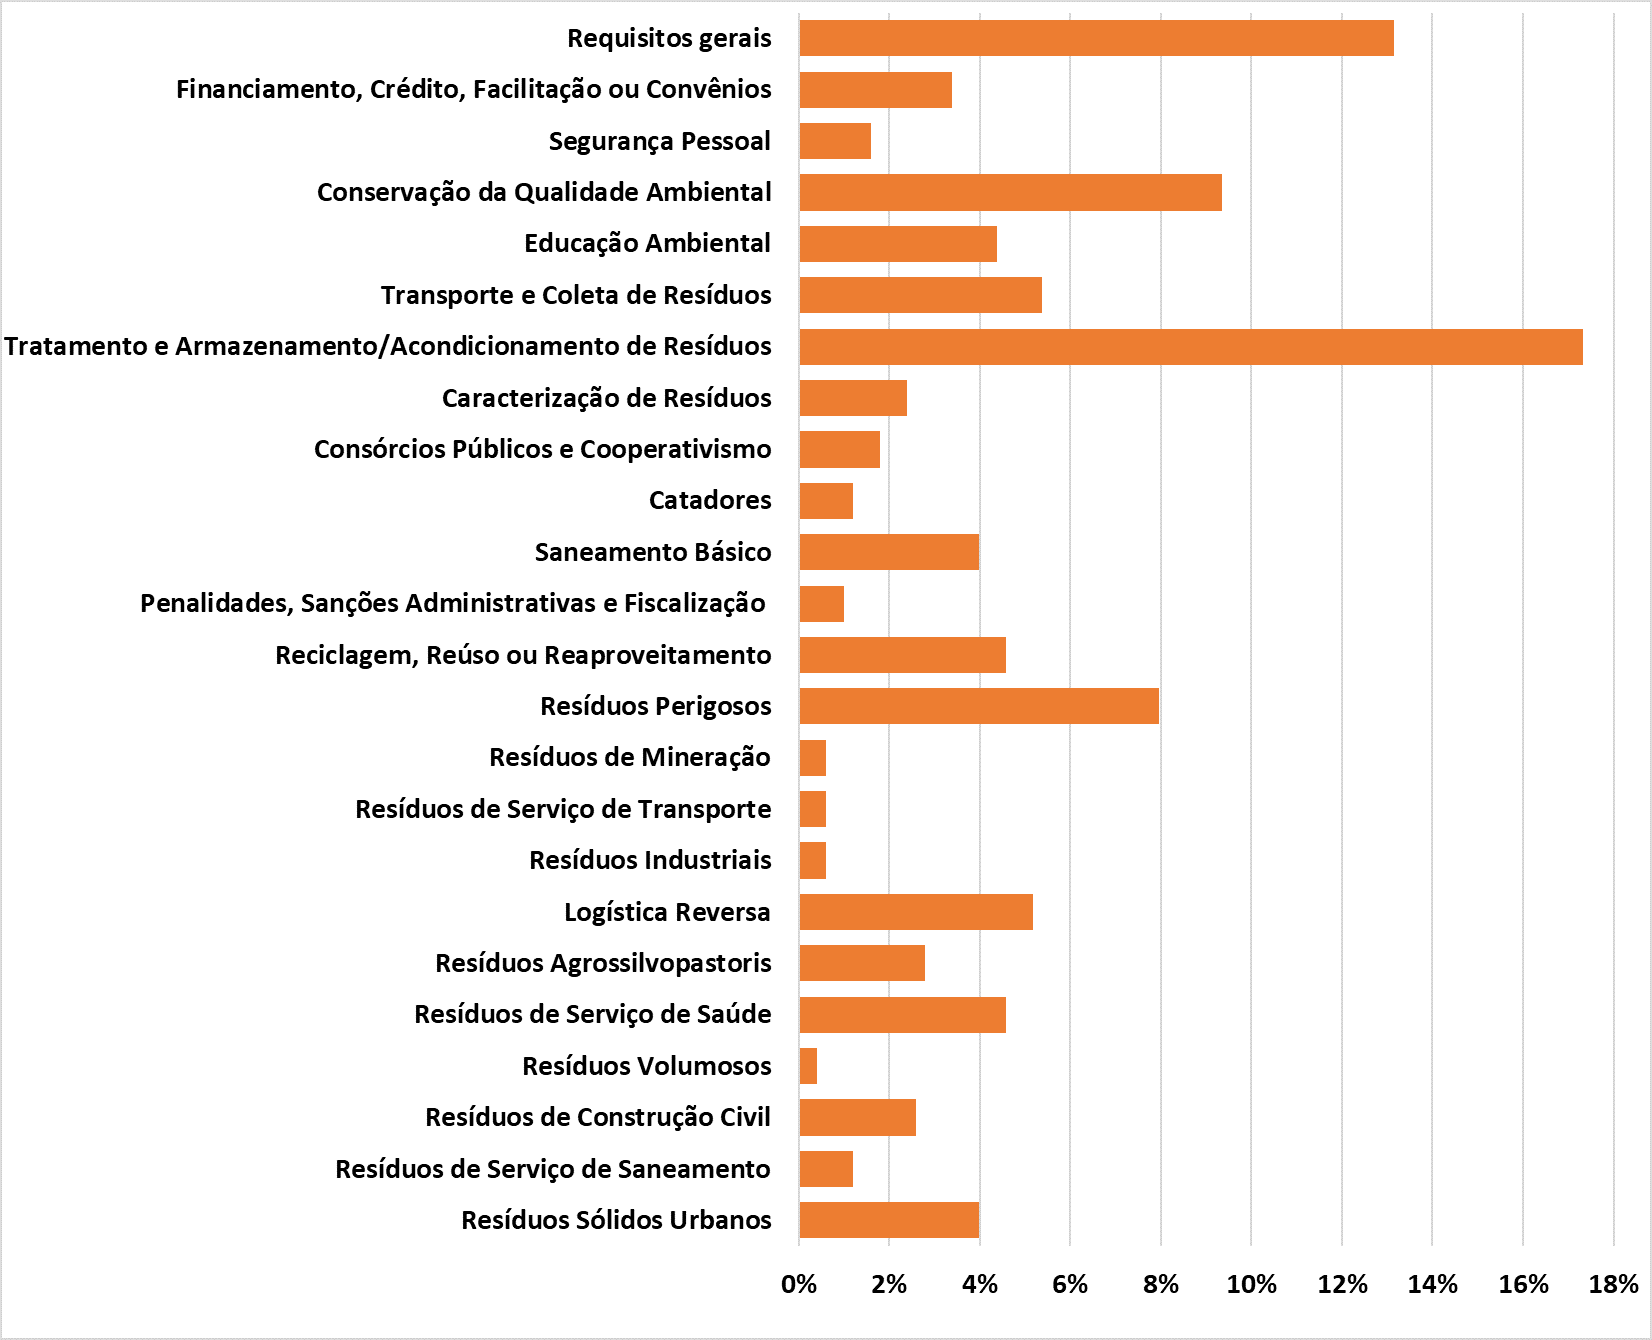
\includegraphics[width=\linewidth]{produtos/produm/distribuicaolegislacao}
		\caption{Distribuição de legislações e normas existentes por temas da gestão dos Resíduos Sólidos}
		\label{fig:distribuicaolegislacao}
	\end{figure}
	
	
	Observando a \autoref{fig:distribuicaolegislacao}, é possível verificar que a maioria das leis existentes é aplicada ao tema do tratamento e armazenamento/acondicionamento dos resíduos (17,3\% do total).
	
	Os resíduos perigosos, por sua vez, foram objeto principal de ações legisladoras, em maior parte, do governo federal. Não há, apesar do considerável número de leis de outras esferas da administração pública, nenhuma lei sobre esse tema na esfera pública municipal.
	
	Resíduos volumosos demandam grandes gastos de verbas públicas. Foi compilada apenas uma lei sobre a gestão de volumosos, municipal, que versa sobre a autorização de extrair e coletar podas de árvores volumosas ou não. Note-se que, apesar dos custos associados à gestão desse tipo de resíduos, não há nenhuma legislação específica sobre como realizar o gerenciamento de móveis, equipamentos domésticos, veículos inutilizados, entre outros.
	
	A fiscalização, juntamente com temas de sanções administrativas e penalidades, por sua vez, foi contemplada com cinco legislações em âmbito nacional e estadual e municipal, sendo apenas uma prescrita por Monteiro.
	
	Duas das legislações sobre fiscalização, uma federal e outra estadual, respectivamente, o Decreto federal Decreto 6.514/2008 e a resolução da secretaria de meio ambiente do estado de São Paulo 114/2010, versam sobre o gerenciamento de resíduos sólidos de um modo geral, com claras exigências em relação à conservação da qualidade ambiental. O único dispositivo legal municipal sobre a fiscalização, o Decreto municipal 753/1998, versa especificamente sobre a limpeza de ambientes públicos. Não há, na esfera da administração pública municipal, dispositivos legais específicos para a fiscalização de transporte, coleta, destinação final, gerenciamento de resíduos perigosos, educação ambiental, entre outros temas relevantes à gestão dos resíduos sólidos. 
	
	O tema referente à participação de catadores também foi contemplado com poucas legislações, sendo uma federal, duas estaduais e três, municipais, as quais equivalem a 1,2\% do total de leis e normas. Dentre as legislações municipais e estaduais, não há nenhuma que especifique a forma com que deve ocorrer a inclusão social e participação de catadores, o que poderia servir para detalhar assuntos abordados de forma geral pelo Programa Pró-Catador, do Decreto federal 7405/2010.
	
	A maior parte das leis e normas sobre gerenciamento de RSU foram elaboradas em nível estadual e municipal.  Diferentemente do que ocorre com os RSU, os resíduos de serviço de saneamento são quase totalmente regrados por meio de instrumentos legais e normativos em nível de federação. Os resíduos de serviços de saúde, agrossilvopastoris possuem instrumentos regulamentadores de todas as esferas de governo.
	
	Os resíduos da construção civil possuem maioria de legislações municipais. Ressalta-se a lei municipal 865/91, que versa sobre a doação de materiais de construção a famílias de baixa renda. Essa lei, caso seja implementada, poderá, ao mesmo tempo, diminuir os custos de disposição dos materiais descartados, ainda em condições de uso, e promover ganhos sociais.
	
	Os resíduos de logística reversa (pilhas e baterias, pneus, óleos lubrificantes e suas embalagens, lâmpadas fluorescentes e produtos eletroeletrônicos e seus componentes) não foram contemplados por nenhuma legislação municipal. A maior parte dos regramentos para a logística reversa foi feita pelo governo federal. Nesse contexto, percebe-se que não há detalhamentos em nível local sobre como o sistema logístico deverá ocorrer. Resíduos industriais não foram contemplados por nenhuma legislação municipal ou estadual, existindo somente em âmbito federal.
	
	De acordo com a administração municipal, serviços de transporte, tais como o transporte escolar, são indispensáveis à dinâmica econômica e cultural de Monteiro Lobato. No entanto, os resíduos gerados nesse setor, ainda não possuem regramentos específicos de gerenciamento, elaborados por ações legisladoras em nível regional ou local.
	
	Resíduos gerados por mineração não possuem leis estaduais. Além das exigências legais em nível federal, o município possui, em nível local, exigências sobre a prática de mineração e seus rejeitos gerados.
	
	
	%\newcolumntype{P}[1]{>{\centering\arraybackslash}p{#1}} %para centralizar valores das tabelas
\section{Introdução}

A Lei Federal nº 12.305 de 2010, que institui a Política Nacional de Resíduos Sólidos, visa a gestão integrada e o gerenciamento adequado dos resíduos sólidos, buscando a promoção da reciclagem e reutilização, além da destinação adequada dos resíduos sólidos, destacando também como um de seus princípios a responsabilidade compartilhada, atribuindo ao governo, fabricantes, comerciantes e consumidores a responsabilidade de minimizar o volume de resíduos sólidos e rejeitos gerados, bem como reduzir os impactos causados à saúde humana e à qualidade ambiental decorrentes do ciclo de vida dos produtos (BRASIL, 2010).

Apesar da responsabilidade, como um todo, não ser exclusiva de um ente específico, a limpeza urbana e a destinação final dos resíduos sólidos urbanos é de responsabilidade do poder público municipal, conforme art. 30 inciso V da Constituição Federal, que define os municípios como titulares dos serviços de interesse local, como é o caso da gestão de resíduos. A responsabilidade pelos resíduos gerados de atividades industriais, comerciais e serviços privados passam a ser do próprio gerador.

A Política Nacional de Resíduos Sólidos também introduz o PMGIRS como instrumento de planejamento, com horizonte temporal de 20 anos ou mais, cujo principal objetivo é de promover um diagnóstico da situação dos resíduos sólidos no município, estabelecer um prognóstico, com metas e indicadores adequados, além de prever soluções integradas, tornando-se um instrumento indispensável para o manejo de resíduos sólidos do município.


\section{Caracterização do município de Monteiro Lobato}

\subsection{Localização e acesso}

Localizado nas coordenadas médias 22º 57' 24" S; 45º 50' 23" O, com extensão territorial de 332,742 km² e distante 128 km da capital do estado de São Paulo, o município de Monteiro Lobato integra a Região Metropolitana do Vale do Paraíba (RMVP). Na \autoref{fig:image007} é possível observar os municípios pertencentes a RMVP.

\begin{figure}[hbt!]
	\centering
	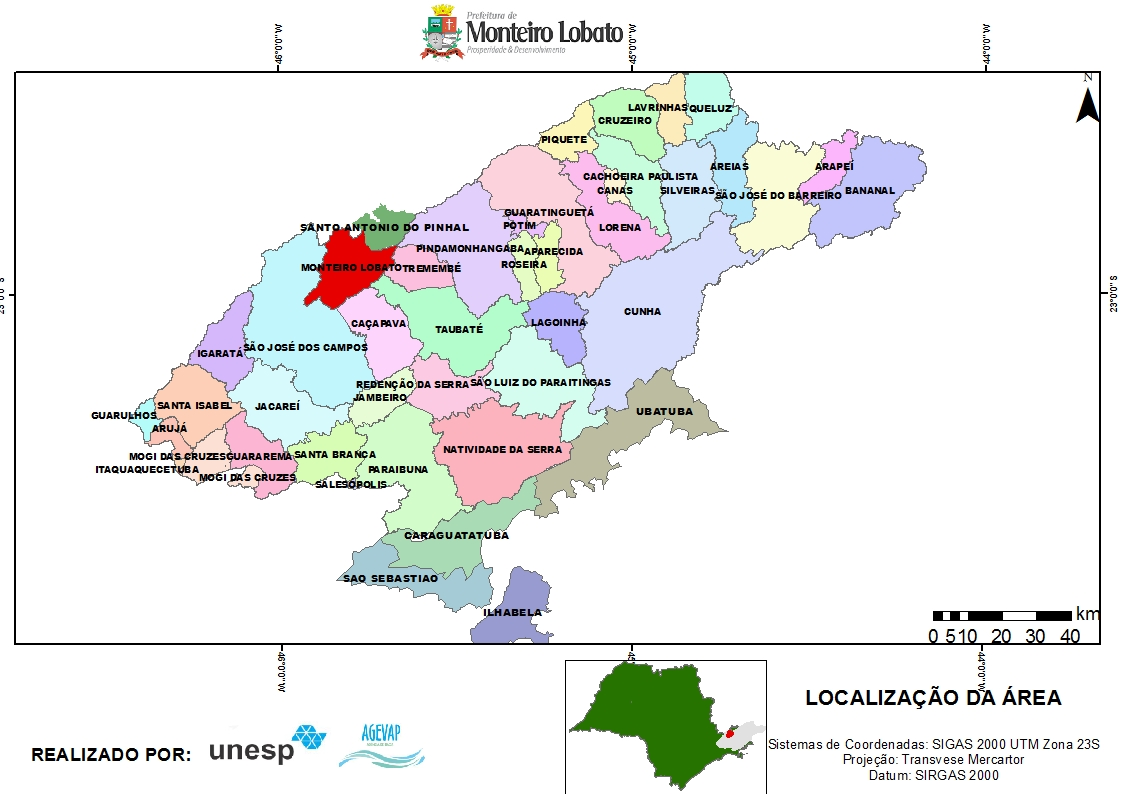
\includegraphics[width=1\linewidth]{produtos/proddois/image007}
	\caption{Divisão territorial dos municípios da RMVP}
	\legend{Fonte: IBGE, 2010 e EMPLASA, 2017}
	\label{fig:image007}
\end{figure}

O município faz divisa com os municípios de Sapucaí-Mirim (MG) e Santo Antônio do Pinhal (SP), ao norte; São José dos Campos e Caçapava, ao sul; com Taubaté e Tremembé, a leste; e com São Francisco Xavier, distrito de São José dos Campos, a oeste, como demonstrado na \autoref{fig:image008}. Tem como principais acessos, partindo de São Paulo, pelas rodovias BR-116 (Rodovia Presidente Dutra) ou pela SP-70 (Rodovia Carvalho Pinto) e posteriormente pela SP-50 (São José dos Campos/Campos do Jordão). Cabe destaque a essa última, frente à sua inserção na malha urbana de Monteiro Lobato ~\cite{MonteiroLobatoSite}.

\clearpage
\begin{figure}[hbt!]
	\centering
	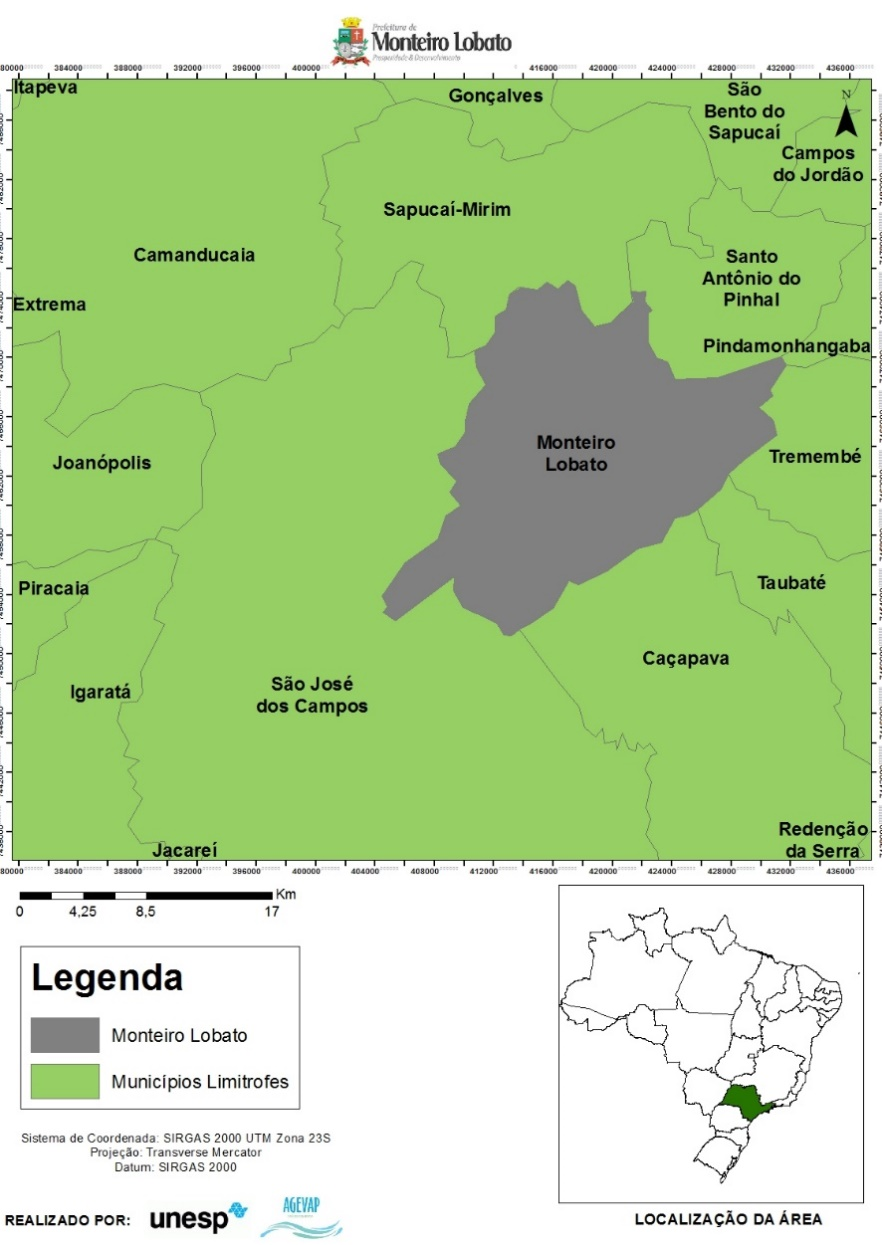
\includegraphics[width=0.9\linewidth]{produtos/proddois/image008}
	\caption{Mapa de localização de Monteiro Lobato no Brasil e no estado de São Paulo. }
	\legend{Fonte:~\cite{IBGE2010}}
	\label{fig:image008}
\end{figure}

\subsection{Bacia hidrográfica do rio Paraíba do Sul}
O município de Monteiro Lobato está inserido na bacia do rio Paraíba do Sul, que possui uma área de drenagem de 61.307 km² distribuída pelos estados de São Paulo (SP) (13.934 km²), Rio de Janeiro (RJ) (26.674 km²) e Minas Gerais (MG) (20.699 km²) (CEIVAP, AGEVAP, COHIDRO, 2014a). O Rio Paraíba do Sul é formado pela união dos rios Paraibuna e Paraitinga, na Serra da Bocaina, Estado de São Paulo, e sua foz encontra-se no município de São João da Barra, no Estado do Rio de Janeiro, a mais de mais de 1.100 km de suas nascentes. A bacia drena uma das regiões mais desenvolvidas do país, abrangendo parte do Estado de São Paulo, na região conhecida como Vale do Paraíba Paulista, parte do Estado de Minas Gerais, denominada Zona da Mata Mineira, e metade do Estado do Rio de Janeiro. A bacia abrange 184 municípios, 36 dos quais estão parcialmente inseridos na bacia. A população  total da bacia é 7,28 milhões de habitantes, dos quais 38\% (2,79 milhões) em SP, 39\% (2,86 milhões) no RJ e 22\% (1,63 milhão) em MG. O Sistema Hidráulico do Rio Paraíba do Sul, um complexo conjunto de reservatórios e estruturas hidráulicas existentes nas bacias hidrográficas do Paraíba do Sul e do Guandu, no Rio de Janeiro, é o responsável por reservar e transportar dois terços da vazão do Rio Paraíba do Sul para a bacia do Guandu, com o objetivo de gerar energia elétrica e garantir o abastecimento de cerca de nove milhões de pessoas na Região Metropolitana do Rio de Janeiro (KUMLER; LEMOS, 2008; ANA, 2015). Entre as décadas de 1930 a 1960 foram construídas as principais barragens ao longo do rio, quais sejam: Paraibuna/Paraitinga, Santa Branca, Funil, Santa Cecília e Ilha dos Pombos ~\cite{ANA2017}.

Deve-se destacar que o Sistema Hidráulico do Rio Paraíba do Sul é responsável por suprir de energia elétrica e água a cidade do Rio de Janeiro. Este sistema se subdivide em dois subsistemas:

\begin{itemize}
	\item Paraíba: compreende a transposição das águas do rio Paraíba do Sul em Santa Cecília. Esse subsistema é composto pela estação elevatória de Santa Cecília, barragem de Santana, estação elevatória de Vigário, usinas hidrelétricas Nilo Peçanha e Fontes Nova, reservatório de Ponte Coberta e usina hidrelétrica Pereira Passos;
	\item Lajes: consiste das barragens de Tocos e Lajes, calha da CEDAE e das Usinas Fontes Nova e Fontes Velha (está atualmente desativada).
\end{itemize}
\section{Histórico}

O nome do município Monteiro Lobato é uma referência ao escritor José Bento de Monteiro Lobato, reconhecido nacionalmente por sua influência na cultura do país. A região foi onde o escritor viveu e, em uma fazenda denominada “Fazenda do Visconde”, obteve inspiração para criar muitas de suas obras, incluindo muitos dos elementos que compuseram o ícone cultural de histórias infantis “Sítio do Pica-Pau Amarelo” ~\cite{squeff2003origem,IBGE2010}. As Figuras \ref{fig:image009} e \ref{fig:image010} mostram a fazenda em que o escritor viveu. 
 
\begin{figure}[h!]
	\centering
	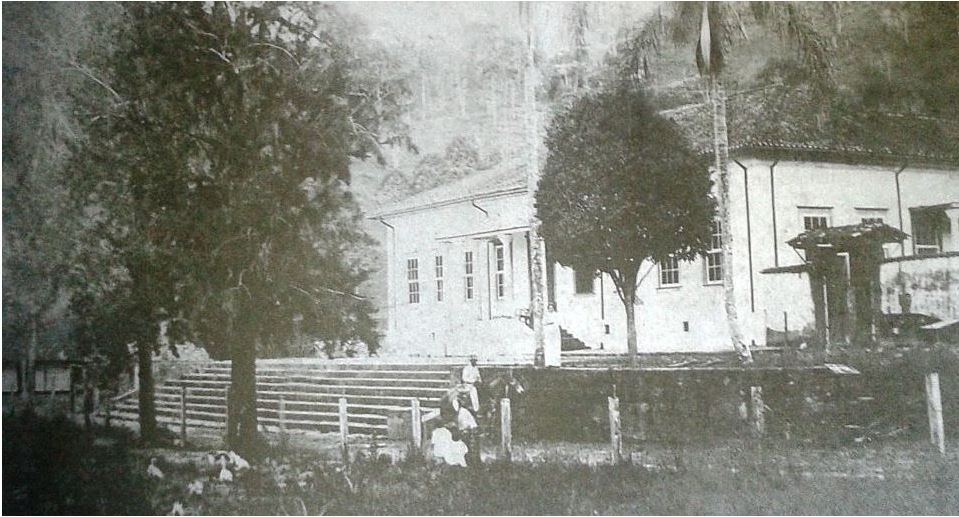
\includegraphics[width=0.8\linewidth]{produtos/proddois/image009}
	\caption{Fachada da frente da casa “Fazenda do Visconde”.}
	\legend{Fonte: Retirado do Site "O verdadeiro Sítio do Picapau Amarelo}
	\label{fig:image009}
\end{figure}

\begin{figure}[h!]
	\centering
	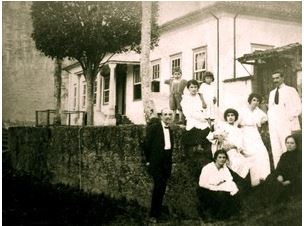
\includegraphics[width=0.55\linewidth]{produtos/proddois/image010}
	\caption{Monteiro Lobato ainda criança em frente ao casarão da fazenda em que morava.}
	\legend{Fonte: Arquivo Pessoal/André Barreto.}
	\label{fig:image010}
\end{figure}

Segundo a Prefeitura de Monteiro Lobato, antes deste nome, a localidade que era incluída dentro dos limites do município de Taubaté, e possuiu quatro nomes: Freguesia das Estacas, Freguesia de Nossa Senhora do Bonsucesso do Buquira, Vila das Palmeiras do Buquira e Vila do Buquira ~\cite{MonteiroLobatoSite}. Entretanto, era comumente denominada apenas como Buquira, que em tupi-guarani significa “Ribeirão dos Pássaros”, por situar-se à uma das margens do rio Buquira ~\cite{IBGE2010}.

Em 1857, Buquira foi denominada como Freguesia e Distrito de Paz até que em 1900 ascendeu à condição de Vila. Em 1934 ascendeu a cidade, por lei estadual, entretanto no mesmo ano, ainda com a nomenclatura de Buquira, foi reduzida à condição de distrito e incluída ao município de São José dos Campos, até ser emancipada em 1948 para então, um ano depois, receber o atual nome ~\cite{MonteiroLobatoSite}.

A história do município está inserida no contexto do Vale do Paraíba como caminho dos bandeirantes e dos tropeiros, participando também dos ciclos econômicos do café e da pecuária leiteira. Houve, no município, períodos de prosperidade que foram seguidos de períodos de estagnação econômica, provocando assim, o êxodo de parte de sua população ~\cite{MonteiroLobato2014}.

O movimento da Rodovia Monteiro Lobato (SP-50), que liga São José dos Campos a Campos do Jordão, contribuía para o pequeno comércio local com as paradas dos viajantes que, mesmo em curto período de tempo, consumiam produtos característicos da cidade. Entretanto, com a construção da Rodovia Floriano Rodrigues Pinheiro (SP-123) em 1978, ligando Taubaté a Campos do Jordão, Monteiro Lobato teve sua economia novamente prejudicada ~\cite{MonteiroLobato2014}.

Por outro lado, embora estrategicamente localizado no caminho para São Francisco Xavier, distrito de São José dos Campos, e para Campos do Jordão e sul de Minas Gerais, seu desenvolvimento econômico lento colaborou para o que hoje são os seus maiores atrativos turísticos: a preservação de 50,80\% da vegetação do município e suas características de uma pequena cidade rural com vida tranquila ~\cite{MonteiroLobato2014}.

\section{Turismo, cultura e lazer}

De acordo com o artigo 2º da Lei N° 11.771, de 17 de setembro de 2008, que dispõe sobre a Política Nacional de Turismo e dá outras providências, é considerado turismo as atividades realizadas por pessoas físicas durante viagens e estadias em lugares diferentes do seu entorno habitual, por um período inferior a 1 (um) ano, com finalidade de lazer, negócios ou outras.
No Brasil, a participação direta do turismo na economia foi de US\$ 56,8 bilhões em 2016, o equivalente a 3,2\% do PIB. Já a contribuição total do setor foi de US\$ 152,2 bilhões, 8,5\% do PIB Nacional. Segundo dados da World Travel \& Tourism Council (WTTC), o setor de turismo gerou mais de 7 milhões de empregos em 2016, o que representa 7,8\% do total de empregos. Estão incluídas, como geradoras de empregos diretos, as atividades relacionadas a hotelaria, agências de turismo, companhias aéreas, demais tipos de transportes de passageiros e turistas, além de restaurantes e empreendimentos de lazer ~\cite{PNT2018}.

O município de Monteiro Lobato conta com um Plano Diretor de Turismo Sustentável de Monteiro Lobato (P), elaborado pelo Grupo de Planejamento Participativo do Turismo Sustentável de Monteiro Lobato (PlaneJÁtur). Como um documento complementar, há um Plano de Desenvolvimento Turístico Municipal de Monteiro Lobato (PDTM) elaborado por uma parceria entre o curso de Turismo na Universidade de São Paulo (USP) e a Prefeitura Municipal de Monteiro Lobato, iniciado em 2013.

A cidade possui diversos monumentos, construções e manifestações culturais que podem ser considerados patrimônio histórico cultural da cidade. Os mesmos são registros da cultura, tradições e/ou história local e se mostram de extrema importância para manter a identidade do município (PDTM, 2013).

A Igreja Matriz, por exemplo, simboliza a origem do município, pois foi a partir dela que houve o surgimento da Freguesia, que, futuramente, viria a se transformar no Município de Monteiro Lobato. A arquitetura da cidade, principalmente na região central, manteve-se, em sua maior parte, preservada, o que contribuiu para a manutenção da identidade do município e também se alia aos seus aspectos imateriais, caracterizados por seus saberes locais, suas festas tradicionais e populares, além do ambiente de tranquilidade e com características caipiras ainda preservados na cidade (PDTM, 2013).

A maior influência cultural e artística do município se dá pelos contos do Sítio do Pica-Pau Amarelo, escritos por José Bento Monteiro Lobato, no período em que viveu no local e deu início à essa obra literária de grande relevância na Literatura Infantil Brasileira. O casarão onde o escritor morou é aberto ao público e administrado por Maria Lucia Ribeiro, o sítio lobatense conta com dezoito cômodos compostos por bibliotecas e mobília do início século passado. Além do casarão como construção principal, a propriedade possui uma extensa área verde e uma cachoeira conhecida como “Reino das Águas Claras”, batizada pelo próprio Lobato.

Os contos do Sítio do Pica-Pau Amarelo acarretam, atualmente, na propagação de diversas lendas no cotidiano do lobatense, desde personagens folclóricos como o Saci e criaturas da mitologia. Além disso, disseminam o artesanato local como bonecas da personagem Emília e outros presentes na obra; tanto quanto o comércio e a infraestrutura local como nomes de restaurantes e escolas.

Desde o ano de 2010, acontece no município o Festival de Literatura Infantil, sempre no mês de setembro com todas as atividades gratuitas. Com o objetivo de preservar a memória do escritor José Bento Monteiro Lobato, incentivar a leitura e formar novos leitores. As figuras \ref{fig:image011}, \ref{fig:image012} e \ref{fig:image013} mostram alguns registros fotográficos do Festival.

 \begin{figure}[h!]
 	\centering
 	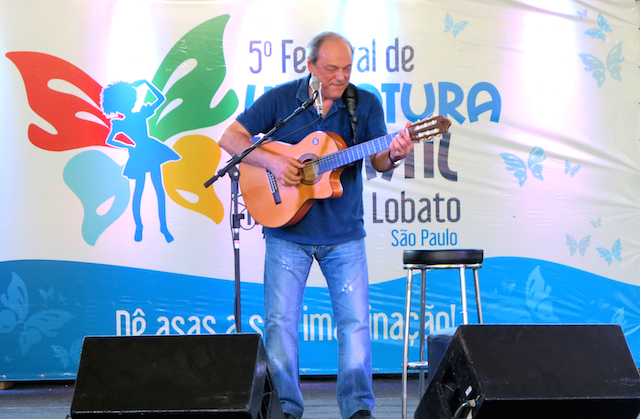
\includegraphics[width=0.75\linewidth]{produtos/proddois/image011}
 	\caption{Festival de Literatura Infantil em Monteiro Lobato de 2014 – Parte I.}
 	\legend{Fonte: Prefeitura de Monteiro Lobato.}
 	\label{fig:image011}
 \end{figure}

 \begin{figure}[h!]
 	\centering
 	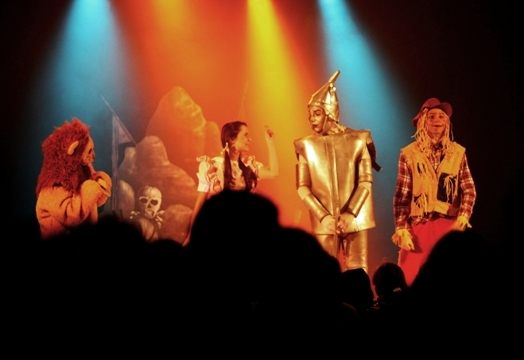
\includegraphics[width=0.75\linewidth]{produtos/proddois/image012}
 	\caption{Festival de Literatura Infantil em Monteiro Lobato de 2014 – Parte II.}
 	\legend{Fonte: Prefeitura de Monteiro Lobato.}
 	\label{fig:image012}
 \end{figure}

 \begin{figure}[h!]
	\centering
	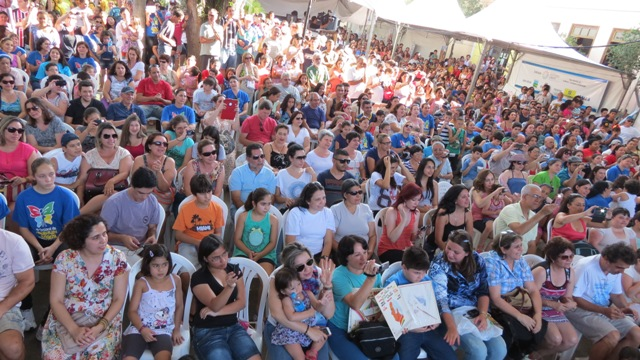
\includegraphics[width=0.75\linewidth]{produtos/proddois/image013}
	\caption{Festival de Literatura Infantil em Monteiro Lobato de 2014 – Parte III.}
	\legend{Fonte: Prefeitura de Monteiro Lobato.}
	\label{fig:image013}
\end{figure}

Outros festivais, manifestações e tradições culturais de alto impacto no munícipio são os Pereirões, os Grupos Moçambique Esperança e Catira União Lobatentes (grupos dançantes). Os Pereirões são bonecos gigantes associados à época de Carnaval, possuem corpos de jacá, um cesto feito de bambu e cipó e altura superior a três metros, como mostra a \autoref{fig:image014}. A estrutura é carregada pelos foliões durante a celebração, que realizam danças, giros e corridas com o público.


 \begin{figure}[!h]
	\centering
	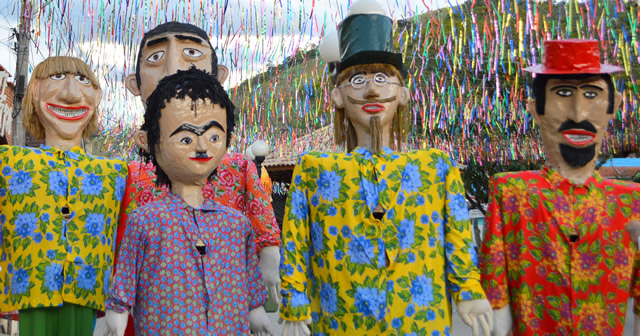
\includegraphics[width=0.75\linewidth]{produtos/proddois/image014}
	\caption{Pereirões de Monteiro Lobato.}
	\legend{Fonte: Prefeitura de Monteiro Lobato.}
	\label{fig:image014}
\end{figure}

O Grupo Catira surgiu da década de 1930 pelos irmãos Francisco Rosa e Antônio Rosa, e é marcado por passos firmes e palmas sincronizadas, ritmo composto pelo som da viola caipira, entoado por dois violeiros. A dança é executada em duas fileiras – uma em frente à outra, formando pares. O chapéu é uma peça fundamental. O Grupo Moçambique Esperança é um grupo que repercute uma dança de origem africana e que chegou ao município no ano de 1940. Com movimentos ritmados, produz belos efeitos sonoros. Utilizam bastões que servem para marcar o ritmo da dança, além de instrumentos de percussão e corda. Os grupos supracitados são mostrados na \autoref{fig:image015} e \autoref{fig:image016} respectivamente.


 \begin{figure}[h!]
	\centering
	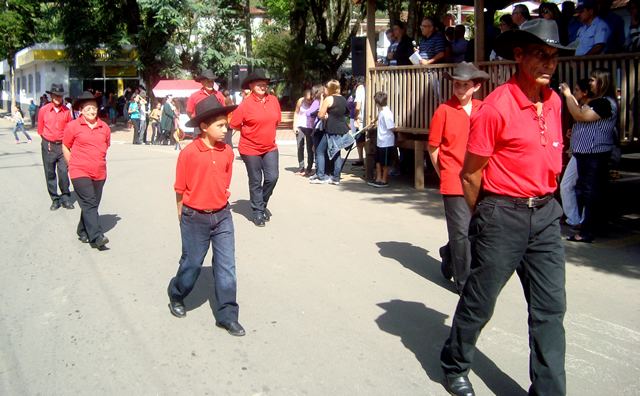
\includegraphics[width=0.85\linewidth]{produtos/proddois/image015}
	\caption{Grupo Catira de Monteiro Lobato.}
	\legend{Fonte: Prefeitura de Monteiro Lobato.}
	\label{fig:image015}
\end{figure}

 \begin{figure}[h!]
	\centering
	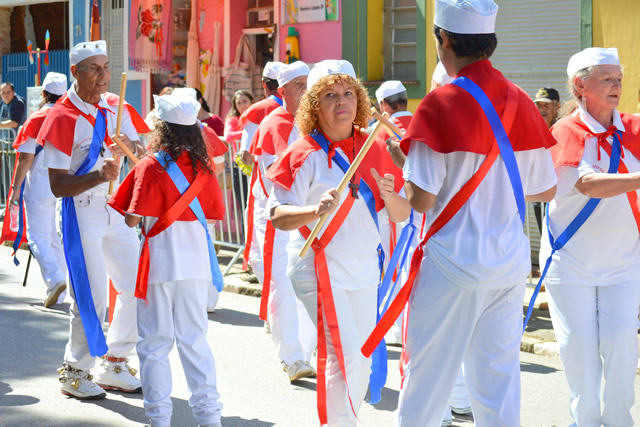
\includegraphics[width=0.85\linewidth]{produtos/proddois/image016}
	\caption{Grupo Moçambique Esperança.}
	\legend{Fonte: Prefeitura de Monteiro Lobato.}
	\label{fig:image016}
\end{figure}

Ademais, o município tem fortes influências da Igreja Católica e possui diversas festas religiosas que acontecem no decorrer do ano. No mês de janeiro acontecem homenagens a São Sebastião; no mês de maio, Santa Rita de Cássia é venerada no bairro do Souza; e em setembro ocorre a comemoração em torno da padroeira, Nossa Senhora de Bonsucesso.
\clearpage

\section{Geografia física}

A geografia física corresponde ao meio de suporte sobre o qual se desenvolve tanto o meio biótico, objeto do próximo item, como o meio antrópico. Os temas a serem abordados correspondem ao solo, água e ar, mas são aqui tratados dentro de uma perspectiva que objetiva descrever as características locacionais do município para potenciais infraestruturas de gestão de Resíduos Sólidos. Os dados aqui apresentados foram coletados e produzidos pelo Instituto de Pesquisas Tecnológicas - IPT no ano de 2016, como parte do diagnóstico de base para o novo Plano Diretor para a cidade de Monteiro Lobato.

\subsection{Clima}

A classificação climática de Köppen é uma classificação baseada no pressuposto de que a vegetação natural é a melhor expressão do clima de uma região e as modificações críticas ao sistema são sempre relacionadas aos limites térmicos/hídricos dos tipos de climas determinados para diferentes regiões. Assim, as fronteiras entre regiões climáticas foram selecionadas para corresponder, tanto quanto possível, às áreas de predominância de cada tipo de vegetação, razão pela qual a distribuição global dos tipos climáticos e a distribuição dos biomas apresenta elevada correlação ~\cite{Rolim2007}. Segundo essa classificação, Monteiro Lobato possui clima do tipo Cwa, considerado um clima temperado úmido com Inverno seco e Verão quente. Com temperatura média anual de 20,9°C, oscilando entre mínima média de 14,6°C e máxima média de 27,2°C.

A precipitação média total anual é de 1870,4 mm. A \autoref{fig:image017} mostra o panorama da precipitação média mensal, entre 1939 e 2004, onde é possível observar a distribuição da precipitação ao longo do ano, com destaque para o período de inverno seco, descrito anteriormente ~\cite{MonteiroLobato2014}.
\clearpage
 \begin{figure}[h!]
	\centering
	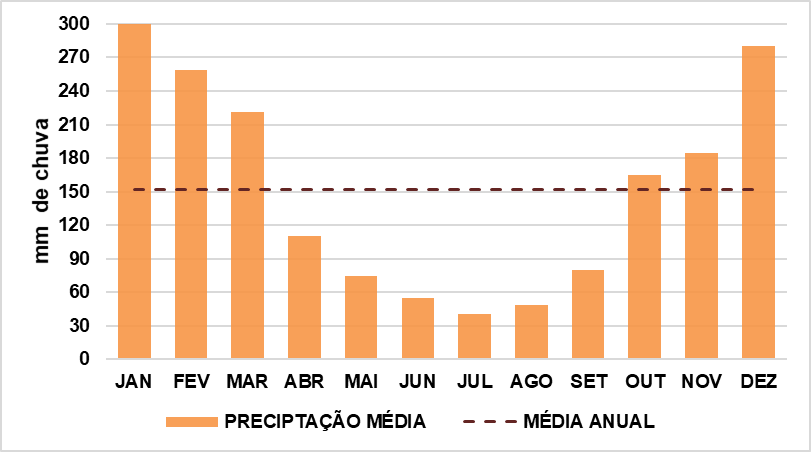
\includegraphics[width=1\linewidth]{produtos/proddois/image017}
	\caption{Precipitações médias mensais no período de 1939 a 2004.}
	\legend{Fonte: ~\cite{MonteiroLobato2014}}.
	\label{fig:image017}
\end{figure}


\subsection{Geologia}

O município de Monteiro Lobato é formado pelas seguintes unidades geológicas: Complexo Embu, Complexo Varginha-Guaxupé, depósitos aluvionares, Formação Boturana e maciços graníticos, além de falhas geológicas. O Complexo Embu é formado por xistos, filitos, migmatitos, gnaisses migmatizados e corpos lenticulares de quartzitos, anfibolitos e rochas calciossilicatadas e possui afloramentos com direção NE-SW. Já o Complexo de Varginha-Guaxupé é formado por gnaisses neoproterozóicos, de origem ígnea e sedimentar. Este complexo é dividido em três unidades: Granulítica Basal, Ortognáissica Migmatítica Intermediária e Paragnáissica Migmatítica Superior.  Ao menos as duas unidades superiores são intrudidas por um granitóide cedo a sin-colisional que ocorre restrito ao domínio do Complexo Varginha-Guaxupé. A Formação Boturuna é formada pormetapelitos com lentes de quartzitos na base e rochas carbonáticas no topo. Os depósitos aluvionares, por sua vez, são formados por depósitos sedimentares gerados pelo transporte de material realizado pelas águas correntes ~\cite{CPRM}.

A \autoref{fig:image018} mostra as unidades geológicas distribuídas pelo território do município de Monteiro Lobato. Através dela, pode-se perceber que as unidades geológicas predominantes são o Complexo de Embu e o Complexo de Varginha-Guaxupé.

\begin{figure}[h!]
	\centering
	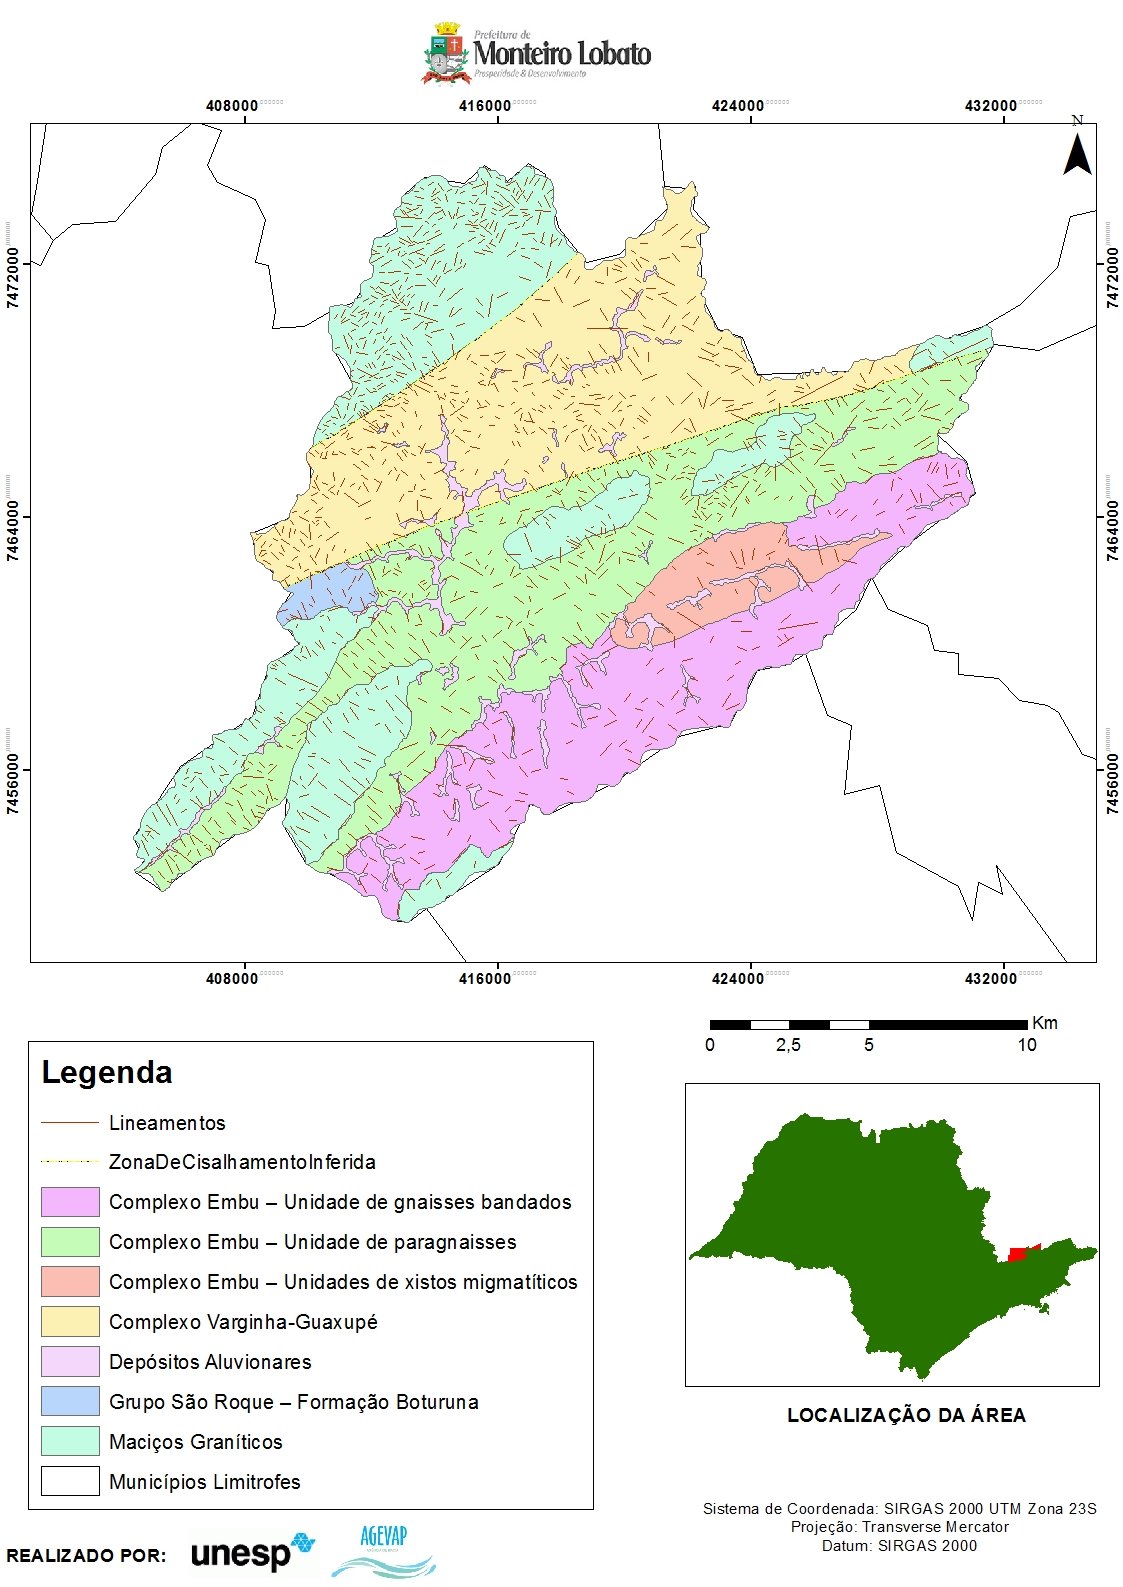
\includegraphics[width=0.85\linewidth]{produtos/proddois/image018}
	\caption{Unidades geológicas do Município de Monteiro Lobato.}
	\legend{Fonte: Adaptado IPT, 2016.}
	\label{fig:image018}
\end{figure}
\clearpage

\subsection{Geomorfologia}

Segundo Ab’Sáber (2007), Monteiro Lobato está situada no domínio morfoclimático tropical-atlântico, chamado de “mares de morros” florestados. Esse domínio apresenta a seguinte combinação de fatos fisiográficos: decomposição funda e universal das rochas cristalinas ou cristalofilianas, de 3 a 5 até 40 a 60 m de profundidade; presença de solo de tipo latossolo ou pedosolo amarelo-vermelho; superposição de solos devido às flutuações climáticas finais do quaternário em sertões sincopados; mamelonização universal das vertentes, desde o nível de morros altos até os níveis dos morros intermediários e patamares de relevo; drenagem originalmente perene até para o menor dos ramos das redes hidrográficas dendríticas regionais; lençol d’água subterrâneo que alimenta permanentemente, durante e entre as chuvas, a correnteza dos leitos dos cursos d’água; forte cota de umidade do ar; equilíbrio sutil entre processos morfoclimáticos, pedológicos, hidrológicos e ecossistêmicos.

A paisagem natural é o resultado de diferentes elementos que compõem o meio físico como rocha, relevo, solo e vegetação. Neste contexto, a compreensão e a identificação das diferentes formas de relevo se constituem componente de grande importância na implantação de qualquer atividade antrópica que altere significativamente a paisagem. O município de Monteiro Lobato se localiza em um território com colinas, escarpas, morros altos, morros baixos, morrotes, serras, planícies e terraços fluviais. Entretanto, de acordo com o Plano Diretor do Turismo Sustentável de Monteiro Lobato (2014), 59,72\% da área do município está entre as cotas altimétricas de 700 a 1.000 m, que representam a transição entre o relevo de morros e as escarpas da Serra da Mantiqueira. As maiores altitudes aparecem ao norte do município na divisa com o município de Santo Antônio do Pinhal e na divisa com o Estado de Minas Gerais. As menores altitudes estão associadas ao sul do município e às várzeas dos rios Ferrão ou Buquira e Buquirinha \autoref{fig:image019}. 

Essa configuração de relevo pode propiciar o aparecimento de fenômenos naturas de movimentos de massa, o que inclui escorregamentos, quedas de blocos e rastejos (movimentos lentos nos solos). Nestas áreas de concentração, os principais fragmentos de floresta têm um importante papel na perenização das nascentes, na infiltração da água no solo e na regulação do escoamento de base. Com a remoção destas florestas, as áreas de serras e escarpas passam a funcionar, hidrologicamente, como áreas com grande volume e elevada velocidade do escoamento superficial \textbf{(SIMÕES, 2012).}

 \begin{figure}[h!]
 	\centering
 	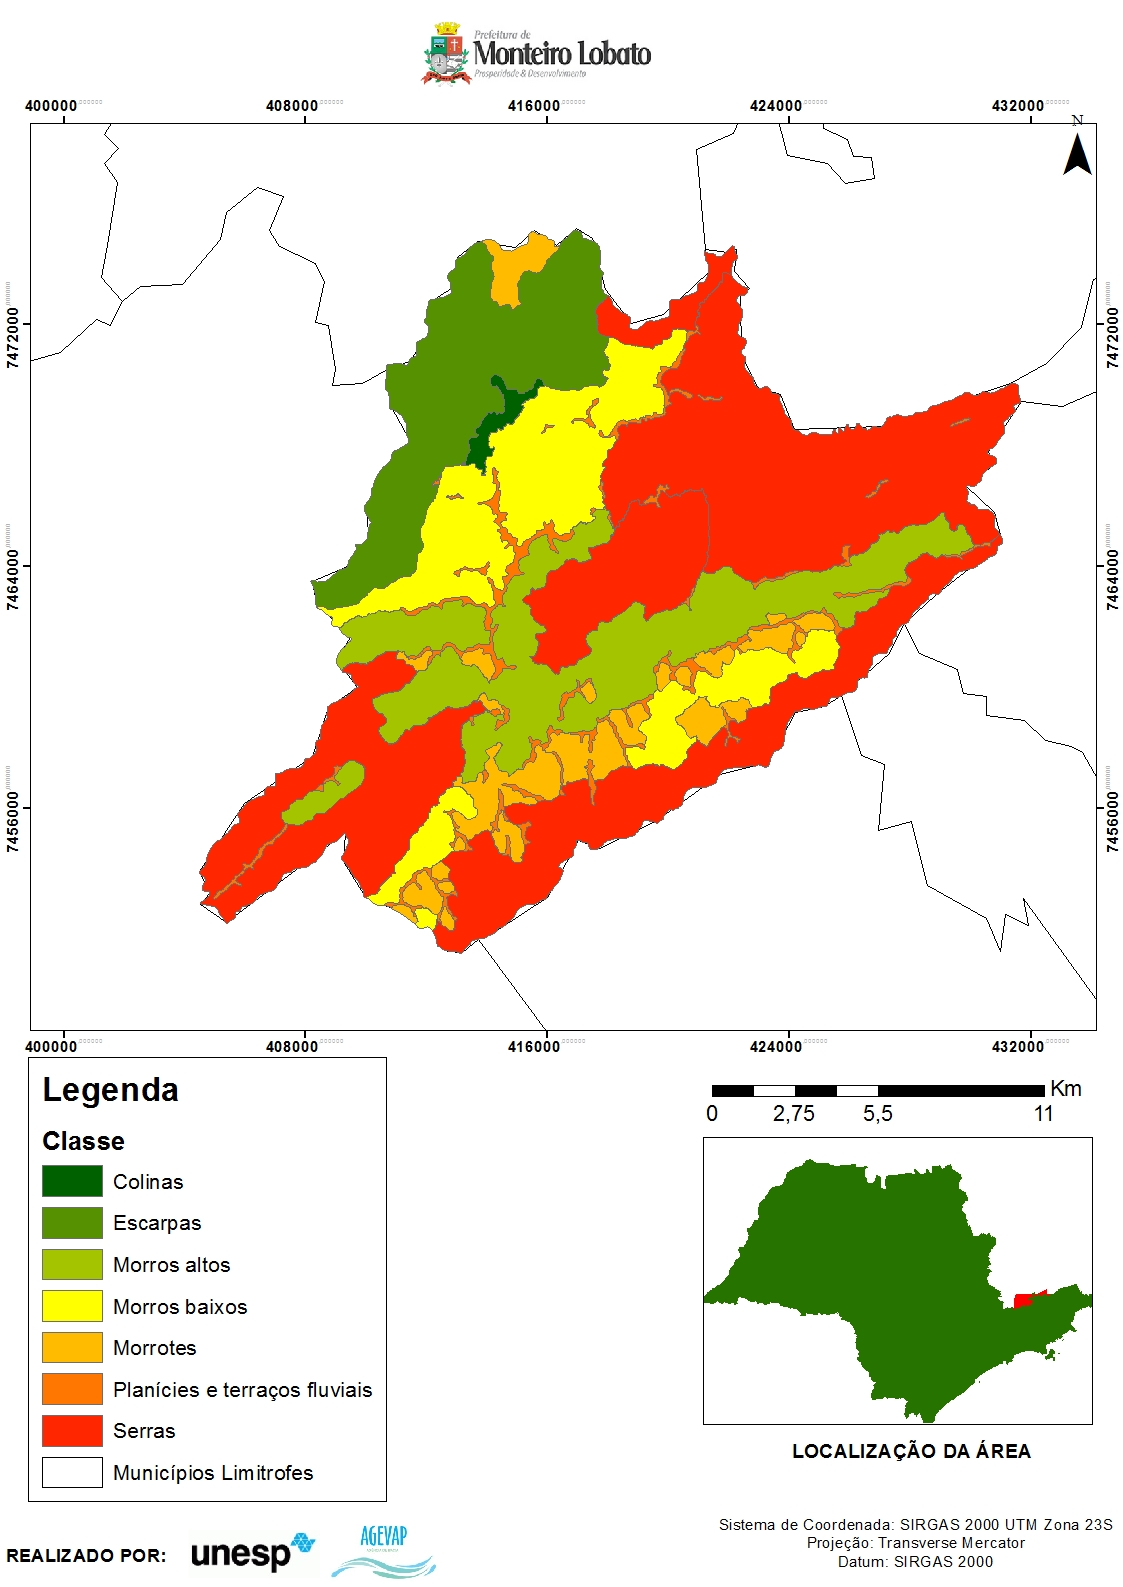
\includegraphics[width=0.85\linewidth]{produtos/proddois/image019}
 	\caption{Unidades geomorfológicas no munício de Monteiro Lobato -SP.}
 	\legend{Fonte: Adaptado IPT, 2016.}
 	\label{fig:image019}
 \end{figure}
\clearpage
\subsection{Relevo}

Monteiro Lobato está localizada nas escarpas e reversos da Serra da Mantiqueira, apresentando uma topografia montanhosa. A área urbana está a 650 m de altitude em relação ao nível do mar. Por esses fatores, a declividade no munícipio é um elemento decisivo que interfere de forma significativa na distribuição de classes de solos, bem como exerce influência nos processos de erosão, exigindo manejos agrícolas diferenciados para uma ocupação adequada das terras ~\cite{MonteiroLobato2014}.

A \autoref{fig:image020} nos permite aferir que as declividades menores estão   associadas às áreas de várzeas dos rios Buquira/Ferrão e Buquirinha. Ela mostra também como a declividade média de Monteiro Lobato varia entre 17-20º, sendo que em sua maioria, o munícipio apresenta áreas bastante declinosas (>20º).
\newpage
\begin{figure}[h!]
	\centering
	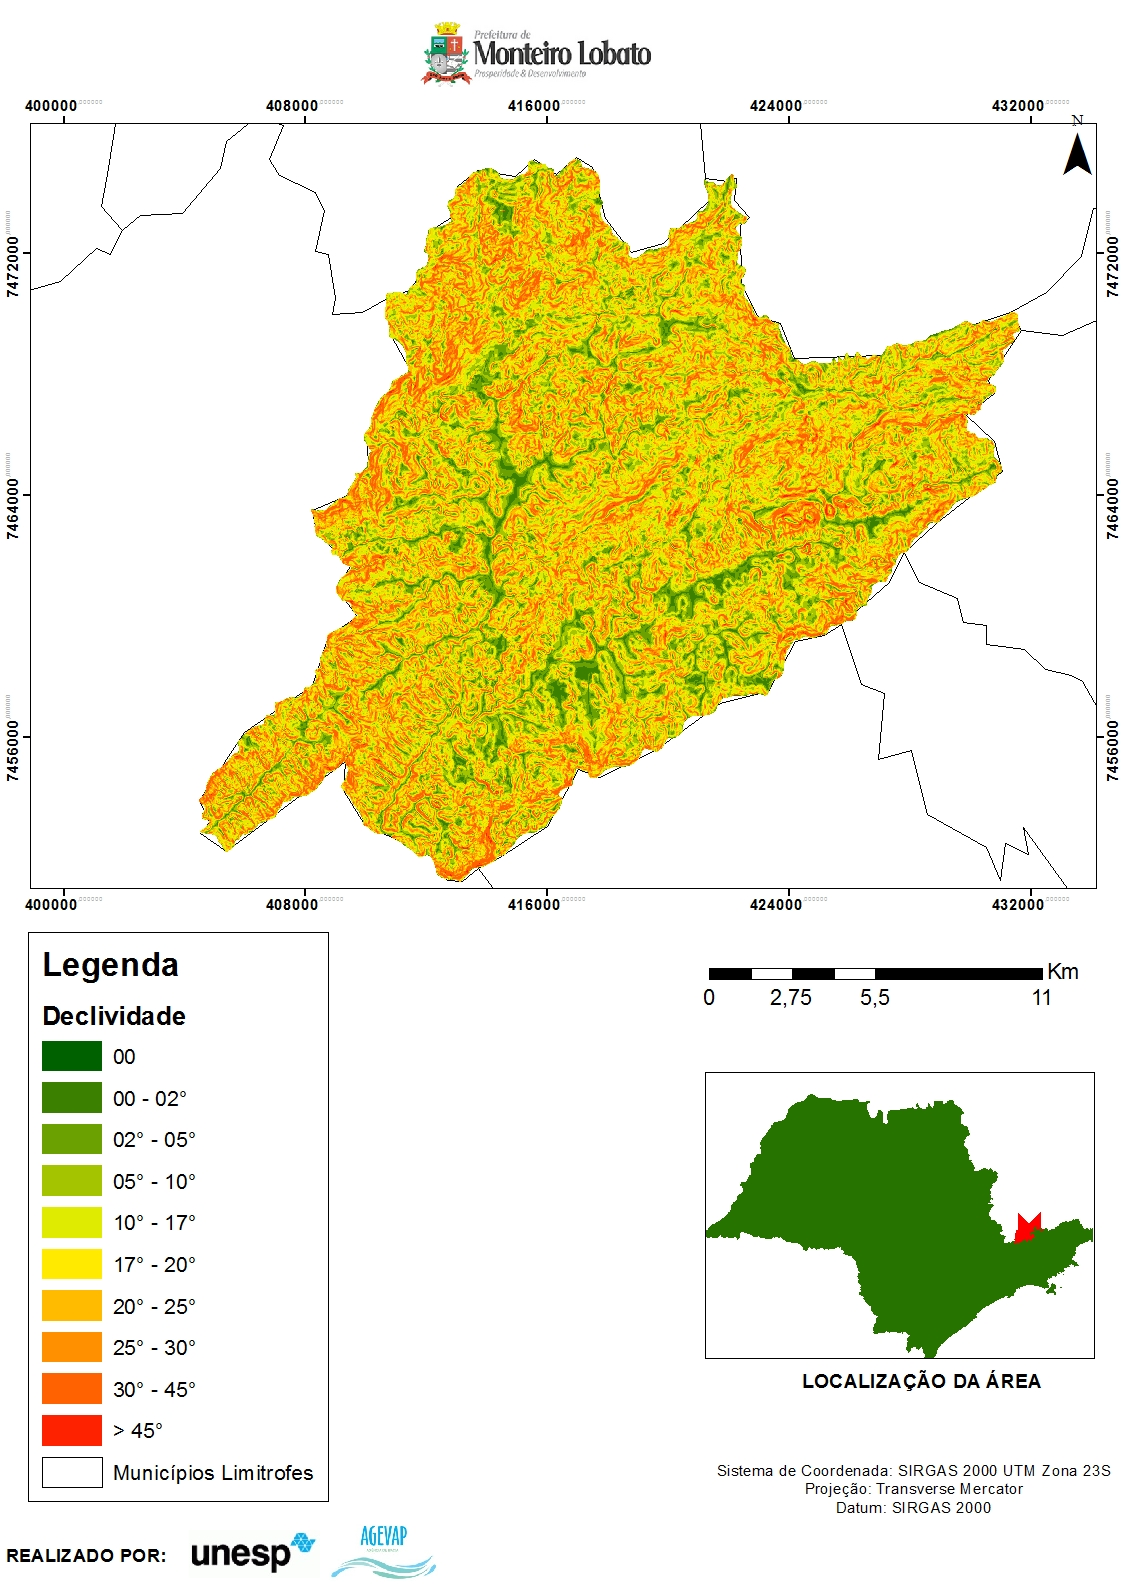
\includegraphics[width=1\linewidth]{produtos/proddois/image020}
	\caption{Declividade do município de Monteiro Lobato -SP.}
	\legend{Fonte: Adaptado IPT, 2016.}
	\label{fig:image020}
\end{figure}
\clearpage
\subsection{Recursos naturais}

Em Monteiro Lobato, o tipo de vegetação predominante é a Floresta Ombrófila Densa, cuja característica mais marcante é a presença de árvores altas, atingindo entre 20 e 30 m.  Estas árvores possuem folhas largas e sempre verdes de longa duração (perenifólias), além de mecanismos adaptados para resistir tanto a períodos de calor extremo, quanto de muita umidade. Entretanto, a cobertura vegetal natural não se encontra mais em seu estado original, pois delas já foram removidas as árvores de grande porte fornecedoras de madeira. Mesmo assim, Monteiro Lobato preserva 50,80\% de sua vegetação nativa, somando 16.912 hectares ~\cite{MonteiroLobato2014}.

O município possui em seu território parte de uma unidade de conservação de uso sustentável, a Área de Preservação Ambiental (APA) da Bacia do Rio Paraíba do Sul, além da Reserva Particular de Patrimônio Natural (RPPN) Sítio do Cantoneiro \autoref{fig:image021}, que contribuem para a manutenção da vegetação natural restante no município. 

No estudo produzido por Arcorverde 2018, que ranqueia os municípios da região metropolitana do Vale do Paraíba e Litoral Norte do estado de São Paulo, com uma faixa entre 0 e 1 para os desempenhos Ambientais, socioeconômico e institucional, posicionou Monteiro Lobato como o 10° município entre os 39 avaliados.   Dentre os índices de desempenho, Monteiro Lobato foi ranqueado com 0,60 para ambiental, 0,33 para socioeconômico e 0,1 para institucional ~\cite{arcoverdeproposiccao} aproximadamente. 
\newpage
\begin{figure}[h!]
	\centering
	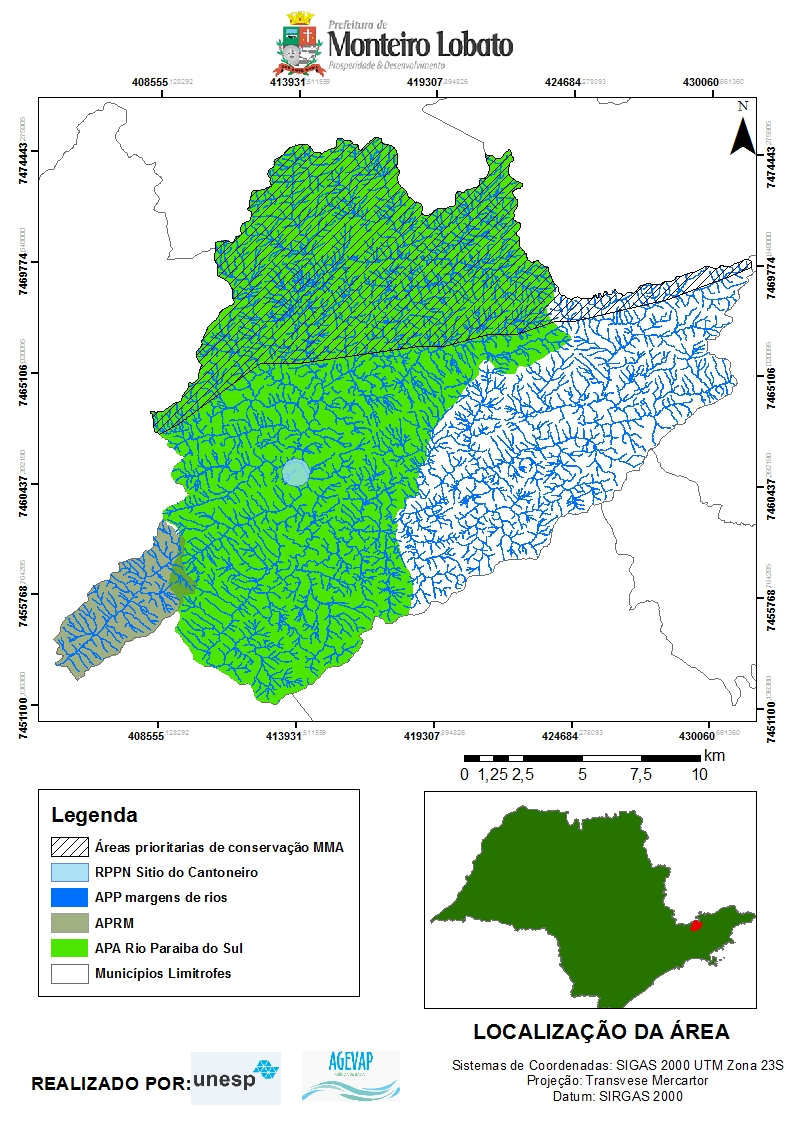
\includegraphics[width=1\linewidth]{produtos/proddois/image021}
	\caption{Recurso naturais do município de Monteiro Lobato -SP.}
	\legend{Fonte: Adaptado IPT, 2016.}
	\label{fig:image021}
\end{figure}
\clearpage
\subsection{Hidrografia}

A UGRHI  02 – Paraíba do Sul é constituída pela Bacia do Rio Jaguari e de outros tributários do Rio Paraíba do Sul, tanto da margem esquerda como da direita, desde as nascentes de seus formadores (rios Paraibuna e Paraitinga) até a divisa dos Estados de São Paulo e do Rio de Janeiro, a montante da barragem do Funil. Em condições naturais, a UGRHI - 02 não recebe contribuições nem deságua em outras bacias hidrográficas do Estado de São Paulo. Os principais afluentes do Rio Paraíba do Sul no seu trecho paulista são: o Paraibuna, o Paraitinga, o Jaguari, o Una, o Buquira/Ferrão, o Embaú/Piquete, o Bocaina e o Pitangueiras/Itagaçaba ~\cite{MonteiroLobato2014}.

A sub-bacia do Rio Buquira, no município de Monteiro Lobato, integrada à bacia do Rio Paraíba do Sul, é composta, entre outros, pelos rios Buquira/Ferrão, Braço e Descoberto; pelo córrego do Machado e pelos ribeirões Souzas e Matinada. Monteiro Lobato apresenta uma rede de drenagem densa, o que faz dos recursos hídricos um fator importante para a cidade \autoref{fig:image022}. Na figura citada entende-se por curso d’água os elementos como: rios, ribeirões, córregos, riachos etc. e, por corpo d’água:  lagos, lagoas, zonas úmidas etc. 

\newpage
 \begin{figure}[h!]
 	\centering
 	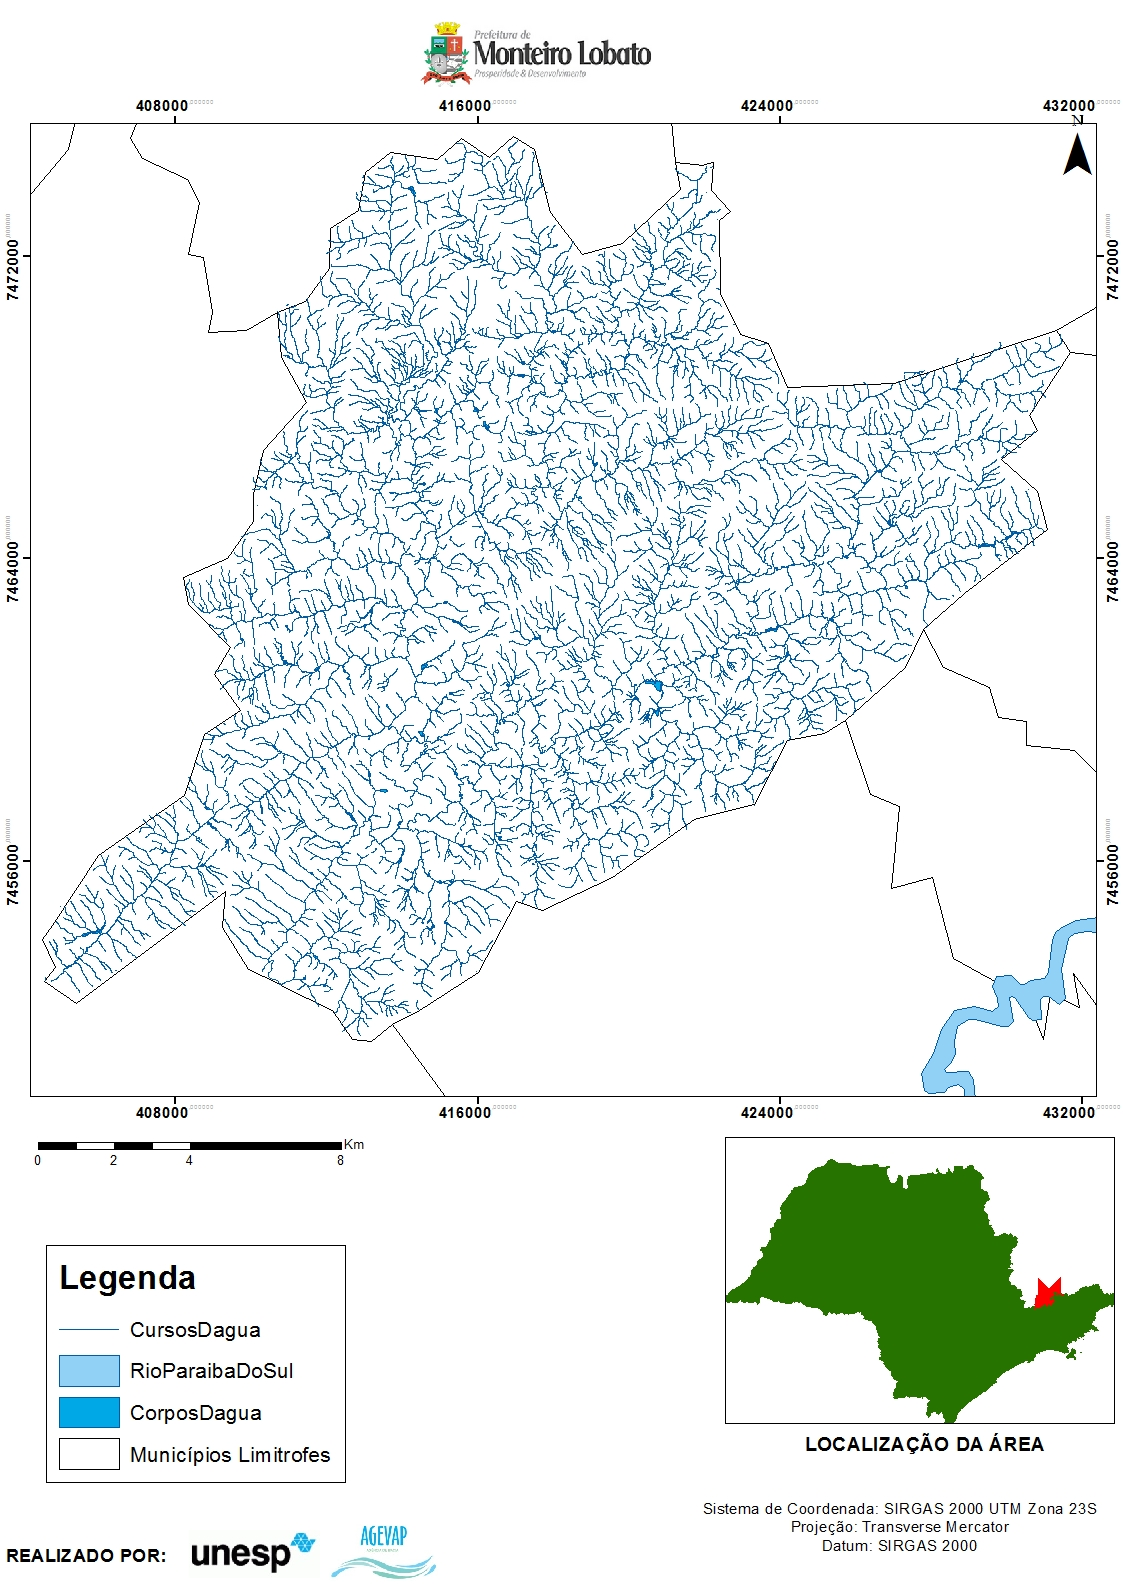
\includegraphics[width=1\linewidth]{produtos/proddois/image022}
 	\caption{Rede de drenagem do município de Monteiro Lobato -SP.}
 	\legend{Fonte: Adaptado IPT, 2016.}
 	\label{fig:image022}
 \end{figure}
\clearpage

\section{Organização territorial e político-administrativa}
\subsection{Organização territorial}
\subsubsection{Distritos e Bairros}

No município de Monteiro Lobato não há formação de distritos, possuindo 19 bairros distribuídos por seu território, e listado conforme na \autoref{tab:bairros}.

	% Table generated by Excel2LaTeX from sheet 'bairros_monteiro'
\begin{table}[htbp]
  \centering
  \arrayrulecolor[rgb]{ 1, 1, 1}
  \caption{Bairros de Monteiro Lobato.}
    \begin{tabular}{c|c}
    \rowcolor[rgb]{ .984,  .831,  .706} Bairro do Souza & Bairro da Matinada \\
    \rowcolor[rgb]{ .992,  .914,  .851} Centro & Bairro Pedra Branca \\
    \rowcolor[rgb]{ .984,  .831,  .706} Vila São Sebastião & Bairro da Serrinha \\
    \rowcolor[rgb]{ .992,  .914,  .851} Vila Esperança & Bairro dos Teixeiras \\
    \rowcolor[rgb]{ .984,  .831,  .706} Vargem Alegre & Bairro Ponte Nova \\
    \rowcolor[rgb]{ .992,  .914,  .851} Bairro São Benedito & Bairro do Turvo \\
    \rowcolor[rgb]{ .984,  .831,  .706} Bairro Descoberto & Bairro dos Forros \\
    \rowcolor[rgb]{ .992,  .914,  .851} Jardim Morada do Sol & São Gotardo \\
    \rowcolor[rgb]{ .984,  .831,  .706} Bairro Alpes do Buquira & Bairro Brumado \\
    \rowcolor[rgb]{ .992,  .914,  .851} Bairro Taquari & Bairro Ferreiras \\
    \end{tabular}%
  \label{tab:bairros}%
\end{table}%


\subsection{Organização Político Administrativa}
O Poder Executivo dentro dos limites do município é exercido pelo Prefeito, cujo gabinete está atualmente estruturado conforme a \autoref{tab:gabinete}. A prefeita, primeira mulher a exercer tal cargo, foi eleita em 2012 para exercício em 2013 e reeleita em 2016 para novo exercícios.

	% Table generated by Excel2LaTeX from sheet 'gabinete'
\begin{table}[htbp]
  \centering
  \arrayrulecolor{white}
  \caption{Gabinete da Prefeitura de Monteiro Lobato.}
    \begin{tabular}{P{0.2\textwidth} P{0.4\textwidth} P{0.1\textwidth}}
    \rowcolor[rgb]{ .969,  .588,  .275} 
    \multicolumn{1}{P{0.2\textwidth}}{\textcolor[rgb]{ 1,  1,  1}{\textbf{Cargo}}} & \multicolumn{1}{P{0.4\textwidth}}{\textcolor[rgb]{ 1,  1,  1}{\textbf{Nome do responsável}}} & \textcolor[rgb]{ 1,  1,  1}{\textbf{Partido}} \\
    \rowcolor[rgb]{ .992,  .914,  .851} Prefeita & Daniela de Cássia Santos Brito & PSB \\
    \rowcolor[rgb]{ .984,  .831,  .706} Vice-Prefeito & Vicente de Paula Prisco da Cunha & PSDB \\
    \end{tabular}%
  \label{tab:gabinete}%
\end{table}%



O gabinete é auxiliado pelos Secretários Municipais, os quais são divididos em 9 secretarias, como mostra a \autoref{tab:secretarias} com seus respectivos representantes. A Secretaria Municipal de Administração é o órgão da estrutura organizacional da Prefeitura incumbido de desempenhar atividades pertinentes às áreas de recursos humanos, compras e licitações, segurança do trabalho, tecnologia da informação e protocolo (abertura e acompanhamento de processos) ~\cite{MonteiroLobatoSite}.

A Secretaria de Cultura e Turismo planeja e coordena o apoio e a execução de atividades para a difusão e formação cultural, bem como a valorização das raízes culturais da população e o desenvolvimento da cidadania no município de Monteiro Lobato. A Secretaria de Cultura e Turismo é responsável pela organização das festas tradicionais e dos eventos de caráter cultural do município lobatense ~\cite{MonteiroLobatoSite}.

A Secretaria Municipal de Desenvolvimento Social de Monteiro Lobato tem por objetivo formular, implantar, financiar, executar, monitorar e avaliar a Política Municipal de Assistência Social, como parte integrante do Sistema Único de Assistência Social (SUAS). As políticas públicas implantadas na Secretaria visam prestar o atendimento integral às famílias, as crianças e aos adolescentes, as mulheres, aos idosos e as pessoas portadoras de necessidades especiais, sendo que a maior prioridade são os segmentos em situação de maior vulnerabilidade social ~\cite{MonteiroLobatoSite}.
A Secretaria Municipal de Educação tem como objetivo principal trabalhar com a ideia de Inclusão em todos os níveis, integrando cooperativamente todas as escolas do município, sejam elas municipais, estaduais ou privadas ~\cite{MonteiroLobatoSite}.

A Secretaria de Esportes e Lazer trabalha para oferecer à população opções nas áreas de esportes e entretenimento, de forma gratuita. Além disso, fomenta as atividades de competição envolvendo os moradores de Monteiro Lobato, principalmente a juventude ~\cite{MonteiroLobatoSite}.

A Secretaria de Finanças e Tributação desenvolve as atividades governamentais superiores de condução dos negócios da fazenda pública municipal, em atendimento às diretrizes traçadas pelo chefe do executivo e as atividades administrativas, objetivando a concretização das decisões políticas, principalmente, mas não só apenas, no que tange a elaboração do PPA (Plano Plurianual), da LDO (Lei de Diretrizes Orçamentárias) e da LOA (Lei Orçamentária Anual), isso com o auxílio das demais secretarias e órgãos da Administração Pública, bem como ao que se refere ao planejamento orçamentário, à execução orçamentária, à realização de receitas, a efetivação das despesas, a movimentação financeira e a administração tributária ~\cite{MonteiroLobatoSite}.

É de competência básica da Secretaria Municipal Meio Ambiente e Agricultura o planejamento, apoio e desenvolvimento de políticas públicas para o setor agropecuário e para a conservação e proteção do meio ambiente. Atua no setor de Meio Ambiente, cujo objetivo é gerenciar o ambiente local buscando diminuição de impactos negativos para todas as formas de vida e a conservação dos recursos naturais; e no setor de Agricultura, com o objetivo de incentivar e promover atividades ligadas à agricultura e à pecuária ~\cite{MonteiroLobatoSite}.

O serviço de saúde, de responsabilidade integral da Secretaria Municipal de Saúde, preza pelo bom atendimento dentro das normas preconizadas pelo SUS e objetiva acolher para cuidar, trabalhando na prevenção de doenças e agravos, visando o bem-estar e qualidade de vida das pessoas. Conta com atendimento na zona urbana e nos bairros da zona rural, com duas equipes compostas com médico, enfermeira, auxiliar de enfermagem e agente comunitário de saúde ~\cite{MonteiroLobatoSite}.

Já a Secretaria Municipal de Transportes tem a função de manter as estradas rurais em boas condições de tráfego. O município tem quase 400 km de estradas que levam a diversos bairros na zona rural. Este cuidado se justifica pela vocação rural de Monteiro Lobato, o que exige estradas bem cuidadas para facilitar o transporte de produtos agropecuários, especialmente a produção de leite ~\cite{MonteiroLobatoSite}.

% Table generated by Excel2LaTeX from sheet 'secretarias'
\begin{table}[htbp]
	\centering
	\caption{Secretarias Municipais de Monteiro Lobato.}
	\begin{tabular}{c|c}
		\rowcolor[rgb]{ .969,  .588,  .275} \textcolor[rgb]{ 1,  1,  1}{\textbf{Divisão}} & \textcolor[rgb]{ 1,  1,  1}{\textbf{Nome do responsável}} \\
		\rowcolor[rgb]{ .992,  .914,  .851} Administração & Priscila Maria Medeiros Dias Magalhães \\
		\rowcolor[rgb]{ .984,  .831,  .706} Cultura e Turismo & Mariana Santos \\
		\rowcolor[rgb]{ .992,  .914,  .851} Desenvolvimento Social & Alexandre Nunes Barbedo \\
		\rowcolor[rgb]{ .984,  .831,  .706} Educação & Ellen Denise Dias da Silva Veloso Bertolini \\
		\rowcolor[rgb]{ .992,  .914,  .851} Esportes e Lazer & Tiago Viana \\
		\rowcolor[rgb]{ .984,  .831,  .706} Finanças e Tributação & Nayane Larissa Rocha Silva \\
		\rowcolor[rgb]{ .992,  .914,  .851} Meio Ambiente e Agricultura & Pedro Luiz de Souza Morais \\
		\rowcolor[rgb]{ .984,  .831,  .706} Saúde & Cláudia Mara Darrigo \\
		\rowcolor[rgb]{ .992,  .914,  .851} Transportes e Serviços Gerais & Aluani Sene \\
	\end{tabular}%
	\label{tab:secretarias}%
\end{table}%


\subsubsection{Poder Legislativo}
O Poder Legislativo é exercido pela Câmara dos Vereadores, e é composta em Monteiro Lobato por 9 vereadores, como previsto para Municípios de até 15.000 (quinze mil) habitantes – no Capítulo IV, artigo 29 da Constituição Federal de 1988. A Mesa Diretora é composta pelo Presidente, Vice-Presidente, Primeiro Secretário e Segundo Secretário.

De acordo com o Artigo 21 do Regimento Interno da Câmara Municipal de Monteiro Lobato, o Presidente é o representante legal da Câmara em suas relações externas, cabendo-lhe as funções administrativas de todas as atividades internas, competindo-lhe privativamente as atividades legislativas e a administração das sessões. Ao Primeiro Secretário, cabe constar a presença dos vereadores, assinar (conjuntamente com o Presidente) todas as Atas aprovadas, redigir as Atas das deliberações secretas e auxiliar a Presidência.

Para suprir a falta ou impedimento do Presidente e do Secretário, haverá um Vice-Presidente e um Segundo Secretário, eleitos conjuntamente com aqueles. A formação atual da Mesa Diretora e os demais vereadores encontra-se na \autoref{tab:mesa}, em conjunto com os seus respectivos partidos de posição.

% Table generated by Excel2LaTeX from sheet 'mesa_diretora'
\begin{table}[htbp]
	\centering
	\caption{Câmara Municipal - Mesa Diretora e Vereadores de Monteiro Lobato 2019.}
	\begin{tabular}{P{3cm}P{5cm}P{3cm}}
		\rowcolor[rgb]{ .969,  .588,  .275} 
		\multicolumn{1}{P{3cm}}{\textcolor[rgb]{ 1,  1,  1}{\textbf{Cargo}}} & \multicolumn{1}{P{5cm}}{\textcolor[rgb]{ 1,  1,  1}{\textbf{Nome do responsável}}} & \textcolor[rgb]{ 1,  1,  1}{\textbf{Partido}} \\
		\rowcolor[rgb]{ .992,  .914,  .851} 
		\multicolumn{1}{P{3cm}}{Presidente da Câmara} & Carlos Renato Prince & PV \\
		\rowcolor[rgb]{ .984,  .831,  .706} 
		\multicolumn{1}{P{3cm}}{Vice-presidente} & Ailton Rodolfo Martins & PR \\
		\rowcolor[rgb]{ .992,  .914,  .851} 
		\multicolumn{1}{P{3cm}}{Primeira Secretária} & Luis Carlos Diniz & PV \\
		\rowcolor[rgb]{ .984,  .831,  .706} 
		\multicolumn{1}{P{3cm}}{Segundo Secretário} & João Cunha Francisco da Silva & PV \\
		\rowcolor[rgb]{ .992,  .914,  .851} 
		\multicolumn{1}{c}{\multirow{5}{*}{Vereadores}} & Gislene Aparecida Barreto Costa & PSB \\
		\rowcolor[rgb]{ .992,  .914,  .851}       & Jesse Marcos de Azevedo & PV \\
		\rowcolor[rgb]{ .992,  .914,  .851}       & Odair José de Araújo & DEM \\
		\rowcolor[rgb]{ .992,  .914,  .851}       & José Donizeti Pereira & PTB \\
		\rowcolor[rgb]{ .992,  .914,  .851}       & Odair José Rocha & PMDB \\
	\end{tabular}%
	\label{tab:mesa}%
\end{table}%

\subsection{Dispositivos legais de zoneamento urbano, disciplinadores do uso e ocupação do solo}
O Plano Diretor é uma lei municipal que estabelece diretrizes para a ocupação da cidade, estabelece as exigências fundamentais de ordenamento da Cidade com o principal objetivo de programar o pleno desenvolvimento de suas funções sociais e garantir o bem-estar de seus habitantes. É instrumento básico e estratégico de desenvolvimento do Município, com ênfase na estruturação do seu território.
No Município de Monteiro Lobato, o Plano Diretor é dado pela Lei Nº 1.650 de 15 de setembro de 2017, na qual são estabelecidas definições importantes que discorrem sobre o ordenamento no município. A referida lei define os usos e atividades geradoras de incômodo ou de impacto à vizinhança e estabelece critérios para análise do grau de incomodidade no Artigo 40, entre eles, poluição sonora, atmosférica, por resíduos líquidos, por resíduos sólidos, vibração e periculosidade.

Em relação aos Recursos Hídricos, algumas ações são definidas no Artigo 67, como: executar programas integrados de saneamento ambiental buscando evitar o desperdício e a degradação de mananciais; implementar instrumentos de Avaliação Ambiental para fins de avaliação, monitoramento e revisão de políticas que ameacem a produção de água; instituir o Programa de Recuperação Ambiental de Cursos D’água e Fundos de Vale, sob a coordenação do Executivo e com a participação da sociedade civil, buscando a melhoria da qualidade ambiental da cidade.

As ações definidas para a gestão dos resíduos sólidos estão definidas no Artigo 77, dentre as quais: implementar o tratamento e a disposição ambientalmente adequados dos resíduos remanescentes; controlar a disposição inadequada de resíduos por meio de ações de educação ambiental, oferta de instalações para disposição de resíduos sólidos e fiscalização efetiva; estabelecer nova base legal relativa a resíduos sólidos, disciplinando os fluxos dos diferentes resíduos e os diferentes fatores em consonância com a Política Municipal de Resíduos Sólidos prevista no artigo anterior citado porém, ainda não  legislada.

O Macrozoneamento do Município fixa as regras fundamentais de ordenamento do território, definindo as áreas adensáveis e não adensáveis, de acordo com a capacidade de infraestrutura e preservação do meio ambiente. Para Monteiro Lobato, foram instituídas três Macrozonas: a Urbana, a de Ocupação Controlada e a Rural; as quais são subdivididas no Título IX do Plano Diretor, a fim de contemplar as especificidades de ocupação e dinâmica territorial.

O uso e ocupação do solo no Município de Monteiro Lobato é representado na \autoref{fig:image023}. Há a presença de chácara, cultura temporária, espelho d’água, mineração e reflorestamento. Existem dois pontos principais de área urbanizada no município, localizados mais na parte oeste, sendo um superior e outro inferior, denominados como os bairros de São Benedito e Centro, respectivamente. Há como uso dominante a presença de mata e campo antrópico/pastagem no limite do município.

O Plano Diretor também trata de outras frentes de cunho público, tais como o desenvolvimento e a paisagem urbana e rural, um Plano Municipal de Habitação, da circulação viária e transportes, do patrimônio histórico e cultural, da infraestrutura e serviços de utilidade pública, da pavimentação, da energia e iluminação pública e da rede viária.

\newpage
 \begin{figure}[h!]
	\centering
	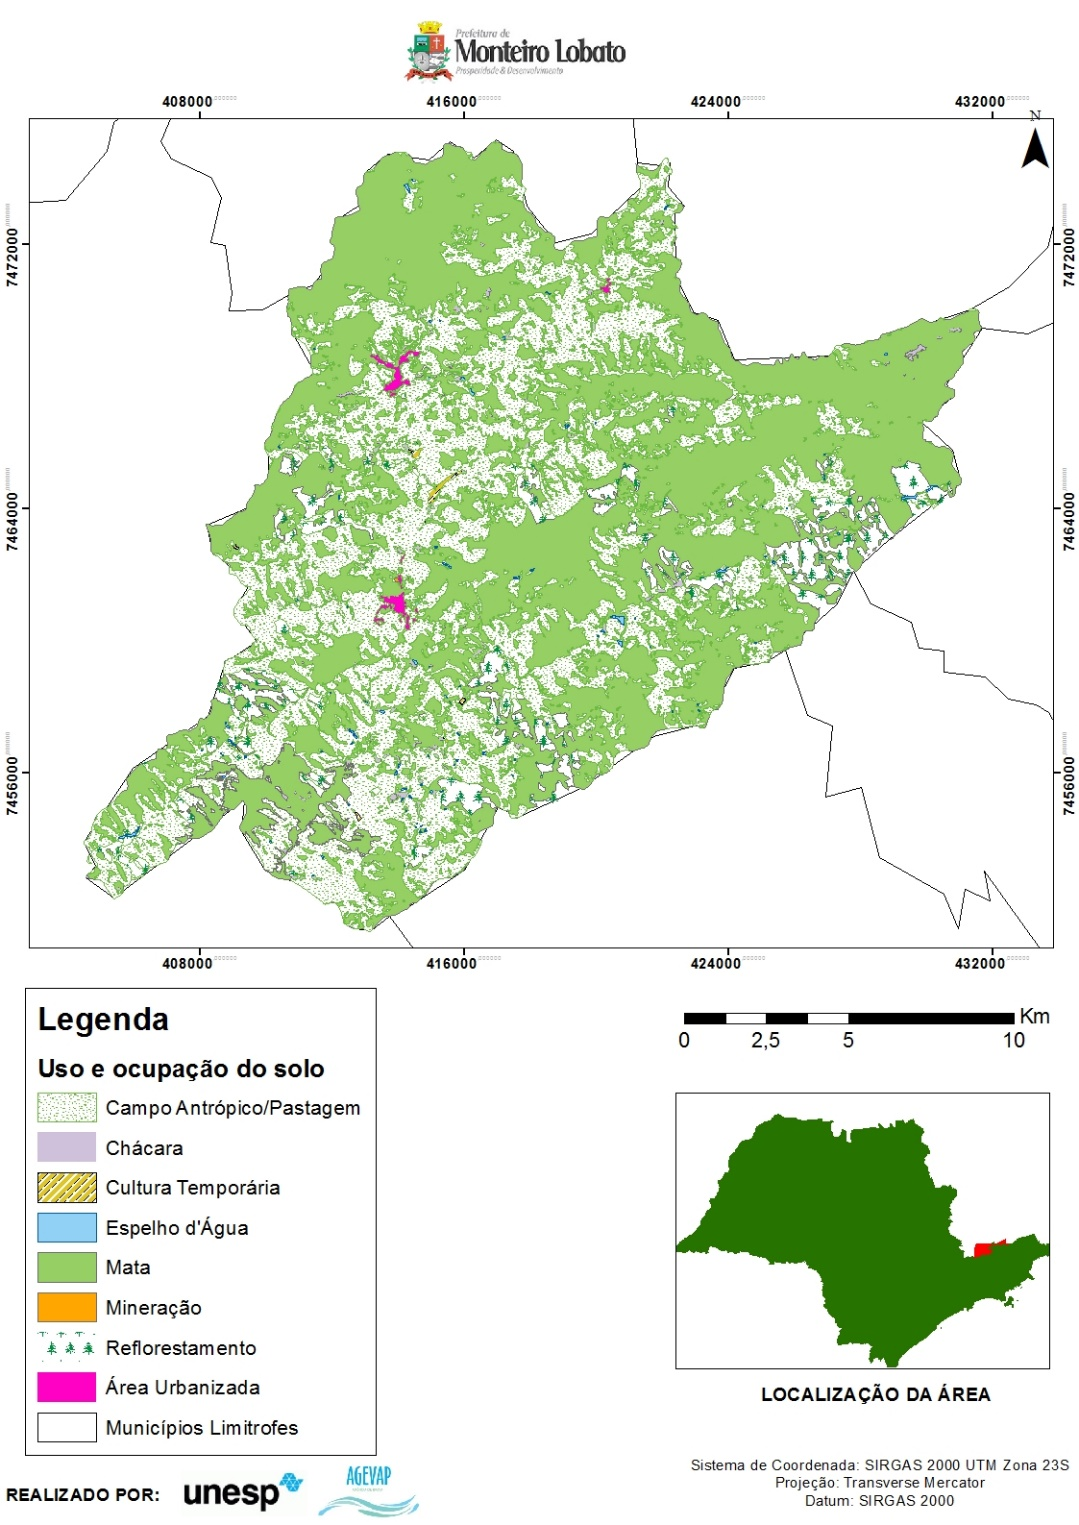
\includegraphics[width=1\linewidth]{produtos/proddois/image023}
	\caption{Uso e ocupação do solo de Monteiro Lobato.}
	\legend{Fonte: Adaptado IPT, 2016.}
	\label{fig:image023}
\end{figure}
\clearpage

\subsection{Demografia}
Segundo dados do SEADE (Fundação Sistema Estadual de Análise de Dados), em seu portal de Informações sobre Municípios Paulistas (IMP), a população do município de Monteiro Lobato vem crescendo de forma lenta indo de uma população de 2682 habitantes na década de 80 para 4431 habitantes atualmente. O município tem um grau de urbanização de 44,28\%, o que indica que a população está dividida quase que igualmente entre população urbana e rural, conforme é possível visualizar na \autoref{fig:image024}. 

 \begin{figure}[h!]
	\centering
	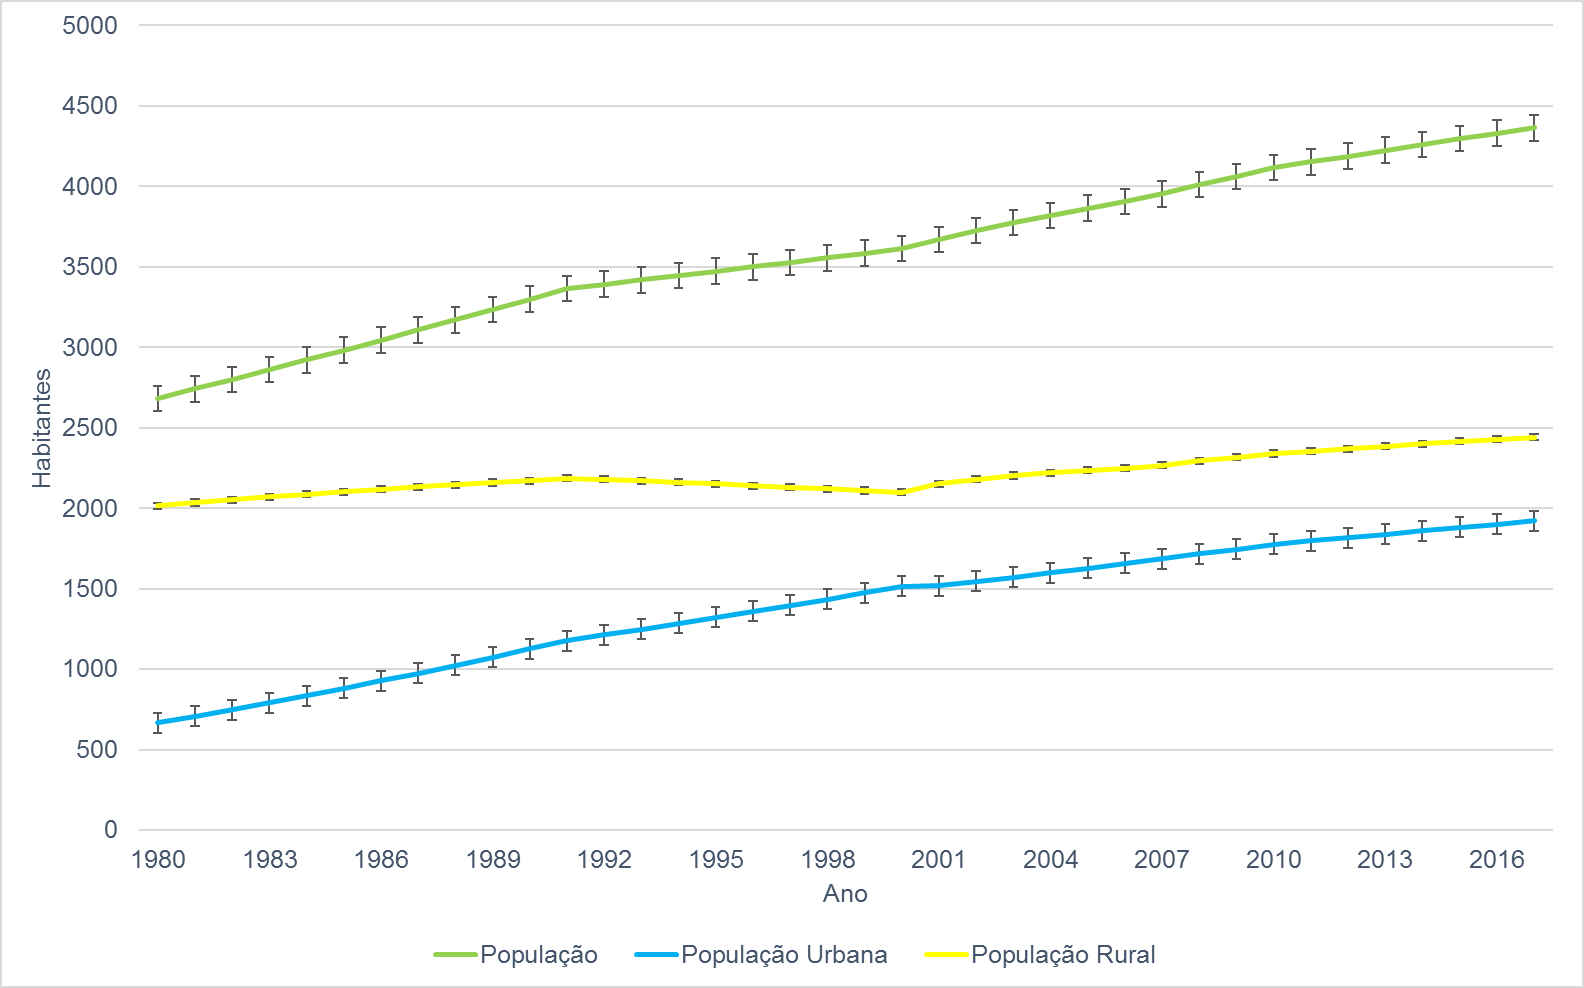
\includegraphics[width=0.85\linewidth]{produtos/proddois/image024}
	\caption{Série histórica da evolução da população absoluta, urbana e rural do município de Monteiro Lobato durante o período de 1980 a 2017.}
	\legend{Fonte: IMP SEADE, 2017.}
	\label{fig:image024}
\end{figure}

Durante os períodos avaliado as taxas de crescimento da população de Monteiro Lobato flutuam, tem seu maior crescimento entre 1980 – 1991 e o menor entre 1991 – 2000. A \autoref{tab:cresc_pop} demonstra como ocorre a variação das taxas de acordo com os períodos.

% Table generated by Excel2LaTeX from sheet 'cresc_pop'
\begin{table}[htbp]
	\centering
	\caption{Taxa geométrica de crescimento populacional do município de Monteiro Lobato, durante o período de 1980 a 2019.}
	\begin{tabular}{P{2cm}ccc}
		\rowcolor[rgb]{ .969,  .588,  .275} 
		\multicolumn{1}{P{2cm}}{\textcolor[rgb]{ 1,  1,  1}{\textbf{Período}}} & \multicolumn{1}{P{1,7cm}}{\textcolor[rgb]{ 1,  1,  1}{\textbf{População (\% a.a.)}}} & \multicolumn{1}{P{3cm}}{\textcolor[rgb]{ 1,  1,  1}{\textbf{População Urbana (\% a.a.)}}} & \multicolumn{1}{P{2,5cm}}{\textcolor[rgb]{ 1,  1,  1}{\textbf{População Rural (\% a.a.)}}} \\
		\rowcolor[rgb]{ .992,  .914,  .851} 1980-1991 & 2,08  & 5,3   & 0,75 \\
		\rowcolor[rgb]{ .984,  .831,  .706} 1991-2000 & 0,8   & 2,84  & -0,46 \\
		\rowcolor[rgb]{ .992,  .914,  .851} 2000-2010 & 1,31  & 1,61  & 1,09 \\
		\rowcolor[rgb]{ .984,  .831,  .706} 2010-2019 & 0,82  & 1,11  & 0,6 \\
	\end{tabular}%
	\label{tab:cresc_pop}%
\end{table}%

A pirâmide etária demonstra a distribuição da população por faixa etária. Por meio de dados do Censo Demográfico de 2010, realizado pelo IBGE, foi elaborada a pirâmide etária por gênero para o município de Monteiro Lobato ilustrada na \autoref{fig:image025}. O município apresenta uma maior proporção de pessoas na base da pirâmide em relação aos outros dois municípios.


\begin{figure}[h!]
 	\centering
 	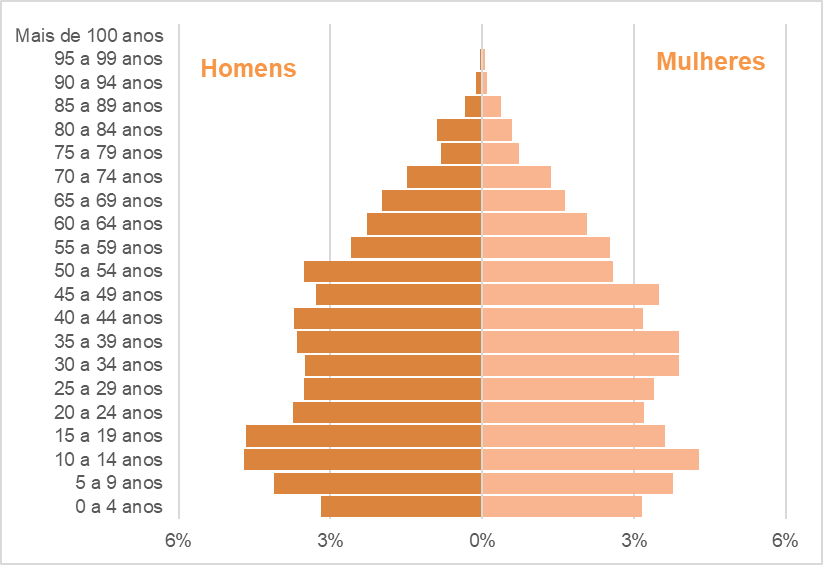
\includegraphics[width=0.85\linewidth]{produtos/proddois/image025}
 	\caption{Pirâmide Etária de Monteiro Lobato – 2010.}
 	\legend{Fonte: IBGE, 2010.}
 	\label{fig:image025}
 \end{figure}

Os intervalos de idade de 10 a 54 anos não há um padrão de natalidade bem definido, com acréscimos e decréscimos na taxa de natalidade. O mesmo comportamento da pirâmide etária do município de Monteiro Lobato pode ser observado na \autoref{fig:image026} abaixo, que é uma projeção para 2017 realizada pelo IMP,

  \newpage
  \clearpage
  \begin{figure}[h!]
 	\centering
 	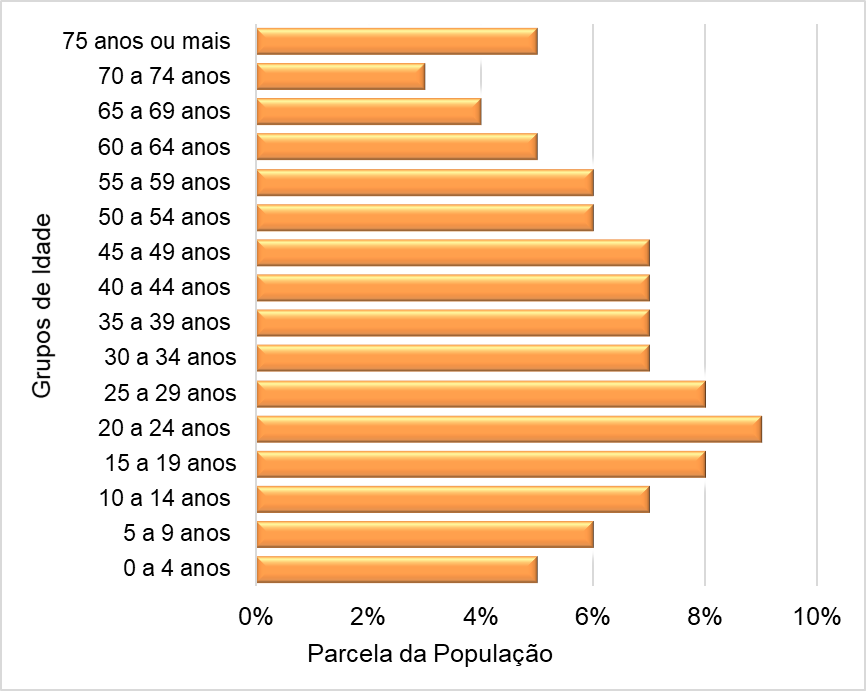
\includegraphics[width=0.8\linewidth]{produtos/proddois/image026}
 	\caption{População de Monteiro Lobato por Grupos de Idade – 2017.}
 	\legend{Fonte: IMP SEADE, 2017.}
 	\label{fig:image026}
 \end{figure}

\section{Macroinformações socioeconômicas}
\subsection{Educação}

O último Censo Demográfico realizado pelo IBGE em 2010 designou à cidade de Monteiro Lobato uma taxa de escolarização de 96,5\% para crianças entre 6 a 14 anos, o que demonstra que quase a totalidade da população desta faixa etária está matriculada em alguma etapa do ensino fundamental. Apesar da alta taxa de pessoas matriculadas, o município ocupa a posição de 4193º dentre os 5570 da República Federativa Brasil, sendo o 576º de 645 municípios do Estado de São Paulo, e o 4º dos 4 municípios que compõem a microrregião de Campos do Jordão.

Em números absolutos, as matrículas de alunos para o ano de 2015 em Monteiro Lobato foram de 107 inscrições na pré-escola, 721 no ensino fundamental, e 202 no ensino médio. A \autoref{fig:image027} mostra a série histórica de matrículas consolidadas de 2012 a 2016 para diferentes níveis de ensino no município de Monteiro Lobato.

\begin{figure}[h!]
	\centering
	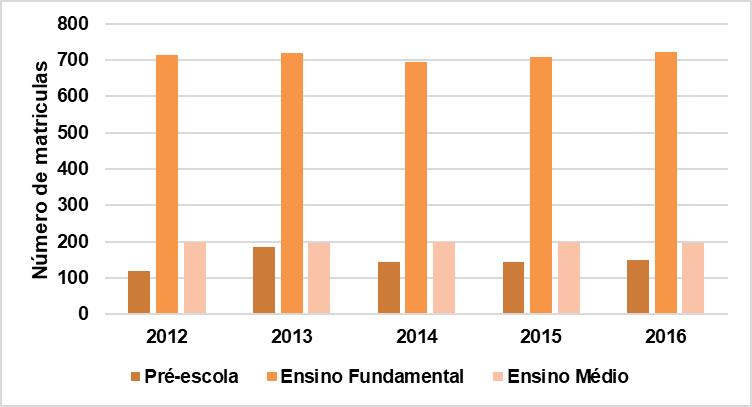
\includegraphics[width=0.8\linewidth]{produtos/proddois/image027}
	\caption{Série histórica de matrículas consolidadas de 2012 a 2016 para diferentes níveis de ensino no município de Monteiro Lobato.}
	\legend{Fonte: IMP SEADE, 2017.}
	\label{fig:image027}
\end{figure}

Dentre as matrículas consolidadas em cada ano para cada nível de ensino, há a possibilidade do aluno ser aprovado, reprovado e de abandonar o curso. As taxas estão ilustradas na \autoref{fig:image028}, \autoref{fig:image029} e \autoref{fig:image030}.

\begin{figure}[h!]
	\centering
	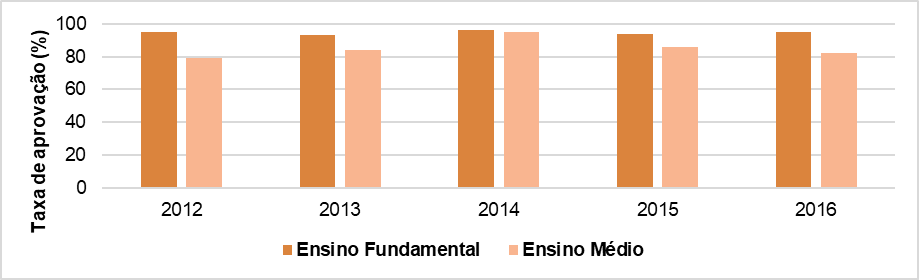
\includegraphics[width=1\linewidth]{produtos/proddois/image028}
	\caption{Série histórica da taxa de aprovação ocorridas de 2012 a 2016 para diferentes níveis de ensino no município de Monteiro Lobato.}
	\label{fig:image028}
\end{figure}

\begin{figure}[h!]
	\centering
	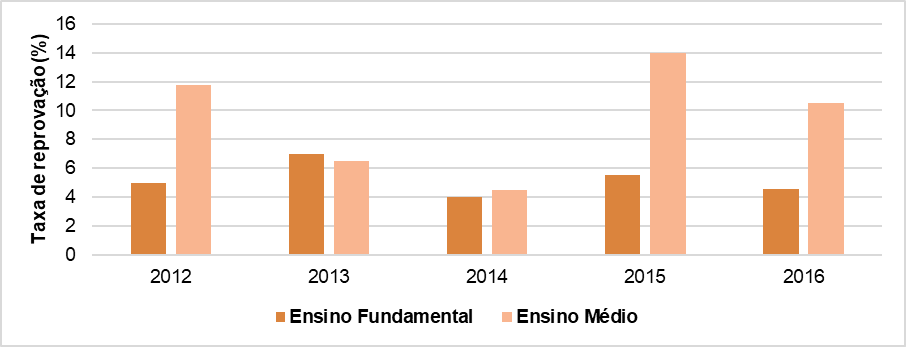
\includegraphics[width=1\linewidth]{produtos/proddois/image029}
	\caption{Série histórica da taxa de reprovação ocorridas de 2012 a 2016 para diferentes níveis de ensino no município de Monteiro Lobato.}
	\legend{Fonte: IMP SEADE, 2017.}
	\label{fig:image029}
\end{figure}

\begin{figure}[h!]
	\centering
	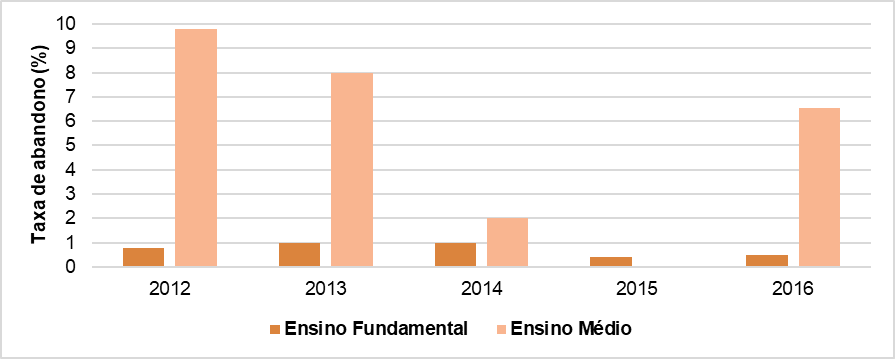
\includegraphics[width=1\linewidth]{produtos/proddois/image030}
	\caption{Série histórica da taxa de abandono ocorridas de 2012 a 2016 para diferentes níveis de ensino no município de Monteiro Lobato.}
	\legend{Fonte: IMP SEADE, 2017.}
	\label{fig:image030}
\end{figure}
\clearpage

As taxas de aprovações dos últimos anos do ensino fundamental e do ensino médio podem ser tratadas em termos absolutos pelo quesito de alunos concluintes, como demonstrado na \autoref{fig:image031}.

\begin{figure}[h!]
	\centering
	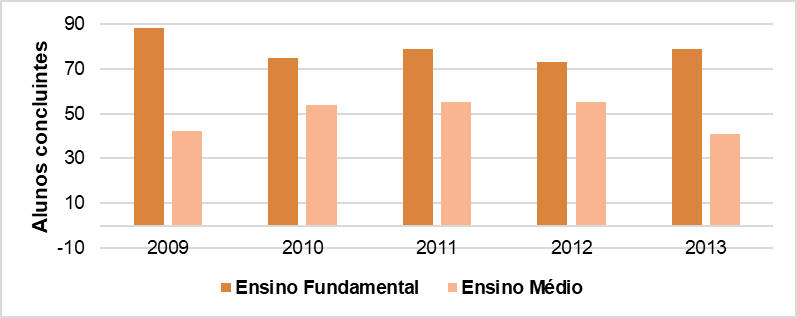
\includegraphics[width=1\linewidth]{produtos/proddois/image031}
	\caption{Série histórica de alunos concluintes de 2012 a 2016 para diferentes níveis de ensino no município de Monteiro Lobato.}
	\legend{Fonte: IMP SEADE, 2017.}
	\label{fig:image031}
\end{figure}

Através do IDEB - Índice de Desenvolvimento de Educação Básica, indicador utilizado para avaliar a qualidade do aprendizado em âmbito nacional e estabelecer metas para a melhoria do ensino, o município de Monteiro Lobato alcançou em 2015 nota média de 6.8 para alunos dos anos iniciais do ensino fundamental, e 4.7 para os alunos dos anos finais da mesma etapa de ensino.

Esse índice para os primeiros anos do ensino básico classifica o município como o 266º de 5570 na perspectiva nacional, 76º de 645 no Estado de São Paulo, e primeiro lugar dentre quatro municípios da microrregião de Campos do Jordão. O cenário da avaliação para os últimos anos do ensino básico indica a posição 1402º de 5570 no âmbito federal, 416 de 645 no estadual, e terceiro de quatro municípios na microrregião de Campos de Jordão.
	
O município de Monteiro Lobato conta com quatro núcleos escolares que atendem à demanda pelos diferentes níveis de ensino. A \autoref{fig:image032} a seguir indica a localização geográfica das escolas, concentradas majoritariamente na região central do município. 
\newpage
\begin{figure}[h!]
 	\centering
 	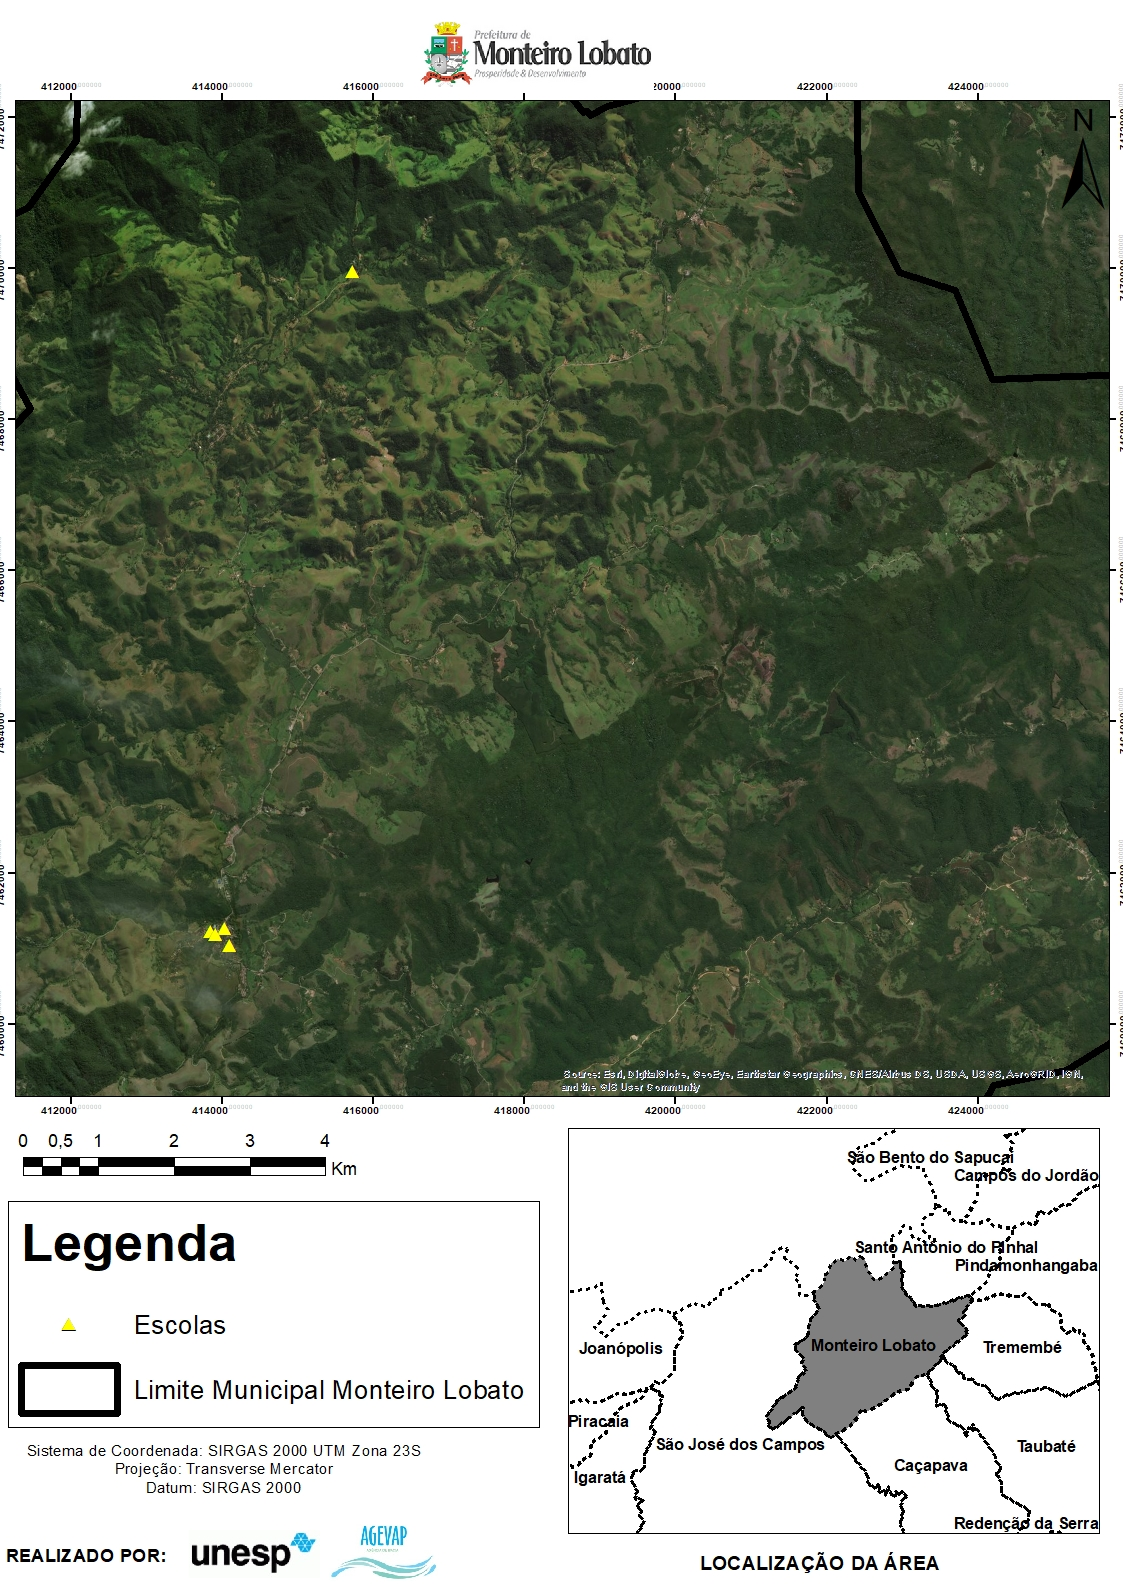
\includegraphics[width=1\linewidth]{produtos/proddois/image032}
 	\caption{Localização geográfica de escolas no município de Monteiro Lobato.}
 	\label{fig:image032}
 \end{figure}
\clearpage
\subsection{Trabalho e renda}

A necessidade de se traçar um perfil de renda para os habitantes do município de Monteiro Lobato se dá pela possibilidade de comparação com outros municípios e assim poder determinar fatores de qualidade de vida em termos monetários. Os dois últimos censos demográficos (2000 e 2010) identificaram a renda per capita dos lobatenses, Na \autoref{fig:image033} segue a ilustração gráfica.

\begin{figure}[h!]
	\centering
	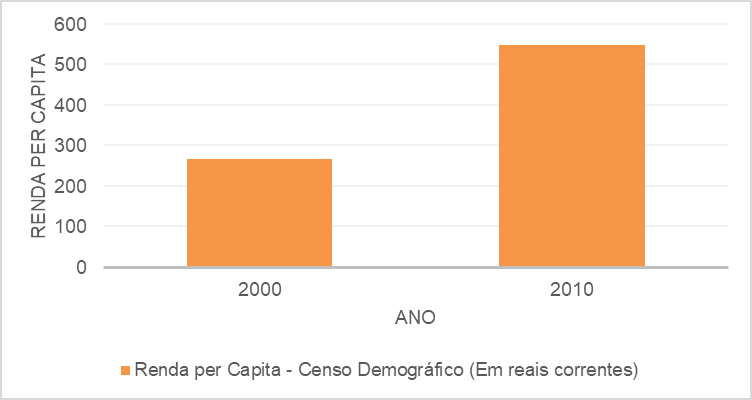
\includegraphics[width=0.75\linewidth]{produtos/proddois/image033}
	\caption{Renda per Capita do município de Monteiro Lobato.}
	\label{fig:image033}
\end{figure}

Para identificar a contribuição de cada setor de atividade econômica com o rendimento total do município de Monteiro Lobato, a seguinte série histórica de rendimento médio de empregos formais por atividade econômica, que compreende os anos de 2011 a 2015, demonstra quais setores designam os melhores salários (\autoref{fig:image034}).
 
 \begin{figure}[h!]
 	\centering
 	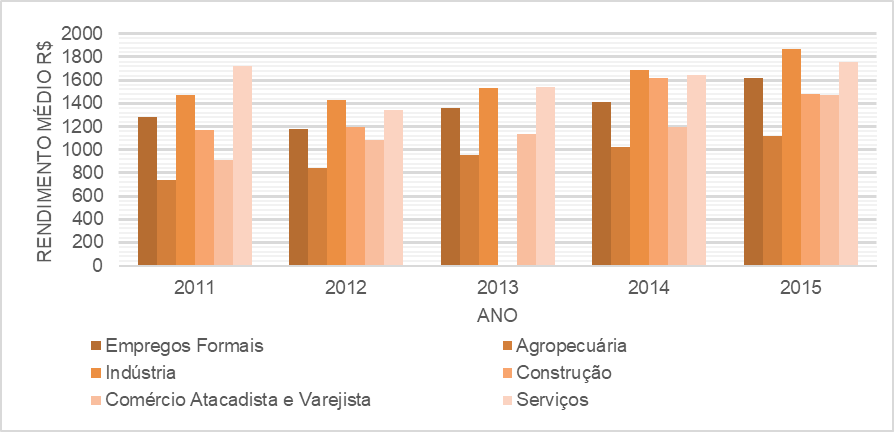
\includegraphics[width=0.8\linewidth]{produtos/proddois/image034}
 	\caption{Rendimento médio dos empregos formais por setores de atividade econômica.}
 	\label{fig:image034}
 \end{figure}

Como informação complementar, tem-se as quantidades absolutas e relativas de empregos por atividade econômica no município de Monteiro Lobato, como representado na \autoref{fig:image035} e \autoref{fig:image036}, respectivamente.
 
 \begin{figure}[h!]
 	\centering
 	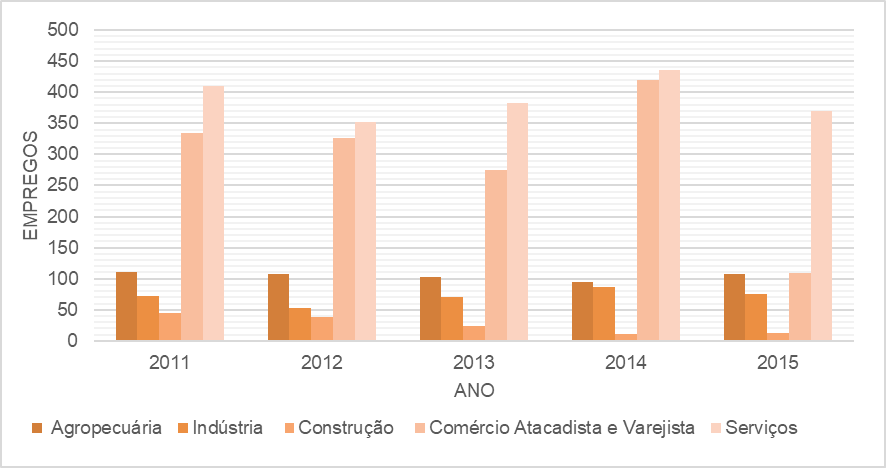
\includegraphics[width=1\linewidth]{produtos/proddois/image035}
 	\caption{Empregos formais por setores de atividade econômica.}
 	\label{fig:image035}
 \end{figure}
 
 \begin{figure}[h!]
 	\centering
 	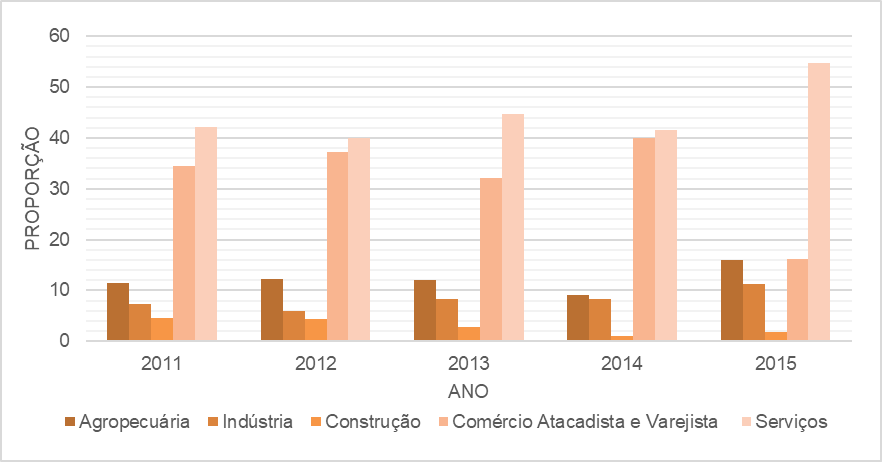
\includegraphics[width=1\linewidth]{produtos/proddois/image036}
 	\caption{Participação dos Empregos Formais por setores de atividade econômica.}
 	\label{fig:image036}
 \end{figure}

\subsection{Indicadores de saúde e estatísticas vitais}

Para entender melhor os resíduos sólidos gerados em Monteiro Lobato e elaborar um planejamento público a médio e longo prazo, é necessário entender as estatísticas vitais do município. A taxa de natalidade bruta é um destes dados, que relaciona a quantidade de indivíduos que nascem em um intervalo definido de tempo. Comumente, essa taxa é indicada em intervalos anuais e em uma proporção a cada mil habitantes da região analisada. 

As figuras (\autoref{fig:image037} e \autoref{fig:image038}) mostram a taxa de natalidade do município de Monteiro Lobato, e do Estado de São Paulo entre os anos de 2011 e 2016.

 \begin{figure}[h!]
	\centering
	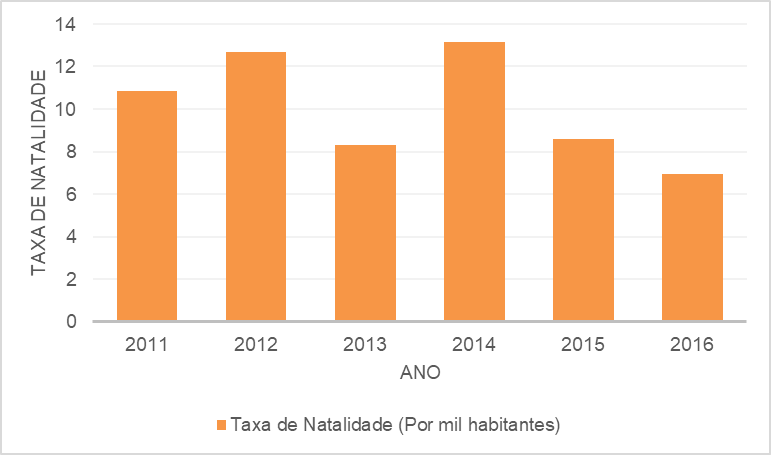
\includegraphics[width=0.9\linewidth]{produtos/proddois/image037}
	\caption{Taxa de natalidade do município de Monteiro Lobato por mil habitantes.}
	\label{fig:image037}
\end{figure}
\newpage
 \begin{figure}[h!]
	\centering
	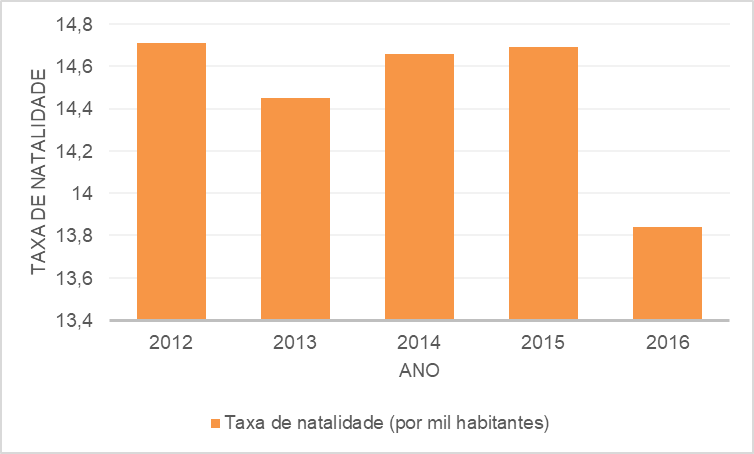
\includegraphics[width=0.9\linewidth]{produtos/proddois/image038}
	\caption{Taxa de natalidade Estado de São Paulo por mil habitantes.}
	\label{fig:image038}
\end{figure}

Como comparação, a média da taxa de natalidade por mil habitantes do município de Monteiro Lobato dos últimos seis anos assume o valor de 10,078; ~\cite{SEADE2017}.

A taxa de mortalidade geral relaciona o número de mortes, expresso por mil habitantes, em um intervalo de tempo definido em um espaço geográfico determinado. O município de Monteiro Lobato e o Estado de São Paulo possuem as séries históricas, demonstradas na \autoref{fig:image039} e \autoref{fig:image040}  entre os anos de 2011 e 2016.

 \begin{figure}[h!]
	\centering
	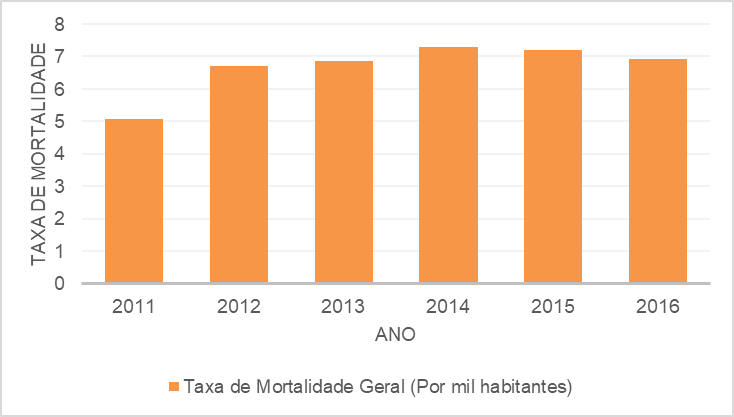
\includegraphics[width=0.9\linewidth]{produtos/proddois/image039}
	\caption{Taxa de mortalidade geral por mil habitantes do município de Monteiro Lobato.}
	\label{fig:image039}
\end{figure}

 \begin{figure}[h!]
	\centering
	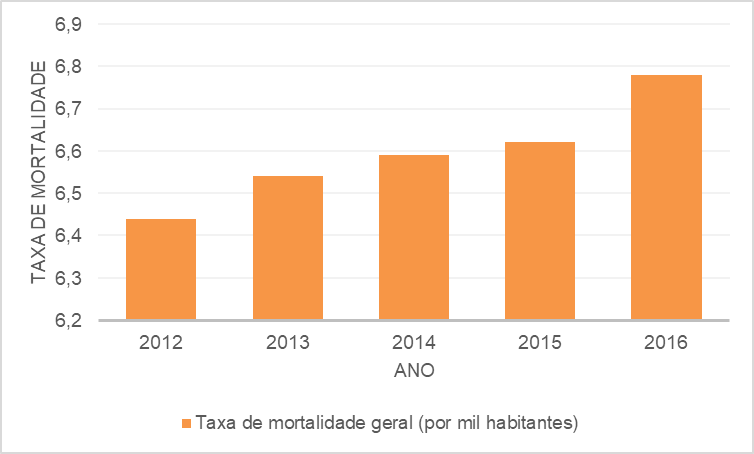
\includegraphics[width=0.9\linewidth]{produtos/proddois/image040}
	\caption{Taxa de mortalidade geral por mil habitantes do Estado de São Paulo.}
	\label{fig:image040}
\end{figure}
\clearpage
Dentro da taxa de mortalidade geral, pode-se identificar a proporção de mortes que foi causada por causas externas, tais como acidentes e violência em geral (por cem mil habitantes); e a taxa de mortalidade infantil, que abrange apenas a população com idade de 0 a 15 anos (por mil habitantes nascidos vivos). Tais gráficos estão representados para regiões específicas, respectivamente para causas externas e taxa de mortalidade infantil, na \autoref{fig:image041},  \autoref{fig:image042}, \autoref{fig:image043} e \autoref{fig:image044}.

 \begin{figure}[h!]
	\centering
	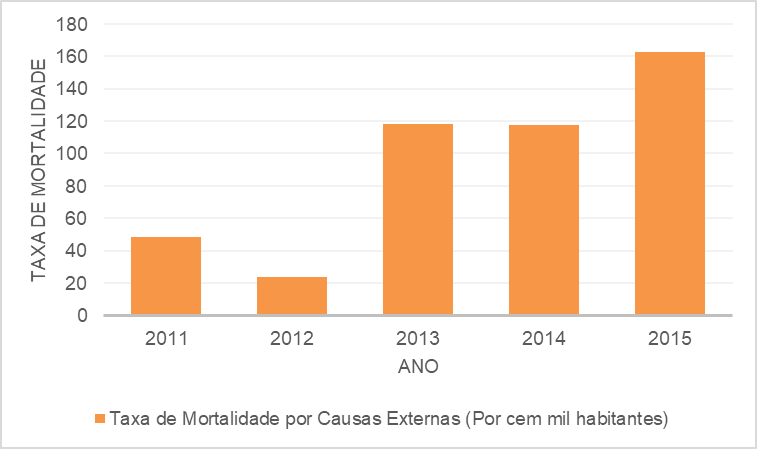
\includegraphics[width=0.75\linewidth]{produtos/proddois/image041}
	\caption{Taxa de mortalidade por causas externas por cem mil habitantes no município de Monteiro Lobato.}
	\label{fig:image041}
\end{figure}

 \begin{figure}[h!]
	\centering
	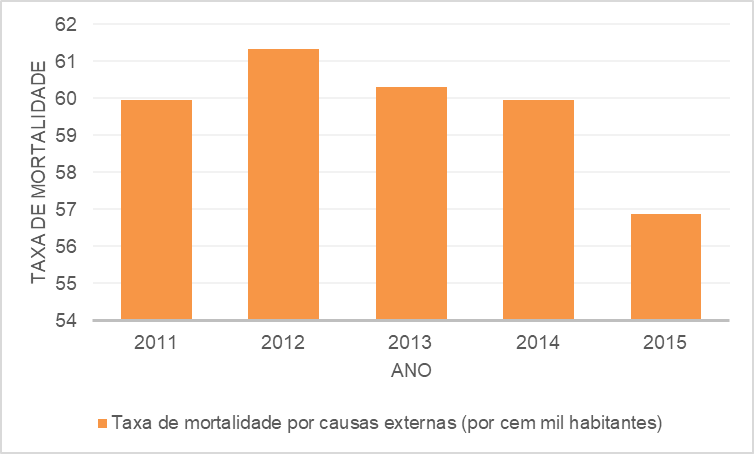
\includegraphics[width=0.75\linewidth]{produtos/proddois/image042}
	\caption{Taxa de mortalidade por causas externas por cem mil habitantes no Estado de São Paulo.}
	\label{fig:image042}
\end{figure}
 \newpage
  \begin{figure}[h!]
 	\centering
 	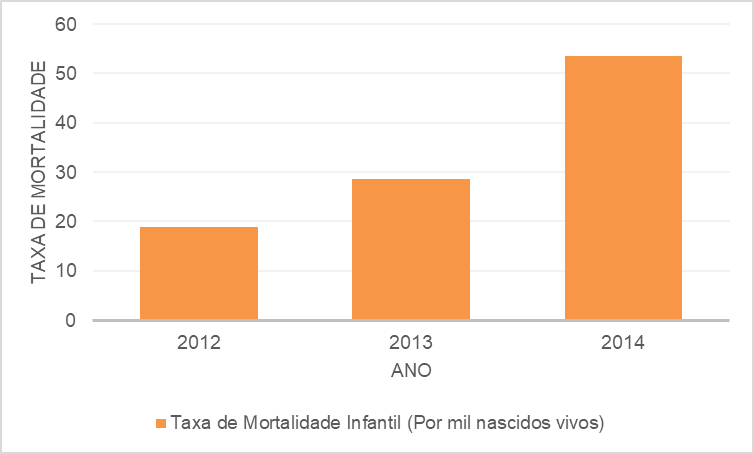
\includegraphics[width=0.75\linewidth]{produtos/proddois/image043}
 	\caption{Taxa de mortalidade infantil por mil nascidos vivos do município de Monteiro Lobato.}
 	\label{fig:image043}
 \end{figure}

 \begin{figure}[h!]
	\centering
	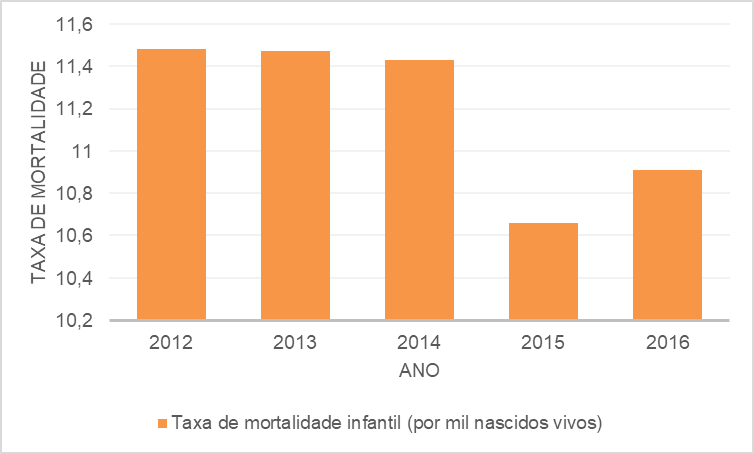
\includegraphics[width=0.75\linewidth]{produtos/proddois/image044}
	\caption{Taxa de mortalidade infantil por mil nascidos vivos do Estado de São Paulo.}
	\label{fig:image044}
\end{figure}

Em termos de taxa de mortalidade geral, a média do município de Monteiro Lobato se deu por 6,67. Já o Estado de São Paulo apresentou média de 11,19.
\clearpage

\subsection{Economia}

Segundo o SEADE (Sistema Estadual de Análise de Dados) em seu portal de Informações sobre Municípios Paulistas (IMP), o Produto Interno Bruto de uma região é um índice que assume o valor monetário da soma de todos os bens e serviços produzidos durante um período de tempo definido, medindo assim a atividade econômica da região, e possibilitando sua classificação e comparação com diferentes períodos e também unidades territoriais. A \autoref{fig:image045} ilustra a série histórica do Produto Interno Bruto do município de Monteiro Lobato entre os anos de 2010 a 2014.

 \begin{figure}[h!]
	\centering
	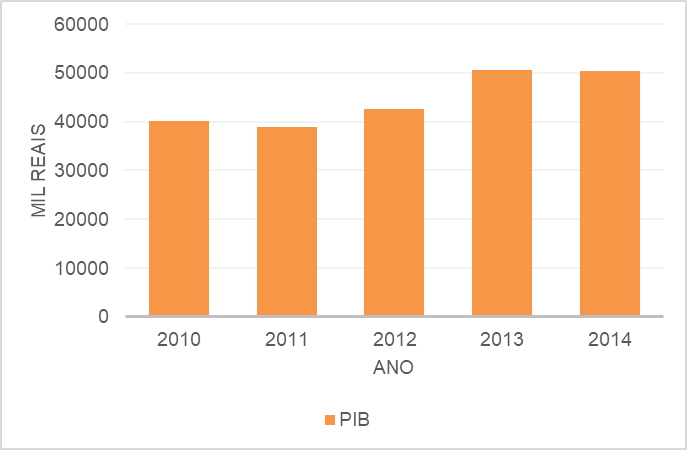
\includegraphics[width=0.8\linewidth]{produtos/proddois/image045}
	\caption{Série histórica do Produto Interno Bruto do município de Monteiro Lobato entre os anos de 2010 a 2014.}
	\legend{Fonte: IMP SEADE, 2017.}
	\label{fig:image045}
\end{figure}

Derivado do PIB, o PIB per capita é o índice que representa a totalidade dos bens e serviços produzidos em cifras monetárias dividida pela quantidade de habitantes da região. Ao fazer a relação entre valor produzido e quantidade de habitantes, o PIB per capita torna-se um índice mais concreto para analisar e qualificar a qualidade de vida da população de determinada área baseado na atividade econômica lá desenvolvida. A \autoref{fig:image046} apresenta a série histórica do PIB per capta do município de Monteiro Lobato entre os anos de 2010 a 2014.

 \begin{figure}[h!]
	\centering
	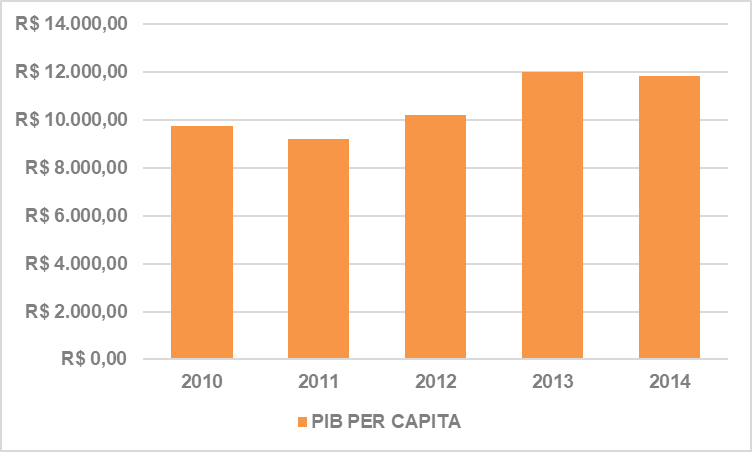
\includegraphics[width=0.75\linewidth]{produtos/proddois/image046}
	\caption{Série histórica do Produto Interno Bruto do município de Monteiro Lobato entre os anos de 2010 a 2014.}
	\legend{Fonte: IMP SEADE, 2017.}
	\label{fig:image046}
\end{figure}

Ainda há a relação de contribuição de cada setor da economia com o PIB, sendo eles as áreas de administração pública, que engloba as prefeituras, secretarias, câmara dos vereadores, e outros órgãos públicos; o complexo industrial, que abrange as unidades fabris e a infraestrutura destinada para a produção de bens industriais; as atividades agropecuárias, em que estão contidas regiões de fazendas e a logística de transporte; o ramo de serviços em geral, que suporta o comércio urbano, e os impostos sobre produto líquido.

Os impostos sobre produto líquido são a soma dos impostos federais indiretos que estão embutidos no preço dos bens e serviços, mas que não ficam retidos nos agentes econômicos do município, como por exemplo o Imposto sobre Produtos Industrializados (IPI), o Imposto de Importação (II), Impostos sobre Operação de Crédito, Câmbio e Seguro (IOF), Contribuição para o Financiamento da Seguridade Social (COFINS) e Imposto sobre Serviços (ISS).

Dessa forma, a participação de cada setor no PIB do município de Monteiro Lobato pode ser analisada na seguinte série histórica que compreende o intervalo do ano de 2010 até o ano de 2014 ilustrada pela \autoref{fig:image047}.

  \begin{figure}[h!]
 	\centering
 	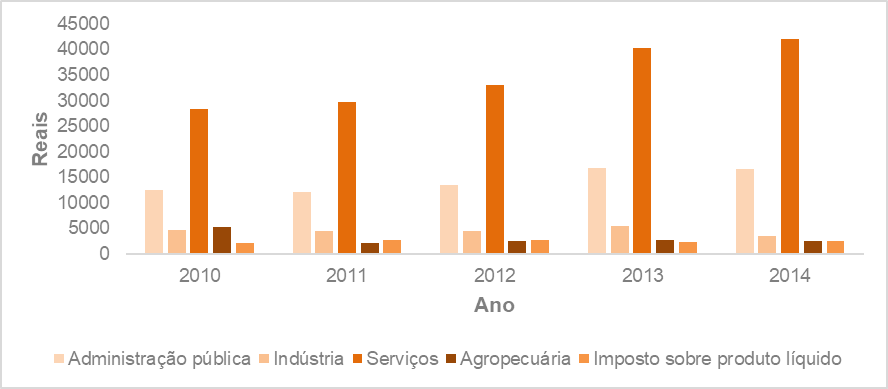
\includegraphics[width=0.85\linewidth]{produtos/proddois/image047}
 	\caption{Série histórica da participação de cada setor no PIB do município de Monteiro Lobato entre os anos de 2010 a 2014.}
 	\legend{Fonte: IMP SEADE, 2017.}
 	\label{fig:image047}
 \end{figure}

Para melhor visualização da contribuição de cada setor econômico no PIB, construiu-se o gráfico da \autoref{fig:image048} de linhas sobre a participação dos diferentes setores da economia no PIB para o município de Monteiro Lobato.

 \begin{figure}[h!]
	\centering
	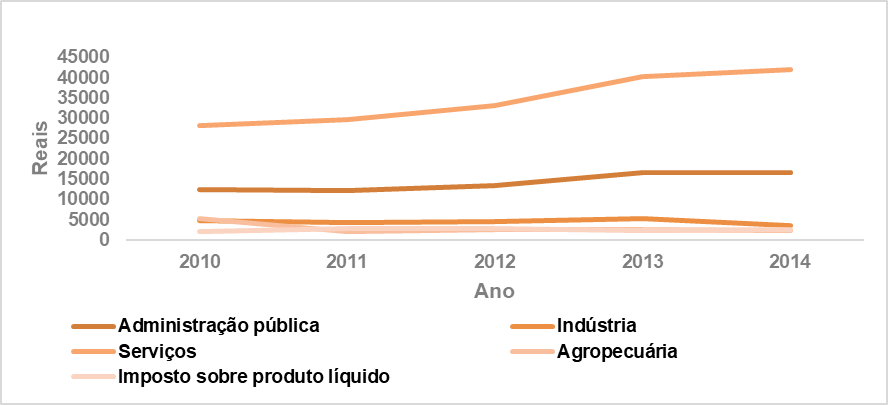
\includegraphics[width=0.85\linewidth]{produtos/proddois/image048}
	\caption{Série histórica da participação de cada setor no PIB do município de Monteiro Lobato entre os anos de 2010 a 2014.}
	\legend{Fonte: IMP SEADE, 2017.}
	\label{fig:image048}
\end{figure}

Como modo de comparação, o PIB do município pode ser relativizado com o PIB do Estado em que está contido. Dessa forma, Monteiro Lobato contempla, na média dos cinco anos apresentados, 0,0028382\% do PIB do Estado de São Paulo; 

\subsection{Disponibilidade de recursos}

A Lei Nº 1.657, de 27 de novembro de 2017, dispõe sobre o Plano Plurianual (PPA) do Município de Monteiro Lobato para o quadriênio de 2018/2021. De acordo com o Artigo 2º do PPA, os programas, diretrizes e metas integrantes constituem elo básico de integração e compatibilidade com o planejamento das prioridades a serem estabelecidas nas Leis das Diretrizes Orçamentárias (LDO) e as programações estabelecidas nos Orçamentos Anuais referentes aos exercícios financeiros de 2018 a 2021.

As estimativas de receitas e despesas para 2018 foram fixadas, através da Lei Nº 1.657, de 27 de novembro de 2017, de modo a conferir consistência ao PPA. O Orçamento do Município de Monteiro Lobato para o exercício financeiro de 2018 estima a Receita em R\$ 16.400.000,00, mediante a arrecadação dos Tributos, Rendas, Suprimentos e Outras Receitas Correntes e de Capital. Suas proporções e valores estão disponibilizados na \autoref{tab:receitas}. 

% Table generated by Excel2LaTeX from sheet 'receitas'
\begin{table}[htbp]
	\centering
	\caption{Receitas correntes em Monteiro Lobato.}
	\begin{tabular}{c|r}
		\rowcolor[rgb]{ .984,  .831,  .706} Impostos, Taxas e Contr. Mel. & 944.300,00 \\
		\rowcolor[rgb]{ .992,  .914,  .851} Receita de Contribuições & 73.000,00 \\
		\rowcolor[rgb]{ .984,  .831,  .706} Receita Patrimonial & 106.500,00 \\
		\rowcolor[rgb]{ .992,  .914,  .851} Transferências Correntes & 17.622.020,00 \\
		\rowcolor[rgb]{ .984,  .831,  .706} Outras Receitas Correntes & 22.380,00 \\
		\rowcolor[rgb]{ .992,  .914,  .851} \textbf{RECEITAS CORRENTES} & 18.768.200,00 \\
		\rowcolor[rgb]{ .984,  .831,  .706} Dedução para o FUNDEB & 2.368.200,00 \\
		\rowcolor[rgb]{ .992,  .914,  .851} \textbf{RECEITA FINAL} & 16.400.000,00 \\
	\end{tabular}%
	\label{tab:receitas}%
\end{table}%


A Despesa integrante para gestão do Município tem o mesmo valor da Receita de R\$ 16.400.000,00, e é desdobrada para a Câmara Municipal e para a Prefeitura Municipal nos valores de 765.000,00 e 15.635.000,00, respectivamente. O valor total da Despesa pode também ser desdobrado em relação às funções dos setores do Município ou em relação às subfunções, suas respectivas distribuições do valor de R\$ 16.400.00,00 são mostradas na \autoref{tab:despesas_funcoes} e \autoref{tab:despesas_subfunc}.

% Table generated by Excel2LaTeX from sheet 'despesas_funcoes'
\begin{table}[htbp]
	\centering
	\caption{Despesas por funções em Monteiro Lobato (ANO).}
	\begin{tabular}{c|r}
		\rowcolor[rgb]{ .984,  .831,  .706} Legislativa & 765.000,00 \\
		\rowcolor[rgb]{ .992,  .914,  .851} Administração & 1.600.950,00 \\
		\rowcolor[rgb]{ .984,  .831,  .706} Assistência Social & 678.550,00 \\
		\rowcolor[rgb]{ .992,  .914,  .851} Previdência Social & 610.000,00 \\
		\rowcolor[rgb]{ .984,  .831,  .706} Saúde & 3.924.600,00 \\
		\rowcolor[rgb]{ .992,  .914,  .851} Educação & 5.560.200,00 \\
		\rowcolor[rgb]{ .984,  .831,  .706} Cultura & 222.500,00 \\
		\rowcolor[rgb]{ .992,  .914,  .851} Urbanismo & 766.000,00 \\
		\rowcolor[rgb]{ .984,  .831,  .706} Gestão Ambiental & 115.000,00 \\
		\rowcolor[rgb]{ .992,  .914,  .851} Agricultura & 72.200,00 \\
		\rowcolor[rgb]{ .984,  .831,  .706} Comércio e Serviços & 112.800,00 \\
		\rowcolor[rgb]{ .992,  .914,  .851} Segurança Pública & 6.000,00 \\
		\rowcolor[rgb]{ .984,  .831,  .706} Transportes & 1.011.200,00 \\
		\rowcolor[rgb]{ .992,  .914,  .851} Desporto e Lazer & 200.000,00 \\
		\rowcolor[rgb]{ .984,  .831,  .706} Encargos Especiais & 255.000,00 \\
		\rowcolor[rgb]{ .992,  .914,  .851} Reserva de Contingência & 500.000,00 \\
		\rowcolor[rgb]{ .984,  .831,  .706} \textbf{TOTAL DA DESPESA} & 16.400.000,00 \\
	\end{tabular}%
	\label{tab:despesas_funcoes}%
\end{table}%

% Table generated by Excel2LaTeX from sheet 'despesas_subfunc'
\begin{table}[htbp]
	\centering
	\caption{Despesas por subfunções em Monteiro Lobato (ANO).}
	\begin{tabular}{c|r}
		\rowcolor[rgb]{ .984,  .831,  .706} \multicolumn{1}{c}{Ação Legislativa} & 765.000,00 \\
		\rowcolor[rgb]{ .992,  .914,  .851} \multicolumn{1}{c}{Administração Geral } & 1.600.950,00 \\
		\rowcolor[rgb]{ .984,  .831,  .706} \multicolumn{1}{c}{Assistência ao Idoso} & 52.000,00 \\
		\rowcolor[rgb]{ .992,  .914,  .851} \multicolumn{1}{c}{Assistência à Criança e Adolescente } & 124.000,00 \\
		\rowcolor[rgb]{ .984,  .831,  .706} \multicolumn{1}{c}{Assistência Comunitária } & 502.550,00 \\
		\rowcolor[rgb]{ .992,  .914,  .851} \multicolumn{1}{c}{Previdência Básica} & 610.000,00 \\
		\rowcolor[rgb]{ .984,  .831,  .706} \multicolumn{1}{c}{Atenção Básica} & 3.924.100,00 \\
		\rowcolor[rgb]{ .992,  .914,  .851} \multicolumn{1}{c}{Assistência Hospitalar e Ambulatorial} & 500.000,00 \\
		\rowcolor[rgb]{ .984,  .831,  .706} \multicolumn{1}{c}{Ensino Fundamental} & 3.558.700,00 \\
		\rowcolor[rgb]{ .992,  .914,  .851} \multicolumn{1}{c}{Ensino Médio } & 666.500,00 \\
		\rowcolor[rgb]{ .984,  .831,  .706} \multicolumn{1}{c}{Alimentação e Nutrição } & 290.000,00 \\
		\rowcolor[rgb]{ .992,  .914,  .851} \multicolumn{1}{c}{Educação Infantil} & 1.045.000,00 \\
		\rowcolor[rgb]{ .984,  .831,  .706} \multicolumn{1}{c}{Difusão Cultural } & 222.500,00 \\
		\rowcolor[rgb]{ .992,  .914,  .851} \multicolumn{1}{c}{Infraestrutura Urbana} & 10.000,00 \\
		\rowcolor[rgb]{ .984,  .831,  .706} \multicolumn{1}{c}{Serviços Urbanos} & 756.000,00 \\
		\rowcolor[rgb]{ .992,  .914,  .851} \multicolumn{1}{c}{Preservação e Conservação Ambiental } & 115.000,00 \\
		\rowcolor[rgb]{ .984,  .831,  .706} \multicolumn{1}{c}{Extensão Rural} & 72.200,00 \\
		\rowcolor[rgb]{ .992,  .914,  .851} \multicolumn{1}{c}{Turismo} & 112.800,00 \\
		\rowcolor[rgb]{ .984,  .831,  .706} \multicolumn{1}{c}{Defesa Civil} & 6.000,00 \\
		\rowcolor[rgb]{ .992,  .914,  .851} \multicolumn{1}{c}{Transporte Rodoviário} & 1.011.200,00 \\
		\rowcolor[rgb]{ .984,  .831,  .706} Desporto Comunitário & 200.000,00 \\
		\rowcolor[rgb]{ .992,  .914,  .851} Serviço da Dívida Interna & 10.000,00 \\
		\rowcolor[rgb]{ .984,  .831,  .706} Outros Encargos Especiais & 245.000,00 \\
		\rowcolor[rgb]{ .992,  .914,  .851} Reserva de Contingência & 500.000,00 \\
		\rowcolor[rgb]{ .984,  .831,  .706} \textbf{TOTAL DA DESPESA} & 16.400.000,00 \\
	\end{tabular}%
	\label{tab:despesas_subfunc}%
\end{table}%


\subsection{Indicadores sanitários, epidemiológicos, ambientais e socioeconômicos}
Os indicadores podem ser definidos como índices estatísticos que refletem uma determinada situação num dado momento. Podem ser empregados para avaliar políticas públicas, ou para comunicar ideias entre gestores e o público em geral, de forma direta e simples.
\subsubsection{Abastecimento de Água e Esgotamento Sanitário}
Este indicador é composto pela parcela da população com acesso adequado ao abastecimento de água e correta destinação e tratamento de esgoto sanitário. A \autoref{tab:indicadores_agua} mostra índices de atendimento total e urbano de água e esgoto para o município de Monteiro Lobato. Nota-se uma diferença bastante alta comparando-se os valores do município com a área urbana do mesmo.

% Table generated by Excel2LaTeX from sheet 'indicadores_agua'
\begin{center}
	\begin{table}[htbp]
	\centering
	\caption{Indicadores de Abastecimento de Água e Esgotamento Sanitário em Monteiro Lobato.}
	\begin{tabular}{P{25.93em}|c}
		\rowcolor[rgb]{ .969,  .588,  .275} 
		\multicolumn{1}{c}{\textcolor[rgb]{ 1,  1,  1}{\textbf{Indicadores }}} & \textcolor[rgb]{ 1,  1,  1}{\textbf{(\%)}} \\
		\rowcolor[rgb]{ .992,  .914,  .851} 
		\multicolumn{1}{c|}{Índice de atendimento total de água} & 49,57 \\
		\rowcolor[rgb]{ .984,  .831,  .706} 
		\multicolumn{1}{c|}{Índice de atendimento urbano de água} & 100 \\
		\rowcolor[rgb]{ .992,  .914,  .851} 
		\multicolumn{1}{c|}{Índice de coleta de esgoto} & 78,65 \\
		\rowcolor[rgb]{ .984,  .831,  .706} 
		\multicolumn{1}{c|}{Índice de tratamento de esgoto} & 100 \\
		\rowcolor[rgb]{ .992,  .914,  .851} Índice de atendimento total de esgoto referido aos municípios atendidos com água & 37,1 \\
		\rowcolor[rgb]{ .984,  .831,  .706} Índice de atendimento urbano de esgoto referido aos municípios atendidos com água & 85,97 \\
	\end{tabular}%
	\label{tab:indicadores_agua}%
\end{table}%
%Fonte: ~\cite{SNIS2016}.

\end{center}

\subsubsection{Resíduos sólidos}
A taxa de cobertura do serviço de coleta de resíduos sólidos domiciliares permite fornecer informações iniciais quanto ao manejo de resíduos no município, indicando a quantidade de resíduos que podem estar suscetíveis a disposição inadequada por falta de coleta. Tal fato pode acarretar proliferação de doenças, contaminação do solo ou corpo d’água e incômodo à população local pelo odor proveniente. Os indicadores do Sistema de Coleta encontram-se na \autoref{tab:indicadores_rs}.

% Table generated by Excel2LaTeX from sheet 'indicadores_rs'
\begin{table}[htbp]
	\centering
	\caption{Indicadores do Sistema de Coleta dos Resíduos Sólidos Domiciliares de Monteiro Lobato.}
	\begin{tabular}{P{6cm}|c}
		\rowcolor[rgb]{ .969,  .588,  .275} \multicolumn{2}{P{9cm}}{\textcolor[rgb]{ 1,  1,  1}{\textbf{Indicadores do Sistema de Coleta dos Resíduos Sólidos Domiciliares (RDO) (\%)}}} \\
		\rowcolor[rgb]{ .984,  .831,  .706} Taxa de cobertura do serviço de coleta de RDO em relação à população total do município & 71,48 \\
		\rowcolor[rgb]{ .992,  .914,  .851} Taxa de cobertura do serviço de coleta deRDO em relação à população urbana & 99,59 \\
	\end{tabular}%
	\label{tab:indicadores_rs}%
\end{table}%
%Fonte: ~\cite{SNIS2016}.


Informações mais completas a respeito do manejo de resíduos sólidos no município serão apresentadas no Produto 3 – Diagnóstico Municipal Participativo. 

\subsubsection{Doenças e endemias}

Sistema Único de Saúde (SUS) é a entidade que garante o acesso à saúde para qualquer cidadão brasileiro em última instância conforme previsto na Constituição Federal de 1988. Constituído por milhares de unidades hospitalares e ambulatoriais que tem por objetivo promover, prevenir e assistir à saúde, o SUS é a base fundamental para o diagnóstico referente ao acesso à saúde pública em qualquer território administrativo brasileiro. 

O município de Monteiro Lobato foi registrado em 2009 como detentor de dois estabelecimentos de Saúde do SUS. Em termos de profissionais da área, Monteiro Lobato conta com um coeficiente de 0,24 médicos registrados no CRM/SP para cada mil habitantes. Quanto a enfermeiros registrados no COREN/SP, Monteiro Lobato usufrui de 0,92 desses profissionais por mil habitantes. Na área de saúde bucal, Monteiro Lobato revela 0,92 dentistas para cada dois mil habitantes.

Com o objetivo de avaliar a eficácia do SUS, o Índice de Desempenho do SUS (IDSUS) surgiu em 2010 como ferramenta para verificar o cumprimento de seus princípios e diretrizes. Esse índice visa avaliar o SUS quanto à universalidade do acesso; integralidade, equidade, igualdade da atenção; descentralização com comando único; responsabilidade tripartite, regionalização e hierarquização da rede de serviços de saúde.

A \autoref{tab:desempenho} indica o desempenho das práticas mais imediatas referentes ao acesso à saúde pública básica do município de Monteiro Lobato, no ano de 2011, conforme os parâmetros mínimos definidos pelo IDSUS.

% Table generated by Excel2LaTeX from sheet 'desempenho'
\begin{table}[htbp]
	\centering
	\caption{Desempenho das práticas ao acesso à saúde pública básica.}
	\begin{tabular}{P{0.5\textwidth}|P{0.15\textwidth}}
		\rowcolor[rgb]{ .969,  .588,  .275} 
		\multicolumn{1}{c}{\textcolor[rgb]{ 1,  1,  1}{\textbf{Aspecto}}} & \textcolor[rgb]{ 1,  1,  1}{\textbf{Desempenho}} \\
		\rowcolor[rgb]{ .992,  .914,  .851} Cobertura populacional estimada pelas Equipes Básicas de Saúde & 115,20\% \\
		\rowcolor[rgb]{ .984,  .831,  .706} Cobertura populacional estimada pelas Equipes Básicas de Saúde Bucal & 97,00\% \\
		\rowcolor[rgb]{ .992,  .914,  .851} Cobertura populacional estimada pelas Equipes Básicas de Saúde Bucal & 100,00\% \\
	\end{tabular}%
	\label{tab:desempenho}%
\end{table}%

Também é possível avaliar questões ligadas à saúde por meio do índice FIRJAN de Desenvolvimento Municipal (IFDM), que avalia o desenvolvimento humano, econômico e social dos municípios anualmente e processa em coeficientes numéricos de 0 a 1. Sua base de cálculo é exclusivamente estatística, e se distingue do IDH porque esse tem um intervalo maior de coleta de dados. 		

Na área de saúde, o município de Monteiro Lobato recebeu na edição de 2015 (com ano base 2013), 0,8142, obtendo a classificação de alto desenvolvimento, que abrange o intervalo de 0,8 a 1,0. Essa avaliação coloca Monteiro Lobato como o 1784º lugar no ranking nacional na área de saúde, e o 345º lugar no Estado de São Paulo.

\subsubsection{Renda, pobreza e desigualdade}

O Índice de Desenvolvimento Humano (IDH) é um indicador que leva em conta três esferas: a educação, saúde e renda, ao contrário do PIB que considera apenas o desenvolvimento econômico e é uma proposta para uma visão mais holística para avaliar o desenvolvimento humano \cite{PNUD2017} O Índice de Desenvolvimento Humano Municipal (IDH-M) é o IDH para um município e é uma composição do IDHM Longevidade, que considera a esperança (ou expectativa média em anos) de vida ao nascer, do IDHM Educação, que leva em conta indicadores de escolaridade da parcela adulta da população bem como fluxo escolar da parcela jovem e do IDHM Renda, que considera a renda mensal per capita 

O gráfico da \autoref{fig:image049} demonstra o IDHM do município para os anos de 1991, 2000 e 2010 que correspondem aos anos de realização do Censo Demográfico.
 
  \begin{figure}[h!]
 	\centering
 	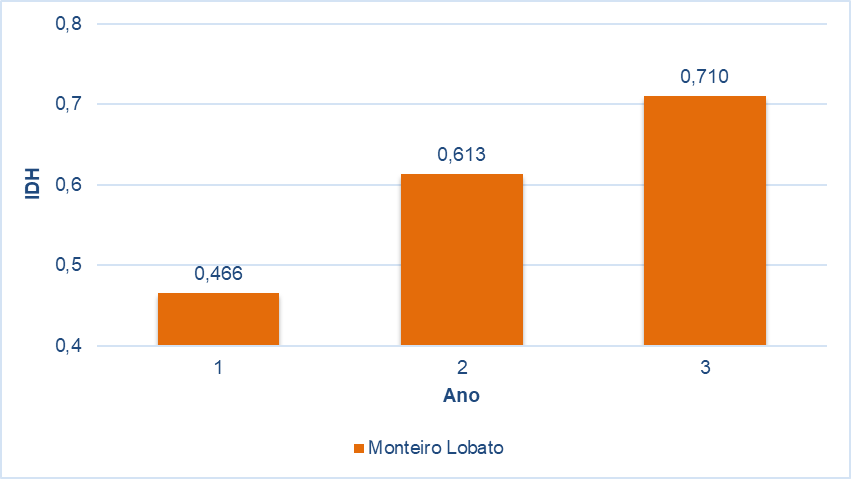
\includegraphics[width=0.8\linewidth]{produtos/proddois/image049}
 	\caption{Índice de Desenvolvimento Humano Municipal.}
 	\legend{Fonte: IMP SEADE, 2017.}
 	\label{fig:image049}
 \end{figure}


Analisando o gráfico é possível ver que para os períodos em questão o valor de índice cresceu numa taxa média de 19\% entre cada ano. Tal crescimento possibilitou uma transição de classificação para o município, saindo da classificação “muito baixa” no ano 1, para “alta” no ano 3, conforme pode ser observado na  \autoref{tab:valores_idh}.

% Table generated by Excel2LaTeX from sheet 'valores_idh'
\begin{center}
	\begin{table}[htbp]
	\centering
	\caption{Classificação para as faixas de valores de IDH.}
	\begin{tabular}{c|c}
		\rowcolor[rgb]{ .969,  .588,  .275} \multicolumn{1}{c}{\textcolor[rgb]{ 1,  1,  1}{\textbf{Faixas}}} & \textcolor[rgb]{ 1,  1,  1}{\textbf{Valores}} \\
		\rowcolor[rgb]{ .992,  .914,  .851} Muito Alto & De 0,800 a 1,000 \\
		\rowcolor[rgb]{ .984,  .831,  .706} Alto  & De 0,700 a 0,799 \\
		\rowcolor[rgb]{ .992,  .914,  .851} Médio & De 0,600 a 0,699 \\
		\rowcolor[rgb]{ .984,  .831,  .706} Baixo & De 0,500 a 0,599 \\
		\rowcolor[rgb]{ .992,  .914,  .851} Muito Baixo & De 0,000 a 0,499 \\
	\end{tabular}%
	\label{tab:valores_idh}%
\end{table}%
%Fonte: ~\cite{SEADE2017}.
\end{center}

Apesar do crescimento do IHD, Monteiro Lobato regrediu no ranking paulista ao longo dos anos avaliados. A \autoref{tab:idhm} mostra a posição segundo Ranking do estado de São Paulo para o município nos anos de 1991, 2000 e 2010.
 
% Table generated by Excel2LaTeX from sheet 'idhm'
\begin{table}[htbp]
	\centering
	\caption{Ranking de IDHM do estado de São Paulo - Posição de Monteiro Lobato.}
	\begin{tabular}{P{1,5cm}|P{1,5cm}|P{1,5cm}}
		\rowcolor[rgb]{ .969,  .588,  .275} 
		\multicolumn{3}{c}{\textcolor[rgb]{ 1,  1,  1}{\textbf{Ano}}} \\
		\rowcolor[rgb]{ .984,  .831,  .706} 1991  & 2000  & 2010 \\
		\rowcolor[rgb]{ .992,  .914,  .851} 457   & 488   & 534 \\
	\end{tabular}%
	\label{tab:idhm}%
\end{table}%


		\thispagestyle{headfootimage}
	\section*{Introdução}
	
	Este capítulo consiste no levantamento e análise do manejo dos resíduos sólidos gerados no município de Monteiro Lobato considerando a caracterização dos resíduos segundo a origem, o volume, as formas de destinação, a disposição final adotada e os respectivos custos associados. Além disso, descreve o acondicionamento, a coleta, o transporte e o transbordo, este quando aplicável, dos seguintes tipos de resíduos:
	
	\begin{itemize}
		\item [primeiro item] Resíduos Domiciliares;
		\item Resíduos de Limpeza Urbana;
		\item Resíduos de Estabelecimentos Comerciais e Prestadores de Serviços;
		\item Resíduos dos Serviços Públicos de Saneamento;
		\item Resíduos Industriais;
		\item Resíduos de Serviços de Saúde;
		\item Resíduos da Construção Civil;
		\item Resíduos Agrossilvipastoris;
		\item Resíduos de Serviços de Transportes; 
		\item Resíduos de Mineração; e
		\item Resíduos de Logística Reversa.
	\end{itemize}
	
	Para a elaboração deste diagnóstico, foi realizada uma reunião preliminar com a \gls{smaa}, \gls{ssm} e vice-prefeito para apresentação do objetivo da elaboração do \gls{pmgirs} de Monteiro Lobato e para compreender as responsabilidades e competências de cada secretaria. Após a reunião, foram encaminhados questionário dirigidos em forma de ofícios para as secretarias com questionamentos detalhados sobre a forma de gestão e gerenciamento dos resíduos sólidos gerados no município. As secretarias realizaram reuniões conjuntas para responder os ofícios e retornaram as respostas por meio eletrônico.
	
	A fim de complementar as informações secundárias apresentadas, foram realizadas visitas de campo acompanhadas pela \gls{smaa} para registros fotográficos do gerenciamento dos resíduos, realização de questionários estruturados para ampliar a participação dos munícipes na elaboração do \gls{pmgirs} e acompanhamento dos serviços de coleta dos resíduos comum e reciclável para determinação da rota.
	
	Os trajetos da coleta e destinação final dos resíduos foram determinados por coordenadas geográficas através do \gls{gps}, modelo Garmin etrex. Esses pontos foram inseridos no software ArcGIS e sobrepostos ao mapa da região.
	
	O questionário estruturado foi aplicado aos estabelecimentos comerciais responsáveis pela geração de óleos lubrificantes e pneus cujos endereços foram disponibilizados pela Prefeitura. O questionário foi realizado para conhecimento da geração e destinação final destes resíduos que devem apresentar sistema de logística reversa de acordo com o artigo 33 da Lei nº 12.305, de 02 de agosto de 2010.
	
	O município de Monteiro Lobato não dispõe de recurso específico destinado para o gerenciamento dos resíduos sólidos e de limpeza urbana. Neste contexto, foi solicitado à \gls{ssm}, via ofício, os custos associados para todas atividades do manejo de resíduos sólidos e serviços de limpeza urbana em relação aos salários dos funcionários, manutenção de equipamentos, contratos com empresas terceirizadas e gastos com transporte.
	
	A \gls{ssm} repassou um documento em formato .pdf com a relação de funções e atividades de vinte e nove funcionário e a folha de ponto. A fim de estimar qual o custo dos funcionários para a prefeitura em cada atividade de manejo de resíduos sólidos e de serviços de limpeza urbana, o valor total do salário base foi somado aos descontos pagos pela prefeitura (imposto de renda, \acrshort{inss} e demais contribuições) e ao \acrshort{fgts} e este total foi dividido entre os vinte e nove funcionários.
	
	Dependendo do cargo, das atribuições e das horas extras realizadas, a prefeitura ainda arca com uma base variável mensal em relação aos funcionários referente ao pagamento de horas extras e Salário-família. De acordo com a descrição da folha de pagamento disponibilizada, esta base variável é de aproximadamente R\$ 7.202,37 ao mês.
	
	Além disso, o município dispõe de cinco funcionários do Programa Frente de Trabalho, que qualifica profissionalmente e gera renda para cidadãos que se encontram desempregados e em situação de alta vulnerabilidade social, para colaboração em serviços de limpeza urbana, serviços de manutenção e serviços braçais. A estimativa do valor destinado a estes funcionários foi realizada considerando o salário base e o valor da cesta básica que o município disponibiliza para os funcionários.
	
	A partir do diagnóstico de resíduos sólidos é possível desenvolver um sistema de cálculo específico de custos dos serviços de limpeza urbana e de manejo de resíduos sólidos. A partir disso e da elaboração efetiva do \gls{pmgirs} de Monteiro Lobato, o município tem direito a ter acesso a recursos da União destinados para serviços relacionados a limpeza urbana e ao manejo de resíduos sólidos, de acordo com o artigo 18 da \gls{pnrs} (BRASIL, 2010a).
	
	O diagnóstico da situação de resíduos no município de Monteiro Lobato é indispensável para a definição de futuras diretrizes, identificação de gerenciamento inadequados, para o levantamento de ações mitigadoras e preventivas e para a elaboração de prognóstico (BRASIL, 2007a). Além disso, o levantamento do diagnóstico é de suma importância para a elaboração de propostas que visem a utilização racional de recursos ambientais, a redução de desperdícios, a minimização da geração de resíduos sólidos e o manejo ambientalmente adequado e economicamente viável.
	
	\section{Diagnóstico do sistema de limpeza urbana e manejo de resíduos sólidos}
	
	De forma resumida, o artigo 13 da Lei nº 12.305, de 02 de agosto de 2010 classifica os resíduos sólidos como:
	
	\begin{description}
		\item[\gls{rd}] originários de atividades domésticas em residências urbanas;
		\item[\gls{rlu}] originários da varrição, limpeza de logradouros e vias públicas e outros serviços de limpeza urbana;
		\item[\gls{rsu}] englobados nos resíduos domiciliares e nos resíduos de limpeza urbana;
		\item[\gls{rc}] gerados nessas atividades, exceto os serviços de limpeza urbana, de saneamento básico, de saúde, de construção civil e de transportes;
		\item[\gls{rspsb}] gerados nessas atividades, exceto os resíduos sólidos urbanos;
		\item[\gls{ri}] gerados nos processos produtivos e instalações industriais;
		\item[\gls{rss}] gerados nos serviços de saúde, conforme definido em regulamento ou em normas estabelecidas pelos órgãos do \gls{sisnama} e do \gls{snvs};
		\item[\gls{rcc}] gerados nas construções, reformas, reparos e demolições de obras de construção civil, incluídos os resultantes da preparação e escavação de terrenos para obras civis;
		\item[\gls{ra}] gerados nas atividades agropecuárias e silviculturais, incluídos os relacionados a insumos utilizados nessas atividades;
		\item[\gls{rst}] originários de portos, aeroportos, terminais alfandegários, rodoviários e ferroviários e passagens de fronteira;
		\item[\gls{rm}] gerados na atividade de pesquisa, extração ou beneficiamento de minérios;
		\item[\gls{rlr}] gerados após o uso pelo consumidor dos materiais provindos de fabricantes, importadores, distribuidores e comerciantes de agrotóxicos e suas embalagens, pilhas e baterias, óleos lubrificantes e suas embalagens, lâmpadas fluorescentes de vapor de sódio e mercúrio e de luz mista, produtos eletroeletrônicos e seus componentes.
		
	\end{description}
	
	\subsection{Resíduos Sólidos Urbanos}
	Os \gls{rsu} compreendem os resíduos domiciliares e os resíduos de limpeza urbana. Os resíduos domiciliares são os resíduos originários de atividades domésticas em residências urbanas. Os resíduos de limpeza urbana englobam os resíduos originários de varrição, de limpeza de logradouros, de vias públicas e de capina e poda (BRASIL, 2010a; BRASIL, 2007a).
	
	Além disso, nos casos em que os resíduos de estabelecimentos comerciais e prestadores de serviços são caracterizados como não perigosos, o poder público pode classificá-los como resíduos equivalentes aos resíduos domiciliares (BRASIL, 2010a).
	
	A geração estimada pela \gls{abrelpe} de  no Brasil foi de 78,3 milhões de toneladas em 2016, considerando a soma das projeções de cada região do país. Já a geração per capita apresentou um valor de aproximadamente 1,04 kg por habitante por dia (\gls{abrelpe}, 2016).
	
	Em relação a cobertura de coleta, o \gls{ipea} publicou em 2012 uma relação da coleta direta e indireta em área urbana e rural de resíduos sólidos urbanos entre os anos de 2000 e 2008 (tabela 1).
	
	Analisando a tabela 1 é possível verificar que a distribuição da taxa de cobertura de coleta de \gls{rsu} não é uniforme entre as regiões do país. Apesar de a coleta em área rural ter duplicado de 2000 a 2008 em porcentagem, a cobertura é muito baixa, sendo apenas 32,7 \% no país (IPEA, 2012a).
	
	As regiões Sudeste e Sul apresentaram a maior cobertura em área rural no ano de 2008, porém esses valores representam apenas 50 \% dos domicílios. Já a cobertura na área urbana apresenta valores acima de 95 \% de abrangência para todas as regiões do país. No entanto, o índice de coleta total das regiões Norte, Nordeste e Centro-Oeste ainda possuem deficiência (IPEA, 2012a).
	
	Em 2016, de acordo com as estimativas da \gls{abrelpe}, o índice de cobertura de coleta de \gls{rsu} do país cresceu para 91 \% e os índices da região Norte, Nordeste, Centro-Oeste, Sudeste e Sul aumentaram para, respectivamente, 81 \%, 79 \%, 94 \%, 98 \% e 95 \% (\gls{abrelpe}, 2016). Comparando as estimativas de 2008 da tabela 1 com as de 2016, a abrangência de coleta de \gls{rsu} foi ampliada, porém, a distribuição ainda não é equivalente entre todas as regiões.
	
	Aterro sanitário: Técnica de disposição de resíduos sólidos urbanos no solo, sem causar danos à saúde pública e à sua segurança minimizando os	impactos ambientais, método este que utiliza os princípios de engenharia (impermeabilização do solo, cercamento, ausência de catadores, sistema de
	drenagem de gases, águas pluviais e lixiviado) para confinar os resíduos e rejeitos à menor área possível e reduzi-los ao menor volume permissível,
	cobrindo-o com uma camada de terra na conclusão de cada jornada de trabalho, ou a intervalos menores, se necessário (adaptado da NBR 8419:1992).
	Aterro controlado: Forma inadequada de disposição final de resíduos e rejeitos, no qual o único cuidado realizado é o recobrimento da massa
	de resíduos e rejeitos com terra.
	Lixão: Forma inadequada de disposição final de resíduos e rejeitos, que consiste na descarga do material no solo sem qualquer técnica ou
	medida de controle.
	Tratando-se de disposição final no Brasil referente aos resíduos sólidos domiciliares e/ou urbanos, a sua relação e diferentes formas são apresentadas na figura 1, com dados de tonelada por dia para o ano de 2008. A disposição final mais utilizada no Brasil, assim como pode ser observado na figura 1, ainda se trata dos aterros sanitários. 
	
	Estima-se que, em 2016, 58,4 \% de \gls{rsu} do montante total do país tenha sido destinado a aterros sanitários, enquanto que 24,2 \% foi disposto em aterro controlado e 17,4 \% em lixões (\gls{abrelpe}, 2016). Neste contexto, é possível aferir que não houve significativa evolução em relação a disposição ambientalmente adequada dos resíduos sólidos no país.
	
	\colorbox{red}{REVISION NEEDED}
	%Aqui tínhamos falado para colocar definição de: aterro sanitário, controlado e lixão
	
	Apesar do Brasil ter um grande número de municípios contemplados com a disposição final dos \gls{rsu} em aterros sanitários, isso representa 40,20 \% do total, ou seja, menos da metade dos municípios brasileiros possuem aterros considerados sanitários. Quando se fragmenta, na Figura S, essa distribuição por regiões, percebe-se que as regiões Norte e Nordeste possuem um maior número de locais com disposição final ambientalmente inadequadas. A região Centro-Oeste apresenta uma relação numericamente comparável entre as formas atualmente adotadas de disposição final. As regiões Sudeste e Sul têm as melhores condições quanto à disposição final dos \gls{rsu}, e possui lixões em 10 \% e 12 \% dos municípios, respectivamente.
	
	O serviço público é responsável pela gestão e gerenciamento dos serviços de limpeza urbana e pelo manejo dos resíduos domiciliares, de modo a atender ao plano municipal de gestão integrada de resíduos sólidos (BRASIL, 2010a).
	
	Se o poder público classificar os resíduos de estabelecimentos comerciais e prestadores de serviço como equivalentes à resíduos domiciliares, o gerenciamento será de responsabilidade do poder público. No entanto, se os resíduos de estabelecimentos comerciais e prestadores de serviço forem caracterizados como perigosos ou não forem equiparados à resíduos domiciliares por sua natureza, composição, volume ou quantidade superior a determinada pelo município, os geradores estarão sujeitos a elaborar o próprio plano de gerenciamento (BRASIL, 2010a).
	
	No município de Monteiro Lobato os \gls{rsu} são divididos em duas categorias: resíduos sólidos comuns e resíduos sólidos recicláveis. Os resíduos sólidos comuns no município consistem em resíduos considerados domiciliares (com exceção de recicláveis), rejeitos e matéria orgânica. 
	Os resíduos oriundos de serviços de limpeza urbana como varrição, desobstrução de sarjetas, poda e capina são usualmente considerados pelo município como resíduos comuns e recebem, em sua maioria, a mesma destinação e disposição final que os resíduos domiciliares e de estabelecimentos comerciais e prestadores de serviços.
	
	Os resíduos sólidos recicláveis são constituídos de materiais plásticos de diversas categorias (PET, PP, PEBD, PEAD entre outros), vidro, metal, papel e papelão, possuem valor agregado e devem voltar ao sistema produtivo como matéria prima para fabricação de novos produtos através da reciclagem e/ou reaproveitamento.
	
	\subsection{Resíduo Sólido Comum}
	
	Em relação à cobertura de coleta de \gls{rsu} do município de Monteiro Lobato, a tabela 2 apresenta a relação entre população (total, urbana e rural) atendida pelo serviço de coleta, dados disponibilizados entre 2009 e 2015 (SNIS, 2009 a 2015).
	
	Ao analisar a tabela 2, verifica-se a deficiência na declaração dos dados pelos municípios para o Sistema Nacional de Informações sobre Saneamento (SNIS). A ausência de dados consistentes ao longo da Série Histórica prejudica a interpretação e expõe uma fragilidade em relação a qualidade das informações.
	
	Considerando-se a fragilidade dos dados de cobertura de coleta, as discussões serão baseadas principalmente nas informações prestadas pela autoridade pública municipal de Monteiro Lobato.
	
	Os dados obtidos sobre os resíduos comuns foram coletados em três etapas. Primeiro foram encaminhados questionários dirigidos em forma de ofício para \gls{smaa} bem como para a \gls{ssm} e separados por origem de resíduos: \gls{rsu}, \gls{rss}, Resíduos de Construção Civil (RCC). Nesse questionário foi indagado sobre as condições de coleta, equipamentos utilizados, número de funcionários responsáveis pelas atividades, custo associado, destinação e disposição final dos resíduos.
	
	Em seguida, na segunda etapa através da ferramenta Excel 2016, foram realizadas avaliações estatísticas dos dados de disposição final destes resíduos no aterro sanitário de Tremembé administrado pela companhia ESTRE-Resicontrol, que forneceu uma série histórica entre 2 de janeiro de 2014 até 9 de outubro de 2017.
	
	Por fim, foram realizados registros fotográficos das formas de acondicionamento dos resíduos comum e dos equipamentos e materiais utilizados, a fim de validar as respostas dos questionários dirigidos.
	
	\subsubsection{Acondicionamento}
	
	De acordo a \gls{ssm}, o acondicionamento coletivo de resíduos comuns no município é composto por 59 lixeiras. Os resíduos comuns domiciliares e comerciais ficam normalmente armazenados em lixeira de ferro de, aproximadamente, 2 x 1 x 1 metros, como apresentado na parte superior da figura 2. Existem também as lixeiras de madeira, que apresentam dimensões de 2 x 1 x 1 m ou de 1,20 x 1 x 1 m (parte inferior da figura 2). Foi possível verificar que, apesar de as lixeiras apresentarem um volume significativo, alguns resíduos são dispostos inadequadamente no solo ao lado das lixeiras. 
	
	Os resíduos introduzidos nas lixeiras são embalados pelos munícipes em sacolas de supermercado, saco plástico pretos de volumes distintos, caixas de papelão entre outros materiais. Entretanto, muitos resíduos sólidos são dispostos nas lixeiras sem o devido acondicionamento, o que prejudica o processo de coleta por parte dos funcionários, como mostrado na Figura 3.
	
	As lixeiras maiores costumam compor as áreas comuns dos bairros, no entanto, alguns moradores possuem o próprio cesto de lixo, como exemplificado pela figura 6. Existe ainda o hábito de alguns moradores pendurarem sacos plásticos com os resíduos em ganchos no portão da residência, como apresentado na figura 7.
	
	\subsubsection{Coleta, transbordo e transporte}
	
	Os resíduos comuns coletados no município são compostos por resíduos sólidos produzidos por estabelecimentos comerciais e prestadores de serviço, residências de área urbana e área rural, resíduos de caráter domiciliar não reciclável de estabelecimentos particulares geradores de \gls{rss}, Resíduos de Serviços de Transporte (RST) e Resíduos Industriais (RI), além de parte dos resíduos oriundos da limpeza pública. Essa abrangência na coleta ocorre devido à inexistência de regulamentação pelo município quanto ao tipo de gerador e suas obrigações legais conforme preconiza a \gls{pnrs} (Lei nº 12.305 de 2010).
	
	A coleta municipal dos resíduos sólidos comuns ocorre às segundas, terças, quintas e sextas-feiras, de acordo com os horários apresentados na tabela 3.  O município dispõe de um caminhão do tipo compactador de 19 m$^{3}$ (vide figura 8) com o qual é realizada a coleta.
	
	Das 59 lixeiras coletivas existentes no município e conforme descrição da \gls{ssm}, o caminhão coletor passa pelos seguintes bairros com respectivos números de lixeiras coletivas após sair da \gls{ssm}:
	
	\begin{itemize}
		\item SP 50 Bairro Taquari – 4 lixeiras; 
		Bairro Descoberto – 1 lixeira; 
		Bairro Ponte Nova – 3 lixeiras; 
		Estrada do Livro – 2 lixeiras; 
		Bairro Pedra Branca – 5 lixeiras; 
		Estrada São Francisco – 6 lixeiras; 
		Centro – 12 lixeiras; 
		Bairro Alpes do Boquira – 1- lixeira; 
		SP 50 Bairro São Benedito – 13 lixeiras; 
		Estrada Ito Rennó – 2 lixeiras; 
		Estrada Cruzeiro – 1 lixeira; 
		Bairro do Souzas – 4 lixeiras; 
		Estrada Fabiano – 2 lixeiras; 
		Estrada Pandavas – 3 lixeiras.
	\end{itemize}

	Durante o percurso realizado em uma segunda-feira foram obtidas as coordenadas geográficas das lixeiras cujo resíduo sólido comum foi recolhido através do GPS. A rota dessa coleta passou por 37 lixeiras cujas localizações são apresentadas na figura 10. 
	
	A coleta dos pontos geográficos das lixeiras ocorreu juntamente com o registro fotográfico de cada local.  Durante o percurso, notou-se que em alguns pontos há o descarte, em local inadequado, do líquido acumulado no caminhão compactador, conforme ilustra a figura 9.
	
	Para a retirada dos resíduos das lixeiras é feita uma manobra com o caminhão, em que o mesmo se aproxima de ré até ficar bastante próximo da lixeira, como ilustram as figuras 11 e 12. A figura 12 também mostra a disposição inadequada dos resíduos sólidos no solo, fora da lixeira.
	
	Em dezembro de 2017, o percurso do caminhão coletor foi acompanhado durante alguns dias da semana e sua rota registrada através do GPS. A obtenção dessas rotas colabora com o possível traçado de caminhos mais otimizados, e assim, o município teria um transporte mais rápido e com menor consumo de combustível, gerando menor custo e menor emissão de gases de efeito estufa.
	
	Para os dias de coleta de resíduo comum (segunda, terça, quinta e sexta-feira), não há uma rota pré-definida pela secretaria, ficando a critério do motorista responsável contanto que atenda a todos os locais em que a coleta deve ser realizada. A figura 13 apresenta o percurso realizado referente à uma quinta-feira.
	
	De acordo com informações da \gls{ssm}, a partir de 2019, após finalizada a coleta dos resíduos comuns às 16 horas (às segundas, terças, quintas e sextas-feiras,), o caminhão segue em direção ao aterro sanitário de Tremembé para a devida disposição final. O percurso realizado até o aterro sanitário é de aproximadamente 48 km (figura 16).
	
	Nesses dias em que o resíduo é encaminhado ao aterro sanitário, a média diária que o caminhão percorre é de 207,7 km para realização da coleta, transporte e retorno à base. Para execução da coleta o município dispõe de três funcionários, sendo um motorista e dois coletores.
	
	\subsubsection{Disposição final}
	
	O aterro sanitário de Tremembé pode receber resíduos Classe I, II A e II B. Ao chegar, o caminhão passa por uma balança rodoviária para aferição de sua massa e posteriormente o resíduo é encaminhado para o local de despejo onde é finalmente disposto em local adequado. Em seguida, o caminhão retorna à balança para aferir novamente sua massa.
	De uma forma geral, o sistema de coleta de resíduos comuns pode ser esquematizado conforme a figura 17.
	
	\subsubsection{Volume}
	
	Através da avaliação da série histórica dos dados cedidos pelo aterro sanitário de Tremembé, foi possível aferir algumas características existentes no município e sua dinâmica. O conhecimento desses dados é importante para entender o comportamento de geração de resíduos sólidos comuns, e assim elaborar ações e metas que auxiliem na melhoria da gestão dos resíduos.
	
	Nessa avaliação procurou-se conhecer a variação de geração do resíduo ao longo dos meses, onde foi possível perceber que, entre os anos avaliados, ocorreu uma tendência de maior geração entre os meses de dezembro e março, sendo janeiro o mês mais expressivo ao longo dos anos. Uma hipótese para explicar esse fato seria o acréscimo do número de turistas na região, no período.
	
	Há também um período de menor geração que ocorre entre agosto e setembro, conforme Figura 18. No apêndice A consta a geração pontual que cada segunda, quarta e sexta feira produzia ao longo dos meses comparativamente com as médias anuais e diárias ao longo dos anos avaliados (2014-2017).
	
	Nesta avaliação também foi possível obter e compreender como é a dinâmica de produção do resíduo comum pelos munícipes. Neste caso percebe-se que os dias que acontecem as coletas de maiores quantidades são segundas-feiras como pode ser vislumbrado na figura 19.
	
	Essa maior quantidade coletada às segundas possivelmente é em decorrência dos finais de semana, quando os munícipes ficam mais tempo em suas casas e também ocorre aumento do número de turistas na região. A geração de resíduos ao longo da semana tem uma dinâmica em que a produção em dias úteis é mais expressiva que a produção de resíduos nos finais de semana.
	
	A cada dia de coleta dos \gls{rsu} comuns recolhem-se resíduos acumulados durante 2 a 3 dias pela população em Monteiro Lobato, como mostra a Tabela C.
	
	Outro ponto a ser destacado é a ocorrência da geração per capita diária de resíduos pelos munícipes e como ela se comporta ao longo dos anos observados. Para essa avaliação foram utilizadas as estimativas populacionais fornecidas pelo Instituto Brasileiro de Geografia Estatística (IBGE), bem como o total anual gerado. Nota-se que de 2015 até 2017, a geração per capta regride, como pode ser visto na figura 21.
	
	Analisando os dados foi possível verificar que a contribuição média diária para a geração de resíduos comuns é de 0,48 kg por habitante, totalizando em uma geração média de 4,44 toneladas por coleta e uma produção média mensal de 65,31 toneladas (2014-2017).
	
	\subsubsection{Caracterização gravimétrica} 	
	A caracterização gravimétrica tem como premissa entender a composição de todo o resíduo gerado em uma amostra, dividindo-o em categorias. Com este intuito, caracterizou-se o \gls{rsu} comum no mês de dezembro de 2017.
	
	Para isso, foram utilizados uma balança com contrapeso e capacidade para 180 kg (+/-) 2 kg e um dinamômetro com capacidade para 50 kg (+/-) 0,050 kg para os resíduos mais leves (figura 22).
	
	Para a caracterização dos \gls{rsu}, usou-se de forma adaptada para as características locais, a Norma NBR 10004/2004 na classificação e separação por tipo dos resíduos triados, a Norma NBR 1007/2004 na amostragem, e o Manual de Gestão dos Resíduos Sólidos do Instituto Brasileiro de Administração Municipal (IBAM, 2001) para o procedimento de gravimetria.
	
	No processo de caracterização gravimétrica foi observado que o caminhão compactador atualmente destinado ao recolhimento dos resíduos no município coleta aproximadamente 2/3 do que é gerado nas segundas e quartas-feiras, sendo, assim, necessária a complementação da coleta com outro caminhão. Este caminhão tem como função executar somente a coleta seletiva, no entanto, devido a problemas por falta de manutenção na frota, ambas as coletas são feitas pelo mesmo veículo.
	
	\paragraph{\textbf{Metodologia da caracterização gravimétrica:}}
	
	A caracterização dos resíduos da coleta comum foi realizada entre os dias 11 e 16 de dezembro de 2017. Em cada avaliação era utilizado material proveniente da coleta do dia anterior. Após a retirada das lixeiras públicas, o resíduo era transportado para um pátio da \gls{ssm} onde ficava armazenado. O pátio possuía impermeabilização de cimento, porém não havia cobertura. No período da caracterização não houve incidência de chuva.
	
	Foram realizadas 3 amostragens, uma para cada dia de coleta semanal (antigamente realizada às segundas, quartas e sextas-feira). No dia seguinte a coleta, os resíduos armazenados eram espalhados pelo pátio, homogeneizados, quarteados e metade da amostra era removida com auxílio de uma escavadeira. O mesmo processo era aplicado na porção restante. Após, de forma manual, os sacos contendo resíduos eram abertos e o conteúdo novamente espalhado pelo pátio, homogeneizado e, posteriormente espalhados aleatoriamente de forma circular para retirada de 1 m$^{3}$ de resíduos.
	
	Para a pesagem dos resíduos foi utilizado um tambor cilíndrico de plástico de 0,2 m$^{3}$. O preenchimento do tambor foi feito recolhendo resíduos de 5 pontos distintos, percorrendo a circunferência. Sequencialmente, despejou-se novamente o conteúdo do tambor no chão e procedeu-se com a separação dos materiais por tipos e repesagem de cada tipo conforme pode ser observado na figura 24.
	
	Devido ao baixo efetivo e à impossibilidade de aferição de resíduos com menor massa, a divisão por tipos de \gls{rsu} se limitou de acordo com a Tabela S.
	
	
	\paragraph{\textbf{Resultados da caracterização gravimétrica:}}
	
	Com os dados de cada amostra foi possível obter uma média da composição gravimétrica da coleta comum realizada no município, segundo a tabela 4. No final de semana antecedente à caracterização gravimétrica, houve uma forte chuva no município, e como os resíduos ficam dispostos nas lixeiras coletivas para posterior coleta, a composição gravimétrica da coleta de segunda-feira pode ter sofrido variação na massa em decorrência do volume de água envolvido juntamente aos resíduos.
		
	Foram obtidas as densidades aparente dos resíduos e sua média referentes aos dias de avaliação, como pode ser observado na tabela 5. A densidade média é um valor que pode ser utilizado para o dimensionamento de equipamentos de transporte, instalações de transbordo e tratamento de resíduos sólidos (MONTEIRO, 2001).
	
	A média de geração dos \gls{rsu} comuns referente aos dias de pico avaliados encontra-se ilustrada na Figura 25. O resultado caracteriza-se pelo maior conteúdo de material orgânico, atingindo 34,1 \% do total do \gls{rsu}. Em seguida, com 13 \% e 12,8 \% respectivamente, ocorre a geração de materiais higiênicos e tecidos, sendo em sua maioria roupas ainda em bom estado (figura 26). 
	
	Os plásticos como um todo somam 18 \% do \gls{rsu} gerado, sendo 11,4 \% de plástico fino e 6,6 \% de plástico duro; 9,9 \% do total do \gls{rsu} são constituídos de papel e papelão; 5,0 \% são constituídos de metais ferrosos, não ferroso e alumínio; 2,7 \% por madeiras tratadas e não tratadas (naturais); 1,7 \% por pneus; 1,4 \% por vidros coloridos e transparentes; e 1,4 \% por outros materiais que são passíveis de logística reversa e  materiais de \gls{rss} que devem ser acondicionados e armazenados diferenciadamente para posterior tratamento (seringas, medicamentos e embalagens medicamentosas).
	
	Para obtenção de um resultado mais próximo da realidade do município, faz-se necessária outra caracterização em um período de baixa geração ou menor sazonalidade.
	
	\subsubsection{Custos}
	
	A equipe responsável pelos serviços de coleta de resíduos sólidos comuns é composta por três funcionários, sendo dois coletores e um motorista. De acordo com documento fornecido pela \gls{ssm} em 2017, considerando os custos de salário base, descontos e FGTS, estima-se que sejam destinados de remuneração, R$ 1.841,08 para cada funcionário. Assim, o valor total é de R$ 5.523,24 para os três funcionários.
	
	Em relação ao custo destinado à manutenção de equipamentos para o serviço de coleta, em 2017, a \gls{ssm} declarou ser gasto uma média de R\$ 1.800,00 em manutenção de equipamentos do serviço de coleta comum.
	
	Em relação ao transporte da coleta comum, a estimativa do gasto foi calculada considerando a média da quilometragem da rota percorrida para coleta, transporte e disposição final até o aterro sanitário às segundas, terças, quintas e sextas-feiras (207,7 km por dia). 
	
	Considerando o preço do litro do diesel disponibilizado pela \gls{ssm} de Monteiro Lobato (XXX) e a quilometragem total rodada para os quatro dias (830,8 km), o gasto referente ao transporte do serviço de coleta comum é de, aproximadamente, R\$ 3.509,11. A tabela 6 apresenta o resumo dos custos associados ao serviço público de coleta de resíduo comum de Monteiro Lobato.
	
	O custo associado ao serviço de disposição final do resíduo comum de Monteiro Lobato realizado no aterro sanitário ESTRE-Resicontrol foi obtido através da solicitação dos contratos desde a validação do primeiro contrato com a Secretaria de Finanças do município. A tabela 7 apresenta o histórico de custo associado ao serviço de disposição final do resíduo comum coletado pelo município do período de 2014 a 2017, considerando que são realizados contratos anuais com a ESTRE-Resicontrol.
	
	\subsection{Resíduos da Coleta Seletiva}
	
	Através da obtenção dos dados referentes a geração e coleta de resíduos sólidos recicláveis da plataforma Série Histórica do SNIS para o ano de 2015, a tabela 8 foi construída (SNIS, 2009 a 2015). Analisando a tabela, observa-se que a taxa de cobertura de coleta seletiva porta-a-porta do país abrange apenas metade da população urbana e que este valor não é homogêneo para cada região.
	
	Enquanto a região Sul possui a maior taxa de coleta seletiva, abrangendo 77 \% da população urbana, as regiões Norte e Nordeste apresentam taxa de coleta seletiva em torno de apenas 15 \%. As regiões Centro-Oeste e Sudeste são as que mais se assemelham a taxa de cobertura do país.
	
	A região Sul se destaca em relação aos outros parâmetros analisados de taxa de material recolhido em relação ao total de resíduos sólidos domésticos (exceto matéria orgânica e rejeitos), massa per capita de materiais recicláveis coletados e massa recuperada em relação a população urbana.
	
	Os valores da tabela 8 indicam que, em geral, o Brasil ainda conta com um sistema precário de coleta seletiva e recuperação dos materiais recolhidos. Para melhorar esse panorama, a taxa de cobertura de coleta seletiva deveria ser mais abrangente e, para que o sistema fosse efetivo, seria necessário maior investimento em educação ambiental para que a população fosse mobilizada e sensibilizada a fazer a correta segregação do resíduo domiciliar. Através dessas ações, a taxa de \gls{rsu} destinada a aterros sanitários pode diminuir consideravelmente.
	
	Os dados primários sobre os resíduos recicláveis em Monteiro Lobato foram obtidos por meio de questionário dirigido às \gls{smaa} e \gls{ssm} e avaliação presencial da coleta municipal.
	
	\subsubsection{Acondicionamento}
	
	Os resíduos recicláveis são acondicionados de forma semelhante à dos resíduos sólidos comuns, em sacos plásticos ou em sacolas de supermercados. Da mesma forma, o armazenamento destes resíduos é semelhante ao dos resíduos sólidos comuns, sendo pendurados em portões ou dispostos nas lixeiras de ferro ou de madeira.
	
	Além disso, resíduos maiores como caixas de papelão e isopor costumam ser acondicionados sem nenhuma forma de revestimento nas lixeiras, como apresentado na figura 27.
	
	\subsubsection{Coleta, Transbordo e Transporte}
	
	Um problema pelo qual o município passa é em relação ao armazenamento e coleta dos resíduos recicláveis. Atualmente, a coleta do resíduo reciclável ocorre às quartas-feiras em período integral, das 7h às 16h.
	Como o município não dispõe de lixeiras específicas para resíduos comuns e resíduos recicláveis ou de estratégias para diferenciar o acondicionamento, os sacos plásticos de resíduos comuns e recicláveis ficam misturados nas lixeiras e os coletores não são capazes de diferenciar as composições dos sacos no momento da coleta. Deste modo, durante as coletas dos resíduos recicláveis são coletados apenas os resíduos de fácil identificação, como caixas de papelão e garrafas, como exemplificado na figura 28.
	
	O serviço de coleta de resíduos sólidos recicláveis é realizado pelos mesmos três funcionários responsáveis pela coleta de resíduos comuns. A coleta dos recicláveis ocorre através de um caminhão tipo compactador exclusivo com capacidade de 15 m$^{3}$(vide figura 29), que percorre todo o município e encaminha os resíduos para Jacareí.
		
	Conforme descrição da \gls{ssm}, a coleta de resíduos sólidos recicláveis passa pelas mesmas 59 lixeiras nas quais são armazenados os resíduos sólidos comuns, cujas localizações foram discutidas para o resíduo sólido comum.
	O processo de retirada dos resíduos recicláveis é o mesmo que o realizado para os resíduos sólidos comuns. É feita uma manobra com o caminhão aproximando-o de ré até próximo a lixeira como ilustra a figura 30. Nesta figura é possível visualizar a dificuldade dos coletores para coleta dos resíduos que não são adequadamente acondicionados.
	
	Como descrito anteriormente, na segunda semana de dezembro de 2017 os percursos de coleta foram acompanhados e as rotas foram registradas através do GPS. Nesse ano, a coleta seletiva costumava ocorrer às terças e quintas-feiras no período da tarde, ao invés de ser às quartas-feiras como ocorre atualmente. Na Figura 32, é apresentada a rota realizada para a coleta seletiva, referente a uma quinta-feira, mas que pode ser refletida a rota atualmente realizada.
	
	Ao término de toda a coleta, é feito um percurso até a \gls{urbam} em São José dos Campos, para que seja efetuada a triagem deste material nas instalações do aterro. De acordo com os dados disponibilizados pela \gls{ssm}, a quilometragem média percorrida para realização da coleta dos resíduos sólidos recicláveis no município e armazenamento na garagem da \gls{ssm} é de 20 km. No entanto, no terceiro dia de coleta de recicláveis, os resíduos acumulados são encaminhados à \gls{urbam} e o caminhão retorna à base, a uma distância média percorrida de 123,3 km, levando em consideração que a distância entre Monteiro Lobato e a \gls{urbam} é de aproximadamente 48 km. A localização da \gls{urbam} em relação ao município é apresentada na figura 33.
	
	\subsubsection{Disposição final}
	
	Como descrito anteriormente, na terceira coleta de resíduos sólidos recicláveis, o caminhão encaminha os resíduos acumulados até a Urbanizadora Municipal de São José dos Campos – \gls{urbam}.
	
	Quando o caminhão chega à \gls{urbam}, os resíduos são encaminhados à área de triagem. Após a deposição do material na área de triagem da \gls{urbam}, os resíduos passam por uma esteira rotativa sendo separados manualmente por catação, do início ao fim do processo. Os materiais selecionados e separadas são enfardados para então serem comercializado, enquanto os materiais descartados na triagem, serão destinados a área de aterramento onde receberão sua disposição final.
	
	De uma forma geral, o sistema de coleta de resíduos seletivos pode ser esquematizado conforme a figura 34.
	
	\subsubsection{Volume gerado}
	
	Através de dados disponibilizados pela \gls{ssm}, dos valores totais mensais e a quantidade de coletas realizadas dos meses de março a outubro de 2017, foi possível realizar algumas análises sobre a dinâmica e atuação do município para com os resíduos recicláveis. A avaliação dessas informações permite que sejam compreendidos a dinâmica de geração de resíduos recicláveis e os hábitos de segregação entre resíduos recicláveis e comuns e auxilia no desenvolvimento de diretrizes e ações que visem a melhoria do gerenciamento dos resíduos recicláveis.
	
	Com base nos dados fornecidos e projeções populacionais do IBGE foi possível estimar a geração per capita diária de resíduos sólidos recicláveis entre março e outubro de 2017 (vide figura 35). Percebe-se uma tendência entre os meses de março e agosto, que apresentam valor per capita diário de aproximadamente 0,04 kg por habitante por dia. Para os meses de setembro e outubro é observada uma queda brusca na geração.
	
	Com a estimativa desses dados é possível verificar que o potencial de reciclagem do município é muito baixo. Considerando que a geração per capita de resíduo sólido domiciliar de Monteiro Lobato é a soma entre a geração per capita diária de resíduo comum e a geração per capita diária de resíduo reciclável, a geração per capita de resíduo reciclável representa, aproximadamente, 8 \% da geração per capita total.
	Na coleta dos \gls{rsu} seletivos, recolhe-se todo o resíduo gerado pela população durante uma semana anterior. Um problema recorrente no município é a ausência de lixeiras separadas para resíduos recicláveis, o que pode acarretar em uma diferença na quantidade de resíduos recicláveis coletados para a quantidade real de resíduos colocados nas lixeiras além de haver dificuldade na diferenciação dos sacos de resíduos recicláveis dos comuns pelos coletores.
	
	\subsubsection{Caracterização gravimétrica}
	
	\paragraph{\textbf{Metodologia da caracterização gravimétrica}}
	
	A caracterização gravimétrica e a avaliação dos \gls{rsu} seletivos ocorreram igualmente ao processo descrito para a metodologia dos resíduos sólidos comuns (item 1.2.5). Para os resíduos provenientes da coleta seletiva foram realizadas 2 amostragens dos seus respectivos dias de coleta semanal (terça e quinta-feira, dias antigos de coleta reciclável referente à data em que essa caracterização foi realizada, em 2017). Devido ao baixo efetivo e à impossibilidade de aferição de resíduos com menor massa, a divisão por tipos de resíduos se limitou à disposta na tabela 3. Não houveram alterações nas condições climáticas que comprometessem a caracterização desses resíduos.
	
	\paragraph{\textbf{Resultados da caracterização gravimétrica}}
	
	Com os dados de cada amostra foi possível obter uma média da composição gravimétrica da coleta comum realizada no município, conforme a tabela 10.
	
	Medindo-se as amostras obteve-se as densidades aparentes dos resíduos da coleta seletiva referentes aos dias de avaliação, bem como a média como pode ser observado na tabela 11.
	
	A característica dos \gls{rsu} seletivos (figura 36) no período de maior geração no município é de 40,5 \% de papelão como material presente em maior quantidade seguido de plásticos totalizando 25,1 \% sendo que desses, 14,4 \% são plásticos duros e 10,7 \% são plásticos finos. Vidros coloridos e transparentes contribuem com 19,4 \% e papeis representam 3,8 \%, seguidos pelos materiais que são passíveis de logística reversa (embalagens de óleos automotivos, lâmpadas fluorescentes, equipamento eletroeletrônicos e pilhas) e materiais de \gls{rss} (seringas, medicamentos e embalagens medicamentosas), que devem ser acondicionados e armazenados diferenciadamente para posterior tratamento, constituindo estas classes 2,4 \% do total. 
	Na caracterização gravimétrica também foi catalogada a presença de materiais higiênicos (2,3 \%) e materiais orgânicos (2,1 \%), os quais contaminam materiais recicláveis, podendo reduzir ou até inviabilizar a reciclagem desses materiais com tal potencial. Em menor proporção ocorreram embalagens Tetra Pak com 1,3 \%, metais diversos 1,1 \%, isopor 0,5 \% e tecido 1,4 \% conforme demonstra a figura 36.
	
	Para um resultado mais próximo da realidade do município, faz-se necessária outra caracterização em um período de baixa geração ou menor sazonalidade.
	
	\subsubsection{Custos}
	
	A distribuição dos custos relacionados aos resíduos recicláveis é similar aos custos referentes aos resíduos comuns. Os funcionários responsáveis pelo serviço de coleta de resíduos recicláveis são os mesmos para a coleta de resíduo comum. Desta forma, o salário destinado aos três funcionários engloba o serviço de coleta de resíduos comum e reciclável.
	De acordo com dados fornecidos pela \gls{ssm}, o valor destinado à manutenção de equipamentos para este serviço é R\$ 1.800,00 por mês. 
	
	Em relação ao transporte, a estimativa do valor gasto foi a mesma que para a despesa relacionada ao resíduo sólido comum. O cálculo foi feito considerando a média da quilometragem da rota percorrida apenas para coleta dos resíduos (20 km) e a média da quilometragem da coleta, transporte e destinação final até a \gls{urbam}, quando realizada a terceira coleta de resíduos recicláveis (123,3 km).
	
	Considerando o preço do litro do diesel disponibilizado pela \gls{ssm} de Monteiro Lobato e a quilometragem total rodada, o gasto referente ao transporte do serviço de coleta reciclável é de, aproximadamente, R\$ 438,70. A tabela 12 apresenta o resumo dos custos associados ao serviço público de coleta de resíduo comum de Monteiro Lobato.

	Como o município não apresenta contrato firmado com a \gls{urbam} de São José dos Campos, não existe um controle sobre o valor do serviço prestado pela disposição final.
	
	\subsection{Resíduos de Limpeza Urbana}
	
	Os resíduos sólidos do serviço de limpeza urbana englobam os oriundos de varrição, limpeza de logradouros e vias públicas, poda de árvores, capina e roçagem, limpeza de feiras, limpeza de praias, limpeza da rede de drenagem, limpeza de bocas de lobo e desobstrução de ramais (BRASIL, 2010a; BRASIL, 2007a; IBAM, 2001) e o seu manejo objetivam manter as condições de higiene dos logradouros e a boa qualidade dos sistemas de drenagem de águas pluviais evitando assim problemas de saúde de caráter sanitário e inundações nas regiões urbanas. Os serviços de limpeza urbana também evitam a geração de maus cheiros oriundos da decomposição de matéria orgânica de frutos ou de materiais provenientes de feiras. Em Monteiro Lobato são realizadas as atividades de varrição das vias públicas, poda e capina, limpeza de sistema de drenagem pluvial, limpeza de cemitério e de feira livre.
	
	De acordo com o artigo 7 da Lei nº 11.445 de 2007, o serviço público de limpeza urbana deve se responsabilizar pela coleta, transbordo e transporte dos resíduos; pela respectiva triagem para fins de reuso ou reciclagem; pelo tratamento, inclusive por compostagem, e disposição final dos resíduos originários dos serviços de limpeza urbana descritos anteriormente (BRASIL, 2007a). Uma boa atuação da Prefeitura nesse sentido pode refletir nas atitudes dos munícipes incentivando a correta destinação e desenvolver o grau de educação ambiental. Além disso, uma satisfatória limpeza urbana promove uma estética agradável para a cidade, o que é vantajoso para Monteiro Lobato pois se trata de um município que investe no desenvolvimento turístico.
	 
	As informações sobre manejo da limpeza urbana, custos associados, equipamentos utilizados, responsabilidades dos funcionários e horários da realização dos serviços foram obtidas através de questionário estruturado encaminhado em forma de ofício à \gls{ssm} e \gls{smaa}. De acordo com as respostas, além da quantidade específica de funcionários para atividades de varrição e poda e capina, existem sete funcionários (cinco de frente de trabalho, um da \gls{smaa} e um da \gls{ssm}) que colaboram com as demais atividades referentes à limpeza urbana, quando necessário.
	
	O serviço de varrição em Monteiro Lobato ocorre todos os dias da semana, das 07h às 11h e das 12h às 16h. Entre segunda e sexta-feira são efetuadas a limpezas nas praças e logradouros da região central, rodoviária e nos bairros Jardim Iracema, Vila São Sebastião, Jardim Morada do Sol, Vila Esperança, Souza e São Sebastião. Aos finais de semana a limpeza fica limitada ao serviço a região central e rodoviária no período da manhã.
	
	Durante o serviço de varrição, ocasionalmente os sacos plásticos de 60 litros das lixeiras públicas são retirados, colocados no carrinho de mão, encaminhados e armazenados no pátio da \gls{ssm} para posteriormente serem coletados pelo caminhão da coleta comum.
	
	Para a varrição, o município dispõe de cinco funcionários contratados pela prefeitura e de, normalmente, cinco funcionários da frente de trabalho, que colaboram com o serviço. Para a varrição, são utilizadas vassouras, pás de lixo e carrinho de lixo de capacidade de 240 litros (vide figura 37), sendo que cada funcionário percorre em média 3 km por dia.
	
	Outro serviço de limpeza urbana prestado pelo município é o de poda e capina e que ocorre de duas formas distintas. Às sextas-feiras ocorrem as podas, conforme pedido efetuado pelo munícipe à Central do Cidadão. Já de segunda a sexta-feira ocorre a capina conforme cronograma da \gls{ssm}. A tarefa é normalmente realizada por quatro funcionários. Os equipamentos utilizados para poda e capina são a enxada, enxadão, pá, motosserra, foice, machado, serra manual e caminhão basculante com capacidade para 5 metros cúbicos.
	
	Em Monteiro Lobato é realizada uma feira semanalmente aos sábados, das 9 horas às 14 horas, onde comercializa-se principalmente produtos alimentícios da própria região. A feira é de pequeno porte e seus resíduos gerados são acondicionados nas lixeiras públicas pelos próprios munícipes. Semanalmente, ocorre a limpeza do cemitério municipal que produz como resíduo, em sua maioria, flores, vasos e grãos provenientes da varrição (figura 38). Este serviço é conduzido por um funcionário.
	
	Os resíduos da rede de drenagem são provenientes da limpeza de bocas de lobo, sarjeta e bueiros, de onde se retiram os sedimentos como areia e argila e resíduos sólidos que se depositam nestes locais prejudicando a drenagem das águas pluviais. Essa limpeza ocorre semanalmente e quando há solicitação pelos moradores através da Central do Cidadão. O trabalho usualmente é realizado normalmente por quatro funcionários, através de enxadas, pás e carrinho de mão de capacidade de 60 litros, sendo três funcionários para limpeza e um motorista.
	
	\subsubsection{Acondicionamento}
	
	Após as varrições, os resíduos acumulados são acondicionados em sacos plásticos e encaminhados e armazenados na garagem da \gls{ssm}.  Já os resíduos provenientes do serviço de poda e capina são armazenados no pátio da Prefeitura localizado no Bairro Morada do Sol, apresentado na figura 39, até serem coletados e destinados. Os resíduos oriundos do serviço de limpeza da rede de drenagem são acondicionados em carrinhos de mão e são também armazenados no pátio do bairro Morada do Sol até coleta.
	
	Os resíduos gerados pela feira livre do município são coletados pelos próprios usuários da feira e são acondicionados em sacos pretos de 200 litros dentro das lixeiras públicas, como as da figura 40, localizadas próximas aos mercados da praça.
	
	Os resíduos do cemitério são acondicionados em sacos plásticos de 200 litros e mantidos no próprio cemitério até que seja realizada a coleta.
	
	\subsubsection{Coleta, Transbordo e Transporte}
	
	Após os respectivos acondicionamentos dos resíduos sólidos oriundos da limpeza urbana, todos sacos plásticos são coletados pelo caminhão responsável pela coleta comum do município e seguem para o mesmo destino dos resíduos sólidos domiciliares, o aterro sanitário de Tremembé ESTRE-Resicontrol.
	
	\subsubsection{Disposição final}
	O material proveniente do serviço de poda e capina, atualmente, é encaminhado para o pátio do (CDM) no bairro Morada do Sol. Neste local ocorre a compostagem aeróbica para transformação do material orgânico em composto, que é usado em atividade de jardinagem. Como esse procedimento é novo no município, não se tem a quantidade de material encaminhado e transformado neste local. 
	A disposição final dos resíduos oriundos do serviço de varrição, limpeza de rede de drenagem, feiras e do cemitério é realizada em conjunto com os resíduos sólidos comuns do município de Monteiro Lobato, no aterro sanitário ESTRE-Resicontrol.
	
	\subsubsection{Volume}
	
	O município não possui um controle da quantidade gerada em volume ou em peso dos resíduos oriundos dos serviços de limpeza urbana de varrição, poda e capina, limpeza do cemitério, limpeza da feira e limpeza da rede de drenagem.
	Apesar de se conhecer o volume dos sacos plásticos onde os resíduos são acondicionados, não há o controle da quantidade de sacos plásticos que costumam ser retirados para cada atividade ou se os mesmos são preenchidos até a sua capacidade total.
	
	\subsubsection{Custos}
	
	Como o município não possui renda específica para gerenciamento dos resíduos sólidos e a manutenção dos equipamentos do serviço de limpeza urbana não é frequente não há um controle sobre o custo associado a esse serviço. No entanto, é possível estimar o custo relacionados aos funcionários para cada atividade considerando o valor médio de salário base somado aos descontos e FGTS calculado através dos dados disponibilizados pela \gls{ssm} e pela quantidade de funcionários responsáveis por cada serviço. A estimativa do gasto da Prefeitura com os serviços de limpeza urbana engloba também o valor destinado aos cinco funcionários de frente de trabalho que colaboram com a manutenção e atividades em alguns serviços, ajudando principalmente na varrição.  A tabela 13 apresenta os gastos aproximados com os funcionários para cada atividade de limpeza urbana, obtidos em 2017.
	
	
	\subsection{Resíduos dos Serviços Públicos de Saneamento Básico}
	
	Resíduos de serviços públicos e saneamento básico são aqueles englobados por um conjunto de serviços, infraestruturas e instalações operacionais de: abastecimento de água potável, esgotamento sanitário, limpeza urbana e manejo de resíduos sólidos e drenagem e manejo das águas pluviais, limpeza de vias públicas e logradouros, limpeza e fiscalização preventiva das respectivas redes urbanas (BRASIL, 2010a).  
	
	As redes de drenagem urbana tradicionalmente são compostas por dois subsistemas: o sistema inicial de drenagem e o sistema de macrodrenagem. O primeiro é composto pelos pavimentos das ruas, guias e sarjetas, bocas de lobo, rede de galerias de águas pluviais e canais de pequenas dimensões. Esse sistema, quando bem planejado e mantido, contém as enxurradas e inundações, evitando problemas nas atividades urbanas. O sistema de macrodrenagem é composto por canais, abertos ou de contorno fechado, de dimensões maiores que os do sistema inicial de drenagem (PREFEITURA MUNICIPAL DE SÃO PAULO, 1999).
	
	As redes de drenagem urbana são uma fonte de poluição difusa e principal fato degradante de rios, lagos e estuários pois veiculam uma grande e diversa carga de poluentes provenientes da disposição incorreta dos mesmos na superfície (BRITES et al, 2003). Na rede de microdrenagem do município de Monteiro Lobato são lançados materiais de diversos tipos, obstruindo a passagem das águas pluviais e assim tornando-se um fator favorável às inundações e alagamentos (PMML, 2007).
	
	Os titulares dos serviços públicos de saneamento básico poderão delegar a organização, regulação, a fiscalização e a prestação desses serviços. Cabe ao titular formular a política pública de saneamento básico através da elaboração de planos de saneamento básico, dentre outras atividades previstas na Lei nº 11.445 de 2007.
	
	É de competência do Estado de São Paulo o planejamento, fiscalização, regulação dos serviços municipais de abastecimento de água e esgotamento sanitário no município. Já a limpeza, desobstrução e recolhimento de detritos formados nas bocas de lobo, que compõem a rede de microdrenagem do município são de responsabilidade do município. O serviço é realizado semanalmente pela \gls{ssm} ou quando solicitado por munícipes através de requerimento via Central do Cidadão.
	
	No município de Monteiro Lobato, a Lei 1.378 de 10 de outubro de 2007 autoriza a Companhia de Saneamento Básico do Estado de São Paulo (SABESP) a realizar os serviços municipais de abastecimento de água e esgotamento sanitário. Esses serviços abrangem, no todo ou em parte, as atividades de captação, adução e tratamento de água bruta; a adução, reserva e distribuição de água tratada; e a coleta, transporte, tratamento e disposição final de esgotos sanitários (MONTEIRO LOBATO (SP), 2007).

	Neste contexto, os lodos gerados das estações de tratamento de água (ETA) e estações de tratamento de esgoto (ETE) são classificados como resíduos sólidos pela norma da Associação Brasileira de Normas Técnicas (ABNT) NBR 10004:2004 e podem ser englobados como resíduos de serviços públicos e saneamento básico (GOVERNO DO ESTADO DE SÃO PAULO, 2014).
	
	\paragraph{\textbf{Sistema de ETA em Monteiro Lobato}}
	
	O município é composto por três sistemas de abastecimento de água: O principal, que é denominado Sistema Sede, e os isolados, determinados de Reservatório São Benedito e ETA Jair Dimas, no bairro do Souzas, apresentados nas figuras 41, 42 e 43. 
	
	Em 2007 estes sistemas atendiam 99\% da área urbana (PMML, 2007). Atualmente, de acordo com a SABESP, a ETA Sede trata 10.686 m$^{3}$ de água por mês e a ETA do Bairro do Souzas, trata um volume mensal de 1.795 m$^{3}$. Não foi informado o volume de água tratada por mês pelo Reservatório São Benedito, que recebe a água do poço. Como a água do poço contém ferro e manganês, esta água passa por um filtro. Atualmente este filtro é limpado diariamente e os resíduos retirados são descartados diretamente no corpo receptor ao redor.
	
	\paragraph{\textbf{Sistema de ETE em Monteiro Lobato}}
	
	O sistema de esgotamento sanitário do município de Monteiro Lobato abrange a área urbana do município e contempla de 4 estações, sendo elas: Sistema Sede, ETE Jardim Iracema, ETE Souzas e ETE São Benedito. Em 2007, apresentava um índice de coleta de 73 \% e tratamento de 88 \% desse esgoto coletado. 
	O Sistema Sede possui uma e capacidade nominal de 6 l/s trata 5,6 l/s de esgoto da área urbana e o efluente final tratado é lançado no Rio Buquira. A ETE Jardim Iracema se encontrava em reforma durante o levantamento dos dados e não foi possível realizar a visita. 
	O Sistema da ETE do Bairro dos Souzas na Figura 44, possui apenas um sistema coletor isolado, contempla 50 \% do bairro e lança o esgoto in natura no Córrego Faria (PMML, 2007). 
	
	A ETE São Benedito trata o esgoto que é recebido de uma Estação Elevatório, como mostra, respectivamente, na figura 46. 
	
	Tanto a ETE São Benedito quanto a ETE do Bairro do Souzas apresentam um sistema preliminar composto por gradeamento e desarenador, como apresentado na figura 47. Os sólidos grosseiros retidos nas grades são retirados periodicamente, acondicionados em baldes e levados para o Sistema Sede, onde são acondicionados em tanques juntamente com os resíduos provenientes dos filtros. Estes resíduos são coletados por empresa terceirizada.
	
	\subsubsection{Disposição final}
	
	A empresa responsável pela coleta do lodo e do resíduo gerado na etapa de gradeamento no Sistema de Tratamento de Esgoto é a Essencis Ecossistema Ltda, que atua, nesse serviço, desde 2010 no município. Além disso, a empresa é responsável por coletar os resíduos oriundos dos desarenadores e os resíduos retidos no Elevatório São Benedito (vide figura 48). 
	
	A coleta dos resíduos procedentes das ETAs e ETEs ocorre bimestralmente. A coleta da empresa abrange todas as subestações, com exceção do Reservatório São Benedito e da ETA do Bairro do Souzas, que atualmente também descartam o lodo gerado em corpo receptor, mas tem previsões de instalar um tratamento ou leito de secagem.
	
	Segundo a SABESP, atualmente, o lodo coletado no município é levado para a ETE Jardim Iracema onde ocorre o processo de tratamento e o lodo ativado é disposto em leito de secagem. Passado o tempo necessário, o lodo é acondicionado em caçambas para ser feita a destinação final
	
	Assim, tanto o lodo gerado no tratamento do esgoto sanitário quanto os resíduos provenientes do gradeamento das estações são destinados ao aterro sanitário certificado para sua disposição final, de acordo com informações concedidas pela SABESP. 
	
	\subsubsection{Volume}
	De acordo com informações levantadas pela SABESP, a ETE Jardim Iracema com seu processo de tratamento do esgoto sanitário tem uma geração de lodo seco desidratado de 10 toneladas por ano.
	
	\subsection{Resíduos Industriais}
	
	Os resíduos industriais são aqueles gerados nos processos produtivos e de instalações industriais cujas particularidades tornem inviável o seu lançamento na rede pública de esgoto ou em corpos d’água, ou exijam, para isso, soluções técnica ou economicamente inviáveis (BRASIL, 2010a; CONAMA, 2002a). Podem ser originados dos mais diversos ramos industriais, como metalúrgico, químico, petroquímico, alimentício, mineração, entre outros (IPEA, 2012b).
	
	Devido às diferentes possibilidades de origem, os resíduos industriais podem ser compostos por resíduos perigosos ou não perigosos (CONAMA, 2002a). Os resíduos industriais abrangem resíduos de processo, resíduos de operação de controle de poluição ou descontaminação, resíduos da purificação de matérias-primas e produtos, cinzas, lodos, óleos, resíduos alcalinos, resíduos ácidos e até mesmo resíduos plásticos, papel, madeira, fibras, borracha, metal, escórias, vidros e cerâmicas (IPEA, 2012b).
	
	No Brasil há 4 unidades de aterros industriais cadastradas, sendo 3 da região sudeste e 1 da região sul. Dessas, 1 é operada por instituição pública e 3 por empresas privadas. A massa total de resíduos recebidos por essas unidades de processamento é de 5.793 toneladas (SNIS, 2017).
	
	Em escala estadual, foi previsto um aumento da geração de resíduos industriais de cerca de 95,8 milhões de t/ano, em 2010, para próximo de 190,7 milhões t/ano em 2030. A tabela 14 mostra a tendência de crescimento na geração dos resíduos industriais entre 2010 e 2030 (GOVERNO DO ESTADO DE SÃO PAULO, 2014).
	
	O município de Monteiro Lobato tem apenas uma planta industrial, denominada “Água Mineral Natural Monteiro Lobato da Mineração Monteiro Lobato Ltda”. Através de visita à essa planta em conjunto com a \gls{smaa} (vide figura 49), foi verificado que a planta apresenta Plano de Gerenciamento de Resíduos Sólidos, segue os regulamentos do Departamento Nacional de Produção Mineral (DNPM), está devidamente licenciada para operação com a Companhia Ambiental do Estado de São Paulo (CETESB) e regularizada com o Cadastro Técnico Federal de Regularidade do Instituto Brasileiro do Meio Ambiente e dos Recursos Naturais Renováveis (IBAMA).
	
	\subsubsection{Diretrizes iniciais para elaboração do Plano de Gerenciamento de Resíduos Sólidos Industriais}
	
	Considerando os princípios da gestão integrada e compartilhada da \gls{pnrs}, e de acordo com Plano de Resíduos Sólidos do Estado de São Paulo são atribuídas as seguintes responsabilidades aos geradores de resíduos industriais:
	
	\begin{itemize}
		\item o gerenciamento desde a geração até a disposição final do resíduo sólido e elaboração de Plano de Gerenciamento de Resíduos Sólidos.
		\item para geradores de resíduos industriais perigosos - o gerenciamento, mesmo que tratados, reciclados ou recuperados para utilização como adubo, matéria prima ou fonte de energia, bem como no caso de duas incorporações em materiais, substâncias ou produtos (dependerá de prévia aprovação dos órgãos competentes) e elaboração de Plano de Gerenciamento de Resíduos Sólidos.
	\end{itemize}

	De acordo com o Art. 13 da \gls{pnrs}, os resíduos industriais caracterizados como não perigosos podem ser considerados similares aos resíduos domiciliares diante de sua natureza e composição pelo poder público municipal. No entanto, o plano de gerenciamento de resíduos sólidos industriais deve ser elaborado pelo gerador independentemente da composição do resíduo gerado (BRASIL, 2010a).

	Além de seguir a ordem de prioridade de não geração, redução, reutilização, reciclagem, tratamento e destinação final, de acordo com o Art. 21 da \gls{pnrs}, o conteúdo mínimo que um plano de gerenciamento de resíduos sólidos deve apresentar engloba (BRASIL, 2010a):
	
	\begin{enumerate}[label=\Roman*]
%o uso do parênteses na atribuição do rótulo coloca a numeração da	lista entre parênteses. Se não usado, não exibe parênteses		
		\item Descrição do empreendimento ou atividade;
		\item Diagnóstico dos resíduos sólidos gerados ou administrados contemplando a origem, o volume e a caracterização dos resíduos, incluindo os passivos ambientais a eles relacionados;
		\item Observadas as normas estabelecidas pelos órgãos do Sisnama, do SNVS e do Sistema Unificado de Atenção à Sanidade Agropecuária (SUASA) e, se houver, o plano municipal de gestão integrada de resíduos sólidos:
		\begin{enumerate}[label=(\alph*)] 
			\item Explicitação dos responsáveis de cada etapa do gerenciamento de resíduos sólidos;
			\item Definição dos procedimentos operacionais relativos às respectivas etapas do gerenciamento de resíduos sólidos;
		\end{enumerate}
		\item Identificação das soluções consorciadas ou compartilhadas com outros geradores;
		\item Ações preventivas e corretivas a serem executadas em situações de gerenciamento inadequado ou acidentes;
		\item Metas e procedimentos relacionados à minimização da geração de resíduos sólidos e, de acordo com as normas estabelecidas pelos órgãos do Sisnama, do SNVS e do SUASA, à reutilização e reciclagem;
		\item Ações relativas à responsabilidade compartilhada pelo ciclo de vida dos produtos, na forma do artigo 31 da \gls{pnrs}, se couber;
		\item Medidas saneadoras dos passivos ambientais relacionados aos resíduos sólidos gerados;
		\item Periodicidade de sua revisão, considerando, se couber, o prazo de vigência da respectiva licença de operação a cargo dos órgãos do Sisnama.
	\end{enumerate}

	Vale ressaltar que a elaboração e aplicação do plano de gerenciamento de resíduos sólidos não é afetada ou impedida diante da ausência do PMGIRS (BRASIL, 2010a).

	\subsubsection{Inventário de Resíduos Sólidos Industriais}
	
	O Inventário Nacional de Resíduos Sólidos Industriais, instrumento da \gls{pnrs}, apresenta informações sobre geração, armazenamento, transporte, tratamento, reutilização, reciclagem, recuperação e disposição final destes resíduos. 
	
	Para alguns setores estas informações deveriam ser apresentadas até o ano de 2003, sendo eles: indústrias de preparação de couros e fabricação de artefatos de couro; fabricação de coque, refino de petróleo, elaboração de combustíveis nucleares e produção de álcool; fabricação de produtos químicos; metalurgia básica; fabricação de produtos de metal; fabricação de máquinas e equipamentos, máquinas e equipamentos, máquinas para escritório e equipamentos de informática; fabricação e montagem de veículos automotores, reboques e carrocerias; e fabricação de outros equipamentos de transporte. Essas informações devem ser atualizadas a cada dois anos (CONAMA, 2002a).
	
	Apesar da obrigatoriedade, não foi identificado o Inventário de Resíduos Sólidos Industriais do estado de São Paulo. Esse fato intensifica a necessidade da elaboração de planos de gerenciamento de resíduos industriais e da devida fiscalização pelo órgão ambiental responsável para que os RI do estado detenham disposição final ambientalmente adequada.
	
	As normas constituem uma ferramenta importante para a correta classificação de resíduos industriais e gerenciamento dos mesmos. Estas são listadas na tabela 15.
	
	\subsubsection{Volume}
	De acordo com as atividades da planta industrial, a geração de resíduos se dá principalmente por resíduos sólidos semelhantes aos resíduos sólidos domiciliares, e por resíduos sólidos oriundos da operação como plásticos, óleos de maquinários, lâmpadas e rejeitos.
	
	
	\subsection{Resíduos de Serviços de Saúde}
	Os \gls{rss} são definidos como os resíduos provenientes de atividades de atendimento à saúde humana ou animal, incluindo os serviços de assistência domiciliar e de trabalhos de campo; laboratórios analíticos de produtos para saúde; necrotérios, funerárias e serviços onde se realizem atividades de embalsamamento; serviços de medicina legal; drogarias e farmácias inclusive as de manipulação; estabelecimentos de ensino e pesquisa na área de saúde; centros de controle de zoonoses; distribuidores de produtos farmacêuticos; importadores, distribuidores e produtores de materiais e controles para diagnóstico in vitro; unidades móveis de atendimento à saúde; serviços de acupuntura; serviços de tatuagem, entre outros similares (CONAMA, 2005b).

	A Resolução do Conselho Nacional do Meio Ambiente (CONAMA) 358/2005 classifica ainda os resíduos de serviços de saúde de acordo com os riscos potenciais ao meio ambiente e à saúde pública, conforme mostrado na tabela 16 (CONAMA, 2005a).
	
	A tabela 17 apresenta o objetivo de tratamento dos respectivos grupos de \gls{rss} para que estes resíduos possam ser destinados adequadamente de acordo com o determinado pela Resolução CONAMA n\textdegree\ 358/2005 (CONAMA, 2005a). %espaços costumam ser ignorados após comandos em Latex; a barra após os comandos permite inserir espaços
	
	A adequada segregação, acondicionamento e armazenamento dos \gls{rss} gerados é de suma importância para a redução de riscos à saúde que o trabalhador e usuário está exposto, à população e ao meio ambiente (ANVISA, 2007; BRASIL, 2005b).
	
	Os resíduos gerados nesse segmento são de responsabilidade dos seus geradores, devendo os mesmos, portanto, realizar o correto gerenciamento atendendo às normas e exigências legais, desde a geração até sua disposição final, de acordo com a Resolução RDC nº 306/2004 (BRASIL, 2004). Esta resolução ainda estabelece que os estabelecimentos geradores são responsáveis pela elaboração do Plano de Gerenciamento de Resíduos de Serviços de Saúde – PG\gls{rss}, o qual deve contemplar e descrever as etapas de geração, segregação, acondicionamento, coleta interna, armazenamento, coleta externa, transporte, tratamento e disposição final (BRASIL, 2004).
	
	De acordo com o artigo 4\textdegree\ da Resolução CONAMA n\textdegree\ 358/2005, compete aos órgãos ambientais do Município, do Estado e do Distrito Federal a determinação de critérios que definam quais estabelecimentos serão passíveis de licenciamento ambiental e de elaborar e implementar o PG\gls{rss} (CONAMA, 2005b).
	
	De acordo com o artigo 2\textdegree\ e 3\textdegree\ da Resolução RDC n\textdegree\ 306/2004, compete à Vigilância Sanitária do Município, do Estado e do Distrito Federal promover a divulgação, orientação e fiscalização das condições estabelecidas por esta resolução, além de poderem estabelecer normas complementares para possíveis adequações às especificidades locais (BRASIL, 2004).
	Em relação à geração de \gls{rss} no Brasil, a figura 50 compara a quantidade gerada em tonelada para os anos de 2015 e 2016, podendo ser possível verificar uma discreta redução na geração entre os anos (\gls{abrelpe}, 2016).
	
	Os resíduos de serviços de saúde apresentam um leque variado de possibilidades de tratamento e destinação final (\gls{abrelpe}, 2016). Desse modo, a figura 51 apresenta os tipos de destinação final de \gls{rss} realizadas pelos municípios brasileiros.
	
	Observando o gráfico nota-se que aproximadamente 26 \% dos resíduos são enquadrados como outros tipos de destinação. Esta classificação refere-se às destinações que não apresentam tratamento prévio, ou seja, aterros sanitários, valas sépticas, lixões (\gls{abrelpe}, 2016). Esta realidade expõe a necessidade de elaboração e implementação de PMGIRS e PG\gls{rss} para que estes resíduos apresentem uma disposição final ambientalmente adequada e segura para o meio ambiente.
	Do total de \gls{rss} gerado no ano, entre 10 e 25 \% do volume total foi classificado como um resíduo do grupo A, B, C ou E em 2011. Dessa forma, a maioria dos \gls{rss} coletados correspondem a resíduos do grupo D, que são resíduos comuns e passíveis de reciclagem (BRASIL, 2011a).
	
	No estado de São Paulo, a produção em 2016 atingiu uma quantidade de 161.643 toneladas de \gls{rss}, sendo equivalente a 2,271 kg/hab./ano (\gls{abrelpe}, 2016).
	
	O município de Monteiro Lobato dispõe de uma Unidade Básica de Saúde (UBS) denominada de Centro de Saúde “Dr. João Auricchio”, é uma unidade mista que realiza serviço 24 horas de pronto atendimento e atendimento de ambulatório de segunda-feira à sexta-feira. Além disso, de acordo com disponibilizado pelos secretariados em resposta à ofício, o município é composto por sete principais estabelecimentos geradores de \gls{rss} que englobam veterinários, consultórios odontológicos, farmácia e estabelecimento de comércio de produtos para animais. 
	
	Todos estes estabelecimentos geradores de \gls{rss} foram visitados e responderam à um questionário estruturado. O questionário estruturado apresentava perguntas sobre quais tipos de \gls{rss} gerados, de acordo com as classificações determinadas pela Resolução CONAMA 358/2005, se havia a segregação entre resíduo sólido comum e resíduo sólido reciclável, quais as respectivas formas de acondicionamento, qual a destinação final e se o estabelecimento apresentava PG\gls{rss}.
	
	Tanto a UBS quanto a maioria dos estabelecimentos geradores de 
    \gls{rss} não dispõem de PG\gls{rss}. Apesar disso, um dos estabelecimentos de veterinária e a farmácia apresentam um Manual que apresenta práticas e recomendações para o adequado gerenciamento dos \gls{rss}. Assim, a elaboração do PG\gls{rss} para estes dois geradores particulares de \gls{rss} poderá menos dificultosa.
	
	De todos os estabelecimento público e particulares geradores de \gls{rss}, apenas um dos estabelecimentos veterinários não realiza a segregação entre resíduos sólidos comuns e resíduos sólidos reciclável.
	
	O resíduo do estabelecimento de comércio de produtos para animais que se enquadra como \gls{rss} se trata de vacinas e medicamentos que são vendidos para tratamento de animais. De acordo com o dono do estabelecimento, estes resíduos se tornam responsabilidade do comprador quando vendidos e, no caso de atingirem a data de vencimento antes de serem vendidos, o fornecedor realiza o recolhimento.
	
	\subsubsection{Acondicionamento}
	A tabela 14 apresenta a relação de geração de resíduos sólidos e condição de acondicionamento. A forma de acondicionamento foi classificada como adequada ou inadequada de acordo com o recomendado pelo Manual de Gerenciamento de \gls{rss} orientado pela Agência Nacional de Vigilância Sanitária (ANVISA) (BRASIL, 2006). 
	
	A ANVISA recomenda que os \gls{rss} classificados como grupo A sejam acondicionados em sacos plásticos branco leitoso ou vermelho identificados com a simbologia da substância infectante. Estes devem ser contidos em recipientes resistentes à tombamentos, que respeitem aos limites de peso de cada invólucro, sejam laváveis, resistentes à punctura, ruptura e vazamentos e apresente tampas de abertura sem contato manual (BRASIL, 2006).
	
	Os \gls{rss} de classe B, quando se tratando de substâncias perigosas, devem ser acondicionados e descartadas de acordo com as recomendações estabelecidas pelo fabricante. Os resíduos sólidos devem ser acondicionados em recipientes de material rígido e específico para cada tipo de substância química. Já os resíduos líquidos devem ser acondicionados em recipientes de material compatível com o resíduo, além de ser resistente, rígido, com tampa rosqueada e vedante. Tanto os resíduos sólidos quanto líquidos devem ser contidos em recipientes com as respectivas identificações (BRASIL, 2006).
	
	Os rejeitos radioativos classificados do Grupo C devem ser acondicionados em recipientes de chumbo apresentando a blindagem necessária e simbologia específica. Os rejeitos radioativos sólidos devem ser acondicionados em sacos plásticos resistentes e com identificação e contidos em recipientes de material rígido. Enquanto que os rejeitos radioativos líquidos devem ser acondicionados em frascos ou bombonas de material compatível com o resíduo que apresentem resistência, rigidez, tampa de rosca e vedação (BRASIL, 2006).
	
	Resíduos do Grupo D devem ser acondicionados em sacos plásticos impermeáveis. Os cadáveres de animais devem apresentar acondicionamento e transporte específicos para seu porte e atendendo ao exigido e aprovado pelo órgão de limpeza urbana responsável pela gestão dos resíduos sólidos urbanos (BRASIL, 2006).
	
	Os resíduos cortantes e perfurocortantes do Grupo E devem ser acondicionados em recipiente que apresente rigidez, estanque, resistência à punctura, ruptura e vazamento, tampa e simbologia da substância (BRASIL, 2006).
	
	A classificação de “Adequado” na tabela 18 significa que a forma de acondicionamento dos resíduos encontra-se conforme a recomendação do manual de gerenciamento. A partir do não atendimento de duas ou mais recomendações, o acondicionamento foi classificado como “Inadequado”. A coluna de observação descreve qual recomendação não é atendida.
	
	De acordo com as informações apresentadas na tabela 14, verifica-se que os estabelecimentos não geram resíduos radioativos e que são poucos os que geram resíduos compostos por substâncias químicas. As chapas de raio-X são os principais resíduos considerados de classe B. A UBS atualmente utiliza equipamento digital para análise da chapa de raio X, porém ainda recebe eventualmente chapas de pacientes. Estas chapas são guardadas em ambiente fechado e não dispõem ainda de um descarte específico.
	
	O consultório odontológico 1 guarda todas as chapas em ambiente fechado e adequado, enquanto que o consultório odontológico 2 costuma encaminhar as chapas para o município de São José dos Campos para descarte.
	Para o acondicionamento dos resíduos de cortantes e perfurocortantes, todos os estabelecimentos geradores utilizam o “Descarpack” apresentado na figura 52 que é disponibilizado pela UBS.
	
	Já os resíduos contaminados como materiais com sangue, luvas e gases são descartados por quase todos os estabelecimentos em sacos brancos leitosos. No entanto, nem todos apresentam a identificação no saco, como recomendado. O acondicionamento destes materiais contaminados da UBS é adequado e é apresentado na figura 53.
	
	Os resíduos similares aos domiciliares, como dito anteriormente, são segregados entre comum e reciclável pela maioria dos estabelecimentos geradores de \gls{rss}. A UBS segrega estes resíduos e alguns recipientes são envolvidos com sacos plásticos pretos, como mostrado na figura 54. No entanto, alguns dos recipientes não apresentam não são envolvidos com nenhum saco plástico, como apresentado na figura 55.
	
	Além disso, a cozinha da UBS não dispõe de recipiente para descarte de resíduos orgânicos e recicláveis, o que faz com que seja descartado no recipiente disponível resíduos recicláveis (copos), orgânicos (cascas de frutas) e rejeitos (guardanapos usados) como revelado na figura 56. 
	
	A UBS dispõe de local de armazenamento externo, apresentado na figura 57, onde os resíduos gerados são armazenados até que os resíduos similares aos resíduos sólidos domiciliares (armazenados na primeira porta) sejam dispostos no muro para coleta ou até que os resíduos dos grupos A e E (armazenados na segunda porta) sejam coletados pela empresa terceirizada especializada.
	
	De acordo com o recomendado pelo Manual de Gerenciamento de \gls{rss} da ANVISA, o local de armazenamento externo apresenta área suficiente para armazenamento dos resíduos, ambiente separado para armazenamento de resíduos do grupo D e do grupo A em conjunto com o Grupo E e condições para lavagem adequadas (pisos e paredes laváveis, ralos). No entanto, os sacos deveriam ser armazenados em recipientes rígidos ao invés de serem dispostos diretamente no piso, como apresentado na figura 58 (BRASIL. 2006).
	
	Os resíduos compostos pelos grupos A e E são coletados pela empresa terceirizada AGIT Soluções Ambientais Ltda diretamente do local de armazenamento temporário.
	
	Os sacos plásticos contendo os resíduos sólidos comum e recicláveis são atualmente dispostos no muro da UBS até que o serviço municipal de coleta seja realizado, como apresentado na figura 59.
	
	Para a segurança e higiene, seria recomendado que estes sacos fossem armazenados em cestas ou locais fechados até o momento da coleta. Os resíduos sólidos comuns e recicláveis são dispostos nos dias e horários das respectivas coletas, no entanto, devido ao horário restrito da coleta de resíduos recicláveis (terças e quintas no período da tarde), seria preferível que houvesse também cestas ou locais fechados específicos para cada um dos resíduos comum e reciclável.
	De acordo com o recomendado pelo Manual de gerenciamento da ANVISA, o local de armazenamento externo deveria apresentar (BRASIL, 2006):
	
	\begin{description}
		\item [Acessibilidade] Ambiente que permita fácil acesso para recipientes de transporte e para os veículos coletores.
		\item[Exclusividade] Ambiente utilizado somente para armazenamento de resíduos.
		\item[Segurança] Ambiente deve ser seguro da ação de intemperes e do contato de animais e pessoas não autorizadas.
		Higiene e saneamento: Deve haver local para limpeza dos recipientes e contenedores, o ambiente deve apresentar iluminação, ventilação e pisos e paredes laváveis
	\end{description}

	\subsubsection{Coleta, transbordo e transporte} 
	Os estabelecimentos particulares geradores de \gls{rss} encaminham os resíduos classificados como grupo A e E para a Unidade Básica de Saúde de Monteiro Lobato, com exceção do veterinário 2, que encaminha estes resíduos para São José do Campos. Os resíduos do Grupo D gerados pelos estabelecimentos público e particulares são coletados pelo serviço de coleta público do município.
	
	A UBS armazena no ambiente específico os resíduos de grupo A e E gerados e recolhidos e, de 15 em 15 dias a empresa AGIT Soluções Ambientais Ltda é responsável pela coleta, transporte para o município de Itajubá e disposição final destes resíduos.
	
	%De acordo com os dados adquiridos da Série histórica do SNIS, os municípios de Lagoinha e São José do Barreiro também executam o serviço de coleta diferenciada por empresas contratadas e encaminha os resíduos para outros municípios, de modo que Lagoinha e São José do Barreiro declararam até 2015 encaminhar os resíduos para Guaratinguetá e São Bernardo do Campo, respectivamente (SNIS, 2009 a 2015). 
	
	Através de entrevistas com os responsáveis pelos estabelecimentos veterinário, os donos são responsáveis pela disposição final do corpo do animal quando o mesmo vem à óbito quando tratado no veterinário 1, enquanto que o estabelecimento veterinário 2 ou costuma enterrar o cadáver do animal.
	
	\subsubsection{Disposição final}
	
	De acordo com o contrato realizado entre a Prefeitura e Monteiro Lobato e a empresa especializada AGIT Soluções Ambientais Ltda, a empresa é responsável pelo serviço de coleta, transporte e incineração dos resíduos de serviço de saúde de até 1.800 quilogramas coletados da \acrshort{ubs}.
	O contrato com a empresa especializada foi firmado em setembro de 2014 e têm sido anualmente prorrogado para os mesmos serviços por mais 12 meses até atualmente, no ano de 2017.
	
	\subsubsection{Volume}
	De acordo com os dados obtidos da série histórica do \gls{snis} para Monteiro Lobato, a tabela 19 foi elaborada com os dados de massa per capita coletada de \gls{rss} em relação a população urbana e a respectiva taxa de \gls{rss} coletada em relação aos \gls{rsu} coletados, englobando resíduo sólido comum, recicláveis e de limpeza urbana.
	
	A empresa AGIT Soluções Ambientais Ltda disponibilizou os dados de peso em quilogramas mensais recolhidos de Monteiro Lobato do período de setembro de 2014, quando foi firmado o contrato, até o mês de dezembro de 2017. Considerando que os dados foram disponibilizados no meio do mês de dezembro, o valor cedido não representa toda a geração de \gls{rss} do mês.
	A figura 60 apresenta a geração per capita de \gls{rss} para os anos de 2014 a 2017 em função das médias anuais dos dados fornecidos pela AGIT Soluções Ambientais Ltda de peso recolhido de \gls{rss} de Monteiro Lobato.
	
	Ao comparar os valores de geração per capita da figura 60 com os valores da tabela 15 observa-se uma diferença destoante. Esta diferença pode estar associada às seguintes questões. Em primeiro lugar, o cálculo realizado pelo SNIS para definição do indicador de geração per capita é realizado em função da população urbana do município, enquanto que os valores apresentados na figura 51 foram determinados em função da população total estimada do município de acordo com o IBGE. Além disso, deve-se considerar que a quantidade recolhida pela empresa especializada na UBS de Monteiro Lobato abrange os \gls{rss} de todos os estabelecimentos particulares geradores de \gls{rss} do município. 
	
	Em relação à quantidade total de \gls{rss} coletada, a tabela 20 foi elaborada a partir dos dados declarados ao SNIS em toneladas (SNIS, 2009 a 2015). Analisando os valores, observa-se um aumento significativo de quantidade coletada de \gls{rss} em Monteiro Lobato em 2014, o qual declarou coletar 5,5 toneladas ao ano.
	
	A figura 61 apresenta os pesos em toneladas coletados de Monteiro Lobato pela AGIT Soluções Ambientais Ltda para o período de setembro de 2014 ao meio de dezembro de 2017. De acordo com os valores é possível verificar que a quantidade declarada por Monteiro Lobato ao SNIS para o ano de 2014 talvez não seja a correta. Apesar de o valor total do ano de 2014 da figura 52 representar o peso recolhido apenas para os meses de setembro até dezembro, a tendência analisada para os pesos entre os anos de 2015 e 2017 possibilitam inferir que o peso coletado em 2014 deve ter sido próximo à 1,5 toneladas.
	
	Em 2007, o Plano Municipal de Saneamento Básico (PMSB) de Monteiro Lobato mencionou que a geração média de \gls{rss} ao mês no município era de 150 kg (PMML, 2007). A figura 62 que apresenta a quantidade recolhida em quilograma pela empresa especializada mensalmente para os anos de 2014 até 2017. Como o contrato com a empresa foi iniciado em setembro de 2014, não há valores referentes aos meses anteriores a setembro de 2014.
	
	A figura 62 permite aferir que não há uma tendência clara em relação à geração de \gls{rss} ao longo dos anos e ao longo dos meses, com exceção do mês de junho, que apresentou a menor geração para os três anos com dados. A figura 16, que apresenta a mesma relação para o \gls{rsu}, revela também uma queda na geração de resíduos no inverno, porém a redução foi mais discreta que a verificada para o \gls{rss} na figura 62.
	
	Seguindo a mesma tendência, a maior geração de \gls{rss} entre os meses de outubro e março pode ser justificada pela presença de população flutuante de turistas na região. Porém, como quase todos os estabelecimentos particulares geradores de \gls{rss} costumam encaminhar seus resíduos de grupos A e E à UBS, todos estes dados de geração abrangem estes resíduos. Como a UBS não dispõe de um controle do peso de \gls{rss} recolhido dos estabelecimentos particulares, é difícil inferir a tendência que os pesos disponibilizados pela AGIT significam.
	
	Uma hipótese para os maiores valores de \gls{rss} gerados em 2017 pode ser referente à abertura de um novo estabelecimento particular gerador de \gls{rss} que passou a encaminhar os resíduos à UBS. Neste contexto, é importante que o município possua de um sistema de cadastro de todos os estabelecimentos geradores de \gls{rss}, além de dispor de um controle da quantidade de resíduos que cada um destes estabelecimentos encaminha à UBS. 
	
	A elaboração deste PMGIRS é imprescindível para que a dinâmica de geração de resíduos sólidos seja conhecida e para colaborar com um sistema diferenciado de coleta mais adequado.
	
	\subsubsection{Custos}
	Atualmente o município não realiza cobrança tributária específica para os geradores particulares de \gls{rss} que encaminham os resíduos de grupo A e E para a UBS.

	O valor contratual entre 2014 e 2017 foi obtido através dos contratos repassados pela Secretaria de Finanças do município, relatando seu valor referente aos serviços de coleta, transporte e tratamento. A Tabela 21 apresenta tais valores contratuais.
	
	\subsection{Resíduos Agrossilvipastoris}
	Os resíduos agrossilvipastoris podem ser definidos como os resíduos gerados nas atividades agropecuárias e silviculturais, assim como os insumos utilizados nestas atividades (BRASIL, 2010a). Estes resíduos podem ser divididos em resíduos orgânicos e inorgânicos.
	
	\paragraph{\textbf{Resíduos Agrossilvipastoris orgânicos}}
	São fontes de resíduos orgânicos, de acordo com o \gls{pnrs} (GOVERNO FEDERAL, 2012):
	
	\begin{itemize}
		\item Agroindústria associada à agricultura: culturas de soja, milho, cana de açúcar, feijão, arroz, trigo, mandioca, café, cacau, banana, laranja, uva, outros;
		\item Pecuária: criação de aves (postura e corte), suínos e bovinos (leite);
		\item Agroindústria associada à pecuária: abatedouros de aves, suínos e bovinos, graxaria e laticínios.
		\item Agroindústria associada ao setor florestal.
	\end{itemize}
	
	Os resíduos florestais abrangem material proveniente da colheita ou de processamento da madeira e de outros produtos florestais que permanecem sem utilização durante o processo tanto por conta de limitações tecnológicas ou de mercados, sendo descartados durante a produção (NOLASCO, 2000). 
	Os resíduos de madeira são classificados como resíduos lignocelulósicos por apresentar em sua composição, majoritariamente, lignina e celulose, os quais são oriundos de atividades industriais quanto de atividades rurais (TEIXIERA, 2005).
	
	As carcaças de animais mortos são resíduos caracterizados pelo Grupo A que, de acordo com a Resolução CONAMA n°358/2005, engloba os resíduos com possível presença de agentes biológicos e risco de infecção. Devido à composição destes resíduos e considerando que estes não podem ser reciclados, reutilizados ou reaproveitados, a disposição final ambientalmente adequada é de suma importância para a saúde pública (CONAMA, 2005a).
	
	Sendo usualmente do grupo A4, as carcaças de animais advindas do setor agropecuário podem ser dispostas em local devidamente licenciado sem tratamento prévio. A necessidade do tratamento fica a critério do órgão ambiental responsável (CONAMA, 2005).
	
	\paragraph{Resíduos Agrossilvipastoris inorgânicos}
	
	As fontes de resíduos inorgânicos, por outro lado, (GOVERNO FEDERAL, 2012), são classificados:
	
	\begin{itemize}
		\item 	Embalagens de agrotóxicos;
		\item   Embalagens de fertilizantes;
		\item 	Insumos farmacêuticos veterinários;
		\item   Resíduos sólidos domésticos da área rural.
	\end{itemize}

	Um dos resíduos inorgânicos gerados através das atividades agropecuárias são as embalagens de defensivos agrícolas. Devido aos riscos ambientais que as embalagens de agrotóxicos e fertilizantes oferecem, as mesmas são itens de logística reversa obrigatória, e tem seu manejo orientado pelo Decreto Nº 4.074, de 4 de janeiro de 2002 (BRASIL, 2002). Contudo, nota-se uma carência de legislações sobre o produto.
	
	Os insumos farmacêuticos para atividades pecuárias consistem de medicamentos de uso veterinários e suplementos alimentares animais, englobando assim o remédio propriamente, as embalagens, ampolas e agulhas. De acordo com o Sindicato Nacional da Indústria de Produtos para Saúde Animal (SINDAN) são divididos em biológicos, antimicrobianos, terapêuticos, tônicos/fortificantes, desinfetantes, dermatológicos e outros (SINDAN, 2011).
	
	De acordo com o Art. 20 da \gls{pnrs}, os responsáveis por atividades agrossilvipastoris devem elaborar um plano de gerenciamento de resíduos sólidos em caso de exigência de órgão competente do Sisnama, SNVS ou SUASA (BRASIL, 2010a).
	Os usuários dos agrotóxicos possuem responsabilidade por algumas etapas do processo de logística reversa do material como a lavagem tríplice da embalagem, correto armazenamento temporário, transporte até o local de aquisição e o armazenamento da nota fiscal ou comprovante de entrega das embalagens por até um ano (BRASIL, 2000). Para isso, os canais de distribuição têm a competência de orientar o consumidor de como realizar os procedimentos, além de disponibilizar na nota o endereço correto para entrega das embalagens vazias (CONAMA, 2003).
	
	De acordo com a Lei nº 9.974/2000, compete à indústria fabricante o recolhimento das embalagens nos canais de distribuição, destinar de maneira adequada as embalagens e alterar os rótulos e bulas de seus produtos para que contenham informações sobre o que compete ao usuário e como ele deve realizar sua parte. Aos órgãos públicos compete a criação de programas de incentivo e educação ambiental para maximizar a quantidade de embalagens devolvidas bem como realizar a devida fiscalização sobre os processos envolvidos na logística reversa (BRASIL, 2000).
	
	A disposição final ambientalmente adequada de carcaças de animais mortos deve ser realizada de acordo com as diretrizes apresentadas pela Resolução CONAMA n°358/2005 e a fiscalização de seu manejo é de responsabilidade dos órgãos ambientais competentes integrantes do Sisnama (BRASIL, 2010a).
	
	De acordo com o Levantamento Sistemático de Produção Agrícola (LSPA) realizado pelo IBGE, o Brasil possui uma área plantada de 121.552.319 hectares, gerando uma quantidade de 1.168.413.127 toneladas de produtos (IBGE, 2017). A significativa quantidade de área destinada à agropecuária no país indica a sua importância econômica, fato esse que leva ao uso de agrotóxicos e fertilizantes com fim de garantir uma safra mais produtiva. Entretanto, os insumos utilizados são considerados potenciais poluidores do meio ambiente e são objetos de logística reversa obrigatória. Neste contexto, em 2001 foi fundado o Instituto Nacional de Embalagens Vazias (inpEV), responsável pela coleta das embalagens pós utilização (inpEV, 2017).
	
	No ano de 2016, 44.528 toneladas de embalagens vazias de defensivos agrícolas foram recolhidas e foram destinadas de modo ambientalmente adequado, representando 94 \% do total das embalagens primárias comercializadas. Destes 94 \%, 90 \% das embalagens são enviadas para reciclagem, enquanto que 4 \% são encaminhados para incineração (\gls{abrelpe}, 2016). A figura 63 mostra a evolução do recolhimento de embalagens de defensivos em toneladas, realizado pelo inpEV.
	
	Através de uma estimativa realizada levando em consideração a quantidade de fertilizantes utilizadas e as áreas das unidades de produção agropecuária (UPAs), o IPEA infere que a quantidade de embalagens de fertilizantes utilizadas no país, em 2010 foi, de cerca de 64,2 milhões, evidenciando a importância de políticas que regulamentem a sua destinação final correta, diminuindo assim os seus riscos de contaminação ao homem e ao meio ambiente (IPEA, 2013).
	
	Em contato com o Sindicato Rural de Monteiro Lobato, foi averiguado que os produtores rurais adquirem defensivos agrícolas através loja Verdevale Comércio Agropecuário, localizada em São José dos Campos. No entanto, não existe controle por parte da prefeitura ou do fornecedor da quantidade consumida de defensivos agrícolas pelo município. 
	
	A responsabilidade do retorno das embalagens dos defensivos é do produtor e a devolução deve ser realizada na Central de Recebimento de Embalagens Vazias de Defensivos Agrícola do município de Taubaté até o prazo de um ano da compra para constituir a logística reversa.
	
	O Levantamento Censitário das Unidades de Produção Agropecuária do Estado de São Paulo (LUPA) aponta que, em 2008 foram contabilizadas 304 unidades de produção no município de Monteiro Lobato, totalizando uma área de 26.162,8 hectares (ESTADO DE SÃO PAULO, 2007/2008). Dentre as UPAs contabilizadas, as utilizações são mostradas na tabela 23.
	
	Analisando a tabela 24, pode-se notar que as culturas mais significativas para o município são braquiárias, eucaliptos, gramíneas para pastagem e o capim-naiper e quanto a pecuária, destacam-se as criações de gado (leite e corte), equinos e suínos. As culturas de eucaliptos e capim podem apresentar como resíduo gerado materiais orgânicos como restos de madeiras e folhas.
	
	A tabela 25, por sua vez, mostra a exploração de animais no município.
	
	Assim, pode-se observar que em relação a pecuária, a parcela mais significativa no município são as criações de gado (leite e corte), equinos e suínos. A criação destes animais pode implicar na geração de resíduos orgânicos como fezes e carcaças de animais mortos.
	De acordo com a resposta do ofício encaminhado à prefeitura com questionário estruturado sobre o manejo de carcaças de animais mortos, foi informado que na identificação de animais mortos de grande porte, que ocorre cerca de duas vezes ao mês, a \gls{smaa} e a \gls{ssm} são acionadas. Normalmente o procedimento seguido é a remoção do animal através de uma retroescavadeira acompanhado pelo motorista e por um profissional veterinário. Após a retirada, a carcaça é enterrada no solo.
	
	\subsubsection{Volume}
	O município de Monteiro Lobato não dispõe de um controle específico de geração dos demais resíduos orgânicos, de insumos farmacêuticos, de embalagens agrícolas e similares aos domiciliares gerados pelo setor agrossilvipastoril.
	
	\subsection{Resíduos da Construção Civil e Volumosos Inservíveis}
	RCCs são aqueles gerados das atividades de construções, reformas, reparos e demolições de obras de construção civil, incluindo os resíduos derivados da preparação e escavação de terrenos para obras civis, tais como: tijolos, blocos cerâmicos, concreto em geral, solos, rochas, metais, resinas, colas, tintas, madeiras e compensados, forros, argamassa, gesso, telhas, pavimento asfáltico, vidros, plásticos, tubulações, fiação elétrica, entre outros. Os RCCs são comumente denominados de entulhos de obras, caliça ou metralha (Brasil, 2010a; CONAMA, 2002b). Os RCCs são divididos nas seguintes classes apresentadas na tabela 26.
	
	Os municípios são responsáveis pela implementação do plano de gerenciamento integrado de RCC bem como pelas diretrizes, procedimentos e critérios para o manejo adequado do RCC (CONAMA, 2002b). 
	
	O plano de gerenciamento integrado de RCC deverá incorporar (CONAMA 2002b):
	
	\begin{itemize}
		\item Programa Municipal de Gerenciamento de RCC com as diretrizes técnicas e procedimentos para o exercício das responsabilidades dos pequenos geradores e transportadores;
		\item Projetos de Gerenciamento de RCC que orientem, disciplinem e expressem o compromisso de ação correta por parte dos grandes geradores de resíduos, tanto públicos quanto privados.
	\end{itemize}

	Neste contexto, cabe aos municípios a solução para os pequenos volumes, geralmente maldispostos, e o disciplinamento da ação dos agentes envolvidos com o manejo dos grandes volumes de resíduos.

	Para os estabelecimentos classificados pelo município como grandes geradores e para geradores de RCC caracterizados como perigosos compete ao município a orientação a de como elaborar um plano de gerenciamento de RCC (BRASIL, 2010a). Entretanto, Monteiro Lobato não dispõe de legislação que caracterize pequenos e grandes geradores.

	Dos 5.570 municípios brasileiros, 4.031 apresentam serviço de manejo dos RCC e apenas 392 possuem de alguma forma de processamento desse resíduo, como apresenta a tabela 27 (IPEA, 2012b). 
	
	Segundo pesquisa realizada pelo SNIS, em uma amostra de 372 municípios do Brasil, a quantidade de RCC coletada no ano de 2008 foi de 14.557.939, 22 tonelada/ano. A caracterização estimada dos materiais constituintes de RCC no Brasil foi: argamassa (63 \%), concreto e blocos (29 \%), outros (7 \%) e orgânicos (1 \%) (IPEA, 2012b). O Brasil, no ano de 2014, possuía unidades para área de transbordo e triagem de RCC e volumosos, reciclagem e aterro de RCC de acordo com a Tabela 12 (SNIS, 2017). 
	
	De acordo com levantamento do Diagnóstico de RCC realizado pelo IPEA e publicado no ano de 2012, é estimado que o Brasil gere uma média de 31 milhões de toneladas ao ano de RCC (IPEA, 2012b). A \gls{abrelpe}, que apresenta dados mais atualizados, revela que no ano de 2016 foram coletados no Brasil 45,1 milhões de tonelada de RCC, sendo que a Região Sudeste foi responsável pela coleta de 23,35 milhões de toneladas de RCC, representando quase metade do total coletado no país (\gls{abrelpe}, 2016).	
	
	Atualmente, a \gls{ssm} de Monteiro Lobato é responsável pela coleta dos RCCs. O serviço prestado pela prefeitura é taxado do solicitante através da cobrança de R\$ 41,82 por hora de serviço e por R\$ 25,09 por hora do uso do caminhão basculante. Os dados de quantidade de RCC coletada e suas respectivas taxas não foram declarados na base SNIS nos anos de 2009 a 2015, mostrando que ainda há uma deficiência no controle e catalogação de dados, dificultando assim, sua posterior análise e possíveis ações de melhoria para o manejo desse tipo de resíduo.
	
	\subsubsection{Acondicionamento}
	Os RCCs gerados são armazenados na calçada em frente ao imóvel da respectiva construção civil até que seja realizada a coleta pela \gls{ssm}, como ilustra a figura 64 (parte superior: área localizada próxima à rodoviária; parte inferior: área em frente a \gls{ssm}). Após a coleta, os RCCs são armazenados ao ar livre no pátio da prefeitura no bairro Morada do Sol até que seja realizada a destinação final.
	
	\subsubsection{Coleta, transbordo e transporte dos Resíduos da Construção Civil}
	A coleta do RCC é realizada às sextas-feiras por quatro funcionários, através de retroescavadeiras, enxada, enxadão e pá. O RCC é colocado em um caminhão basculante com capacidade de 5 m³, o qual transporta este resíduo ao pátio da prefeitura, localizado no bairro Morada do Sol (vide figura 66).
	
	A figuras 67 apresenta a disposição dos RCCs no pátio, observa-se a disposição inadequada dos resíduos em solo exposto e ao ar livre. Além de RCC, é possível verificar a disposição incorreta de pneus em solo exposto e em área aberta.
	
	\subsubsection{Disposição final}
	De acordo com a \gls{ssm}, os RCCs que ficam armazenados no pátio da prefeitura, quando necessário, são utilizados em estradas vicinais e nas valetas e buracos com erosões. Os resíduos volumosos (como sofás, armários e camas) são destinados ao aterro sanitário de Tremembé, em conjunto com os resíduos sólidos comum.
	
	Foi possível verificar em pesquisa de campo que o município, apesar apresentar o serviço de coleta, ainda apresenta uma disposição final inadequada destes resíduos. A figura 69 apresenta uma área de solo exposto próximo à uma área florestal com RCC disposto ao ar livre, apesar da placa de indicação que é proibido descartar este tipo de resíduo.
	
	Além da disposição de RCC em solos expostos, foi observada uma tendência na disposição inadequada de RCC principalmente ao redor de lixeiras principalmente próximas à estrada, como apresentada na figura 70.
	
	\subsubsection{Volume}
	O município de Monteiro Lobato não dispõe de controle sobre o volume ou peso de RCCs coletados periodicamente. De acordo com a \gls{ssm}, este valor é muito variável.
	
	
	\subsection{Resíduos de Serviços de Transportes}
	
	São considerados resíduos de serviço de transporte aqueles provenientes de portos, aeroportos, terminais alfandegários, rodoviários, ferroviários e passagens de fronteira. Os resíduos gerados nesses locais são de natureza séptica, podendo conter organismos patogênicos, como materiais de higiene pessoal e restos de comida, além de resíduos de outra natureza. Os resíduos sépticos dos resíduos de serviço de transporte podem transmitir doenças de outras cidades, estados e países devido à grande circulação de pessoas de diferentes locais nestes terminais (BRASIL, 2010).
	
	Os responsáveis pelos estabelecimentos geradores de resíduos de serviço de transporte deverão elaborar um Plano de Gerenciamento de Resíduos Sólidos nos termos do regulamento ou de normas estabelecidas pelos órgãos do Sisnama e, se couber, do Sistema Nacional de Vigilância Sanitária do Brasil (BRASIL, 2010).
	
	Uma pesquisa realizada no Brasil em novembro de 2010 pelo Programa Despoluir (Sondagem Ambiental do Transporte), abordou 649 empresas de transporte rodoviário de passageiros e cargas e constatou que um dos problemas mais recorrentes enfrentado pelas transportadoras é a gestão de resíduos. A dificuldade principal está no alto custo do descarte ambientalmente adequado além da falta de empresas especializadas e licenciadas para realizar essa atividade. Este problema se agrava ainda mais nos locais mais afastados dos grandes centros e nas regiões Norte e Nordeste (CONFEDERAÇÃO NACIONAL DO TRANSPORTE, 2010).
	
	Aproximadamente 89 \% das empresas de transporte já possuem ações ambientais atreladas ao seu planejamento operacional ou possuem Sistema de Gestão Ambiental (SGA). Geralmente, as empresas transportadoras de grande porte (frota maior que 100 veículos) possuem iniciativas e ações de cunho sustentável e apresentam um percentual de 45 \% com um SGA. Das pequenas empresas (até 5 veículos), apenas 6 \% possui boas práticas e 1 \% possui SGA (PAIXÃO, ROMA e MOURA, 2011).
	
	O município de Monteiro Lobato dispõe de um único terminal rodoviário, apresentado na figura 71, o qual é administrado pela PMML através da \gls{ssm}. O Terminal Rodoviário, de acordo com resposta a \gls{ssm}, apresenta área construída de 432 m² e uma circulação mensal de aproximadamente cinco mil pessoas. As linhas municipais atendidas são apenas Centro x Bairro dos Souzas e Centro x Bairro de São Benedito, enquanto que as linhas intermunicipais atendidas são com destino à São José dos Campos e à São Francisco Xavier.
	
	\subsubsection{Acondicionamento}
	O Terminal dispõe de um único cesto de resíduo compartilhado na área interna e dois cestos, iguais aos cestos distribuídos pelo município, localizados próximos ao ponto de táxi na área externa (vide figura 72), os quais possuem sacos plásticos de 100 litros. O Terminal Rodoviário dispõe de dois sanitários (masculino e feminino) com três cabines cada. Cada sanitário apresenta 2 cestos de lixo grandes e três cestos de lixo apresentadas na figura 73, um para cada cabine.
	
	\subsubsection{Coleta, transbordo e transporte}
	A limpeza e conservação do Terminal são realizadas por três funcionários. Estes mesmos funcionários são responsáveis pela retirada dos sacos de lixo e pela triagem dos resíduos entre recicláveis e não recicláveis. A triagem é realizada no próprio terminal e os funcionários usam de bota de borracha, avental e luvas. Após a separação dos resíduos, os resíduos sólidos recicláveis e comuns são acondicionados em sacos plásticos de 100 litros e armazenados no pátio da garagem da \gls{ssm} até que seja realizado o serviço de coleta.
	
	\subsubsection{Disposição final}
	A coleta dos resíduos gerados pelo terminal é realizada pelo serviço de coleta do Município e segue a mesma destinação que os resíduos sólidos domiciliares, comum e reciclável. 
	
	\subsubsection{Volume}
	O terminal rodoviário não dispõe de um plano de gerenciamento de resíduos sólidos e não há o acompanhamento da quantidade gerada de resíduos sólidos e da respectiva caracterização. No entanto, sabe-se que normalmente são retirados, semanalmente, sete sacos plásticos de 100 litros de resíduo sólido comum e dois sacos plásticos de 100 litros de resíduo sólido reciclável. Neste contexto, é possível afirmar que, diariamente, são retirados aproximadamente 128 litros de resíduos sólido.

	O município de Monteiro Lobato não dispõe de regulamento que determine pequenos ou grandes geradores de resíduo sólidos através da geração de volume. Apesar disso, considerando que normalmente são considerados pequenos geradores estabelecimentos que geram até 120 litros de resíduo sólido por dia e, grandes geradores os estabelecimentos que geram um volume acima deste limite, o Terminal Rodoviário se aproxima das condições de pequeno gerador, mas seria caracterizado como grande gerador de acordo com estas condições (INSTITUTO BRASILEIRO DE ADMINISTRAÇÃO MUNICIPAL, 2001).
	
	
	\subsection{Resíduos de Mineração}
	Os resíduos de mineração podem ser definidos como provenientes de atividades de pesquisa, extração (estéril) ou beneficiamento de minérios (rejeitos), sendo exemplos destes resíduos as pilhas de minérios pobres, estéreis, rochas, sedimentos, solos, aparas, lamas das serrarias de mármore ou granito, polpas de decantação de efluentes, sobras da mineração artesanal de pedras preciosas e semipreciosas e finos e ultrafinos não aproveitados no beneficiamento (INSTITUTO BRASILEIRO DE MINERAÇÃO, 2016). Entretanto, a maior parte da disposição dos rejeitos da mineração mundial se dá por barragens, cujo objetivo principal é a contenção do mesmo (BRASIL, 2017; INSTITUTO BRASILEIRO DE MINERAÇÃO, 2016).
	
	Devem ser considerados também os resíduos oriundos da operação das plantas de mineração, englobando os efluentes das estações de tratamento, pneus, lâmpadas, baterias, sucatas e resíduos de óleo em geral (INSTITUTO BRASILEIRO DE MINERAÇÃO, 2016). Os principais fatores que interferem na quantidade de resíduos sólidos da atividade de mineração são o processo de extração, a concentração da substância mineral na rocha matriz e a profundidade da jazida (IPEA, 2012c).
	
	É de competência do gerador a elaboração do plano de gerenciamento de resíduos sólidos, o conteúdo mínimo para tal documento está descrito no Art. 21 da \gls{pnrs} (BRASIL, 2010a).
	
	Em casos de disposição de rejeitos em reservatórios criados por barragens, a Política Nacional de Segurança de Barragens (PNSB) designa o empreendedor como responsável legal pela segurança da barragem, cabendo a ele a prática de ações para garanti-la, como a obrigatoriedade da elaboração, implementação e constante atualização periódica do Plano de Segurança da Barragem, ferramenta da PNSB. Além do Plano de Segurança da Barragem, a lei impõe o cadastramento de todas as barragens de mineração em construção, em operação e desativadas, para fins de fiscalização e de atestamento da segurança das barragens (BRASIL, 2010b).

	O Brasil é possuidor de um território de extensão continental e de elevada diversidade geológica. Desta forma, por deter diversas jazidas, o país pôde conquistar uma posição de destaque em cenário global na produção mineral. A figura 74 ilustra a Produção Mineral Brasileira nos anos de 1994-2016, sendo que para este último ano apurou-se US\$ 24 bilhões, valor cerca de 7,6 \% menor que o apurado em 2015 (INSTITUTO BRASILEIRO DE MINERAÇÃO, 2017).
	
	Ainda neste contexto, São Paulo é considerado o quarto maior produtor mineral em comparação aos demais estados brasileiros, relação mensurada através da arrecadação da Compensação Financeira pela Exploração de Recursos Minerais (CFEM). No ano de 2016 a arrecadação foi estimada em R\$ 57,6 milhões, 5,3 \% menos que o ano de 2015 (R\$ 60,9 milhões) (SÃO PAULO, 2016).

	Entretanto, a geração de resíduos provenientes de atividades de extração e beneficiamento de minérios é preocupante decorrente da representativa atividade mineradora do país. Neste contexto, o controle e manejo adequado destes resíduos é de suma importância para proteção da saúde pública e do meio ambiente, sendo estes resíduos, de modo geral, os minérios pobres, as rochas, os sedimentos, os solos, as aparas e lamas, as sobras da mineração artesanal de pedras preciosas e semipreciosas, os efluentes das estações de tratamento, entre outros (INSTITUTO BRASILEIRO DE MINERAÇÃO, 2016). 
	
	O município de Monteiro Lobato abrange uma vasta área potencial para mineração e, como apresentado na figura 75, o potencial de mineração de quartzo é predominante no município. Além disso, existem áreas menores com potencial para mineração de quartzo mineral, caulim, granito, água mineral e magnetita (DNPM, 2015).
	
	De todas as áreas de potencial para mineração, a única que apresenta concessão de lavra é a de Água Mineral pela Mineração Monteiro Lobato Ltda (ver item 1.6.), que apresenta como produtos água mineral em copos descartáveis, em embalagens retornáveis e em garrafas PETs. Como citado anteriormente, a planta apresenta Plano de Gerenciamento de Resíduos Sólidos, segue os regulamentos do DNPM, está devidamente licenciada para operação com a CETESB e regularizada com o Cadastro Técnico Federal de Regularidade do IBAMA.
	
	1.11.1. Volume
	Atualmente a Mineração Monteiro Lobato Ltda é composta por duas fontes de extração de água em sua planta industrial. Devido ao tipo de extração, a geração de resíduos se dá principalmente por resíduos sólidos oriundos da operação como plásticos, lâmpadas, óleo e rejeitos.
	
	
	\subsection{Resíduos da Logística Reversa}
	A logística reversa trata-se de um instrumento de desenvolvimento econômico e social caracterizado por um conjunto de ações, procedimentos e meios destinados a viabilizar a coleta e a restituição dos resíduos sólidos ao setor empresarial, para o reaproveitamento ou destinação final ambientalmente adequada (BRASIL, 2010a). 
	
	Uma das ferramentas propostas na \gls{pnrs}, para auxiliar na busca por atingir a logística reversa, é a responsabilidade compartilhada pelo ciclo de vida dos produtos. Os fabricantes, os importadores, os distribuidores e os comerciantes têm responsabilidade no recolhimento dos produtos e dos resíduos remanescentes após o uso, assim como sua subsequente destinação final ambientalmente adequada destes resíduos. (BRASIL, 2010a)
	
	A \gls{pnrs}, no Art. 33, dita os tipos de resíduos que devem estruturar e implantar sistemas de logística reversa, esses resíduos são apresentados na tabela 30. Apesar de não se enquadrar nos resíduos que devem implantar sistema de logística reversa pela \gls{pnrs}, a Resolução CONAMA 358/2005 exige aos geradores de \gls{rss} e ao responsável legal o gerenciamento desses resíduos desde a geração até a disposição (CONAMA, 2005a).
	
	\begin{description}
		\item[Agrotóxicos] O item 1.8. (Resíduos Agrossilvipastoris) apresenta as principais informações sobre embalagens de agrotóxicos no âmbito nacional, estadual e municipal. Em relação ao município de Monteiro Lobato, os principais geradores de embalagens de agrotóxicos são os produtores rurais. Estes adquirem o defensivo agrícola principalmente do estabelecimento Verdevale Comércio Agropecuário, localizada em São José dos Campos.
		
			\subitem \textit{Volume:} 
			Através de informações disponibilizadas pelo Sindicato Rural de Monteiro Lobato, o município não dispõe do controle tanto da quantidade consumida de embalagens de agrotóxicos, quanto da porcentagem que é retornada constituindo a logística reversa. 
		
			\subitem \textit{Disposição final:}
			 De acordo com a loja Verdevale, o consumidor do produto tem a responsabilidade de retornar a embalagem vazia na Central de Recebimento de Embalagens Vazias de Defensivos Agrícola do município de Taubaté até o prazo de um ano da compra para constituir a logística reversa. Este procedimento é explicado ao consumidor no momento da compra.	

	
		\item[Pilhas e baterias] O sistema de logística reversa para pilhas e baterias de acordo com a \gls{pnrs} se dá principalmente devido à composição destes resíduos. Até meados dos anos 80 a maioria das pilhas, com exceção das de lítio, eram compostas por mercúrio metálico em proporções variadas (0,01 \% a 30 \%). Apesar das evoluções tecnológicas e do advento do transistor, a alta potência de pilhas e baterias é decorrente a presença de metais pesados e outros aditivos que são potencialmente perigosos à saúde e ao meio ambiente (REIDLER e GÜNTHER, 2002).
		
		A Associação Brasileira da Indústria Elétrica e Eletrônica (ABINEE) possui o Programa de Logística Reversa de Pilhas e Baterias de Uso Doméstico desde novembro de 2010. Este programa, que foi estabelecido pela Resolução CONAMA n\textdegree\ 401 de 2008, abrange a todas as capitais, tendo em 2011, 1054 postos de coleta distribuídos pelo país (ABINEE, 2012).
		
		Este programa da ABINEE prevê o recolhimento de pilhas e baterias e destinação, através de transportadora certificada GM\&C, à empresa Suzaquim Indústria Química, localizada na região metropolitana de São Paulo. Quando o material chega à empresa responsável pela disposição final, as pilhas e baterias são separadas por tipo e marca e seguem para o processamento. Os materiais passam pela etapa de trituração e, em seguida, são reciclados por processos químicos ou térmicos (PROGRAMA ABINEE RECEBE PILHAS).
		
		Atualmente o Programa da ABINEE já coletou um montante de 12.637 toneladas de pilhas e baterias (PROGRAMA ABINEE RECEBE PILHAS) em diversos municípios do Brasil. Porém o município de Monteiro Lobato ainda não apresenta nenhum posto de coleta deste Programa.
		
		Entretanto, em dezembro de 2016, a ABINEE em parceria com a Federação do Comércio de Bens, Serviços e Turismo do Estado de São Paulo (FecomercioSP) renovou o Termo de Compromisso para Responsabilidade Pós-Consumo de Pilhas e Baterias Portáteis com o governo estadual. Este novo termo de compromisso de pilhas e baterias portáteis tem o intuito de progredir com as ações de coleta e reciclagem destes produtos, assim como ampliar os locais de coleta, buscando atender 100 \% dos municípios do Estado de São Paulo até 2020 (ABINEE, 2016).
		
			\subitem{\textit{Volume:}}
			O município não possui controle da geração em peso ou em volume das pilhas e baterias entregues nos estabelecimentos.
		
			\subitem{\textit{Disposição final:}}	
			De acordo com a , as pilhas e baterias usadas são encaminhadas aos estabelecimentos que comercializam estes produtos e à UBS do município, mas não apresenta sistema de entrega para a respectiva empresa certificada. Semestralmente, algumas das pilhas recolhidas por um funcionário eletricista da prefeitura são encaminhadas à um ponto de entrega voluntária (PEV) de São José dos Campos.
		
		
		\item[Pneus] A resolução nº 416/2009 apresenta a classificação para os pneus como mostra a tabela 31, de forma que, objetiva-se a destinação ambientalmente adequada para àqueles pneus classificados como “insersíveis”.	
	
	
		Antes da \gls{pnrs} de 2010 os fabricantes e importadores já eram obrigados a coletar e dar a destinação correta dos pneus inservíveis de acordo com a Resolução CONAMA nº 416 de 1999. A resolução nº 416/2009, que revogou a anterior, apresenta a meta de realizar a destinação adequada a um pneu inservível a cada pneu novo comercializado (CONAMA, 2009).

		Ainda, define-se a destinação ambientalmente adequada de pneus inservíveis como o “\textit{procedimento técnico no qual o pneu é descaracterizado de sua forma inicial e seus elementos constituintes são reaproveitados, reciclados ou processados por outra(s) técnica(s) admitida(s) pelos órgãos ambientais competentes, observando a legislação vigente e normas operacionais específicas, de modo a evitar danos ou riscos à saúde pública e à segurança e minimizar os impactos ambientais adversos}” (CONAMA, 2009). 
	
		Segundo o Relatório Pneumático 2017 (ano vigente 2016) do IBAMA, a quantidade total de pneus novos colocados no mercado de reposição foi de aproximadamente 53 milhões de unidades, representando 729 mil toneladas. A participação no mercado de reposição é composta principalmente pelos fabricantes e importadores, sendo que a atuação percentual é de 78 \% e 22 \%, respectivamente (IBAMA, 2017).
	
		Ainda neste relatório, constatou-se que cerca de 493.399,13 toneladas de pneus inservíveis eram destinadas de forma ambientalmente adequada pelos mesmos fabricantes e importadores, sendo as principais tecnologias praticadas conforme tabela 32 (IBAMA, 2017):	
	
		A região sudeste é a que mais contribui para a destinação correta, cerca de 251.158,37 toneladas são coletadas e realizadas algum dos tratamentos descritos anteriormente, representando 50,90 \% do total do país. Em 2016, foram cadastrados 1.723 pontos de coleta e somente no estado de São Paulo existem 454, entretanto nenhum destes se encontram no município de Monteiro Lobato (IBAMA, 2017).

		A frota cuja manutenção é de responsabilidade do munícipio de Monteiro Lobato é composta por 24 veículos pequenos, 13 ônibus e micro-ônibus e 5 caminhões que englobam caminhão tipo caçamba e os caminhões de coleta de resíduos sólidos comum e reciclável. De acordo com a Secretaria de Transportes de Monteiro Lobato, os pneus dessas frotas são trocados quando a altura do desgaste do pneu está sob o mesmo nível de indicação TWI (Tread Wear Indicator).
	
		Para ter conhecimento do gerenciamento de pneus em estabelecimentos particulares do município, os principais locais, determinados pela \gls{smaa}, geradores de pneus inservíveis ou trocados foram visitados. Durante as visitas foi realizado um questionário estruturado com funcionários ou responsáveis pelos estabelecimentos, quando presentes, com questões sobre a quantidade de pneus usados e inservíveis gerados ao mês, forma de acondicionamento, forma de descarte, se há empresa responsável pela coleta do resíduo e qual frequência de solicitação do serviço. A localização desses estabelecimentos no município é apresentada na figura 76, que apresenta como referência de localização o Paço Municipal (Prefeitura) e o Terminal Rodoviário.
	
		A tabela 33 apresenta as informações obtidas de quatro estabelecimentos visitados. De acordo com as entrevistas realizadas foi observado que esses estabelecimentos não realizam uma destinação ambientalmente adequada, de acordo com a Resolução CONAMA nº 416 de 2009.
	
		Estas informações mostram a importância da determinação de diretrizes estabelecidas pelo poder público para a destinação ambientalmente adequada destes resíduos.
	
	\subitem \textit{Volume}
	O município não possui controle da geração em peso ou em volume das pilhas e baterias entregues nos estabelecimentos.
	
	\subitem \textit{Disposição final}
	Os pneus inservíveis e trocados da frota de responsabilidade do município costumavam ser doados aos munícipes ou descartados para a coleta de resíduo sólido comum. Atualmente, segundo a , os pneus são destinados à empresa Pneus Bahia, localizada no município de São José dos Campos. A empresa Pneus Bahia costuma solicitar uma nota com a descrição de quais pneus são inservíveis e quais são reutilizáveis, no entanto, Monteiro Lobato encaminha os pneus usados sem esta nota. Desse modo, a empresa analisa os pneus e aplica a recapagem para os reutilizáveis. Já os pneus inservíveis são encaminhados para uma terceira empresa.
	
	A destinação final dos pneus inservíveis ou trocas dos estabelecimentos comerciais do município é variada. Alguns estabelecimentos doam os inservíveis e vendem os que ainda podem ser utilizados, enquanto que outros estabelecimentos exigem que o cliente leve o pneu. 
	
	Além disso, alguns estabelecimentos relataram que os pneus são 
	recolhidos por um carroceiro periodicamente e os encaminha ao próprio depósito, localizado em São José dos Campos. Dependendo da qualidade do pneu recolhido, o carroceiro realiza a recapagem do pneu e o reutiliza. No caso dos pneus inservíveis, estes são encaminhados ao Ecoponto localizado em Taubaté onde são armazenados em galpões até serem destinados à São Bernardo do Campo.
	
	Através das entrevistas foi relatado que alguns munícipes reutilizam os pneus para artesanato ou em murros de arrima. No entanto, os estabelecimentos não têm conhecimento da disposição final de todos os pneus vendidos, doados ou recolhidos.
	
	
	\item[Óleos lubrificantes]	Os óleos lubrificantes são utilizados na maioria dos equipamentos que trabalha com peças ou componentes em movimentação, no qual este fluido evita o desgaste de suas partes móveis. Entretanto por apresentarem um risco de contaminação ambiental, são classificados como resíduo perigoso, segundo a NBR 10.004 (ABNT, 2004). 
	
	No ano de 2010, segundo dados preliminares consolidados, o Brasil comercializou cerca de 1.260.533,41 m³ de óleos lubrificantes, porém coletou apenas 381.023,80 m³, o que equivale a aproximadamente 30,2 \% do material comercializado. A região sudeste do país é a que mais vende, mercantilizando em torno de 675 mil m³ do fluido, sendo São Paulo o estado de maior participação, no qual se encontra o município de Monteiro Lobato (IPEA, 2012d). 
	
	Outro dado importante na produção de resíduos são as embalagens de óleos lubrificantes que são feitas de PEAD. Anualmente, no Brasil, são fabricadas aproximadamente 305 milhões destes recipientes (IPEA, 2012d).
	
	A Resolução CONAMA 362/2005, na qual dispõe sobre o recolhimento, coleta e destinação final de óleo lubrificante usado ou contaminado, proíbe os descartes destes nos solos, nos subsolos, nas águas dos rios e no mar e nos sistemas de esgoto ou de águas residuais (CONAMA, 2005b).
	
	Apesar de o óleo de cozinha não ser apontado pela \gls{pnrs} como produto de logística reversa obrigatória é importante ressaltar que este resíduo, quando descartado de forma inadequada, traz malefícios ambientais e econômicos. A gordura oriunda do óleo de fritura forma uma espécie de nata que impede a oxigenação da água e, consequentemente, interferem no tratamento biológico e na depuração da matéria orgânica, acarretando na morte de peixes devido à ausência de oxigênio (NASCIMENTO, NASCIMENTO, CAETANO, 2010). Além disso, quando este óleo é descartado na pia, é aglomerado com outros resíduos no encanamento formando um bloco rígido de difícil desobstrução, o que ocasiona o entupimento na rede coletora e o aumento do custo de tratamento d’água (NASCIMENTO, NASCIMENTO, CAETANO, 2010). 
	
	Sendo assim, para tentar controlar o volume do resíduo de óleo de cozinha existem algumas leis específicas: 
	
	\begin{itemize}
		\item CONAMA 357/2005 art. 34: dispõe sobre os limites de lançamento de óleos e graxas. Para óleos vegetais e gorduras animais o limite de até 50 mg por litro.
		\item Lei 2074/2007b (arquivada): dispõe sobre a obrigação dos postos de gasolina, hipermercados, empresas vendedoras ou distribuidoras de óleo de cozinha e estabelecimentos similares, de manter estrutura destinada à coleta de óleo de cozinha usado e dá outras providências. 
	\end{itemize}
	
	Outra forma de minimizar o impacto do óleo de cozinha é reutilizando o mesmo na fabricação de produtos de diversos segmentos da indústria, gerando novas fontes de renda, como por exemplo: produção de sabão e detergente, tintas à óleo, massa de vidraceiro e produção de biodiesel (NASCIMENTO, NASCIMENTO, CAETANO, 2010).
	
	Como descrito anteriormente, a frota cuja manutenção é de responsabilidade da prefeitura é composta de 24 veículos pequenos, 13 	ônibus e micro-ônibus e 5 caminhões que englobam caminhão tipo caçamba e os caminhões de coleta de resíduos sólidos comum e reciclável. A manutenção referente à troca de óleo destes veículos é realizada quando necessária por mecânico concursado pela prefeitura.
	
	Para ter conhecimento do manejo de óleo lubrificantes e suas respectivas embalagens em estabelecimentos particulares do município, os principais estabelecimentos determinados pela \gls{smaa} geradores de óleos lubrificantes foram visitados. A localização destes estabelecimentos é apresentada na figura 77 tomando como referência o Paço Municipal (Prefeitura). Durante as visitas foi realizado um questionário estruturado com funcionários ou responsáveis pelos estabelecimentos, quando presentes, com questões sobre o volume de óleo lubrificante gerado ao mês, forma de acondicionamento, forma de descarte, se há empresa responsável pela coleta do resíduo, qual frequência de solicitação do serviço.
	
	As informações obtidas através das entrevistas são apresentadas na tabela 34. De acordo com as entrevistas e com as informações obtidas é possível verificar a importância da definição de diretrizes pelo poder público para que o sistema de logística reversa seja feito adequadamente.
	
	Avaliando a tabela 34, verifica-se que um dos estabelecimentos descarta as embalagens de óleo para coleta de resíduo comum, enquanto que o posto combustível, que é atendido pela mesma empresa especializada, destina as embalagens para a empresa. Deste modo, uma hipótese é que o estabelecimento que não destina as embalagens para a empresa especializada não tem o conhecimento da obrigatoriedade da atividade e/ou do serviço realizado pela empresa.
	
	Além disso, é verificada a fragilidade de informação sobre o adequado descarte de óleos lubrificantes ao verificar que um dos estabelecimentos doa óleos lubrificantes e embalagens para munícipes.
	
	Em relação ao óleo de cozinha, atualmente existe uma iniciativa da \gls{smaa} em conjunto com a empresa Coleta de óleo vegetal (COLEVAP) para a coleta deste óleo. Em outubro de 2017 foram instalados dois eco-pontos, um na antiga pré-escola localizada ao lado do Terminal rodoviário de Monteiro Lobato com uma bombona de 50 litros (figura 78) e outro localizado na CDM, com duas bombonas de 50 litros, como apresentado na figura 79.
	
	\subitem \textit{Volume} 
	De acordo com a Secretaria de Transporte e a  de Monteiro Lobato, a quantidade de óleo gerada pela frota de responsabilidade dos municípios não é significante e é reaproveitada em conservações de mourões. Em relação às embalagens de óleos lubrificantes, também não há o devido controle da quantidade gerada.
	
	As informações referentes às quantidades de óleos pelos estabelecimentos entrevistados também não são conhecidas. Todos estabelecimentos declararam se tratar de um valor que varia muito e não é registrado.
	
	A bombona de óleo de cozinha com capacidade de 50 litros é recolhida pela COLEVAP quando preenchida. Por se tratar de uma iniciativa recente e ainda em fase de divulgação aos munícipes, ainda não há o controle de frequência de enchimento das bombonas.
	
		\subitem \textit{Disposição final}
		Como descrito anteriormente, os óleos lubrificantes oriundos da manutenção da frota de serviço público são reutilizados para a conservação de mourões. 
	
	As embalagens de óleos lubrificantes, as quais costumavam ser doadas para os munícipes da área rural, atualmente são reaproveitadas nos setores de serviços de construção e no setor de mecânica.
	
	De acordo com as informações obtidas de três estabelecimentos geradores de óleos lubrificantes e embalagens do município, a disposição final ou é de responsabilidade da empresa especializada Ecofenix ou é desconhecida, quando estes resíduos são doados à munícipes. Os óleos recolhidos pela empresa Ecofenix são refinados e revendidos, enquanto que as embalagens vazias recolhidas são destinadas a empresas autorizadas para a disposição final do resíduo.
	
	O óleo de cozinha coletado pela COLEVAP quando as bombonas são preenchidas completamente é encaminhado para sua sede e reutilizado para fabricação de biodiesel.
	
	
	\item[Lâmpadas] Segundo o Programa Nacional de Conservação de Energia Elétrica (PROCEL), as lâmpadas que possuem exigência pela \gls{pnrs} de estabelecer a logística reversa são definidas como lâmpadas de reação. Estas lâmpadas de reação transmitem a energia através da colisão entre elétrons e emitem uma radiação ultravioleta sobre uma camada fluorescente na superfície dos tubos de vidro (PROCEL, 2011);
	
	A NBR 10.004/2004 classifica estas lâmpadas, que são compostas por mercúrio, como resíduos perigosos classe 1. Essa classificação exige cuidados especiais quanto aos procedimentos de coleta, acondicionamento, transporte, armazenagem e destinação final (ABNT, 2004).
	
	O Brasil, em 2007, apresentava um percentual relativamente baixo de reciclagem das suas lâmpadas fluorescentes, de modo que o índice de reciclagem do país foi de 6 \% em relação aos 100 milhões de unidades de lâmpadas fluorescentes geradas (BACILA, 2014).
	
	De acordo com estimativas, em 2011 foram produzidas cerca de 206 milhões de unidades de lâmpadas fluorescentes (BACILA, 2014). Contudo, as maiores parcelas das lâmpadas disponíveis no mercado nacional são oriundas de exportações, totalizando uma quantia de 298 milhões de unidade por ano (MOURÃO, 2012).
	Apesar da significativa quantidade de lâmpadas consumidas, aponta-se a existência de apenas 264 pontos de coleta para esse tipo de resíduo sólido (BACILA, 2014).
	
	No estado de São Paulo existem 3 unidades capazes de processar as lâmpadas fluorescentes, nas quais são realizados os processos de descontaminação, separação de componentes e encaminhamento para reciclagem (PREFEITURA DE SÃO PAULO, 2014).
	
	Os resíduos de lâmpadas fluorescentes devem apresentar sistema de logística reversa de acordo com a \gls{pnrs}. Assim, no contexto da responsabilidade compartilhada, no dia 27 de novembro de 2014 foi assinado o Acordo Setorial entre o Ministério do Meio Ambiente (MMA), a Associação Brasileira de Importadores de Produtos de Iluminação (ABilumi), a Associação Brasileira da Indústria de Iluminação (Abilux) e a Confederação Nacional de Comércio (CNC). O objetivo desse Acordo Setorial é a implantação do Sistema de Logística Reversa de Lâmpadas Fluorescentes de Vapor de Sódio e Mercúrio e de Luz Mista, com o princípio de garantir que a destinação final dos resíduos dessas lâmpadas seja feita de forma ambientalmente adequada e em conformidade com a \gls{pnrs} (BRASIL, 2014).
	
	Em abril de 2012 a Agência Nacional de Energia Elétrica (ANEEL) aprovou outra normativa (nº 479) determinando que as concessionárias de distribuição de energia (públicas e privadas) transfiram para os municípios os ativos imobilizados em serviço de iluminação pública. Esta determinação obriga, portanto, os municípios a buscar a destinação dos produtos pós-consumo utilizados na iluminação pública (ANEEL, 2012).
	Em Monteiro Lobato, o manejo e manutenção das lâmpadas de áreas públicas é realizada pela empresa ELETROLEX Engenharia Ltda, contratada pela prefeitura. O custo associado aos serviços realizados pela empresa é de R\$ 36.000,00 ao ano.
	
		\subitem \textit{Volume}
		O município de Monteiro Lobato não dispõe de sistema de recolhimento de lâmpadas usadas dos munícipes, deste modo, não há o controle da geração total deste resíduo sólido.
		Em relação às lâmpadas das áreas públicas, a empresa ELETROLEX Engenharia Ltda é responsável pela manutenção e destinação final das lâmpadas.
	
		\subitem \textit{Disposição final}
		De acordo com a \gls{smaa}, anteriormente as lâmpadas usadas eram recolhidas por algum funcionário público e eram encaminhadas para o município de São José dos Campos.
		Atualmente, as lâmpadas retiradas de áreas públicas pela ELETROLEX Engenharia Ltda são recolhidas pela própria empresa, a qual realiza o serviço de descontaminação e destinação dos resíduos de acordo com as normas e regulamentos aplicáveis pela CETESB.
	
	
	\item[Resíduos eletroeletrônicos e seus componentes] A definição de resíduos de equipamentos eletroeletrônicos (REEE), segundo o Parlamento Europeu (2003), inclui todos os equipamentos elétricos e eletrônicos obsoletos e submetidos ao descarte, abrangendo todos os componentes, subconjuntos e materiais consumíveis, como fios, cabos, mouse, impressoras, teclados, estabilizadores, entre outros.
	
	Os REEE são considerados resíduos perigosos por possuírem substâncias com características tóxicas, como os metais pesados mercúrio, chumbo, cádmio, cobre, zinco, níquel, lítio e manganês. Quando dispostas de forma incorreta, essas substâncias tóxicas são liberadas e penetram no solo, contaminando lençóis freáticos e, aos poucos, animais e seres humanos (ABDI, 2012).
	
	O Programa das Nações Unidas para o Meio Ambiente (PNUMA) é um programa da Organização das Nações Unidas (ONU) voltado à proteção do meio ambiente e à promoção do desenvolvimento sustentável. De acordo com um relatório divulgado pelo PNUMA, a indústria de equipamentos elétricos e eletrônicos (EEE) produz, a cada ano, cerca de 41 milhões de toneladas de REEE, sendo que este valor pode chegar a 50 milhões no ano de 2017. Entre 60 a 90 \% deste resíduo gerado é comercializado ilegalmente ou descartado de forma ambientalmente incorreta. Estima-se que o valor do REEE não registrado e informalmente manuseado está em torno de 12,5 a 18,8 bilhões de dólares por ano (ONU, 2015b).
	
	Em 2014, o Brasil gerou cerca de 1,4 milhão de toneladas de REEE, e é um dos poucos países do continente latino-americano a possuir algum marco regulatório para o descarte e tratamento adequado destes resíduos (ONU, 2015a). Além da \gls{pnrs} e de seu decreto regulamentador, cabe destacar a NBR 16.156/2013, na qual estabelece os requisitos para proteção ao meio ambiente e para o controle dos riscos da segurança e saúde no trabalho na atividade de manufatura reversa de REEE (ABNT, 2013). 
	
	Apesar destes marcos legais, no ano de 2013 o SNIS constatou que das mais de 5.500 cidades brasileiras, somente 724 apresentam algum tipo de coleta de REEE, entrando neste cenário a atuação informal do manuseio deste resíduo (BRASIL, 2014b).
	
		\subitem \textit{Volume}
		Como o município não dispõe de um sistema específico de recolhimento destes resíduos, não se sabe o volume ou peso da geração de resíduos de produtos eletroeletrônicos.
	
		\subitem \textit{Disposição final}
		Antigamente, estes resíduos eram descartados nas lixeiras e seguiam o mesmo gerenciamento dos resíduos sólidos comuns, sendo destinados ao aterro sanitário. Atualmente, os REEE recolhidos são leiloados pela prefeitura.
		Como ainda não há um sistema de recolhimento de REEE, é possível que parte dos munícipes ainda descartem estes resíduos nas lixeiras juntos com os resíduos sólidos comuns.
	
	\item[Medicamentos] Segundo definição da ANVISA, medicamento é a forma farmacêutica acabada, disponível em diversas formas como comprimidos, líquido, cápsula, entre outras e que contém o princípio ativo ou fármaco em sua composição. Este último é a substância principal da formulação do medicamento, responsável pelo efeito terapêutico. O fármaco ou princípio ativo é um composto químico obtido por extração, purificação, síntese ou semi-síntese (ANVISA, 2010).
	
	Os resíduos de medicamentos como frascos, embalagens, restos do próprio medicamento entre outros tem diversas formas de descarte, de acordo com sua origem. Na Resolução CONAMA 358/2005 (que dispõe sobre o tratamento e a disposição final dos \gls{rss}), drogarias e farmácias, incluindo as de manipulação e distribuidores de produtos farmacêuticos se enquadram como geradores desse resíduo. Essa resolução também determina que cabe a esses geradores e ao responsável legal o gerenciamento desses resíduos desde a geração até a disposição final (CONAMA, 2005a).
	
	Entretanto, é comum que a população tenha em casa uma variedade de medicamentos que foram prescritos, adquiridos e muitas vezes ocorre sobras desses medicamentos devido a dispensação em excesso, mudança na terapia, cura da doença, abandono do tratamento e até mesmo o óbito do paciente. O armazenamento desses medicamentos por um longo período de tempo faz com que esses vençam o prazo de validade e tenham que ser descartados, o que ocorre muitas vezes no lixo comum da residência ou despejados na pia ou vaso sanitário, acarretando diversos problemas como contaminação de corpos hídricos e o solo, impactando negativamente a fauna, a flora e até mesmo a saúde humana (MEDEIROS, MOREIRA E LOPES, 2014).
	
	A classe de medicamentos e suas embalagens não é prevista pelo sistema de logística reversa da \gls{pnrs}, mas está em tramitação, até o momento da elaboração deste PMGIRS, o projeto de Lei nº 375 de 2016 do Senado, que pretende alterar a Lei 12.305 de 2010, que instituiu a \gls{pnrs}. Os medicamentos de uso humano ou veterinário devem ser incluídos nesse sistema de acordo com o projeto de Lei (BRASIL, 2016).
	
	Assim, fabricantes, importadores, distribuidores e comerciantes de medicamentos tanto de uso humano quanto veterinário devem proporcionar a implementação e a operacionalização do sistema de logística reversa para esse setor, e os consumidores devem devolvê-los após o uso aos comerciantes ou distribuidores. Os medicamentos em desuso que são armazenados pela população, estando estes fora do prazo de validade, deteriorados ou parcialmente utilizados, devem de imediato submeter-se ao regime de logística reversa, mediante a alteração da Lei 12.305 de 2010 (BRASIL, 2010a).
	
	O projeto de lei propõe uma emenda que propõe que a indústria farmacêutica realizará a destinação final ambientalmente adequada; o setor varejista fará a coleta dos medicamentos (aqueles que não possuem mais uso, encontram-se fora do período de validade ou são impróprios para consumo) e respectivas embalagens e o poder público promoverá e estimulará a logística reversa (BRASIL, 2011b).

	O Brasil atualmente ocupa a oitava posição entre os maiores consumidores de remédios e o quinto maior produtor de medicamentos. Em 2011, o varejo farmacêutico obteve US\$ 25,8 bilhões de vendas totais, US\$ 18,3 bilhões correspondem a medicamentos prescritos e US\$ 7,5 bilhões correspondentes a medicamentos onde não é necessária de prescrição (PWC, 2013). Em 2017, o faturamento da indústria farmacêutica atingiu R\$ 85,35 bilhões (INTERFARMA, 2017).
	 
	O crescente consumo de medicamentos pode ser associado, principalmente, ao aumento da expectativa de vida da população e consequentemente o aumento com gastos na área da saúde. Esse consumo tem se refletido no mercado farmacêutico brasileiro, onde as vendas apresentaram considerável crescimento, atingindo aproximadamente 3 bilhões de unidades (caixas) de medicamentos vendidos em 2013 (AURELIO, 2014).
	
	O Brasil apresenta o maior índice de farmácias por habitante no mundo. Enquanto a Organização Mundial da Saúde (OMS) prevê 1 farmácia para cada grupo de 8 a 10 mil habitantes, o Brasil apresenta uma relação de 3,34 farmácias para cada grupo de 10 mil habitantes, tomando como base uma população de 170 milhões de habitantes. Frente a essa quantidade de farmácias e o enorme fluxo de medicamentos, dados constatam que são descartados no Brasil um total entre 10,3 e 19,8 mil toneladas de medicamentos por ano (GRACIANE, 2014).
	Em Monteiro Lobato, a Farmácia Casa Saúde, a única do município, é um estabelecimento que recolhe medicamentos vencidos e orienta os clientes a levar os demais resíduos de medicamentos até a farmácia.
	
	\subitem \textit{Volume}
	Apesar de o estabelecimento Farmácia Casa Saúde se responsabilizar por parte do recolhimento, não há o controle de frequência de entrega ou de volume de resíduos de medicamentos.
	
	\subitem \textit{Disposição final}
	Após o recolhimento dos resíduos de medicamentos, quando alcançado um volume significativo, estes resíduos são encaminhados à UBS do município pelos próprios funcionários da Farmácia.
	Estes resíduos de medicamentos seguem o mesmo gerenciamento que os \gls{rss}, sendo coletados, transportados e incinerados pela empresa AGIT – Soluções Ambientais, localizada no município de Itajubá.
			
\end{description}

	\section{Indicadores para os serviços públicos de limpeza urbana e de manejo de resíduos sólidos}
	
	\subsection{Indicadores no contexto da cidade inteligente de Monteiro Lobato}
	As questões de sustentabilidade são, hoje, um dos maiores desafios a serem enfrentados por todo o mundo e tomam grandes proporções quando se referem ao meio urbano (ABDALA et al., 2014). Em vista a este cenário, as cidades inteligentes surgem com o desafio de atingir o desenvolvimento sustentável, o qual só é possível de ser atingido, segundo o conceito da teoria do Triple Botton Line, levando-se em consideração as esferas sociais, econômicas e ambientais concomitantemente (ELKINGTON, 1999).
	
	Neste ímpeto, as cidades tornam-se o foco das ações relacionadas à solução de problemas ambientais de maneira que, nelas, deve-se atingir a sustentabilidade através da transformação no modelo de pensar, gerir e planejar os espaços urbanos (ABDALA et al., 2014). Acrescenta-se que o crescimento econômico da cidade não deve limitar os recursos naturais nela (ou em outra cidade) existentes, atentando-se, para isso, aos seus padrões de consumo, bem como à sua infraestrutura, carências no sistema de saúde e crescimento populacional (LUNDQVIST, 2007).
	
	O Prêmio InovaCidade orienta-se pelo Indicadores de Mérito, Relevância e Impacto dos Projetos e Iniciativas na Sociedade (IMERIS). Baseado em dados objetivos e resultados mensuráveis, este indicador foi desenvolvido pela Comunicarte – Agência de Responsabilidade Social e tem sido utilizado para acompanhar e avaliar atividades que tenham como objetivos, contribuir para a melhoria das condições de vida nas cidades, considerando os pilares da sustentabilidade: as questões sociais, econômicas, ambientais e culturais (SCBA, 2017).
	
	A prefeitura de Monteiro Lobato recebeu em 2016 o prêmio Inovacidade devido ao desenvolvimento do Projeto Desbravadores Digitais, por meio do qual o município utiliza-se da Tecnologia da Informação (TI) para melhorar a gestão pública e o dia a dia dos moradores da cidade. O projeto contou com a participação de empresas de TI, do Parque Tecnológico de São José dos Campos e de alunos do ensino fundamental de Monteiro Lobato, e serve de ferramenta para que a prefeitura possa monitorar áreas irregulares, traçar um plano de manutenção para estradas rurais, definir o plano de iluminação pública e regularizar o cadastro de logradouros, com a definição de novos Códigos de Endereçamento Postal (CEP), entre outras atividades realizadas por meio de georreferenciamento (com imagens de satélite).
	
	Além disso, o município de Monteiro Lobato já possui um programa voltado para ações sustentáveis inteligentes denominado Programa Monteiro Lobato Cidade Inteligente, Humana e Encantada 2030, que visa tornar o município reconhecido como uma das primeiras cidades, com população abaixo de 10.000 habitantes, com as características de Cidade Inteligente e Humana do Brasil, a partir de esforços do poder público municipal, com a conversão de um modelo tradicional de cidade para o conceito de Smart City, através da implantação de um conjunto de habilidades específicas selecionadas de Smart City, identificadas e pertinentes às necessidades de Monteiro Lobato. Os objetivos do programa são:
	
	\begin{itemize}
		\item Implementar as políticas públicas para atingir os indicadores de gestão municipal alinhados aos Objetivos de Desenvolvimento Sustentável (ODS) (ONU, 2015);
	
		\item Engajar os cidadãos, através de espaços e momentos para participação efetiva e monitoramento das políticas públicas;
	
		\item Integrar as bases de dados das secretarias municipais. Possibilitando decisões assertivas baseadas em Analytics, priorizando os programas de Saúde e Educação;
	
		\item Ampliar a Conectividade para adequar às necessidades de acesso à Internet do município, preparando a cidade para o contexto \gls{iot};
	
		\item Melhorar a capacidade de processamento, armazenamento e compartilhamento de dados, buscando a qualidade e transparência da gestão pública;
	
		\item Automatizar os processos de gestão do município;
	
		\item Prover ambiente que estimule o desenvolvimento cognitivo e cultural da comunidade, utilizando-se das melhores práticas de ensino para o desenvolvimento local, regional e nacional.
	\end{itemize}
	
	Nesse contexto, muitos dos objetivos da \gls{pnrs} (BRASIL, 2010) convergem com as definições e objetivos propostos para a cidade inteligente de Monteiro Lobato. Dentre esses objetivos convergentes, ressaltam-se o desenvolvimento sustentável, a visão sistêmica na gestão dos resíduos sólidos, a ecoeficiência, a responsabilidade compartilhada, a adoção e aprimoramento de tecnologias limpas, como forma de minimizar os impactos ambientais, redução da periculosidade dos materiais, capacitação técnica de pessoas da área de resíduos sólidos, entre outros. 
	
	Como forma de integrar os objetivos da \gls{pnrs} com os objetivos da cidade inteligente de Monteiro Lobato e, ao mesmo tempo, atender os requisitos mínimos previstos na \gls{pnrs} para a elaboração de um PMGIRS, são necessários esforços para o desenvolvimento de indicadores de desempenho de serviços de limpeza urbana, político e de custos. 
	
	
	\subsection{Metodologia de definição dos indicadores}
	De acordo com Bellen (2007), indicadores são sinalizadores que informam, de forma clara, compreensível, concisa, coerente e não redundante, acerca do progresso e andamento de atividades realizadas com o intuito de alcançar uma ou mais metas de gestão. Assim, um conjunto de indicadores podem ser elementos, variáveis ou não, de instrumento de monitoramento da própria gestão.
	
	Os indicadores foram propostos, tendo como base a seguinte sequência de etapas metodológicas:
	
	\begin{itemize}
		\item Definição dos aspectos mais importantes para a gestão e o
		gerenciamento dos Resíduos Sólidos;
		\item Revisão Bibliográfica de indicadores que se referem aos aspectos
	listados como de grande importância;
		\item Definição de critérios de seleção dos indicadores, dentre todos
	compilados;
		\item Proposta de indicadores;
		\item Validação da proposta junto à Agevap e prefeitura de Monteiro
	Lobato
	\end{itemize} 

	A proposta final foi considerada como um conjunto de indicadores passíveis de serem alterados, excluídos ou substituídos, à medida que, após seu uso, gestores públicos e técnicos percebam possíveis pontos de aprimoramento. Assim, de forma resumida, a proposta de indicadores foi realizada de acordo com o fluxograma da Figura 19.
	
	\subsection{Critérios para a gestão municipal dos resíduos sólidos}
	
	Em entrevistas realizadas com a secretaria de meio ambiente, turismo, cultura e empreendedorismo, educação, obras e manutenção da cidade e prefeitura; em mandato no ano de 2018, foram listados critérios considerados como de grande importância para o município. Para tal, foram consultados também técnicos assessores (economista da câmara de vereadores e engenheiro agrônomo da SMAA), funcionários (atuantes na coleta e tratamento atual de resíduos sólidos sob responsabilidade do município) e representantes comunitários (vereadores).
	
	\begin{itemize}
		\item Efetividade de implementação do PMGIRS e das ações de gerenciamento dos resíduos sólidos;
		\item Construir uma cultura de participação social, com credibilidade para com as ações do poder público municipal;
		\item Atendimento aos requisitos legais vigentes;
		\item Conservação da qualidade ambiental do município;
		\item Alinhamento com a proposta de cidade encantada, humana e inteligente até 2030;
		\item Alinhamento com os ODS da ONU (2015).
	\end{itemize}
	
	\subsection{Revisão Bibliográfica de indicadores existentes }
	
	Atualmente, o município de Monteiro Lobato utiliza nove indicadores de gestão dos resíduos sólidos (MONTEIRO LOBATO, 2017), listados no PMSB.
	Entre os indicadores existentes não há nenhum que monitore aspectos essenciais a uma cidade inteligente e sustentável, tais como a participação social, o estímulo ao desenvolvimento cultural e cognitivo da comunidade, a automatização dos processos administrativos, alinhamento aos ODS (ONU, 2015),  a visão sistêmica da gestão pública municipal, a capacitação de profissionais atuantes na área de resíduos sólidos, entre inumeráveis outros critérios que contribuem para a eficácia dos aspectos de tratamento dos resíduos.
	
	Sendo assim esse plano traz propostas de indicadores, apresentadas nas tabelas abaixo, referentes aos serviços de limpeza urbana e manejo dos RSU (comuns e recicláveis), RSS, RCC, resíduos de saneamento, resíduos agrossilvipastoris e resíduos de serviços de transportes gerados no município. O poder público poderá criar novos indicadores e adaptar os existentes para novos contextos à medida em que houver necessidade.
	No Brasil e no mundo (em diferentes contextos geográficos), existem diversos indicadores não listados pelo atual PMSB de Monteiro Lobato, encontrados em trabalhos acadêmicos e de serviço público:
	
	\begin{itemize}
		\item Índice de gestão de resíduos (IGR) adotado pela CETESB, para a avaliação anual de desempenho das ações dos municípios (SÃO PAULO, 2016);
		\item Indicadores adotados por Castro; Silva; Marchand (2015) para a avaliação da gestão sustentável de resíduos sólidos de municípios no estado de Amazonas;
		\item Indicadores de sustentabilidade para a gestão municipal de RSU desenvolvidos por Polaz e Teixeira (2009), para o estudo do município de São Carlos – SP;
		\item Sistema de Indicadores de resíduos sólidos elaborado pelo SNIS (SNIS, 2018).
		\item Sistema de avaliação da gestão integrada de RCC na esfera municipal proposto por Midori; Rosa (2012).
	\end{itemize}
	
	Em conjunto, esses trabalhos abrangem todos os principais aspectos considerados de grande importância para a gestão dos resíduos sólidos em Monteiro Lobato. 
	
	\subsection{Critérios de seleção dos indicadores}

	Tendo como base as principais características de um bom conjunto de indicadores, na opinião de diversos autores, de trabalhos avaliados por Bellen (2007), foram listados os seguintes critérios para a seleção dos indicadores para a gestão municipal de resíduos sólidos (o que inclui os serviços públicos de limpeza urbana e manejo dos resíduos sólidos):
	
	\begin{itemize}
		\item Relevância para o município de Monteiro Lobato
		\item Número diretamente proporcional à complexidade das atividades monitoradas.
		\item Tempo e custo reduzidos para obtenção de dados e realização do monitoramento;
		\item Não redundância;
		\item Concisão de palavras;
		\item Clareza e capacidade de compreensão pelos leitores;
	
	\end{itemize}

	\subsection{Proposta de indicadores}
	\subsubsection{Indicadores para Serviços de Limpeza Urbana }
	As propostas de indicadores para gestão eficiente dos serviços de limpeza urbana relacionados aos resíduos sólidos e os trabalhadores envolvidos nos serviços prestados, estão indicados da Tabela 7 à Tabela 18.
	
	\subsubsection{Indicadores para Custos e Prestadores de Serviços}
	As propostas de indicadores para gestão eficiente de custos relacionados aos resíduos sólidos e os trabalhadores envolvidos nos serviços prestados, estão indicados nas Tabela 19, Tabela 20 e Tabela 21.
	
	\subsubsection{Indicadores para Gestão e Cumprimento Legal }
	As propostas de indicadores para gestão eficiente e cumprimento legal dos resíduos sólidos e os trabalhadores envolvidos nos serviços prestados, estão indicados na Tabela 22, Tabela 23 e Tabela 24.
	
	\section{Sistema de Cálculo dos custos da prestação dos serviços públicos de limpeza urbana e de manejo de resíduos sólidos}%Carlos
	
	\begin{comment}
	O controle do sistema de cálculo dos custos da prestação (estrutura financeira) dos serviços públicos de limpeza urbana e de manejo de resíduos sólidos, incluindo o funcionamento da estrutura de receitas e despesas, tanto do custeio como dos investimentos em infraestrutura, obras civis, maquinário, frota de veículos, juntamente com os procedimentos relativos ao controle de custos operacionais dos serviços, das fiscalizações e das medições, dentre outros, deve produzir a alocação eficiente dos recursos.
	A Lei Federal nº 11.445/2007 assegura a estabilidade econômico-financeira dos serviços de limpeza urbana e manejo de resíduos sólidos urbanos por meio de taxas ou tarifas e outros preços públicos, em conformidade com o regime de prestação do serviço ou de suas atividades.
	A estrutura de remuneração e cobrança dos serviços públicos de limpeza urbana e manejo de resíduos sólidos poderá levar em consideração os seguintes fatores:
	
	Categorias de usuários, distribuídas por faixas ou quantidades crescentes de utilização ou de consumo;
	
	Padrões de uso ou de qualidade requeridos;
	
	Quantidade mínima de consumo ou de utilização do serviço, visando à garantia de objetivos sociais, como a preservação da saúde pública, o adequado atendimento aos usuários de menor renda e a proteção do meio ambiente;
	
	Custo mínimo necessário para disponibilidade do serviço em quantidade e qualidade adequadas;
	
	Ciclos significativos de aumento da demanda dos serviços, em períodos distintos;
	
	Capacidade de pagamento dos consumidores.
	A remuneração pela prestação de serviço público de manejo de resíduos sólidos deve ainda levar em conta a destinação adequada dos resíduos coletados e pode considerar os seguintes elementos:
	
	Nível de renda da população da área atendida;
	
	Características dos lotes urbanos e as áreas que podem ser neles edificadas;
	
	Peso ou volume médio coletado por habitante ou por domicílio;
	
	Mecanismos econômicos de incentivo à minimização da geração e à recuperação dos resíduos gerados.
	
	Na etapa de diagnóstico do PMGIRS deverá ser apresentado um panorama quanto ao sistema financeiro municipal, analisando as receitas geradas e as despesas com serviços relacionados à gestão e manejo de resíduos sólidos. Esta abordagem colaborará para o conhecimento de como a municipalidade mantém e prioriza o planejamento e a gestão das receitas, bem como os pagamentos de despesas relativas à gestão dos resíduos sólidos.
	Já na etapa de prognóstico deverão ser apresentados os aspectos e exemplos referentes à cobrança pelos serviços públicos de limpeza urbana e de manejo de resíduos sólidos. Deve-se apresentar as formas de cobrança por estes serviços, a definição e proposição da melhor alternativa para o cálculo da taxa/tarifa municipal de resíduos sólidos.
	Deve-se atentar para §7o do art. 33 da Lei Federal nº 12.305/2010 que trata da estruturação e implementação dos sistemas de logística reversa.
	Para taxas e tarifas, os reajustes devem observar o intervalo mínimo de 12 (doze) meses e, assim como para as revisões, devem ser tornados públicos com antecedência mínima de 30 (trinta) dias com relação à sua aplicação.
	Para mais informações consulte os aspectos econômicos e sociais da Lei Federal nº 11.445/2007 e do Decreto nº 7.217/2010.
	\end{comment}
	
	De uma forma geral a coleta de RSU no município ocorre com a coleta comum e seletiva, as quais executam rotas distintas por dia de coleta bem como destinação final em aterros localizados em Tremembé (destino final da coleta comum) e Jacareí (destino final dos materiais descartados após triagem dos resíduos da coleta seletiva).
	
	A sistematização do custo arcado pelo o município com a coleta comum dos RSU, o qual ocorre 4 vezes na semana, pode ser observada na equação a seguir. Na primeira equação, descrevendo o custo coleta comum, foi levado em conta o modo atual com custo fixo na contratação da empresa responsável pelo aterramento desses resíduos.  Desta forma temos:
	
	\begin{equation}\label{eq:cc1}
		C_{mensal1}=0,8*(C_{fm}*N_{fm})+(km*\alpha*C_{l})+\frac{C_{anual}}{12}
	\end{equation}
	
	Onde:
	\begin{description}
		\item[$C_{mensal1}$] custo mensal da coleta comum (R\$);
		\item[$0,8$] percentual de dias executado a coleta na semana;
		\item[$C_{fm}$] custo mensal por funcionário com mesmo salário  (R\$/funcionário);
		\item[$N_{fm}$]	número de funcionários na coleta (motorista e agentes ambientais);
		\item[$km$] quilômetros percorrido no mês para coleta (km);
		\item[$\alpha$] rendimento do caminhão coletor (litro/km);
		\item[$C_{l}$]	preço médio do combustível (R\$/litro);
		\item[$\dfrac{C_{anual}}{12}$] custo fixo contratual mensal de aterramento (R\$)
	\end{description}

	No entanto essa forma de custo fixo contatual para aterramento dos resíduos comuns gera uma cobrança superior, em quase todos os anos avaliados, em relação ao custo de aterramento pelo volume gerado. A figura @ mostra a diferença percentual entre o valor contratual, cobrado atualmente, e o valor pelo volume gerado em seus respectivos anos.
	
	Na segunda equação proposta, é levada em conta a possibilidade e execução de um custo variável quanto ao aterramento.
	
	\begin{equation}\label{eq:cc2}
		C_{mensal2}=0,8*C_{fixo}+\sum C_{coleta}
	\end{equation}
	
	Mas
	
	\begin{equation}\label{eq:cc3}
		C_{coleta}=(km*\alpha*C_{l})+(T_{coleta}*C_{tonelada})
	\end{equation}
	
	Onde:
	
	\begin{description}
		\item[$C_{mensal2}$] custo mensal da coleta comum (R\$);
		\item[$C_{fixo}$] $C_{fm} x N_{fm}$ – custo fixo com funcionários (R\$);
		\item[$km$]	quilômetros percorrido por dia de coleta (km)
		\item[$T_{coleta}$] massa de resíduo por coleta (t);
		\item[$C_{tonelada}$]  custo do aterramento (R\S/t).	
		
	\end{description}
	
	A sistematização do custo arcado pelo o município com a coleta seletiva dos RSU, a qual ocorre 1 vezes na semana, pode ser observada na equação a seguir. Essa coleta ocorre todas quartas feiras no município e, não ocorre cobrança pelo recebimento desses resíduos. Desta forma temos:
	
	\begin{equation}\label{eq:cc4}
		C_{mensal3}=0,2*(C_{fm}*N_{fm})+(km*\alpha *C_{l})
	\end{equation}	
	
	Onde:
	
	\begin{itemize}
		\item[$C_{mensal3}$] custo mensal da coleta seletiva (R\$);
		\item[$0,2$] percentual de dias executado a coleta na semana;
		\item[$C_{fm}$] custo mensal por funcionário com mesmo salário (R\$/funcionário);
		\item[$N_{fm}$] número de funcionários na coleta (motorista e agentes ambientais);
		\item[$km$] quilômetros percorrido no mês para coleta (km);
		\item[$\alpha$] rendimento do caminhão coletor (litro/km);
		\item[$C_{l}$] preço médio do combustível (R\$/litro).
	\end{itemize}

	\section{Descrição das formas e limites da participação do poder público local na coleta seletiva, na logística reversa e de outras ações relativas à responsabilidade compartilhada pelo ciclo de vida dos produtos}
	
	\begin{comment}
	
	O art. 33 da Lei Federal nº 12.305/2010 aponta que os fabricantes, importadores, distribuidores e comerciantes de agrotóxicos, pilhas e baterias, pneus, óleos lubrificantes, seus resíduos e embalagens, lâmpadas fluorescentes, de vapor de sódio e mercúrio e de luz mista, produtos eletroeletrônicos e seus componentes são obrigados a implementar sistemas de logística reversa de forma independente do serviço público de limpeza urbana e de manejo dos resíduos sólidos.
	No que diz respeito à responsabilidade compartilhada pelo ciclo de vida dos produtos, cabe ao titular dos serviços públicos de limpeza urbana e de manejo de resíduos sólidos, conforme art. 36 da Lei Federal nº 12.305/2010, e, priorizando a organização e o funcionamento de cooperativas ou de outras formas de associação de catadores de materiais reutilizáveis e recicláveis:
	
		Adotar procedimentos para reaproveitar os resíduos sólidos reutilizáveis e recicláveis oriundos dos serviços públicos de limpeza urbana e de manejo de resíduos sólidos;
	
		Estabelecer sistema de coleta seletiva;
	
		Articular com os agentes econômicos e sociais medidas para viabilizar o retorno ao ciclo produtivo dos resíduos sólidos reutilizáveis e recicláveis oriundos dos serviços de limpeza urbana e de manejo de resíduos sólidos;
	
		Realizar as atividades definidas por acordo setorial ou termo de compromisso na forma do §7º do art. 33 da Lei Federal nº 12.305/2010, mediante a devida remuneração pelo setor empresarial;
	
		Implantar sistema de compostagem para resíduos sólidos orgânicos e articular com os agentes econômicos e sociais formas de utilização do composto produzido;
	
		Dar disposição final ambientalmente adequada aos resíduos e rejeitos oriundos dos serviços públicos de limpeza urbana e de manejo de resíduos sólidos.

	Quanto aos acordos setoriais, a lei os define como atos de natureza contratual firmados entre o Poder Público e os fabricantes, importadores, distribuidores ou comerciantes para implantar a responsabilidade compartilhada pelo ciclo de vida do produto.
		
	\end{comment}
	
	\section{ Ações preventivas e corretivas}
	
	\begin{comment}
	
	A partir do diagnóstico realizado da situação atual da gestão dos resíduos sólidos no município, dos passivos ambientais e das metas estabelecidas para redução, reutilização, coleta seletiva, reciclagem, entre outras, que permitirão alcançar a situação futura proposta pelo Plano, podem ser definidas ações preventivas e corretivas por áreas específicas (técnica, ambiental, econômica, social, institucional e outras) e por horizonte temporal (metas de curto, médio e longo prazo), incluindo programa de monitoramento. 
	São exemplos de ações preventivas e corretivas:
	Recuperação de áreas de lixões, vazadouros ou aterros controlados;
	
	Controle e acompanhamento de emissão de gases e percolados;
	
	Educação ambiental para redução e reaproveitamento de resíduos sólidos nas próprias fontes geradoras;
	
	Levantamento dos geradores sujeitos aos planos de gerenciamento de resíduos sólidos e ao estabelecimento de sistemas de logística reversa.
	
	O programa de monitoramento pode utilizar alguns indicadores, como:
	Eficiência do serviço de coleta dos resíduos sólidos urbanos: porcentagem do número de residências e outros locais com serviço de recolhimento na área de intervenção da Prefeitura Municipal;
	
	Indicador de transporte: relação entre a quantidade de resíduos coletados (expressa em Kg) e a distância percorrida para a coleta (expressa em Km).
	
	\end{comment}
	
	\section{Ações para mitigação das emissões dos gases de efeito estufa}
	
	\begin{comment}
	
	Em atendimento ao disposto no art. 9º da Lei Federal nº 12.305/2010, devem ser previstas tecnologias visando a recuperação energética dos resíduos, tendo em vista a emissão de gases de efeito estufa originada da decomposição de resíduos orgânicos, presentes principalmente nos resíduos urbanos e agrossilvopastoris.
	Deve ser considerado ainda que a Política Nacional de Resíduos Sólidos define, entre seus objetivos, a adoção de tecnologias limpas como forma de minimizar impactos ambientais e o incentivo ao desenvolvimento de sistemas de gestão ambiental e empresarial voltados para a melhoria dos processos produtivos e ao reaproveitamento dos resíduos sólidos, incluídos a recuperação e o aproveitamento energético.
	
	\end{comment}
	
	O efeito estufa é um processo natural causado pelos Gases do Efeito Estufa (GEEs) presentes na atmosfera, que absorvem a radiação solar que atingem a superfície terrestre, permitindo o aquecimento do planeta e a sobrevivência dos seres vivos e ecossistemas (IPCC, 2013). 	
	
	Porém o grande aumento da concentração dos GEEs na atmosfera, proveniente de atividades antrópicas, acarretam em problemas ambientais relacionados a mudanças climáticas e aumento da temperatura média global. Podendo gerar efeitos tais como: Elevação do nível do mar, enchentes, secas, disseminação de doenças transmitidas por vetores, que afetam esferas sociais econômicas e ambientais (Mattos, 2001).
	
	Dentre os principais gases do efeito estufa, pode-se destacar o dióxido de carbono (CO2) e o metano (CH4), sendo que o metano é 21 vezes mais ativo na retenção de calor na estratosfera. Estes gases também são os principais constituintes do biogás gerado através da decomposição anaeróbia da matéria orgânica presente nos resíduos sólidos (MMA, 2007).
	
	A matéria orgânica gerada nas residências representa mais de 50 \% da massa do lixo coletado e disposto em aterros sanitários no Brasil, e apenas 3 \% são aproveitados em processos de compostagem. Os resíduos sólidos representam 12 \% das fontes emissoras de metano no país (Cempre, 2013; MMA,2004). 
	
	Dentre os resíduos sólidos provenientes da coleta comum em Monteiro Lobato, 34,1 \% são de materiais orgânicos, os resíduos deste tipo de coleta são encaminhados para o aterro sanitário no município de Tremembé. Ações para redução de emissão de GEEs no aterro sanitário, de competência do município de Monteiro Lobato, estão relacionadas a redução de matéria orgânica presente na composição dos resíduos da coleta comum e na diminuição do volume gerado e disposto no aterro. 
	
	Para incentivo da menor geração de resíduos orgânicos, o município de Monteiro Lobato pode estimular a população e os restaurantes da cidade a não desperdiçarem alimentos nas refeições, evitando sobras; utilizar todos os componentes dos mantimentos que são geralmente desprezados, como cascas e talos. O encorajamento da reutilização da matéria orgânica através da compostagem ou alimentação de animais também é uma alternativa que reduz a matéria orgânica disposta no aterro. 
	
	Essas alternativas têm alto potencial de exequibilidade no município de Monteiro Lobato, tendo em vista que 51,4 \% da população realiza compostagem dos materiais orgânicos em suas residências e que 22,7 \% dos habitantes da cidade alimentam animais com este tipo de resíduo (AGEVAP,2018).
	
	Encorajar a separação de resíduos recicláveis pelos munícipes de Monteiro Lobato, reduz o volume de material encaminhado para o aterro. Além da reciclagem dos resíduos sólidos também representa uma importante forma de atenuar os impactos dos gases de efeito estufa. 
	
	A reutilização de resíduos sólidos como matéria-prima nos processos produtivos gera benefícios diretos na redução da poluição ambiental e GEEs causadas pelo biogás da sua decomposição e em benefícios indiretos relacionados à conservação de energia. 
	
	Em ambas as situações citadas acima há um potencial de diminuição nas emissões dos GEEs. Foi estimado – no período de 2000 a 2007 - que em um cenário ideal de reciclagem, teria sido possível evitar a emissão de 18 a 28 milhões de toneladas de dióxido de carbono no Brasil (Pereira, 2007). 
	
	A queima de resíduos e sua disposição incorreta também são 
	problemas que agravam a geração de GEEs. Em Monteiro Lobato foi observado áreas de disposição incorreta nas estradas rurais e em áreas urbanas, que geram metano livre através da decomposição da matéria orgânica presente nos resíduos e também podem contaminar o solo e água. 
	
	É necessário que esses pontos de destinações incorretas sejam identificados e inativados pela prefeitura do município. Uma alternativa para diminuir o índice de queimadas de resíduos realizadas nas residências é através da educação ambiental dos moradores em relação ao destino correto de seus resíduos gerados.  
	
	Outra forma de geração de GEEs relacionado aos resíduos sólidos são as emissões de CO2 provenientes da queima de combustíveis fósseis na coleta e destinação dos resíduos, que é realizada através de caminhões. 
	
	A somatória de quilômetros percorridos pelos caminhões para a coleta e disposição final de todos os tipos de resíduos do município é de aproximadamente \colorbox{red}{331 Km semanais}. Sendo que os resíduos provenientes da coleta comum são levados até o município de Tremembé e os resíduos recicláveis até \colorbox{red}{São José dos Campos.} 
	
	Estas emissões poderiam ser diminuídas se houvessem estudos para melhoria das rotas de coletas dos caminhões, com posicionamento estratégico de lixeiras para encurtar os percursos e ainda garantir total cobertura de coleta. 
	Outra opção também é realizar a reciclagem dos materiais coletados seletivamente dentro do próprio município, que evitaria o transporte dos mesmos até São José dos Campos, diminuindo aproximadamente \colorbox{red}{50 km semanais} das rotas dos caminhões.
	
	\section{Ações para emergência e contingência}
	
	\begin{comment}
	
	As ações emergenciais e contingenciais visam propor diretrizes e estratégias para ações e medidas de prevenção e controle de situações de riscos e agravos à realização e regularidade dos serviços de limpeza urbana e manejo de resíduos sólidos.
	Com relação às ocorrências relacionadas aos fatores climáticos e ambientais, o Plano deve destacar:
	
	Ações emergenciais e contingenciais para as ocorrências de inundações, interdições de estradas e vias de transportes. Estas ações devem ser planejadas a partir do diagnóstico com mapeamento de áreas de riscos e planos dos organismos de defesa civil;
	
	Levantamentos de rotas alternativas de transportes;
	
	Locais para disposição provisória emergencial de resíduos.
	Com relação aos aspectos operacionais cabe especial atenção para a possibilidade de acidentes, avarias de equipamentos e ações ligadas a períodos com maior geração de resíduos, sendo que o Plano deve estabelecer a necessidade de:
	
	Programas de revisão e manutenção preventiva de equipamentos;
	
	Disponibilização de unidades reserva;
	
	Programas de revisão periódica de frota e equipamentos;
	
	Avaliação constante dos indicadores operacionais dos equipamentos;
	
	Ações de contingência para os serviços de coleta em datas festivas como Natal, Ano Novo, Carnaval e Páscoa e festividades locais (particulares ao município), devido ao volume superior de resíduos gerados em relação aos dias normais.
	As demais informações que devem ser levantadas são:
	
	Condições ambientais de áreas afetadas:
	
	
	Mapeamento de áreas de riscos e estimativa do tamanho da população sob risco e sua distribuição por área geográfica;
	
	
	Avaliação das condições dos sistemas de transporte (rede viária, aérea e fluvial) e telecomunicações;
	
	
	Avaliação da capacidade instalada de serviços de saúde para atendimento das vítimas imediatas e das pessoas que deverão procurar assistência médica durante e após a ausência de serviços de limpeza pública;
	
	
	Quantificação dos recursos humanos disponíveis nos referidos serviços, bem como voluntários.
	
	Risco socioambiental:
	
	
	Áreas com histórico anterior de desabamentos/enchentes;
	
	
	Populações que vivem em encostas e próximos a cursos d’água;
	
	
	Adensamentos populacionais (favelas, ocupações);
	
	
	Mapas de risco social, quando disponível.
	
	Riscos associados aos resíduos sólidos:
	
	
	Levantamento de situações e pontos críticos referentes a acidentes e vazamentos ou disposição de resíduos perigosos;
	
	
	Mapeamento de situações de fragilidade e planos de possíveis ações emergenciais e de contingência no transporte e disposição de resíduos sólidos domiciliares e de varrição e resíduos industriais;
	
	
	Identificação de áreas com baixa cobertura de coleta ou com estrutura de limpeza pública (sistema de coleta) ausente;
	
	
	Identificação de sistemas de disposição final de resíduos urbanos (lixão, aterros, áreas de transbordo) que possam acarretar riscos químicos e biológicos;
	
	
	Identificação de áreas potenciais para proliferação de vetores e abrigos de animais peçonhentos, e associação com os mapeamentos de riscos existentes.
	Os levantamentos das condições ambientais de áreas afetadas, de risco socioambiental e de riscos associados aos resíduos sólidos devem ser elaborados em um planejamento detalhado, para orientar as tomadas de decisões e ações emergenciais em caso de contingência dos serviços.
	
	
	\end{comment}
	
	Algumas falhas sistemáticas no manejo de resíduos sólidos, como por exemplo inexistência de coleta seletiva ou ineficiência nas rotas de coleta, podem acarretar em diversos incômodos à população, desde insatisfação da comunidade até acúmulo de resíduos sólidos que remete a odores locais. Tais defasagens podem comprometer a saúde pública e ambiental do município, assim, deve-se estabelecer medidas corretivas caso algumas dessas irregularidades venham a acontecer. 
	
	O Plano deve conter mecanismos complementares como ações em casos de emergência e contingência de forma a abranger diretrizes normativas para prevenção e todas as ações para cenários de risco. Um Plano de Emergência e Contingência envolve a gestão de riscos e desastres, contemplando ações sobre manejo, destinação e disposição final dos resíduos sólidos gerados, para enfrentamento da situação e para o restabelecimento das condições normais. Neste caso, devem ser envolvidos a Defesa Civil e órgãos de saúde pública de acordo com a escala do impacto (MMA, 2012).
	
	Para tal, primeiramente deve-se haver um treinamento básico para toda a classe de trabalhadores envolvida nas ações supracitadas, como principal forma de organização e prevenção. De acordo com  o Manual de Gerenciamento de Resíduos da SEBRAE do Rio de Janeiro, o profissional deve saber de algumas informações quanto às características e os riscos inerentes ao trato de cada tipo de resíduo; uma orientação quanto à execução das tarefas de coleta, transporte e armazenamento; a utilização adequada de equipamentos de proteção individual (EPI) necessários às suas atividades; e os procedimentos de emergência em caso de contato ou contaminação com o resíduo, tanto individual quanto ambiental.
	
	É necessário um grupo de pessoas especializadas para correção em caso de contaminação de indivíduos ou de áreas ambientais, caso algumas dessas emergências venham a ocorrer. Deve-se tratar, em especial, os casos de RSS por se classificarem em sua maioria como resíduos perigosos. Para esse caso, há diferentes normas para monitoramento, armazenamento e disposição final de resíduos perigosos, de acordo com a norma NBR 10157 de 1987.
	
	Para o manejo dessa classe de resíduo, além da utilização de equipamentos de segurança obrigatórios, é exigido também um Plano de emergência para possíveis acidentes, como aparelhagem, organismos contatáveis, coordenadores em casos de emergência e procedimentos de emergência.
	
	Devidos estudos emergenciais e análises para melhoria de técnicas e suporte em casos de emergências devem ser elaborados para cada cidade em esferas municipais, estaduais e federais e ser amplamente estruturados e de alto nível de conhecimento em estabelecimentos da área e para com todos os trabalhadores envolvidos.
	
	
	\section{Criação de uma página eletrônica de interlocução permanente com a população}
	
	Nos meses de junho e julho de 2018, o PMGIRS foi divulgado através do “Jornal Serra da Mantiqueira”, de circulação mensal nos municípios de Monteiro Lobato, São Bento do Sapucaí, Santo Antônio do Pinhal e São José dos Campos. As publicações registram reuniões recorrentes à época e informam sobre o andamento do Plano no município. Os recortes dos jornais podem ser visualizados na Figura D e Figura S.
	
	A criação de uma conta no Facebook e no Instagram ocorreu em junho de 2018, sendo elas duas páginas eletrônicas de grande público virtual. As páginas foram criadas com o objetivo de interlocução com a população, compartilhando conteúdos como informações de Monteiro Lobato levantadas dentro do PMGIRS e instruções sobre resíduos sólidos a fim de conscientização. Além de representarem um portal para retirada de dúvidas, realização de consultas e encaminhamento de contribuições. A página pelo Facebook é nomeada como “Monteiro Lobato (Lixo Zero)” e a do Instagram, “monteirolobatolixozero”; podem ser vistas nas Figuras X e C, respectivamente.
	
	Em julho de 2018, o grupo responsável pela elaboração do PMGIRS esteve no Festival da Mandioca, característico em Monteiro Lobato no Bairro Sousas, como mostrado na Figura F. A presença teve como objetivo a divulgação do Plano e conscientização na área de Resíduos Sólidos. 
	
	Para tal, foi elaborada e distribuída uma cartilha (Figura D), a qual discorre sobre dados de geração e tipos de resíduos em Monteiro Lobato, informações sobre um PMGIRS e diferenças entre a coleta seletiva e comum.
	
	\section{Oficina para a apresentação do diagnóstico e discussões acerca da realização do prognóstico}
	
	\subsection{Metodologia}
	A oficina participativa é um instrumento amplamente utilizado para aproximar entidades públicas ou privadas de comunidades que serão diretamente afetadas por ações, empreendimento ou políticas que possam alterar o cotidiano desta população. Nessa prática, procura-se informar as condições dos locais que receberão tais ações propostas, os estudos efetuados e resultados obtidos até o momento. A informação é passada de forma simples, direta e transparente, de forma a cientificar e elucidar o caso à população quanto ao andamento do projeto e às possíveis alterações que ocorrerão dentro do escopo apresentado. 
	
	A participação da população nessa etapa é de suma importância para a construção das ações pretendidas no local que sofrerá com essas mudanças. Nesse momento a população tem a possibilidade de fazer críticas e considerações (construtivas ou destrutivas) sobre essas ações, propor alternativas mais condizentes com e a realidade e as necessidades locais, bem como se informar sobre o andamento do empreendimento.
	Em Monteiro Lobato foram estabelecidas 5 oficinas participativas relevantes a serem realizadas, sendo elas:
	
	\begin{itemize}
		\item Professores da Rede Pública
		\item Representantes do Conselho Municipal de Turismo (COMTUR)
		\item Moradores do Bairro Centro
		\item Moradores do Bairro Souzas
		\item Moradores do Bairro São Benedito
	\end{itemize}
	
	A oficina foi estruturada de modo a repassar aos participantes as condições relacionadas à produção, descarte, transporte e destinação dos resíduos sólidos do município; conseguinte a interação em conjunto dos participantes para identificar os principais problemas do município, baseado na percepção dos moradores de Monteiro Lobato, em relação aos resíduos sólidos que foram atribuídos ao grupo, bem como suas soluções viáveis para mitigar tais problemas encontrados. Assim, a oficina foi estruturada em 3 etapas, com 30 minutos cada: 
	
	
	\paragraph{ETAPA 1 (30 minutos)} Apresentação dos dados obtidos e gerados do município.
	\begin{itemize}
		\item Produto 1: Escopo da legislação federal, estadual e municipal referente à área de resíduos sólidos;
		\item Produto 2: Caracterização do meio físico, biótico e antrópico no município;
		\item Produto 3: Diagnóstico dos resíduos sólidos gerados majoritariamente pela população (RSU, RCC, RSS e Logística reversa);
	\end{itemize}
	 
	\paragraph{ETAPA 2 (30 minutos)} Dinâmica inicial dividida em um grupo de pessoas de forma aleatória e proporcional, sendo cada grupo responsável por uma ou duas classes de resíduo (dependendo do número de pessoas presente em cada oficina).
	\begin{itemize}
		\item (15 minutos) Discussão interna sobre problemas relacionados às classes de resíduos apresentadas e os possíveis motivos de ocorrerem, descrevendo-os em postits separados, intitulados como ‘PROBLEMAS’ e ‘POR QUÊ?’;
		\item (15 minutos) Compartilhamento entre os grupos de cada resíduo, sendo uma roda de discussão com possíveis complementos, considerações e aprimoramento de ideias.
	\end{itemize}
	
	\paragraph{ETAPA 3 (30 minutos)} Dinâmica final dividida no mesmo grupo de pessoas da Dinâmica inicial.
	
	\begin{itemize}
		\item (15 minutos) Discussão interna sobre soluções relacionadas aos problemas elencados na dinâmica inicial e seus possíveis métodos de solução, descrevendo-os em postits separados, intitulados como ‘SOLUÇÕES’ e ‘COMO?’;
		\item (15 minutos) Compartilhamento entre os grupos de cada resíduo, sendo uma roda de discussão com possíveis complementos, considerações e aprimoramento de ideias.
	\end{itemize}
	
	Foram considerados tempos adicionais excedentes, de modo que a oficina totalize um tempo total previsto de 2 horas:
	\begin{itemize}
		\item (10 minutos) Chegada dos participantes e início da Etapa 1;
		\item (10 minutos) Organização da dinâmica e início da Etapa 2;
		\item (10 minutos) Fechamento da Etapa 3 e saída dos participantes.
	\end{itemize}
	
	
	
	\subsection{Resultados}
	As oficinas foram realizadas conforme a Tabela C, com seus respectivos números de participantes e data de participação. A realização no COMTUR foi cancelada pelos integrantes por falta de tempo hábil para realizar a pauta do mês em conjunto com a oficina. No bairro São Benedito houve uma mudança de data devido a um número insuficiente de participantes na primeira oficina, sendo estabelecida uma segunda oficina na semana posterior, ocorrendo divulgação interna nesse período. A lista de presença para cada uma das oficinas realizadas encontra-se no Apêndice B. (ADD NA NOVA VERSÃO DO DOC)
	
	Para aplicação da dinâmica entre os participantes, a divisão se passou em 4 grupos (um para cada resíduo) para oficina com Professores e Bairro Souzas e 2 grupos (um a cada dois resíduos) nas oficinas Centro e São Benedito. As fotos da oficina com os professores encontram-se na Figura 1, no Bairro Centro na Figura X, no Bairro Souzas na Figura X, e por fim, no Bairro São Benedito na Figura C.
	
	As falas, problemas relatados, sugestão de soluções e comentários foram anotados para cada uma das oficinas em relação a cada tipo de resíduo, assim, foram gerados fluxogramas em função dos resíduos, conglomerando a situação de cada grupo característico de Monteiro Lobato. Os fluxogramas representam os resíduos:
	\begin{itemize}
	\item Figura X: RSU
	\item Figura A: RCC
	\item Figura D: RSS
	\item Figura S: Logística Reversa 
	\end{itemize}
	
	Sendo a coloração dos fluxogramas dada por:
	
	\begin{itemize}
	\item Cor branca: Questão citada em mais de uma oficina
	\item Cor amarela: Questão citada na oficina com os professores
	\item Cor azul: Questão citada na oficina com o Bairro 
	\item Centro Cor verde: Questão citada na oficina com o Bairro Souzas
	\item Cor cinza: Questão citada na oficina com o Bairro São Benedito
	\end{itemize}
	
	Tratando-se do RSU, foi levantado pelos moradores a necessidade de informação a população, dada principalmente pela propaganda, e, em conjunto com a conscientização, fiscalização e incentivo financeiro, promover uma maior motivação da população para com esse tipo de resíduo. Para seu descarte adequado, foi citada a necessidade de adequação, identificação, manutenção e acessibilidade das lixeiras. Por fim, tais ações têm como objetivo uma redução na geração de RSU e uma maior eficiência da coleta de resíduo; resultando em uma não contaminação do meio ambiente e uma possível geração de capital. A totalidade de comentários e sugestões pode ser vista na Figura X.
	
	A partir das quatro oficinas realizadas, as principais percepções em relação ao RCC foram a necessidade de maior estímulo por políticas públicas, principalmente tratando-se de um local adequado de fácil acesso para descarte. Desse modo, possibilita-se o reaproveitamento dos resíduos (por exemplo em seu uso como cascalho nas estradas) e em uma possível geração de renda. A totalidade de comentários e sugestões pode ser vista na Figura X.
	
	Referente ao RSS, encontrou-se quatro principais indicações aos problemas do município, são elas: manter a população informada, presença de fiscalização, lixeiras apropriadas e específicas e um ponto de entrega da prefeitura. Assim feito, espera-se ter um descarte adequado, segurança quanto aos perigos de materiais cortantes e não contaminação do meio ambiente. A totalidade de comentários e sugestões pode ser vista na Figura X.
	
	Em relação aos resíduos de Logística Reversa, identificou-se como faltantes a presença de informação e conscientização e o interesse dos fabricantes e consumidores. A solução para tais, foi relatada com base em um local próprio para descarte e coleta específica e identificada, acarretando na não contaminação com resíduos perigosos. A totalidade de comentários e sugestões pode ser vista na Figura X.

	É possível reconhecer uma certa padronização e semelhança entre as sugestões dadas à essas quatro classes de resícuos supracitadas, em que todas convergem ao interesse na gestão de ordens superiores tratando-se de resíduos, local adequado e específico para cada tipo de resíduo e presença de informação e conscientização no município.
	
	% ------------
	% FIM PRODUTOS
	% ------------
	
\let\cleardoublepage\clearpage
%% ------
\addcontentsline{toc}{section}{Referências}
\BeginNoToc
\bibliography{pmgirs-bib} %Arquivo de Referencias (alterar Somente esse)
\let\cleardoublepage\clearpage
\EndNoToc
%% ------
%
%
\let\cleardoublepage\clearpage
\addcontentsline{toc}{section}{Apêndices}
\apendices
	\BeginNoToc
	%\thispagestyle{headfootimage}




\titleformat{\subsection}
{\Large\bfseries\scshape\raggedright}
{\thesubsection}{1em}
{}
\titleformat{\subsubsection}
{\Large\bfseries\scshape\raggedright}
{\thesubsubsection}{1em}
{}
\titlespacing*{\section}{0pt}{*2}{*2}
\titlespacing*{\subsection}{0pt}{*0.5}{*0}
\titlespacing*{\subsubsection}{1cm}{*0}{*0}

\newenvironment{subapend}{%
	\begin{adjustwidth}{0.1\textwidth}{0cm}
	}{
	\end{adjustwidth}
}
\newenvironment{subsubapend}{%
	\begin{adjustwidth}{0.1\textwidth}{0cm}
	}{
	\end{adjustwidth}
}

\chapter{Classificação de exigências legais e normativas}

A seguir, as exigências legais aplicáveis à gestão municipal de resíduos sólidos em Monteiro Lobato serão classificadas em temas e em esfera de governo, segundo seu conteúdo e/ou a descrição da lei.

\section{Resíduos Sólidos Urbanos}

\begin{subapend}
	\subsection{Federal}
	\begin{subsubapend}
		\subsubsection{Lei 11.445/2007}
		Sobre saneamento básico (possui conteúdo sobre RSU).
		\subsubsection{NBR 1.299/1993}
		Sobre a coleta, varrição e acondicionamento de resíduos sólidos urbanos – Terminologia.
		\subsubsection{NBR 8.419/1996}
		Sobre procedimentos para a apresentação de projetos de aterro sanitário de resíduos sólidos urbanos.
		\subsubsection{NBR 12.980/1993}
		Esta Norma define os termos utilizados na coleta, varrição e acondicionamento de resíduos sólidos urbanos.
		\subsubsection{NBR 15.911/2011}
		Sobre o contentor móvel de plásticoParte 2: Contentor de duas rodas, com capacidade de 120 L, 240 L e 360 L, destinado à coleta de resíduos sólidos urbanos (RSU) e de saúde (RSS) por coletor compactador.
	\end{subsubapend}
\end{subapend}


\begin{subapend}
	\subsection{Estadual}
	\begin{subsubapend}
		\subsubsection{Constituição Estadual}
		Estabelece políticas, ações e deveres de saneamento básico.
		\subsubsection{Lei complementar nº 1.025/200}
		Transforma a Comissão de Serviços Públicos de Energia – CSPE em Agência Reguladora de Saneamento e Energia do Estado de São Paulo – ARSESP, dispõe sobre os serviços públicos de saneamento básico e de gás canalizado no Estado, e dá outras providências.
		\subsubsection{Lei nº 7.750/1992}
		Sobre a política estadual de saneamento.
		\subsubsection{Lei nº 10.763/2001}
		Dispõe sobre medidas a serem adotadas na prevenção e controle às inundações. Obs: Há menções do lixo urbano como uma das principais causas de inundações.
		\subsubsection{Lei 10.888/2001}
		Sobre o descarte final de produtos potencialmente perigosos do resíduo urbano que contenham metais pesados.
		\subsubsection{Decreto 55.565/2010}
		Sobre a prestação de serviços públicos de saneamento básico relativos à limpeza urbana e ao manejo de resíduos sólidos urbanos no estado de São Paulo e dá providências correlatas.
		\subsubsection{Norma Cetesb P4.241 (Sem Data)}
		Norma para apresentação de projetos de aterros sanitários de resíduos urbanos.
		\subsubsection{Resolução SSE/SMA 49/200}
		Cria Grupo de Trabalho para propor um programa estadual de aproveitamento energético de resíduos sólidos urbanos e outros rejeitos da atividade econômica.
	\end{subsubapend}
\end{subapend}

\begin{subapend}
	\subsection{Municipal}
	\begin{subsubapend}
		\subsubsection{Lei Orgânica do Município de Monteiro Lobato. Promulgada em 1990 e atualizada em 2007.}
		Art. 98
		Estabelece procedimentos para a implantação de Planos de obras e serviços municipais.
		\subsubsection{Lei 1.296/05}
		Locação imóvel destinado ao depósito de Merenda Escolar
		\subsubsection{Lei 1.350/07}
		Locação imóvel destinado ao Depósito de Merenda Escola. 
		\subsubsection{Lei 1.417/09}
		Locação de imóvel destinado a marcenaria e depósito do Setor de Serviços Urbanos.
		\subsubsection{Lei 1.447/09}
		Autoriza a administração municipal a podar, extrair ou Substituir Árvores condenadas ou em risco de queda, defronte a imóveis particulares, sem solicitação ou autorização do proprietário.
		\subsubsection{Decreto 99/1974}
		O município não cobrará taxas por serviços de limpeza em áreas urbanas durante período especificado. Importante para saber que, historicamente, o município não possui tradição de onerar o munícipe pelos serviços prestados.
		\subsubsection{Decreto 968/2006}
		Define os valores de créditos suplementares para secretarias, fundo municipal de saúde, fundo municipal de assistência social, serviços municipais urbanos e serviços de estrada de rodagem.
	\end{subsubapend}
\end{subapend}

\section{Resíduos de Serviços de Saneamento}

\begin{subapend}
	\subsection{Federal}
	\begin{subsubapend}
		\subsubsection{Resolução 375/2006}
		Define critérios e procedimentos, para o uso agrícola de lodos de esgoto gerados em estações de tratamento de esgoto sanitário e seus produtos derivados, e dá outras providências. Retificada pela Resolução nº 380 de 31 de outubro de 2006.
		\subsubsection{Resolução Conama 380/200}
		Retifica a Resolução CONAMA nº 375 de 29 de agosto de 2006 - Define critérios e procedimentos, para o uso agrícola de lodos de esgoto gerados em estações de tratamento de esgoto sanitário e seus produtos derivados, e dá outras providências.
		\subsubsection{Resolução Conama 410/2009}
		Prorroga o prazo para complementação das condições e padrões de lançamento de efluentes, previsto no art. 44 da Resolução nº 357, de 17 de março de 2005, e no Art. 3º da Resolução nº 397, de 03 de abril de 2008.
		\subsubsection{NBR 7.166/1992}
		Conexão internacional de descarga de resíduos sanitários - Formato e dimensões.
		\subsubsection{Lei nº 2.627/1954}
		Sobre a criação do Departamento de águas e esgoto do estado de São Paulo
	\end{subsubapend}
\end{subapend}

\begin{subapend}
	\subsection{Municipal}
	\begin{subsubapend}
		\subsubsection{Lei 864/91}
		Firma convênio com a Companhia de Saneamento Básico do Estado de São Paulo - SABESP, para obras de implantação do sistema de coleta, tratamento e disposição final de esgotos sanitários a ser executado no Município.
	\end{subsubapend}
\end{subapend}



\section{Resíduos de Construção Civil}
\subsection{Federal}
\begin{subapend}
	\begin{subsubapend}
		\subsubsection{Resolução Conama 307/2002}
		Sobre gerenciamento de RCC, alterada pelas resoluções 348/2004, 431/2011, 448/2012, 469/2015.
		\subsubsection{NBR 15.112/2004}
		Sobre os resíduos da construção civil e resíduos volumosos; ATTs; diretrizes para projeto, implantação e operação.
		\subsubsection{NBR 15.113/2004}
		Sobre RCC e inertes - aterros.
		\subsubsection{NBR 15.114/2004}
		Sobre RCC - áreas de reciclagem.
		\subsubsection{NBR 15.115/2004}
		Sobre RCC e agregados reciclados.
		\subsubsection{NBR 15.116/2004}
		Sobre RCC e uso de agregados em construções e pavimentações.
		\subsubsection{NR 18}
		Sobre as Condições e Meio Ambiente de Trabalho na Indústria da Construção. Possui conteúdo sobre exigências e procedimentos para armazenamento de entulho.
	\end{subsubapend}
\end{subapend}


\begin{subapend}
	\subsection{Estadual}
	\begin{subsubapend}
		\subsubsection{Lei nº 119/1973}
		Sobre a constituição da Sabesp.
		\subsubsection{Resolução da SMA 81/2014}
		Estabelece diretrizes para implementação do Módulo Construção Civil do Sistema Estadual de Gerenciamento Online de Resíduos Sólidos – SIGOR, e dá providências correlatas.
		\subsection{Municipal}
		\subsubsection{Lei Orgânica do Município de Monteiro Lobato. Promulgada em 1990 e atualizada em 2007.}
		\subsubsection{Art. 98}
		Estabelece procedimentos para a implantação de Planos de obras e serviços municipais.
		\subsubsection{Lei 865/91}
		Dispõe sobre doação de materiais de construção a famílias de baixa renda.
		\subsubsection{Lei 1.442/09}
		Dispõe sobre Estudo e Relatório de Impacto Ambiental nos projetos de edificações.
		\subsubsection{Lei 1.541/13}
		Sobre a obrigatoriedade do uso de tapumes de folhas ou chapas de ferro ou alumínio em obras de construções ou reformas realizadas pelos Poderes Executivo e Legislativo e pelos órgãos estaduais.
	\end{subsubapend}
\end{subapend}



\section{Resíduos Volumosos}
\begin{subapend}
	\subsection{Federal}
	\begin{subsubapend}
		\subsubsection{NBR 15.112/2004}
		Resíduos da construção civil e resíduos volumosos; ATTs; diretrizes para projeto, implantação e operação.
	\end{subsubapend}
\end{subapend}

\begin{subapend}
	\subsection{Municipal}
	\begin{subsubapend}
		\subsubsection{Lei 1.447/09}
		Autoriza a administração Municipal a Podar,Extrair ou Substituir Árvores condenadas ou em risco de queda, defronte a imóveis particulares, sem solicitação ou autorização do proprietário.
	\end{subsubapend}
\end{subapend}



\section{Resíduos de Serviço de Saúde}
\begin{subapend}
\subsection{Federal}	
	\begin{subsubapend}
		
		\subsubsection{Lei 9782/1999}
		Dispõe sobre os resíduos sob responsabilidade da Vigilância Sanitária. Incumbe à Agência, respeitada a legislação em vigor, regulamentar, controlar e fiscalizar os produtos e serviços que envolvam risco à saúde pública como alimentos, inclusive bebidas, águas envasadas, seus insumos, suas embalagens, aditivos alimentares, limites de contaminantes orgânicos, resíduos de agrotóxicos e de medicamentos veterinários.
		\subsubsection{Resolução Conama 06/1991}
		Dispõe sobre tratamento de RSS, resíduos de aeroportos e portos - alterada posteriormente.
		\subsubsection{Resolução Conama 358/2005}
		Sobre tratamento e disposição final de RSS. Revoga as resoluções 5/93 e 283/2001.
		\subsubsection{Resolução RDC ANVISA 305/2002}
		Sobre tratamento de RSS e materiais descartados ou acondicionados.
		\subsubsection{Resolução RDC ANVISA 306/2004}
		Sobre o gerenciamento de RSS - revoga a RDC 33/2003.
		\subsubsection{NBR 12.807/1993}
		Sobre os resíduos de serviços de saúde – Terminologia.
		\subsubsection{NBR 12.808/2016}
		Sobre os resíduos de serviço de saúde – Classificação.
		\subsubsection{NBR 12.809/2013}
		Esta Norma estabelece os procedimentos necessários ao gerenciamento intra estabelecimento de resíduos de serviços de saúde os quais, por seus riscos biológicos e químicos, exigem formas de manejo específicos, a fim de garantir condições de higiene, segurança e proteção à saúde e ao meio ambiente.
		\subsubsection{NBR 12.810/2016.}
		Sobre o gerenciamento de RSS fora do ambiente gerador.
		\subsubsection{NBR 14.652/2013}
		Sobre coleta e transporte de RSS.
		\subsubsection{NBR 15.911/2011}
		Contentor móvel de plástico. Parte 2: Contentor de duas rodas, com capacidade de 120 L, 240 L e 360 L, destinado à coleta de resíduos sólidos urbanos (RSU) e de saúde (RSS) por coletor compactador.
	\end{subsubapend}
\end{subapend}

\begin{subapend}
	\subsection{Estadual}
	\begin{subsubapend}
		\subsubsection{Decisão Cetesb nº. 3-E/2004}
		Homologa a Norma Técnica P4.262 - Gerenciamento de Resíduos Químicos Provenientes de Estabelecimentos de Serviços de Saúde - Procedimento (dezembro/2003).
		\subsubsection{Decisão Cetesb nº. 224/2007/E}
		Dispõe sobre a homologação da revisão da Norma Técnica P.4.262 - Gerenciamento de Resíduos Químicos provenientes de Estabelecimentos de Serviços de Saúde - Procedimento - agosto/2007 - e dá outras providências.
		\subsubsection{Norma Cetesb P4.262/2007}
		Gerenciamento de resíduos químicos provenientes de estabelecimentos de serviço de saúde - procedimento.
		\subsubsection{Norma Cetesb E15.010/2011}
		Sistemas de tratamento térmico sem combustão de resíduos de serviços de saúde contaminados biologicamente: procedimento.
		\subsubsection{Norma Cetesb E15.011/2007}
		Sistema de Incineração de Resíduos de Serviços de Saúde - Procedimento.
		\subsubsection{Portaria da Secretaria Estadual de Meio Ambiente  CVS nº 21/2008}
		Normas para gerenciamento de RSS.
		\subsubsection{SS/SMA/SJDC-SP 1/2004}
		Estabelece classificação, as diretrizes básicas e o regulamento técnico sobre Resíduos de Serviços de Saúde Animal - R.S.S.A
		\subsubsection{Resolução da SMA 22/2007}
		Estabelece que os resíduos citados pela Conama 358/2005 devem ter estabelecimentos de tratamento licenciados pela Cetesb.
		\subsubsection{Resolução da SMA 33/2005}
		Dispõe sobre procedimentos para o gerenciamento e licenciamento ambiental de sistemas de tratamento e disposição final de resíduos de serviços de saúde humana e animal no Estado de São Paulo. Revoga a 31/2003.
		\subsubsection{Resolução da SMA 103/2012}
		Dispõe sobre a fiscalização do gerenciamento de resíduos de serviços de saúde.
	\end{subsubapend}
\end{subapend}


\begin{subapend}
	\subsection{Municipal}
	\begin{subsubapend}
		\subsubsection{Lei Orgânica do Município de Monteiro Lobato. Promulgada em 1990 e atualizada em 2007.}
		\subsubsection{Art. 98}
		Estabelece procedimentos para a implantação de Planos de obras e serviços municipais.
		\subsubsection{Decreto 968/2006}
		Define os valores de créditos suplementares para secretarias, fundo municipal de saúde, fundo municipal de assistência social, serviços municipais urbanos e serviços de estrada de rodagem.
	\end{subsubapend}
\end{subapend}


 
\section{Resíduos Agrossilvopastoris}
\begin{subapend}
	\subsection{Federal}
	\begin{subsubapend}
		\subsubsection{Lei 7802/1989}
		Sobre a pesquisa, a experimentação, a produção, a embalagem e rotulagem, o transporte, o armazenamento, a comercialização, a propaganda comercial, a utilização, a importação, a exportação, o destino final dos resíduos e embalagens, o registro, a classificação, o controle, a inspeção e a fiscalização de agrotóxicos, seus componentes e afins, e dá outras providências.
		\subsubsection{Lei 9782/1999}
		Dispõe sobre os resíduos sob responsabilidade da Vigilância Sanitária. Incumbe à Agência, respeitada a legislação em vigor, regulamentar, controlar e fiscalizar os produtos e serviços que envolvam risco à saúde pública como alimentos, inclusive bebidas, águas envasadas, seus insumos, suas embalagens, aditivos alimentares, limites de contaminantes orgânicos, resíduos de agrotóxicos e de medicamentos veterinários.
		\subsubsection{Lei 9974/2000}
		Altera a Lei no 7.802/1989, que dispõe sobre a pesquisa, a experimentação, a produção, a embalagem e rotulagem, o transporte, o armazenamento, a comercialização, a propaganda comercial, a utilização, a importação, a exportação, o destino final dos resíduos e embalagens, o registro, a classificação, o controle, a inspeção e a fiscalização de agrotóxicos, seus componentes e afins, e dá outras providências.
		\subsubsection{Decreto 4074/2002}
		Regulamenta a lei 7802/1989 e a lei 3550/2000.
		\subsubsection{NBR 13.227/2017}
		Sobre agrotóxicos e afins - Determinação de resíduo não volátil
		\subsubsection{NBR 13.237/2017}
		Esta Norma especifica um método de ensaio para determinação do resíduo por peneiramento úmido de produtos agrotóxicos e afins. 
		\subsubsection{NBR 14.719/2001}
		Estabelece os procedimentos para a destinação final das embalagens rígidas, usadas, vazias, adequadamente lavadas de acordo com a NBR 13968, que contiveram formulações de agrotóxicos miscíveis ou dispersíveis em água.
		\subsection{Estadual}
		\subsubsection{Lei nº 10.547/2000}
		Define procedimentos, proibições, estabelece regras de execução e medidas de precaução a serem obedecidas quando do emprego do fogo em práticas agrícolas, pastoris e florestais. Obs: há sugestões de uso de resíduos agrícola nessas práticas.
		\subsubsection{Decisão Cetesb nº. 88/2012}
		Dispõe sobre a prorrogação do prazo fixado para que as pessoas físicas e/ou jurídicas que possuam estoques de agrotóxicos obsoletos, em especial os considerados POP's, declarem a situação de seu armazenamento e acondicionamento, com vistas à elaboração de projeto para a eliminação desses resíduos no Estado de São Paulo, e dá outras providências.
		\subsubsection{Decisão Cetesb nº. 273/2010}
		Dispõe sobre a Homologação da Norma Técnica de Efluentes e Lodos Fluidos de Indústrias Cítricas - Critérios e Procedimentos para aplicação no solo agrícola.
		\subsubsection{Decisão Cetesb nº. 388/2010}
		Aprova premissas e diretrizes para a aplicação de resíduos e efluentes em solo agrícola no Estado de São Paulo.
		\subsubsection{Norma Cetesb P4.231/2006}
		Sobre a vinhaça - Critérios e Procedimentos para Aplicação no Solo Agrícola Norma Cetesb P4.262 (2004) Dispõe sobre procedimentos para utilização de resíduos em fornos de produção clinquer (processo E/341/2003) – dezembro de 2003.
		\subsubsection{Resolução da SMA 50/2007}
		Define as diretrizes para a adequação ambiental de imóveis rurais com vistas à participação no Projeto Mina D’Água. Obs: possui exigências em relação aos resíduos sólidos.
	\end{subsubapend}
\end{subapend}

\begin{subapend}
\subsection{Municipal}	
	\begin{subsubapend}
		\subsubsection{Lei Orgânica (Resolução 1/2007)}
		Cap. XVIII - o-) “ao uso e armazenamento dos agrotóxicos, seus componentes e afins, bem como, a coleta e ao controle diferenciado do lixo produzido por estes produtos”;   
	\end{subsubapend}
\end{subapend}

\section{Resíduos de Logística Reversa}

\begin{subapend}
	\subsection{Federal}
	\begin{subsubapend}
		\subsubsection{Lei 7802/1989}
		Sobre a pesquisa, a experimentação, a produção, a embalagem e rotulagem, o transporte, o armazenamento, a comercialização, a propaganda comercial, a utilização, a importação, a exportação, o destino final dos resíduos e embalagens, o registro, a classificação, o controle, a inspeção e a fiscalização de agrotóxicos, seus componentes e afins, e dá outras providências.
		\subsubsection{Lei 9177/2017}
		Regulamenta o art. 33 da Lei nº 12.305, de 2 de agosto de 2010, que institui a Política Nacional de Resíduos Sólidos, e complementa os art. 16 e art. 17 do Decreto nº 7.404, de 23 de dezembro de 2010 e dá outras providências.
		\subsubsection{Lei 9974/2000}
		Altera a Lei no 7.802/1989, que dispõe sobre a pesquisa, a experimentação, a produção, a embalagem e rotulagem, o transporte, o armazenamento, a comercialização, a propaganda comercial, a utilização, a importação, a exportação, o destino final dos resíduos e embalagens, o registro, a classificação, o controle, a inspeção e a fiscalização de agrotóxicos, seus componentes e afins, e dá outras providências.
		\subsubsection{Decreto 4074/2002}
		Regulamenta a lei 7802/1989 e a lei 3550/2000.
		\subsubsection{Resolução Conama 362/2005}
		Sobre coleta e destinação de óleo usado ou contaminado - revoga a Resolução 9/1993 e foi alterada pela Resolução 450/2012.
		\subsubsection{Resolução Conama 362/2005.}
		Dispõe sobre o recolhimento, coleta e destinação final de óleo lubrificante usado ou contaminado.
		\subsubsection{Resolução Conama 401/2008}
		Sobre gerenciamento e limites de metais em pilhas e baterias que contêm chumbo, mercúrio e cádmio - revoga a 257/1999.
		\subsubsection{Resolução Conama 416/2009}
		Dispõe sobre a prevenção à degradação ambiental causada por pneus inservíveis e sua destinação ambientalmente adequada (Revoga a resolução 258/1999).
		\subsubsection{Resolução Conama 424/2010}
		Altera um parágrafo da Resolução 401/2008, sobre importação de pilhas e baterias.
		\subsubsection{Resolução Conama 450/2012}
		Altera os arts. 9º, 16, 19, 20, 21 e 22, e acrescenta o art. 24-A à Resolução nº 362/2005, que dispõe sobre recolhimento, coleta e destinação final de óleo lubrificante usado ou contaminado.
		\subsubsection{Resolução Conama 465/2014}
		Sobre os requisitos e critérios técnicos mínimos necessários para o licenciamento ambiental de estabelecimentos destinados ao recebimento de embalagens de agrotóxicos e afins, vazias ou contendo resíduos. Revoga a Resolução nº 334/2003.
		\subsubsection{NBR 13.227/2017}
		Agrotóxicos e afins - Determinação de resíduo não volátil
		\subsubsection{NBR 13.237/2017}
		Esta Norma especifica um método de ensaio para determinação do resíduo por peneiramento úmido de produtos agrotóxicos e afins. 
		\subsubsection{NBR 14.719/2001}
		Estabelece os procedimentos para a destinação final das embalagens rígidas, usadas, vazias, adequadamente lavadas de acordo com a NBR 13968, que contiveram formulações de agrotóxicos miscíveis ou dispersíveis em água.
		\subsubsection{NBR 15.833/2010}
		Esta Norma prescreve os procedimentos para o transporte, armazenamento e desmonte com reutilização, recuperação dos materiais recicláveis e destinação final de resíduos dos aparelhos de refrigeração.
		\subsubsection{NBR 16.156/2013}
		Esta Norma estabelece requisitos para proteção ao meio ambiente e para o controle dos riscos de segurança e saúde no trabalho na atividade de manufatura reversa de resíduos eletroeletrônicos.
		\subsubsection{IN do IBAMA 01/2010}
		Procedimentos do Ibama e sobre fabricação, importação, coleta e destinação final de pneus.
		\subsubsection{IN do IBAMA 08/2012}
		Procedimentos e destinação final de pilhas e baterias.
	\end{subsubapend}
\end{subapend}

\begin{subapend}
	\subsection{Estadual}
	\begin{subsubapend}
		\subsubsection{Lei nº 12.288/2006}
		Dispõe sobre a eliminação controlada dos PCBs e dos seus resíduos, a descontaminação de transformadores, capacitores e demais equipamentos elétricos que contenham PCBs, e dá providências correlatas.
		\subsubsection{Lei 13.576/2009}
		Sobre a destinação, reciclagem e gerenciamento do lixo tecnológico.
		\subsubsection{Lei nº 14.186/2010}
		Dispõe sobre a coleta, o recolhimento e o destino final das embalagens plásticas de óleos lubrificantes, e dá outras providências correlatas.
		\subsubsection{Lei nº 15.276/2014}
		Dispõe sobre a destinação de veículos em fim de vida útil e dá outras providências.
		\subsubsection{Decreto nº 60.150/2014}
		Regulamenta a Lei nº 15.276, de 2014, que dispõe sobre a destinação de veículos em fim de vida útil.
		\subsubsection{Decisão Cetesb nº. 88/2012}
		Dispõe sobre a prorrogação do prazo fixado para que as pessoas físicas e/ou jurídicas que possuam estoques de agrotóxicos obsoletos, em especial os considerados POP's, declarem a situação de seu armazenamento e acondicionamento, com vistas à elaboração de projeto para a eliminação desses resíduos no Estado de São Paulo, e dá outras providências.
		\subsubsection{Resolução da SMA - SP 11/2012}
		Trata dos programas de responsabilidade pós-consumo no setor da telefonia móvel celular.
		\subsubsection{Resolução da SMA 115/2013}
		Trata do estabelecimento de programas de responsabilidade pós-consumo para os medicamentos domiciliares, vencidos ou em desuso.
	\end{subsubapend}
\end{subapend}	


\section{Resíduos Industriais}
\begin{subapend}
	\subsection{Federal}
	\begin{subsubapend}
		\subsubsection{NR 25}
		Sobre os Resíduos Industriais.
	\end{subsubapend}
\end{subapend}

\begin{subapend}
	\subsection{Estadual}
	\begin{subsubapend}
		\subsubsection{Norma Cetesb L5.510/1982}
		Lixiviação de resíduos industriais: Método de Ensaio.
		\subsubsection{Norma Cetesb L10.101/1988}
		Sobre os resíduos sólidos industriais – tratamento no solo: Procedimento.
	\end{subsubapend}
\end{subapend}

\section{Resíduos de Serviços de Transporte}
\begin{subapend}
	\subsection{Federal}
	\begin{subsubapend}
		\subsubsection{Resolução Conama 02/1991}
		Sobre os procedimentos para o tratamento de cargas deterioradas e sobre a competência pela solução e pelos custos de avaliação, monitoramento, controle e gerenciamento dos resíduos gerados pelas cargas.
		\subsubsection{Resolução Conama 06/1991}
		Dispões sobre tratamento de RSS, resíduos de aeroportos e portos - alterada posteriormente.
		\subsubsection{Resolução RDC ANVISA 56/2008}
		Dispõe sobre o Regulamento Técnico de Boas Práticas Sanitárias no Gerenciamento de Resíduos Sólidos nas áreas de Portos, Aeroportos, Passagens de Fronteiras e Re­cintos Alfandegados.
	\end{subsubapend}
\end{subapend}

\section{Resíduos de Mineração}

\begin{subapend}
	\subsection{Federal}
	\begin{subsubapend}
		\subsubsection{NBR 13.029/2017}
		Esta Norma especifica os requisItos mínimos para a elaboração e apresentação de projeto de pilha para disposição de estéril gerado por lavra de mina a céu aberto ou de mina subterrânea, visando atender às condições de segurança, operacionalidade, economia e desativação, minimizando os impactos ao meio ambiente.
		\subsubsection{NR 22}
		Sobre a Segurança e Saúde Ocupacional na Mineração. Aplicável no monitoramento das ações relacionadas aos resíduos de mineração.
	\end{subsubapend}
\end{subapend}


\begin{subapend}
	\subsection{Municipal}
	\begin{subsubapend}
		\subsubsection{Lei Orgânica Art. 179}
		Exige licença para atividades de mineração e obtenção de consolidados rochosos do solo, particulados ou não.
	\end{subsubapend}
\end{subapend}

\section{Resíduos Perigosos}

\begin{subapend}
	\subsection{Federal}
	\begin{subsubapend}
		
		\subsubsection{Lei 9966/2000}
		Dispõe sobre a prevenção, o controle e a fiscalização da poluição causada por lançamento de óleo e outras substâncias nocivas ou perigosas em águas sob jurisdição nacional e dá outras providências.
		\subsubsection{Decreto 875/1993}
		Sobre a Convenção de Brasileira, de 1989, sobre o controle de movimentos transfronteiriços de resíduos perigosos e seu depósito.
		\subsubsection{Decreto no 2.063/1983}
		Estabelece multas por infrações ligadas ao transporte de produtos perigosos.
		\subsubsection{Decreto 4.136/2002}
		Regulamenta a lei 9966/2000.
		\subsubsection{Portaria Ministerial 261/1989}
		Sobre o transporte rodoviário de produtos perigosos
		\subsubsection{ANTT: Resolução 420/2004}
		Sobre as instruções complementares do transporte terrestre de produtos perigosos e substituiu Portarias publicadas pela ANTT entre 1989 e 2001. A Resolução foi alterada pela Resolução ANTT no 701/2004
		\subsubsection{Resolução Conama 023/1996}
		Regulamenta a importação e uso de resíduos perigosos. Revoga a Resolução nº 37, de 1994. Alterada pelas Resoluções nº 235, de 1998, e nº 244, de 1998. Revogada pela Resolução nº 452, de 2012.
		\subsubsection{Resolução Conama 228/1997}
		Dispõe sobre a importação de desperdícios e resíduos de acumuladores elétricos de chumbo.
		\subsubsection{Resolução Conama 252/2012}
		Sobre os procedimentos de controle da importação de resíduos conforme as normas adotadas pela Convenção da Basileia sobre o controle de movimentos transfronteiriços de resíduos perigosos e seu depósito. Revogou todas as Resoluções do CONAMA as quais tratavam da matéria até então.
		\subsubsection{Resolução Conama 420/2009}
		Dispõe sobre critérios e valores orientadores de qualidade do solo quanto à presença de substâncias químicas e estabelece diretrizes para o gerenciamento ambiental de áreas contaminadas por essas substâncias em decorrência de atividades antrópicas.
		\subsubsection{Resolução 452/2012}
		Sobre os procedimentos de controle da importação de resíduos, conforme as normas adotadas pela Convenção da Basiléia sobre o Controle de Movimentos Transfronteiriços de Resíduos Perigosos e seu Depósito - Revoga as Resoluções nº 08/1991, nº 23/1996, nº 235/1998 e nº 244/1998.
		\subsubsection{CP ANVISA 32/2004}
		Sobre a simbologia para resíduos perigosos.
		\subsubsection{NBR 7.500/2017}
		Sobre identificação e simbologias de resíduos perigosos.
		\subsubsection{NBR 8.418/1984}
		Sobre a presentação de projetos de aterros de resíduos industriais perigosos - Procedimento.
		\subsubsection{NBR 9.735/2006}
		Conjunto de equipamentos para emergências no transporte terrestre de produtos perigosos.
		\subsubsection{NBR 10.157/1987}
		Aterros de resíduos perigosos - Critérios para projeto, construção e operação – Procedimento.
		\subsubsection{NBR 11.175/1990}
		Sobre a incineração de resíduos sólidos perigosos - Padrões de desempenho – Procedimento.
		\subsubsection{NBR 13.853/1997}
		Sobre gerenciamento de resíduos descartáveis perfurantes e cortantes.
		\subsubsection{NBR 14.725/2014}
		Sobre os riscos à saúde e ao meio ambiente, que substâncias químicas podem apresentar.
		\subsubsection{NBR 16.725/2014}
		Sobre resíduo químico - Informações sobre segurança, saúde e meio ambiente - Ficha com dados de segurança de resíduos químicos (FDSR) e rotulagem.
		\subsubsection{NR 20}
		Sobre a Segurança e Saúde no Trabalho com Inflamáveis e Combustíveis. Aplicável sempre que esse tipo de material for manuseado.
		\subsubsection{NR 23}
		Sobre a Proteção Contra Incêndios. Aplicável sempre que houver risco de incêndio em função da característica de alguns resíduos sólidos.
		\subsubsection{IN do IBAMA 05/2012}
		Sobre transporte de resíduos perigosos.
		\subsubsection{IN do IBAMA 01/2013}
		Refere-se ao cadastro Nacional de Operadores de Resíduos Perigosos e prestação de informações sobre resíduos sólidos.
	\end{subsubapend}
\end{subapend}

\begin{subapend}
	\subsection{Estadual}
	\begin{subsubapend}
		\subsubsection{Lei 10.888/2001}
		Sobre o descarte final de produtos potencialmente perigosos do resíduo urbano que contenham metais pesados.
		\subsubsection{Lei nº 12.684/2007}
		Proíbe o uso, no Estado de São Paulo de produtos, materiais ou artefatos que contenham quaisquer tipos de amianto ou asbesto ou outros minerais que, acidentalmente, tenham fibras de amianto na sua composição. Alterada pela lei nº 16.048/2015.
		\subsubsection{Lei nº 15.303/2014}
		Institui o Programa Estadual de Incentivo ao uso de matérias–primas e insumos derivados de materiais reciclados provenientes da indústria petroquímica.
		\subsubsection{Lei nº 15.313/2014}
		Dispõe sobre a proibição do uso, armazenamento e reparo de instrumentos de medição como esfigmomanômetros e termômetros contendo mercúrio e dá outras providências.
		\subsubsection{Decreto nº 45.643/2001}
		Dispõe sobre a obrigatoriedade da aquisição pela Administração Pública Estadual de lâmpadas de maior eficiência energética e menor teor de mercúrio, por tipo e potência, e dá providências correlatas.
		\subsubsection{Decisão Cetesb nº. 3-E/2004}
		Homologa a Norma Técnica P4.262 - Gerenciamento de Resíduos Químicos Provenientes de Estabelecimentos de Serviços de Saúde - Procedimento (dezembro/2003).
		\subsubsection{Decisão Cetesb nº. 27/2008}
		Dispõe sobre a aprovação do Procedimento para Utilização de Resíduos Perigosos da Indústria Têxtil em Caldeiras, no Estado de São Paulo.
		\subsubsection{Decisão Cetesb nº. 224/2007/E}
		Dispõe sobre a homologação da revisão da Norma Técnica P.4.262 - Gerenciamento de Resíduos Químicos provenientes de Estabelecimentos de Serviços de Saúde - Procedimento - agosto/2007 - e dá outras providências.
		\subsubsection{Decisão Cetesb nº. 145/2010}
		Dispõe sobre a aprovação do Procedimento de gerenciamento de resíduos de aparas de couro e de pó de rebaixadeira oriundos do curtimento ao cromo.
		\subsubsection{Decisão Cetesb nº. 152/2007}
		Dispõe sobre procedimentos para gerenciamento de areia de fundição.
		\subsubsection{Decisão Cetesb nº. 263/2009}
		Dispõe sobre a aprovação do Roteiro para Execução de Investigação Detalhada e Elaboração de Plano de Intervenção em Postos e Sistemas Retalhistas de Combustíveis.
		\subsubsection{Norma Cetesb O1.012/1985}
		Sobre o projeto e operação de aterros industriais para resíduos perigosos: Procedimento.
		\subsubsection{Norma Cetesb P4.262/2007}
		Sobre o gerenciamento de resíduos químicos provenientes de estabelecimentos de serviço de saúde - procedimento.
		\subsubsection{Norma Cetesb E15.010/2011}
		Sistemas de tratamento térmico sem combustão de resíduos de serviços de saúde contaminados biologicamente: procedimento.
		\subsubsection{Resolução da SMA 38/2011}
		Estabelece a relação de produtos geradores de resíduos de significativo impacto ambiental, para fins do disposto no artigo 19, do Decreto Estadual nº 54645/2009, que regulamenta a Lei Estadual nº 12300/2006, e dá providências correlatas. Obs: contém exigências para o comércio de produtos farmacêuticos, cosméticos e de limpeza doméstica.
		\subsubsection{Resolução da SMA 115/2013}
		Trata do estabelecimento de programas de responsabilidade pós-consumo para os medicamentos domiciliares, vencidos ou em desuso.
	\end{subsubapend}
\end{subapend}

\section{Reciclagem, Reúso ou Reaproveitamento}

\begin{subapend}
	\subsection{Federal}
	\begin{subsubapend}
		\subsubsection{Decreto 5.940/2006}
		Institui a separação dos resíduos recicláveis descartados pelos órgãos e entidades da administração pública federal direta e indireta, na fonte geradora, e a sua destinação às cooperativas.
		\subsubsection{NBR 15.114/2004}
		Sobre RCC - áreas de reciclagem.
		\subsubsection{NBR 15.115/2004}
		Sobre RCC e agregados reciclados.
		\subsubsection{NBR 15.116/2004}
		Sobre RCC e uso de agregados em construções e pavimentações.
		\subsubsection{Lei nº 14.470/2011}
		Dispõe sobre a separação dos resíduos recicláveis descartados pelos órgãos e entidades da administração pública estadual, na forma que especifica.
	\end{subsubapend}
\end{subapend}



\begin{subapend}
	\subsection{Estadual}
	\begin{subsubapend}
		\subsubsection{Lei nº 9.338/1996}
		Institui nas escolas estaduais de 1º e 2º graus a “Semana da Gincana de Coleta de Lixo Reciclável”.
		\subsubsection{Lei nº 9.532/1997}
		Sobre a semana de coleta seletiva e reciclagem de lixo.
		\subsubsection{Lei nº 12.047/2005}
		Institui Programa Estadual de Tratamento e Reciclagem de Óleos e Gorduras de Origem Vegetal ou Animal e Uso Culinário.
		\subsubsection{Lei 13.576/2009}
		Sobre a destinação, reciclagem e gerenciamento do lixo tecnológico.
		\subsubsection{Lei nº 14.731/2012}
		Inclui evento no Calendário Oficial do Estado: "Dia dos Catadores de Lixo Reciclável", a ser comemorado, anualmente, em 20 de dezembro.
		\subsubsection{Lei nº 15.303/2014}
		Institui o Programa Estadual de Incentivo ao uso de matérias–primas e insumos derivados de materiais reciclados provenientes da indústria petroquímica.
		\subsubsection{Resolução SSE/SMA 49 /2007}
		Cria Grupo de Trabalho para propor um programa estadual de aproveitamento energético de resíduos sólidos urbanos e outros rejeitos da atividade econômica.
		\subsubsection{Resolução da SMA 79/2009}
		Estabelece diretrizes e condições para a operação e o licenciamento da atividade de tratamento térmico de resíduos sólidos em Usinas de Recuperação de Energia – URE.
		\subsubsection{Resolução da SMA 88/2013}
		Institui o Cadastro de Entidades de Catadores de Materiais Recicláveis, no âmbito do Estado de São Paulo.
		
	\end{subsubapend}
\end{subapend}


\begin{subapend}
	\subsection{Municipal}
	\begin{subsubapend}
		\subsubsection{Lei 571/83}
		Fica instituída a Feira de Artesanato no Município de Monteiro Lobato.
		\subsubsection{Lei 1.295/05}
		Locação de imóvel localizado na Rua Bernardino de Campos,nº271,destinado à Reciclagem de Lixo.
		\subsubsection{Lei 1.302/05}
		Sobre a reutilização de material reciclado,no âmbito da Administração Municipal,e dá outras providências.
		\subsubsection{Lei 1.322/06}
		Sobre a locação do imóvel destinado à Reciclagem de Lixo.
		\subsubsection{Lei 1.354/07}
		Sobre a locação de imóvel destinado à Reciclagem de Lixo.
		\subsubsection{Lei 1.392/08}
		Sobre a locação de imóvel destinado à Reciclagem de Lixo.
		\subsubsection{Lei 1.418/09}
		Sobre a locação de imóvel destinado ao Depósito de Reciclagem de Lixo.
		\subsubsection{Lei 1.541/13}
		Sobre a obrigatoriedade do uso de tapumes de folhas ou chapas de ferro ou alumínio em obras de construções ou reformas realizadas pelos Poderes Executivo e Legislativo e pelos órgãos estaduais.
		\subsubsection{Decreto 1.389/2013}
		Sobre a disponibilidade de bens “inservíveis” (por ex. 220 cadeiras estofadas) para geração de renda pelo Fundo Social pela Solidariedade do município.
	\end{subsubapend}
\end{subapend}



\section{Penalidades, Sanções Administrativas e Fiscalização}

\begin{subapend}
	\subsection{Federal}
	\begin{subsubapend}
		\subsubsection{Decreto 6.514/2008}
		Dispõe sobre as infrações e sanções administrativas ao meio ambiente, estabelece o processo administrativo federal para apuração destas infrações, e dá outras providências.
		\subsubsection{Lei 9605/1998}
		Dispõe sobre as sanções penais e administrativas derivadas de condutas e atividades lesivas ao meio ambiente, e dá outras providências.
	\end{subsubapend}
\end{subapend}



\begin{subapend}
	\subsection{Estadual}
	\begin{subsubapend}
		\subsubsection{Resolução da SMA 103/2012}
		Dispõe sobre a fiscalização do gerenciamento de resíduos de serviços de saúde.
		\subsubsection{Resolução da SMA 114/2010}
		Designa os integrantes do Grupo Técnico para elaboração e acompanhamento dos Planos Regionais de Gerenciamento de Resíduos Sólidos.
		\subsection{Municipal}
		\subsubsection{Decreto 753\\1998}
		Sobre definições de Infrações e atos lesivos à limpeza pública e suas penalidades (multas).
	\end{subsubapend}
\end{subapend}



\section{Saneamento Básico}

\begin{subapend}
	\subsection{Estadual}
	\begin{subsubapend}
		\subsubsection{Decreto 7.217/2010}
		Regulamenta a lei de saneamento básico.
		\subsubsection{Resolução Conama 05/1988}
		Dispõe sobre o licenciamento de obras de saneamento básico.
	\end{subsubapend}
\end{subapend}
\subsection{Estadual}
\begin{subapend}
	
	\begin{subsubapend}
		\subsubsection{Lei nº 7.750/1992}
		Sobre a política estadual de saneamento.
		\subsubsection{Lei nº 4.882/1985}
		Sobre o Saneamento Geral e despesas relacionadas.
		\subsubsection{Constituição Estadual}
		Estabelece políticas, ações e deveres de saneamento básico.
		\subsubsection{Lei nº 8.275/1993}
		Sobre a criação da Secretaria de Recursos Hídricos, Obras e Saneamento.
		\subsubsection{Lei nº 10.083/1998}
		Dispõe sobre o código sanitário do estado.
		\subsubsection{Lei nº 10.107/1968}
		Sobre o Fundo Estadual de Saneamento Básico.
		\subsubsection{Lei nº 11.364/2003}
		Altera a denominação da Secretaria de Estado de Recursos Hídricos, Saneamento e Obras, e autoriza o Poder Executivo a extinguir a Secretaria de Estado de Energia e dá providências correlatas.
		\subsubsection{Decreto nº 50.079/1968}
		Dispõe sobre a constituição do Centro Tecnológico de Saneamento Básico, prevista na Lei Estadual nº 10.107, de 8 de maio de 1968, e dá outras providências.
		\subsubsection{Decreto 52.455/2007}
		Aprova o regulamento da Agência Reguladora de Saneamento e Energia do Estado de São Paulo - ARSESP.
		\subsubsection{Decreto nº 52.895/2008}
		Autoriza a Secretaria de Saneamento e Energia a representar o Estado de São Paulo na celebração de convênios com Municípios paulistas, ou consórcio de Municípios, visando à elaboração de planos de saneamento básico e sua consolidação no Plano Estadual de Saneamento Básico.
		\subsubsection{Decreto 55.565/2010}
		Sobre a prestação de serviços públicos de saneamento básico relativos à limpeza urbana e ao manejo de resíduos sólidos urbanos no estado de São Paulo e dá providências correlatas.
	\end{subsubapend}
\end{subapend}

\begin{subapend}
	\subsection{Municipal}
	\begin{subsubapend}
		\subsubsection{Lei 351/69}
		Autoriza o Executivo Municipal a celebrar convênio com o Fundo Estadual de Saneamento Básico, destinado a receber auxílio do Estado para os serviços de tratamento de água do Município.
		\subsubsection{Lei 514/77}
		Autoriza o Poder Executivo a outorgar à Companhia de Saneamento Básico - Sabesp, concessão para a execução e exploração dos serviços de abastecimento de água e de coleta e destino final de esgotos sanitários no Município.
		\subsubsection{Lei 572/83}
		Fica o Executivo Municipal autorizado a celebrar convênio com a Secretaria da Saúde do Estado de São Paulo, visando a melhoria da assistência médica e sanitária da população Lobatense.
		\subsubsection{Lei 864/91}
		Firma convênio com a Companhia de Saneamento Básico do Estado de São Paulo - SABESP, para obras de implantação do sistema de coleta, tratamento e disposição final de esgotos sanitários a ser executado no Município.
		\subsubsection{Lei 1.441/09}
		Celebra convênio com o Estado de São Paulo, através da Secretaria de Saneamento e Energia, objetivando a elaboração do Plano Municipal de Saneamento Básico, e sua consolidação no Plano Estadual de Saneamento Básico, em conformidade com as diretrizes gerais instituídas pela Lei Federal nº 11.445, de 05 de janeiro de 2007.
		\subsubsection{Plano Municipal Integrado de Saneamento Básico - PLASAN123}
		Descrição do dados atuais de limpeza urbana e manejo de resíduos sólidos; Projeção da geração de resíduos, ações objetivas para o sistema de limpeza urbana e manejo de resíduos sólidos; Ações objetivas para o sistema de limpeza urbana e manejo de resíduos sólidos; Planejamento do sistema de limpeza urbana e manejo de resíduos sólidos; Indicadores de resíduos sólidos e Plano de ações de contingência e emergência de serviços de limpeza pública e manejo de resíduos sólidos urbanos.
		\subsubsection{Plano de Desenvolvimento Turístico Municipal de Monteiro Lobato}
		Resumo do plano de saneamento básico.
	\end{subsubapend}
\end{subapend}

\section{Catadores}


\begin{subapend}
	\subsection{Estadual}
	\begin{subsubapend}
		\subsubsection{Decreto 7.405/2010}
		Institui o Programa Pró-Catador;
	\end{subsubapend}
\end{subapend}

\begin{subapend}
	\subsection{Estadual}
	\begin{subsubapend}
		\subsubsection{Lei nº 14.731/2012}
		Inclui evento no Calendário Oficial do Estado: "Dia dos Catadores de Lixo Reciclável", a ser comemorado, anualmente, em 20 de dezembro.
		\subsubsection{Resolução da SMA 88/2013}
		Institui o Cadastro de Entidades de Catadores de Materiais Recicláveis, no âmbito do Estado de São Paulo.
		\subsection{Municipal}
		\subsubsection{Lei 629/86}
		Autoriza a celebração de convênio entre a União Federal, através da Secretaria Especial de Ação Comunitária da Presidência da República e a Prefeitura Municipal de Monteiro Lobato, visando a implantação de projetos comunitários.
		\subsubsection{Lei 1.650/2017}
		Institui o Plano Diretor de Monteiro Lobato. Possui diretrizes para a participação de catadores de resíduos sólidos.
		\subsubsection{Decreto 225 \ 1979}
		Comissão Municipal de Promoção Social, promove a inclusão econômica e social e organização de comunidades.
	\end{subsubapend}
\end{subapend}

\section{Consórcios Públicos e Cooperativismo}

\begin{subapend}
	\subsection{Federal}
	\begin{subsubapend}
		\subsubsection{Lei 5764/1971}
		Define a Política Nacional de Cooperativismo, institui o regime jurídico das sociedades cooperativas, e dá outras providências.
		\subsubsection{Lei 11.107/2005}
		Sobre os consórcios públicos e soluções compartilhadas de gestão.
		\subsubsection{Decreto 6.007/2007}
		Regulamenta a lei de consórcios públicos - 11107/2005.
		\subsubsection{Decreto nº 6.017/2007}
		Regulamenta a Lei nº 11.107, de 6 de abril de 2005, que dispõe sobre normas gerais de contratação de consórcios públicos.
	\end{subsubapend}
\end{subapend}

\begin{subapend}
	\subsection{Municipal}
	\begin{subsubapend}
		\subsubsection{Lei 390/70}
		Autoriza o Prefeito a celebrar convênio com municípios da região para constituição do CODIVAP (Conselho de Desenvolvimento Integrado do Vale do Paraíba.
		\subsubsection{Lei 1.088/97}
		Autoriza e estabelece as condições para o Executivo Municipal promover a participação do Município na constituição, instalação e funcionamento do Consórcio Intermunicipal para reestruturação e coordenação da gestão das atividades de obras e serviços viários nas esferas dos municípios consorciados e seus respectivos territórios, com a realização de todos os atos referentes à viabilização e efetivação das concessões de obras e serviços, com consonância com a vontade dos consorciados e com projetos globais de caráter geral encaminhados pelo Estado e União.
		\subsubsection{Lei 1.171/01}
		Autoriza a Prefeitura de Monteiro Lobato, a participar do Consórcio Intermunicipal para conservação e manutenção de vias públicas municipais.
		\subsubsection{Lei 1.563/13}
		Ratifica o Protocolo de Intenções que celebram entre si os Municípios de Santo Antônio do Pinhal, São Bento do Sapucaí, Monteiro Lobato, Tremembé e Campos do Jordão, visando à re-adequação legal do Consórcio Intermunicipal Serra da Mantiqueira - CISMA e dá outras providências.
		\subsubsection{Decreto 863/2002}
		Sobre o grupo de voluntários de combate à dengue - alguns resíduos podem acumular água; esses voluntários poderiam cooperar na gerenciamento desses materiais.
	\end{subsubapend}
\end{subapend}

\section{Caracterização de Resíduos}

\begin{subapend}
	\subsection{Federal}
	\begin{subsubapend}
		\subsubsection{NBR 1.298/1993}
		Sobre líquidos livres - Verificação em amostra de resíduos - Método de ensaio.
		\subsubsection{NBR 8.911/1985}
		Sobre solventes - Determinação de material não volátil - Método de ensaio.
		\subsubsection{NBR 10.004/2004}
		Sobre a classificação de resíduos.
		\subsubsection{NBR 10.005/2004}
		Sobre ensaio de lixiviado de resíduos.
		\subsubsection{NBR 10.006/2004}
		Sobre ensaio de solubilizado de resíduo.
		\subsubsection{NBR 10.007/2004}
		Sobre amostragem de resíduos.
		\subsubsection{NBR 13.227/2017}
		Sobre agrotóxicos e afins - Determinação de resíduo não volátil
		\subsubsection{NBR 13.237/2017}
		Especifica um método de ensaio para determinação do resíduo por peneiramento úmido de produtos agrotóxicos e afins.
		\subsubsection{NBR 13.999/2017}
		Sobre resíduos de papel, cartão, pastas celulósicas e madeira - Determinação do resíduo (cinza) após a incineração a 525ºC.
		\subsubsection{NBR 15.051/2004}
		Sobre laboratórios clínicos - Gerenciamento de resíduos.
	\end{subsubapend}
\end{subapend}

\begin{subapend}
	\subsection{Estadual}
	\begin{subsubapend}
		\subsubsection{Norma Cetesb L5.510/1982}
		Lixiviação de resíduos industriais: Método de Ensaio.
		\subsubsection{SS/SMA/SJDC-SP 1/2004}
		Estabelece classificação, as diretrizes básicas e o regulamento técnico sobre Resíduos de Serviços de Saúde Animal - R.S.S.A
	\end{subsubapend}
\end{subapend}

\section{Tratamento e Armazenamento/Acondicionamento de Resíduos}

\begin{subapend}
	\subsection{Federal}
	\begin{subsubapend}
		\subsubsection{Resolução Conama 01/1986}
		Sobre EIA/RIMA para empreendimentos modificadores do meio ambiente, como os aterros sanitários, processamento e destino final de resíduos tóxicos ou perigosos.
		\subsubsection{Resolução Conama 04/1995}
		Sobre a proibição de atividades de natureza perigosa que sejam foco de atração de aves, tais como os vazadouros de lixo nas áreas de segurança aeroportuárias (ASA).
		\subsubsection{Resolução Conama 237/1997}
		Sobre licenciamento de áreas para tratamento de resíduos sólidos.
		\subsubsection{Resolução Conama 264/1999}
		Sobre procedimentos, critérios e aspectos técnicos específicos de licenciamento ambiental para o coprocessamento de resíduos em fornos rotativos de clínquer para a fabricação de cimento.
		\subsubsection{Resolução Conama 316/2002}
		Sobre tratamento térmico de resíduos - alterada pela resolução 386/2006.
		\subsubsection{Resolução Conama 368/2006}
		Sobre Resíduos de cemitério. Altera dispositivos da Resolução nº 335, de 03 de abril de 2003, que dispõe sobre o licenciamento ambiental de cemitérios. Alterada pela Resolução nº 402, de 17 de novembro de 2008.
		\subsubsection{Resolução Conama 404/2008}
		Sobre aterro sanitário de pequeno porte para RSU.
		\subsubsection{Resolução Conama 411/2009}
		Sobre procedimentos para inspeção de indústrias consumidoras ou transformadoras de produtos e subprodutos florestais madeireiros de origem nativa, bem como os respectivos padrões de nomenclatura e coeficientes de rendimento volumétricos, inclusive carvão vegetal e resíduos de serraria - complementa a 379/2006 e foi alterada pela 474/2016.
		\subsubsection{Resolução Conama 467/2015}
		Sobre critérios para a autorização de uso de produtos ou de agentes de processos físicos, químicos ou biológicos para o controle de organismos ou contaminantes em corpos hídricos superficiais e dá outras providências.
		\subsubsection{Resolução Conama 474/2016}
		Altera a Resolução no 411/2009, que dispõe sobre procedimentos para inspeção de indústrias consumidoras ou transformadoras de produtos e subprodutos florestais madeireiros de origem nativa, bem como os respectivos padrões de nomenclatura e coeficientes de rendimento volumétricos, inclusive carvão vegetal e resíduos de serraria, e dá outras providências. Altera os arts. 6º e 9º e os anexos II, III e VII da Resolução 411/2009.
		\subsubsection{Resolução Conama 481/2017}
		Estabelece critérios e procedimentos para garantir o controle e a qualidade ambiental do processo de compostagem de resíduos orgânicos, e dá outras providências.
		\subsubsection{NBR 8.418/1984}
		Sobre a apresentação de projetos de aterros de resíduos industriais perigosos - Procedimento.
		\subsubsection{NBR 8.419/1996}
		Sobre procedimentos para a apresentação de projetos de aterro sanitário de resíduos sólidos urbanos.
		\subsubsection{NBR 9.191/2000}
		Sobre sacos plásticos para acondicionamento de resíduos.
		\subsubsection{NBR 10.157/1987}
		Aterros de resíduos perigosos - Critérios para projeto, construção e operação – Procedimento.
		\subsubsection{NBR 11.174/1990}
		Fixa as condições exigíveis para obtenção das condições mínimas necessárias ao armazenamento de resíduos classes II - não inertes e III - inertes, de forma a proteger a saúde pública e o meio ambiente.
		\subsubsection{NBR 11.175/1990}
		Incineração de resíduos sólidos perigosos - Padrões de desempenho – Procedimento.
		\subsubsection{NBR 12.235/1992}
		Sobre armazenamento de resíduos químicos.
		\subsubsection{NBR 13.230/2008}
		Estabelece os símbolos para identificação das resinas termoplásticas utilizadas na fabricação de embalagens e acondicionamento plásticos, visando auxiliar na separação e posterior reciclagem dos materiais de acordo com a sua composição
		\subsubsection{NBR 13.334/2007}
		Sobre requisitos para contentor metálico de 0,80 $m^3$, 1,2 $m^3$ e 1,6 $m^3$ para coleta de resíduos sólidos por coletores-compactadores de carregamento traseiro.
		\subsubsection{NBR 13.591/1996}
		Sobre a compostagem – Terminologia.
		\subsubsection{NBR 13.896/1997}
		Aterros de resíduos não perigosos - Critérios para projeto, implantação e operação.
		\subsubsection{NBR 13.968/1997}
		Esta Norma estabelece os procedimentos para a adequada lavagem de embalagens rígidas vazias de agrotóxicos que contiverem formulações miscíveis ou dispersíveis em água, classificadas como embalagens não-perigosas, para fins de manuseio, transporte e armazenagem.
		\subsubsection{NBR 13.999/2017}
		Sobre resíduos de Papel, cartão, pastas celulósicas e madeira - Determinação do resíduo (cinza) após a incineração a 525ºC.
		\subsubsection{NBR 14.283/1999}
		Sobre resíduos em solos - Determinação da biodegradação pelo método respirométrico.
		\subsubsection{NBR 14.599/2015}
		Requisitos de segurança para coletores-compactadores de carregamento traseiro e lateral.
		\subsubsection{NBR 14.719/2001}
		Estabelece os procedimentos para a destinação final das embalagens rígidas, usadas, vazias, adequadamente lavadas de acordo com a NBR 13968, que contiveram formulações de agrotóxicos miscíveis ou dispersíveis em água.
		\subsubsection{NBR 14.879/2011}
		Estabelece os critérios de definição dos volumes geométricos das caixas de carga e dos compartimentos de carga dos coletores-compactadores de resíduos sólidos de carregamento traseiro.
		\subsubsection{NBR 14.935/2003}
		Estabelece os procedimentos para a correta e segura destinação final das embalagens de agrotóxicos vazias, não laváveis, não lavadas, mal lavadas, contaminadas ou não, rígidas ou flexíveis, que não se enquadrem na ABNT NBR 14719.
		\subsubsection{NBR 15.051/2004}
		Laboratórios clínicos - Gerenciamento de resíduos.
		\subsubsection{Resolução Conama 307/2002}
		Sobre gerenciamento de RCC, alterada pelas resoluções 348/2004, 431/2011, 448/2012, 469/2015.
		\subsubsection{NBR 15.112/2004}
		Sobre resíduos da construção civil e resíduos volumosos; ATTs; diretrizes para projeto, implantação e operação.
		\subsubsection{NBR 15.113/2004}
		Sobre RCC e inertes - aterros.
		\subsubsection{NBR 15.448/2008}
		Especifica os requisitos e os métodos de ensaio para determinar a compostabilidade de embalagens plásticas, visando a revalorização de resíduos pós-consumo, por meio de apontamento das características de biodegradação aeróbia seguida da desintegração e impacto no processo de compostagem.
		\subsubsection{NBR 15.849/2010}
		Sobre requisitos para área de aterro sanitário de pequeno porte. 
		\subsubsection{NR 11}
		Sobre o Transporte, Movimentação, Armazenagem e Manuseio de Materiais. Pode ser importante para acondicionamento de resíduos químicos.
		\subsubsection{NR 15}
		Sobre Atividades e Operações Insalubres. Pode ser aplicável em trabalhos de coleta e tratamento de resíduos sólidos.
		\subsubsection{NR 17}
		Sobre Ergonomia no ambiente de trabalho, o que pode ser aplicado aos serviços de gerenciamento dos resíduos sólidos.
	\end{subsubapend}
\end{subapend}

\begin{subapend}
	\subsection{Estadual}
	\begin{subsubapend}
		\subsubsection{Lei nº 4.435/1984}
		Veda a instalação de depósito de lixo, usinas de beneficiamento de resíduos sólidos e aterros sanitários em área que especifica.
		\subsubsection{Lei nº 5.597/1987}
		Sobre o zoneamento industrial no estado de SãoPaulo.
		\subsubsection{Lei nº 10.478/1999}
		Dispõe sobre a adoção de medidas de defesa sanitária vegetal no âmbito do Estado.
		\subsubsection{Lei nº 12.047/2005}
		Institui Programa Estadual de Tratamento e Reciclagem de Óleos e Gorduras de Origem Vegetal ou Animal e Uso Culinário.
		\subsubsection{Lei nº 14.186/2010}
		Dispõe sobre a coleta, o recolhimento e o destino final das embalagens plásticas de óleos lubrificantes, e dá outras providências correlatas.
		\subsubsection{Lei nº 14.470/2011}
		Dispõe sobre a separação dos resíduos recicláveis descartados pelos órgãos e entidades da administração pública estadual, na forma que especifica.
		\subsubsection{Lei nº 15.276/2014}
		Dispõe sobre a destinação de veículos em fim de vida útil e dá outras providências.
		\subsubsection{Lei nº 15.313/2014}
		Dispõe sobre a proibição do uso, armazenamento e reparo de instrumentos de medição como esfigmomanômetros e termômetros contendo mercúrio e dá outras providências.
		\subsubsection{Lei nº 15.413/2014}
		Dispõe sobre tratamento térmico por cremação de animais mortos provenientes de estabelecimentos de ensino e pesquisa e de assistência à saúde veterinária sediados no Estado de São Paulo.
		\subsubsection{Decreto nº 50.079/1968}
		Dispõe sobre a constituição do Centro Tecnológico de Saneamento Básico, prevista na Lei Estadual nº 10.107, de 8 de maio de 1968, e dá outras providências.
		\subsubsection{Decreto nº 59.113/2013}
		Estabelece novos padrões de qualidade do ar e dá providências correlatas. Obs: estabelece benefícios para sistemas de tratamento de resíduos sólidos que tenham um bom controle de emissões gasosas.
		\subsubsection{Decreto nº 60.150/2014}
		Regulamenta a Lei nº 15.276, de 2014, que dispõe sobre a destinação de veículos em fim de vida útil.
		\subsubsection{Decisão Cetesb nº. 26/2003}
		Homologa a Norma Técnica P4.263 - Procedimento para Utilização de Resíduos em Fornos de Produção de Clínquer (Processo E/341/2003).
		\subsubsection{Decisão Cetesb nº. 27/2008}
		Dispõe sobre a aprovação do Procedimento para Utilização de Resíduos Perigosos da Indústria Têxtil em Caldeiras, no Estado de São Paulo.
		\subsubsection{Decisão Cetesb nº. 120/2009}
		Dispõe sobre recomendações para o licenciamento de empresas produtoras de matérias primas para a produção de micronutrientes, empresas fabricantes de micronutrientes e de empresas produtoras de fertilizantes ou misturadoras que utilizam micronutrientes.
		\subsubsection{Decisão Cetesb nº. 135/2007}
		Dispõe sobre a homologação da Norma Técnica E15.010 - Sistema de Tratamento Térmico Sem Combustão de Resíduos dos Grupos A e E - Procedimento - junho/2007 - e dá outras providências.
		\subsubsection{Decisão Cetesb nº. 145/2010}
		Dispõe sobre a aprovação do Procedimento de gerenciamento de resíduos de aparas de couro e de pó de rebaixadeira oriundos do curtimento ao cromo.
		\subsubsection{Decisão Cetesb nº. 152/2007}
		Dispõe sobre procedimentos para gerenciamento de areia de fundição.
		\subsubsection{Decisão Cetesb nº. 273/2010}
		Dispõe sobre a Homologação da Norma Técnica de Efluentes e Lodos Fluidos de Indústrias Cítricas - Critérios e Procedimentos para aplicação no solo agrícola.
		\subsubsection{Decisão Cetesb nº. 388/2010}
		Aprova premissas e diretrizes para a aplicação de resíduos e efluentes em solo agrícola no Estado de São Paulo.
		\subsubsection{Norma Cetesb O1.012/1985}
		Sobre o projeto e operação de aterros industriais para resíduos perigosos: Procedimento.
		\subsubsection{Norma Cetesb L1.022 2007}
		Sobre a utilização de produtos biotecnológicos para tratamento de efluentes líquidos, resíduos sólidos e recuperação de locais contaminados: Procedimento.
		\subsubsection{Série de normas Cetesb P4}
		Sobre gerenciamento de resíduos.
		\subsubsection{Norma Cetesb P4.231/2006}
		Sobre a vinhaça - Critérios e Procedimentos para Aplicação no Solo Agrícola. Norma Cetesb P4.262 (2004) Dispõe sobre procedimentos para utilização de resíduos em fornos de produção clinquer (processo E/341/2003) – dezembro de 2003.
		\subsubsection{Norma Cetesb P4.241 (Sem Data)}
		Norma para apresentação de projetos de aterros sanitários de resíduos urbanos.
		\subsubsection{Norma Cetesb P4.262/2007}
		Gerenciamento de resíduos químicos provenientes de estabelecimentos de serviço de saúde - procedimento.
		\subsubsection{Norma Cetesb P4.263/2003}
		Dispõe sobre procedimentos para utilização de resíduos em fornos de produção clinquer (processo E/341/2003) – dezembro de 2003.
		\subsubsection{Norma Cetesb L10.101/1988} 
		Sobre os resíduos sólidos industriais – tratamento no solo: Procedimento.
		\subsubsection{Norma Cetesb E15.010/2011}
		Sobre sistemas de tratamento térmico sem combustão de resíduos de serviços de saúde contaminados biologicamente: procedimento.
		\subsubsection{Norma Cetesb E15.011/2007}
		Sobre o sistema de Incineração de Resíduos de Serviços de Saúde - Procedimento.
		\subsubsection{Portaria SMA-SP  CVS nº 21/2008}
		Normas para gerenciamento de RSS.
		\subsubsection{Resolução da SMA-SP 15/2017}
		Dispõe sobre o licenciamento ambiental de empreendimento ou atividades relativas aos resíduos sólidos.
		\subsubsection{Resolução da SMA-SP 22/2007}
		Estabelece que os resíduos citados pela Conama 358/2005 devem ter estabelecimentos de tratamento licenciados pela Cetesb.
		\subsubsection{Resolução da SMA 33/2005}
		Dispõe sobre procedimentos para o gerenciamento e licenciamento ambiental de sistemas de tratamento e disposição final de resíduos de serviços de saúde humana e animal no Estado de São Paulo. Revoga a 31/2003.
		\subsubsection{Resolução da SMA 36/2012}
		Estabelece os procedimentos operacionais, define calendário de fechamento e dispõe sobre o método de valoração dos passivos ambientais aplicados no cálculo do Índice de Avaliação Ambiental, e dá providências correlatas vinculadas ao exercício do ciclo 2012, do Programa Município Verde Azul. Inclui: Índice da Qualidade de Aterro de Resíduos – IQR.
		\subsubsection{Resolução da SMA 38/2011}
		Estabelece a relação de produtos geradores de resíduos de significativo impacto ambiental, para fins do disposto no artigo 19, do Decreto Estadual nº 54645/2009, que regulamenta a Lei Estadual nº 12300/2006, e dá providências correlatas. Obs: contém exigências para o comércio de produtos farmacêuticos, cosméticos e de limpeza doméstica.
		\subsubsection{Resolução da SMA 43/2013}
		Estabelece os procedimentos operacionais do Programa Município Verde Azul, e dispõe sobre o método de valoração dos passivos ambientais aplicados no cálculo do Índice de Avaliação Ambiental. Inclui: Índice da Qualidade de Aterro de Resíduos – IQR.
		\subsubsection{Resolução SSE/SMA 49/2007}
		Cria Grupo de Trabalho para propor um programa estadual de aproveitamento energético de resíduos sólidos urbanos e outros rejeitos da atividade econômica.
		\subsubsection{Resolução da SMA 75/2008}
		Dispõe sobre licenciamento das unidades de armazenamento, transferência, triagem, reciclagem, tratamento e disposição final de resíduos sólidos de Classes IIA e IIB, classificados segundo a Associação Brasileira de Normas Técnicas – ABNT NBR 10.004, e dá outras providências.
		\subsubsection{Resolução da SMA 79/2009}
		Estabelece diretrizes e condições para a operação e o licenciamento da atividade de tratamento térmico de resíduos sólidos em Usinas de Recuperação de Energia – URE.
		\subsubsection{Resolução da SMA 81/2014}
		Estabelece diretrizes para implementação do Módulo Construção Civil do Sistema Estadual de Gerenciamento Online de Resíduos Sólidos – SIGOR, e dá providências correlatas.
		\subsubsection{Resolução da SMA 102/2012}
		Dispõe sobre dispensa de licenciamento ambiental para as atividades de compostagem e vermicompostagem em instalações de pequeno porte, sob condições determinadas.
		\subsubsection{Resolução da SMA 115/2013}
		Trata do estabelecimento de programas de responsabilidade pós-consumo para os medicamentos domiciliares, vencidos ou em desuso.
	\end{subsubapend}
\end{subapend}

\begin{subapend}
	\subsection{Municipal}
	\begin{subsubapend}
		\subsubsection{Lei Orgânica (Resolução 1/2007)}
		Cap. XVIII - o-) “ao uso e armazenamento dos agrotóxicos, seus componentes e afins, bem como, a coleta e ao controle diferenciado do lixo produzido por estes produtos”;
		\subsubsection{Lei Orgânica do Município de Monteiro Lobato. Promulgada em 1990 e atualizada em 2007.}
		Art. 98
		Estabelece procedimentos para a implantação de Planos de obras e serviços municipais.
		\subsubsection{Lei 865/91}
		Dispõe sobre doação de materiais de construção a famílias de baixa renda.
		\subsubsection{Lei 1.104/98}
		Institui o Programa Municipal de conservação de estradas rurais "Melhor Caminho".
		\subsubsection{Lei 1.417/09}
		Sobre a locação de imóvel destinado à marcenaria e depósito do Setor de Serviços Urbanos.
		\subsubsection{Decreto 99/1974}
		O município não cobrará taxas por serviços de limpeza em áreas urbanas durante período especificado. Importante para saber que, historicamente, o município não possui tradição de onerar o munícipe pelos serviços prestados.
	\end{subsubapend}
\end{subapend}

\section{Transporte e Coleta de Resíduos}

\begin{subapend}
	\subsection{Federal}
	\begin{subsubapend}
		\subsubsection{Lei 7802/1989}
		Sobre a pesquisa, a experimentação, a produção, a embalagem e rotulagem, o transporte, o armazenamento, a comercialização, a propaganda comercial, a utilização, a importação, a exportação, o destino final dos resíduos e embalagens, o registro, a classificação, o controle, a inspeção e a fiscalização de agrotóxicos, seus componentes e afins, e dá outras providências.
		\subsubsection{NBR 13.221/2010}
		Transporte terrestre de resíduos.
		\subsubsection{NBR 14.652/2013}
		Sobre coleta e transporte de RSS.
		\subsubsection{NBR 13.968/1997}
		Esta Norma estabelece os procedimentos para a adequada lavagem de embalagens rígidas vazias de agrotóxicos que contiveram formulações miscíveis ou dispersíveis em água, classificadas como embalagens não-perigosas, para fins de manuseio, transporte e armazenagem.
		\subsubsection{ABNT NBR 15051/2004}
		Esta Norma estabelece as especificações para o gerenciamento dos resíduos gerados em laboratório clínico. O seu conteúdo abrange a geração, a segregação, o acondicionamento, o tratamento preliminar, o tratamento, o transporte e a apresentação à coleta pública dos resíduos gerados em laboratório clínico, bem como a orientação sobre os procedimentos a serem adotados pelo pessoal do laboratório.
		\subsubsection{NBR 15.833/2010}
		Esta Norma prescreve os procedimentos para o transporte, armazenamento e desmonte com reutilização, recuperação dos materiais recicláveis e destinação final de resíduos dos aparelhos de refrigeração.
		\subsubsection{NBR 13.332/2010}
		Define os termos relativos ao coletor-compactador de resíduos sólidos, acoplado ao chassi de um veículo rodoviário, e seus principais componentes.
		\subsubsection{NBR 13.334/2007}
		Sobre requisitos para contentor metálico de 0,80 $m^3$, 1,2 $m^3$ e 1,6 $m^3$ para coleta de resíduos sólidos por coletores-compactadores de carregamento traseiro.
		\subsubsection{NBR 13.463/1995}
		Sobre a coleta de resíduos sólidos.
		\subsubsection{NBR 14.599/2015}
		Sobre requisitos de segurança para coletores-compactadores de carregamento traseiro e lateral.
		\subsubsection{NBR 14.652/2013}
		Sobre a coleta e transporte de RSS.
		\subsubsection{NBR 14.879/2011}
		Estabelece os critérios de definição dos volumes geométricos das caixas de carga e dos compartimentos de carga dos coletores-compactadores de resíduos sólidos de carregamento traseiro.
		\subsubsection{NBR 15.911/2011}
		Sobre o contentor móvel de plástico. Parte 2: Contentor de duas rodas, com capacidade de 120 L, 240 L e 360 L, destinado à coleta de resíduos sólidos urbanos (RSU) e de saúde (RSS) por coletor compactador. 
		\subsubsection{NR 11}
		Sobre o Transporte, Movimentação, Armazenagem e Manuseio de Materiais. Pode ser importante para acondicionamento de resíduos químicos.
		\subsubsection{NR 15}
		Sobre Atividades e Operações Insalubres. Pode ser aplicável em trabalhos de coleta e tratamento de resíduos sólidos.
		\subsubsection{NR 21}
		Sobre o Trabalho a Céu Aberto. Importante para o trabalho de coleta de resíduos a céu aberto.
		\subsubsection{Resolução Conama 275/2001}
		Sobre a identificação e código de cores de resíduos de coleta seletiva.
	\end{subsubapend}
\end{subapend}

\begin{subapend}
	\subsection{Estadual}
	\begin{subsubapend}
		\subsubsection{Lei nº. 2.252/1979}
		Altera a redação de dispositivos da Lei nº 440, de 24 de setembro de 1974, que dispõe sobre o Imposto de Circulação de Mercadorias, e dá providências correlatas.
		\subsubsection{Lei 6374/1989}
		Sobre tributos e impostos sobre circulação de mercadorias e transportes intermunicipais. Alterada pela lei 9176/1995.
		\subsubsection{Lei nº 7.452/1991}
		Sobre penalidades aos bens de uso comum rodoviário.
		\subsubsection{Lei nº 9.338/1996}
		Institui nas escolas estaduais de 1º e 2º graus a “Semana da Gincana de Coleta de Lixo Reciclável”.
		\subsubsection{Lei nº 9.532/1997}
		Sobre a semana de coleta seletiva e reciclagem de lixo.
		\subsubsection{Lei nº 10.306/1999}
		Sobre lixeiras seletivas em escolas públicas estaduais.
		\subsubsection{Lei nº 10.503/2000}
		Dispõe sobre poluição nas rodovias estaduais e dá outras providências.
		\subsubsection{Lei nº 10.856/2001}
		Cria o Programa de Coleta Seletiva de Lixo nas escolas públicas do Estado de São Paulo e dá outras providências.
		\subsubsection{Lei 12.528/07}
		Obriga a implantação do processo de coleta seletiva de lixo em "shopping centers" e outros estabelecimentos que especifica, do estado de São Paulo.
		\subsubsection{Lei nº 14.186/2010}
		Dispõe sobre a coleta, o recolhimento e o destino final das embalagens plásticas de óleos lubrificantes, e dá outras providências correlatas.
	\end{subsubapend}
\end{subapend}

\begin{subapend}
	\subsection{Municipal}
	\begin{subsubapend}
		\subsubsection{Lei Orgânica (Resolução 1/2007). Promulgada em 1990}                               
		Art. 98
		Estabelece procedimentos para a implantação de Planos de obras e serviços municipais.
	\end{subsubapend}
\end{subapend}


                                
\section{Educação Ambiental}

\begin{subapend}
	\subsection{Federal}
	\begin{subsubapend}
		\subsubsection{Lei 9.795/1999}
		Dispõe sobre a educação ambiental, institui a Política Nacional de Educação Ambiental.
		\subsubsection{Decreto 4.281/2002}
		Regulamenta a Lei no 9.795, de 27 de abril de 1999, que institui a Política Nacional de Educação Ambiental, e dá outras providências.
		\subsubsection{Portaria Ministerial: 169/ 2012}
		Institui, no âmbito da Política Nacional de Educação Ambiental, o Programa de Educação Ambiental e Agricultura Familiar- PEAAF.
		\subsubsection{Resolução Conama 2/2012}
		Estabelece as Diretrizes Curriculares Nacionais para a Educação Ambiental.
		\subsubsection{Resolução Conama 422/2010}
		Estabelece diretrizes para as campanhas, ações e projetos de Educação Ambiental, conforme Lei no 9.795/1999.
		\subsubsection{Instrução Normativa do IBAMA 2/2012}
		Estabelece as bases técnicas para programas de educação ambiental apresentados como medidas mitigadoras ou compensatórias, em cumprimento às condicionantes das licenças ambientais emitidas pelo IBAMA.
		\subsubsection{Política Nacional de Educação Ambiental 9.795/99}
		As atividades vinculadas à Política Nacional de Educação Ambiental devem ser desenvolvidas na educação em geral e na educação escolar.
		\subsubsection{Proposta de Diretrizes Curriculares Nacionais para a Educação Ambiental – MEC}
		Proposta para oficializar as Diretrizes Curriculares Nacionais para a Educação Ambiental, sugerindo também a inserção da dimensão ambiental nos diferentes cursos de Ensino Superior e que, no curso de pedagogia e nas diferentes licenciaturas da Educação Superior (formação inicial de professores), a Educação Ambiental seja atividade curricular, disciplina ou projetos interdisciplinares, capaz de acrescentar à tal formação não apenas os conteúdos desta temática e a relação dela com as diversas áreas do conhecimento, mas uma formação crítica que fortaleça a postura ética, política e o papel social dos docentes para a construção do projeto de cidadania.
		\subsubsection{Programas}
		\subsubsection{Programa Nacional de Educação Ambiental (PRONEA)}
		Elaborado para assegurar, no âmbito educativo, a interação e a integração equilibradas das múltiplas dimensões da sustentabilidade ambiental – ecológica, social, ética, cultural, econômica, espacial e política – ao desenvolvimento do país, buscando o envolvimento e a participação social na proteção, recuperação e melhoria das condições ambientais e de qualidade de vida.
		\subsubsection{Programa Municípios Educadores Sustentáveis (MES)}
		Estimula espaços coletivos dos municípios como espaços educadores, que formem cidadãos para a construção cotidiana da sustentabilidade e para a participação na gestão pública, Promove ações que propiciem a educação dos indivíduos para atuarem e se auto-educarem contribuindo para a educação de outros na construção de sociedades sustentáveis, Estimula e apoiar em cada município a organização das instituições locais e a realização de parcerias para a construção de projetos educativos que conduzam à sustentabilidade e cria indicadores regionais e sistemas de avaliação que permitam o monitoramento dos municípios e a obtenção do Certificado de participação e do Selo Município Educador Sustentável.
	\end{subsubapend}
\end{subapend}

\begin{subapend}
	\subsection{Estadual}
	\begin{subsubapend}
		\subsubsection{Lei nº 9.338/1996}
		Institui nas escolas estaduais de 1º e 2º graus a “Semana da Gincana de Coleta de Lixo Reciclável”.
		\subsubsection{Lei nº 9.532/1997}
		Sobre a semana de coleta seletiva e reciclagem de lixo.
		\subsubsection{Lei nº 10.306/1999}
		Sobre lixeiras seletivas em escolas públicas estaduais.
		\subsubsection{Lei nº 10.522/2000}
		Autoriza o Poder Executivo a instituir o Programa de Desenvolvimento de Atividades de Pesquisa Discente sobre temas incorporados ao Projeto Pedagógico das Unidades Escolares de Ensino Médio.
		\subsubsection{Lei nº 10.856/2001}
		Cria o Programa de Coleta Seletiva de Lixo nas escolas públicas do Estado de São Paulo e dá outras providências.
		\subsubsection{Política Estadual de Educação Ambiental - Lei 12.780/2007}
		Criada em conformidade com os princípios e objetivos da Política Nacional de Educação Ambiental (PNEA), o Programa Nacional de Educação Ambiental (ProNEA) e a Política Estadual do Meio Ambiente.
		\subsubsection{Resolução da SMA 115/2013}
		Trata do estabelecimento de programas de responsabilidade pós-consumo para os medicamentos domiciliares, vencidos ou em desuso.
	\end{subsubapend}
\end{subapend}

\begin{subapend}
	\subsection{Municipal}
	\begin{subsubapend}
		\subsubsection{Lei Orgânica (Resolução 1/2007)}
		Artigo 169. cap VI.“Promover a educação ambiental em todos os níveis de ensino e a conscientização pública para a preservação do meio ambiente.”
		\subsubsection{Projeto de lei}
		Institui a Política Municipal de Educação Ambiental de Monteiro Lobato.
		\subsubsection{Lei 486/75}
		Autoriza a celebração de convênio com a Secretaria de Estado dos Negócios da Educação, objetivando o entrosamento de recursos e esforços para o incentivo da educação.
		\subsubsection{Lei 571/83}
		Fica instituída a Feira de Artesanato no Município de Monteiro Lobato.
		\subsubsection{Lei 629/86}
		Autoriza a celebração de convênio entre a União Federal, através da Secretaria Especial de Ação Comunitária da Presidência da República e a Prefeitura Municipal de Monteiro Lobato, visando a implantação de projetos comunitários.
		\subsubsection{Lei 1.068/97}
		Dispõe sobre a criação de Conselho Municipal de Educação do Município de Monteiro Lobato.
		\subsubsection{Decreto 87/1973}
		Promove a educação e alfabetização.
		\subsubsection{Decreto 863/2002}
		Sobre o grupo de voluntários de combate à dengue - alguns resíduos podem acumular água; esses voluntários poderiam cooperar no gerenciamento desses materiais.
	\end{subsubapend}
\end{subapend}

\section{Conservação da Qualidade Ambiental}

\begin{subapend}
	\subsection{Federal}
	\begin{subsubapend}
		\subsubsection{Constituição Federal de 1988}
		Art. 23 - Estabelece que compete à União, Estado e municípios zelar pela Constituição, evitar danos a patrimônios culturais e proteger as paisagens naturais e sítios arqueológicos;
		Art. 30 - Estabelece que compete aos municípios legislar sobre assuntos de interesse local e suplementar a legislação federal e estadual no que couber;
		Capítulo VI - Do meio ambiente. Estabelece incumbências ao Poder Público e à coletividade, de modo que todos possam ter assegurado o direito ao meio ambiente ecologicamente equilibrado e à qualidade de vida.
		\subsubsection{Lei 6803/1980}
		Dispõe sobre as diretrizes básicas para o zoneamento industrial nas áreas críticas de poluição, e dá outras providências.
		\subsubsection{Lei 9433/1997}
		Institui a Política Nacional de Recursos Hídricos, cria o Sistema Nacional de Gerenciamento de Recursos Hídricos, regulamenta o inciso XIX do art. 21 da Constituição Federal, e altera o art. 1º da Lei nº 8.001, de 13 de março de 1990, que modificou a Lei nº 7.990, de 28 de dezembro de 1989. Obs.: Possui recomendações para a gestão de Resíduos sólidos.
		\subsubsection{Lei 9985/2000}
		Sobre unidades de conservação e assuntos relacionados a essas áreas.
		\subsubsection{10.257/2001}
		Regulamenta os arts. 182 e 183 da Constituição Federal, estabelece diretrizes gerais da política urbana e dá outras providências.
		\subsubsection{Lei 12.651/2012}
		Revoga o novo código florestal - lei 4771/1965 -  e dá outras providências.
		\subsubsection{Lei 12.725/2012}
		Dispõe sobre o controle da fauna nas imediações de aeródromos.
		\subsubsection{Resolução Conama 357/2005}
		Dispõe sobre a classificação dos corpos de água e diretrizes ambientais para o seu enquadramento, bem como estabelece as condições e padrões de lançamento de efluentes, e dá outras providências. Alterada pelas Resoluções nº 370, de 06 de abril de 2006, nº 397, de 03 de abril de 2008, nº 410, de 04 de maio de 2009, e nº 430, de 13 de maio de 2011.
		\subsubsection{Resolução Conama 417/2009}
		Sobre parâmetros básicos para definição de vegetação primária e dos estágios sucessionais secundários da vegetação de Restinga na Mata Atlântica e dá outras providências - Complementada pelas Resoluções nº 437, nº 438, nº 439, nº 440, nº 441, nº 442, nº 443, nº 444, nº 445, nº 446, nº 447 e nº 453, de 2012.
		\subsubsection{Resolução Conama 423/2010}
		Sobre parâmetros básicos para identificação e análise da vegetação primária e dos estágios sucessionais da vegetação secundária nos Campos de Altitude associados ou abrangidos pela Mata Atlântica.
		\subsubsection{Resolução 430/2011}
		Dispõe sobre resíduos que não podem ser lançados em corpos de água.  Altera a resolução 357/2005.
		\subsubsection{Resolução Conama 460/2013}
		Altera a Resolução 420/2009, que dispõe sobre critérios e valores orientadores de qualidade do solo quanto à presença de substâncias químicas e dá outras providências - Altera a Resolução  nº 420/2009 e altera o prazo do art. 8º, e acrescenta novo parágrafo.
		\subsubsection{Resolução 463/2014}
		Sobre o controle ambiental de produtos destinados à remediação - Revoga a Resolução nº 314/2002.
		\subsubsection{Resolução Conama 473/2015}
		Prorroga os prazos previstos no §2º do art. 1º e inciso III do art. 5º da Resolução nº 428/2010, que dispõe no âmbito do licenciamento ambiental sobre a autorização do órgão responsável pela administração da Unidade de Conservação (UC), de que trata o § 3º do artigo 36 da Lei nº 9.985/2000, bem como sobre a ciência do órgão responsável pela administração da UC no caso de licenciamento ambiental de empreendimentos não sujeitos a EIA-RIMA e dá outras providências. Altera o §2º do art. 1º e inciso III do art. 5º da Resolução nº 428/2010.
		\subsubsection{NBR 8.834/1996}
		Estabelece os procedimentos adequados ao gerenciamento dos resíduos sólidos e as alternativas que podem ser usadas em casos de emergência, com vistas a preservar a saúde pública e a qualidade do meio ambiente.
		\subsubsection{NBR 14.725/2014}
		Sobre os riscos à saúde e ao meio ambiente, que substâncias químicas podem apresentar.
		\subsubsection{Política Nacional de Meio Ambiente Lei 6.938/81}
		Tem por objetivo a preservação, melhoria e recuperação da qualidade ambiental propícia à vida, visando assegurar, no País, condições ao desenvolvimento socioeconômico, aos interesses da segurança nacional e à proteção da dignidade da vida humana.
	\end{subsubapend}
\end{subapend}

\begin{subapend}
	\subsection{Estadual}
	\begin{subsubapend}
		\subsubsection{Lei nº 997/1976}
		Dispõe sobre o controle da poluição do meio ambiente. Alterada pela Lei nº 9.477/1996.
		\subsubsection{Lei nº 6.134/1988}
		Sobre a preservação de depósitos naturais de água.
		\subsubsection{Lei nº 7.663/1991}
		Sobre o Sistema de Gestão de Recursos Hídricos.
		\subsubsection{Lei nº 9.146/1995}
		Sobre a criação de mecanismos de compensação financeira para municípios nos casos que especifica e dá providências correlatas.
		\subsubsection{Lei 9866/1997}
		Dispõe sobre diretrizes e normas para a proteção e recuperação das bacias hidrográficas dos mananciais de interesse regional do Estado de São Paulo e dá outras providências.
		\subsubsection{Lei nº 11.220/2002}
		Dispõe sobre a instituição do Polo Turístico das Cidades Religiosas e dá outras providências. Obs: Exige que essas cidades turísticas tenham sua qualidade ambiental e turística preservada da degradação por lançamento de resíduos.
		\subsubsection{Lei 11160/2002}
		Dispõe sobre a criação do Fundo Estadual de Prevenção e Controle da Poluição – FECOP.
		\subsubsection{Lei nº 11.165/2002}
		Institui o Código de Pesca e Aquicultura do Estado. Possui exigências sobre a conservação da qualidade da água e lançamento de efluentes e resíduos sólidos.
		\subsubsection{Lei nº 13.577/2009}
		Dispõe sobre diretrizes e procedimentos para a proteção da qualidade do solo e gerenciamento de áreas contaminadas, e dá outras providências correlatas.
		\subsubsection{Decreto nº 8.468/1976}
		Aprova o Regulamento da Lei nº 997, de 31 de maio de 1976, que dispõe sobre a prevenção e o controle da poluição do meio ambiente.
		\subsubsection{Decreto nº 45.643/2001}
		Dispõe sobre a obrigatoriedade da aquisição pela Administração Pública Estadual de lâmpadas de maior eficiência energética e menor teor de mercúrio, por tipo e potência, e dá providências correlatas.
		\subsubsection{Decreto nº 47.397/2002}
		Dá nova redação ao Título V e ao Anexo 5 e acrescenta os Anexos 9 e 10, ao Regulamento da Lei nº 997, de 31 de maio de 1976, aprovado pelo Decreto nº 8.468, de 8 de setembro de 1976, que dispõe sobre a prevenção e o controle da poluição do meio ambiente. Alterado pelos Decretos 52.469/2007 e 50.753/2006.
		\subsubsection{Decreto nº 47.400/2002}
		Regulamenta dispositivos da Lei Estadual nº 9.509, de 20 de março de 1997, referentes ao licenciamento ambiental, estabelece prazos de validade para cada modalidade de licenciamento ambiental e condições para sua renovação, estabelece prazo de análise dos requerimentos e licenciamento ambiental, institui procedimento obrigatório de notificação de suspensão ou encerramento de atividade, e o recolhimento de valor referente ao preço de análise.
		\subsubsection{Decreto nº 59.263/2013}
		Regulamenta a Lei nº 13.577, de 8 de julho de 2009, que dispõe sobre diretrizes e procedimentos para a proteção da qualidade do solo e gerenciamento de áreas contaminadas, e dá providências correlatas.
		\subsubsection{Decisão de Diretoria no 103/2007}
		Sobre o procedimento para gerenciamento de áreas contaminadas.
		\subsubsection{Norma Cetesb L1.022/2007}
		Sobre a utilização de produtos biotecnológicos para tratamento de efluentes líquidos, resíduos sólidos e recuperação de locais contaminados: Procedimento.
		\subsubsection{Resolução da SMA 36/2012}
		Estabelece os procedimentos operacionais, define calendário de fechamento e dispõe sobre o método de valoração dos passivos ambientais aplicados no cálculo do Índice de Avaliação Ambiental, e dá providências correlatas vinculadas ao exercício do ciclo 2012, do Programa Município VerdeAzul. Inclui: Índice da Qualidade de Aterro de Resíduos – IQR.
		\subsubsection{Resolução da SMA 38/2011}
		Estabelece a relação de produtos geradores de resíduos de significativo impacto ambiental, para fins do disposto no artigo 19, do Decreto Estadual nº 54645/2009, que regulamenta a Lei Estadual nº 12300/2006, e dá providências correlatas. Obs: contém exigências para o comércio de produtos farmacêuticos, cosméticos e de limpeza doméstica.
		\subsubsection{Resolução da SMA 43/2013}
		Estabelece os procedimentos operacionais do Programa Município VerdeAzul, e dispõe sobre o método de valoração dos passivos ambientais aplicados no cálculo do Índice de Avaliação Ambiental. Inclui: Índice da Qualidade de Aterro de Resíduos – IQR.
	\end{subsubapend}
\end{subapend}

\begin{subapend}
	\subsection{Municipal}
	\begin{subsubapend}
		\subsubsection{Lei Orgânica do Município de Monteiro Lobato.} 
		Promulgada em 1990 e atualizada em 2007
		\subsubsection{Art. 179}
		Dá atribuições ao CONDEMA, principalmente em relação à preservação de fauna e flora.
		\subsubsection{Art. 172}
		Estabelece áreas de constante proteção no município.
		\subsubsection{Lei 765/89}
		Cria o Conselho Municipal de Defesa do Meio Ambiente.
		\subsubsection{Lei 781/89}
		Dá nova redação ao artigo 4º da Lei n º 765/89, do dia 04 de Setembro de 1989, que cria o Conselho Municipal de Defesa do Meio Ambiente.
		\subsubsection{Lei 1.009/94}
		Dispõe sobre regulamentação de plantios e reflorestamentos no Município de Monteiro Lobato e dá outras providências.
		\subsubsection{Lei 1.277/04}
		Sobre contratos específicos de recursos financeiros de Prevenção e Controle da Poluição (FECOP).
		\subsubsection{Lei 1.442/09}
		Dispõe sobre Estudo e Relatório de Impacto Ambiental nos projetos de edificações.
		\subsubsection{Lei 1.479/10}
		Afirma convênios como Estado de São Paulo e a executar pagamentos para a implantação de projetos de pagamentos por serviços ambientais.
		\subsubsection{Decreto 508/1989}
		Institui o Conselho de Defesa do Meio Ambiente, assim como suas atribuições e atividades.
		\subsubsection{Decreto 518/1989}
		Sobre a Instituição do Conselho Municipal de Proteção ao Meio Ambiente.
		\subsubsection{Decreto 555/1990}
		Sobre o regimento interno do conselho municipal de defesa do meio ambiente “CONDEMA”.
		\subsubsection{Decreto 863/2002}
		Sobre o grupo de voluntários de combate à dengue - alguns resíduos podem acumular água; esses voluntários poderiam cooperar na gerenciamento desses materiais.
		\subsubsection{Decreto 1.397/2013}
		Abertura de orçamento vigente ao setor de proteção ambiental.
	\end{subsubapend}
\end{subapend}

\section{Segurança Pessoal}

\begin{subapend}
	\subsection{Federal}
	\begin{subsubapend}
		\subsubsection{NR 6}
		Sobre equipamentos de proteção individual - úteis sempre que houver algum contato humano com os resíduos sólidos.
		\subsubsection{NR 12}
		Sobre a Segurança no Trabalho em Máquinas e Equipamentos. Pode ser importante, caso sejam utilizados equipamentos de tratamento dos resíduos sólidos.
		\subsubsection{NR 16}
		Sobre Atividades e Operações Perigosas. Aplicável, caso sejam adotados procedimentos que apresentem perigo ao trabalhador no manejo dos resíduos sólidos.
		\subsubsection{NR 17}
		Sobre Ergonomia no ambiente de trabalho, o que pode ser aplicado aos serviços de gerenciamento dos resíduos sólidos.
		\subsubsection{ ABNT NBR 9735/2017}
		Esta Norma estabelece o conjunto mínimo de equipamentos para emergências no transporte terrestre de produtos perigosos.
		\subsubsection{	ABNT NBR 16248/2013}
		Esta Norma especifica os números de escala e os requisitos de transmitância para filtros de proteção contra radiação ultravioleta.
		\subsubsection{ ABNT NBR 16249/2013}
		Esta Norma especifica os números de escala e os requisitos de transmitância para filtros de proteção contra radiação infravermelha.
		\subsubsection{ABNT NBR 15051/2004}
		Esta Norma estabelece as especificações para o gerenciamento dos resíduos gerados em laboratório clínico. O seu conteúdo abrange a geração, a segregação, o acondicionamento, o tratamento preliminar, o tratamento, o transporte e a apresentação à coleta pública dos resíduos gerados em laboratório clínico, bem como a orientação sobre os procedimentos a serem adotados pelo pessoal do laboratório.
	\end{subsubapend}
\end{subapend}

\section{Financiamento, Crédito, Facilitação ou Convênios}
\begin{subapend}
	\subsection{Federal}
	\begin{subsubapend}
		\subsubsection{Decreto 7.619/2011}
		Regulamenta a concessão de crédito presumido do Imposto sobre Produtos Industrializados - IPI na aquisição de resíduos sólidos.
	\end{subsubapend}
\end{subapend}
 \begin{subapend}
 	\subsection{Estadual}
 	\begin{subsubapend}
 		 \subsubsection{Lei nº 16.260/2016}
 		Autoriza a Fazenda do Estado a conceder a exploração de serviços ou o uso, total ou parcial, de áreas em propriedades estaduais que especifica e dá outras providências correlatas. Obs: há obrigações especificadas com relação ao gerenciamento de resíduos sólidos.
 		\subsubsection{Decreto nº 57.479/2011}
 		Institui o Programa Estadual Água é Vida para localidades de pequeno porte predominantemente ocupadas por população de baixa renda, mediante utilização de recursos financeiros estaduais não reembolsáveis, destinados a obras e serviços de infraestrutura, instalações operacionais e equipamentos e dá providências correlatas.
 		\subsubsection{Decreto nº 59.260/2013}
 		Institui o Programa Estadual de apoio financeiro a ações ambientais, denominado Crédito Ambiental Paulista, e dá providências correlatas.
 		\subsubsection{Decreto nº 60.298/2014}
 		Introduz alterações no RICMS. Obs: dá incentivos ao uso de resíduos sólidos urbanos na produção de energia, biogás e biometano. Alterado pelo Decreto nº 61.104/2015.
 	\end{subsubapend}
 \end{subapend}
 

 \begin{subapend}
 	 \subsection{Municipal}
 	\begin{subsubapend}
 		\subsubsection{Lei 351/69}
 		Autoriza o Executivo Municipal a celebrar convênio com o Fundo Estadual de Saneamento Básico, destinado a receber auxílio do Estado para os serviços de tratamento de água do Município.
 		\subsubsection{Lei 435/73}
 		Dispõe sobre a arrecadação da Taxa do Cemitério.
 		\subsubsection{Lei 486/75}
 		Autoriza a celebração de convênio com a Secretaria de Estado dos Negócios da Educação, objetivando o entrosamento de recursos e esforços para o incentivo da educação.
 		\subsubsection{Lei 572/83}
 		Fica o Executivo Municipal autorizado a celebrar convênio com a Secretaria da Saúde do Estado de São Paulo, visando a melhoria da assistência médica e sanitária da população Lobatense.
 		\subsubsection{Lei 629/86}
 		Autoriza a celebração de convênio entre a União Federal, através da Secretaria Especial de Ação Comunitária da Presidência da República e a Prefeitura Municipal de Monteiro Lobato, visando a implantação de projetos comunitários.
 		\subsubsection{Lei 1.078/97}
 		Autoriza o Executivo Municipal a celebrar convênio de colaboração técnica com a Universidade do Estado de São Paulo, por intermédio da Fundação de apoio USP - FUSP, objetivando o Desenvolvimento de Estudos e Pesquisas em quase todos os campos do conhecimento humano.
 		\subsubsection{Lei 1.277/04}
 		Contratos específicos de recursos financeiros de Prevenção e Controle da Poluição (FECOP).
 		\subsubsection{Lei 1.291/05}
 		Locação de imóvel destinado à Diretoria do Meio Ambiente.
 		\subsubsection{Lei 1.441/09}
 		Celebra convênio com o Estado de São Paulo,através da Secretaria de Saneamento e Energia, objetivando a elaboração do Plano Municipal de Saneamento Básico, e sua consolidação no Plano Estadual de Saneamento Básico, em conformidade com as diretrizes gerais instituídas pela Lei Federal nº 11.445, de 05 de janeiro de 2007.
 		\subsubsection{Lei 1.479/10}
 		Afirma convênios como Estado de São Paulo e a executar pagamentos para a implantação de projetos de pagamentos por serviços ambientais.
 		\subsubsection{Decreto 968/2006}
 		Define os valores de créditos suplementares para secretarias, fundo municipal de saúde, fundo municipal de assistência social, serviços municipais urbanos e serviços de estrada de rodagem.
 		\subsubsection{Decreto 1.397/2013}
 		Sobre a abertura de orçamento vigente ao setor de proteção ambiental.
 	\end{subsubapend}
 \end{subapend}

\section{Requisitos Gerais}

\begin{subapend}
	\subsection{Federal}
	\begin{subsubapend}
		\subsubsection{Lei 6766/1979}
		Dispõe sobre o Parcelamento do Solo Urbano e dá outras Providências.
		\subsubsection{Lei 8666/1993}
		Sobre processos de licitação de governos.
		\subsubsection{Lei 12.305/2010}
		Política Nacional de Resíduos Sólidos.
		\subsubsection{Decreto 7.390/2010}
		Regulamenta a Política Nacional sobre mudança do Clima - estabelece que é importante ter reaproveitamento dos resíduos, principalmente recuperação do metano.
		\subsubsection{Decreto 7.404/2010}
		Regulamenta a lei 12305/2010.
		\subsubsection{Resolução Conama 313/2002}
		Sobre o inventário de Resíduos Sólidos. Revoga a resolução 6/1988.
		\subsubsection{Resolução Conama 330/2003}
		Institui a Câmara Técnica de Saúde, Saneamento Ambiental.
		\subsubsection{Recomendação 12/2008}
		Recomenda a adoção de práticas sustentáveis no âmbito da Administração Pública.
		\subsubsection{NR 24}
		Sobre Condições Sanitárias e de Conforto nos Locais de Trabalho. Importante para que o trabalho com resíduos seja realizado em boas condições.
		\subsubsection{NR 26}
		Sobre a Sinalização de Segurança em locais de trabalho. Importante para projetos que exijam sinalização de segurança.
		\subsubsection{IN do IBAMA 13/2012}
		Lista Brasileira de Resíduos Sólidos
		\subsubsection{IN do IBAMA 06/2013}
		Cadastro Técnico Federal de Atividades Potencialmente Poluidoras e Utilizadoras de Recursos Ambientais - CTF/APP.
		\subsubsection{IN do IBAMA 18/2014}
		Complementa a IN do Ibama 06/2013, descrevendo atividades tabeladas.
		\subsubsection{IN do IBAMA 12/2013}
		Procedimentos para importação de resíduos sólidos.
		\subsubsection{IN do IBAMA 06/2014}
		Regulamenta o relatório anual de atividades potencialmente poluidoras e utilizadoras de recursos ambientais.
		\subsubsection{IN do IBAMA 34/2008}
		Regulamento técnico de inspeção
		\subsubsection{Plano Nacional de Resíduos Sólidos}
		Projeto preliminar. O Plano mantém estreita relação com os Planos Nacionais de Mudanças do Clima (PNMC), de Recursos Hídricos (PNRH), de Saneamento Básico (Plansab) e de Produção e Consumo Sustentável (PPCS).
		\subsubsection{Política Nacional sobre Mudança do Clima Lei 12.187/09}
		Quando executadas ações políticas, sob a responsabilidade dos entes políticos e dos órgãos da administração pública, serão observados os princípios da precaução, da prevenção, da participação cidadã, do desenvolvimento sustentável e das responsabilidades comuns, porém diferenciadas, este último no âmbito internacional, e, quanto às medidas a serem adotadas na sua execução.
		\subsubsection{Manuais}
		Termo de referência para elaboração de Planos Municipais de saneamento básico (Ministério da saúde e Fundação Nacional da Saúde, 2012).
		
		Sugestões para elaboração do Plano Municipal ou Intermunicipal de RS (Banco do Brasil, 2011).
		Mecanismo de Desenvolvimento limpo nos empreendimentos de manejo de RSU (Ministério das Cidades, 2006).
		
		Guia para implantação da PNRS nos municípios brasileiros de forma justa e inclusiva (Rede Nossa São Paulo e Rede Social Brasileira por Cidades Justas e Sustentáveis, 2013)
	\end{subsubapend}
\end{subapend}

\begin{subapend}
	\subsection{Estadual}
	\begin{subsubapend}
		\subsubsection{Constituição Estadual}
		Estabelece políticas, ações e deveres de saneamento básico.
		\subsubsection{Lei nº 118/1973}
		Sobre a formação da CETESB. Alterada pela lei 13.542/2009.
		\subsubsection{Lei nº 119/1973}
		Sobre a constituição da Sabesp.
		\subsubsection{Lei nº 4.882/1985}
		Sobre o Saneamento Geral e despesas relacionadas.
		\subsubsection{Lei nº 7.750/1992}
		Sobre a política estadual de saneamento.
		\subsubsection{Lei nº 8.275/1993}
		Sobre a criação da Secretaria de Recursos Hídricos, Obras e Saneamento.
		\subsubsection{Lei nº 8.794/1994}
		Sobre a criação da CEAGESP.
		\subsubsection{Lei nº 10.083/1998}
		Dispõe sobre o código sanitário do estado.
		\subsubsection{Lei nº 11.364/2003}
		Altera a denominação da Secretaria de Estado de Recursos Hídricos, Saneamento e Obras, e autoriza o Poder Executivo a extinguir a Secretaria de Estado de Energia e dá providências correlatas.
		\subsubsection{Lei 11.387/2003}
		Sobre a apresentação, pelo Poder Executivo, de um Plano Diretor de Resíduos Sólidos para o Estado de São Paulo e dá providências correlatas.
		\subsubsection{Lei nº 13.507/2009}
		Dispõe sobre o Conselho Estadual de Meio Ambiente – CONSEMA, e dá providências correlatas.
		\subsubsection{Decreto nº 20.903/1983}
		Cria o Conselho Estadual do Meio Ambiente - CONSEMA.
		\subsubsection{Decreto nº 47.400/2002}
		Regulamenta dispositivos da Lei Estadual nº 9.509, de 20 de março de 1997, referentes ao licenciamento ambiental, estabelece prazos de validade para cada modalidade de licenciamento ambiental e condições para sua renovação, estabelece prazo de análise dos requerimentos e licenciamento ambiental, institui procedimento obrigatório de notificação de suspensão ou encerramento de atividade, e o recolhimento de valor referente ao preço de análise.
		\subsubsection{Decreto 52.455/2007}
		Aprova o regulamento da Agência Reguladora de Saneamento e Energia do Estado de São Paulo - ARSESP.
		\subsubsection{Decreto 54.645/2009}
		Regulamenta a lei estadual 12300/2006 - PERS. Alterado pelo Decreto nº 62.229/2016.
		\subsubsection{Decreto nº 55.947/2010}
		Regulamenta a Lei nº 13.798, de 9 de novembro de 2009, que dispõe sobre a Política Estadual de Mudanças Climáticas.
		\subsubsection{Decreto 57.071/2011}
		Altera a redação do "caput" do artigo 27 do Decreto nº 54.645, de 2009, que regulamenta dispositivos da Lei nº 12.300/2006, que instituiu a Política Estadual de Resíduos Sólidos.
		\subsubsection{Decreto nº 58.107/2012}
		Institui a estratégia para o Desenvolvimento sustentável do Estado de São Paulo 2020, e dá providências correlatas. Obs: Possui metas e estratégias de uso de resíduos sólidos até 2020.
		\subsubsection{Decreto nº 60.520/2014}
		Institui o Sistema Estadual de Gerenciamento Online de Resíduos Sólidos - SIGOR e dá providências correlatas.
		\subsubsection{Plano de Resíduos Sólidos do estado de São Paulo}
		Consta ações para apoio à gestão municipal de resíduos sólidos e às atividades de reciclagem, coleta seletiva e melhoria na destinação final dos resíduos sólidos; e na educação ambiental para a gestão de resíduos sólidos. Política Estadual de Saneamento Lei 7750/1992
		\subsubsection{Política Estadual de Meio Ambiente Lei nº 9.509/1997}
		Dispõe sobre a Política Estadual do Meio Ambiente, seus fins e mecanismos de formulação e aplicação.
		\subsubsection{Política Estadual de Resíduos Sólidos (PERS) Lei 12.300/2006}
		Define princípios e diretrizes, objetivos, instrumentos para a gestão integrada e compartilhada de resíduos sólidos, com vistas à prevenção e ao controle da poluição, à proteção e à recuperação da qualidade do meio ambiente, e à promoção da saúde pública, assegurando o uso adequado dos recursos ambientais no Estado de São Paulo.
		\subsubsection{Política Estadual de Mudanças Climáticas Lei nº 13.798/2009}
		Tem por objetivo geral estabelecer o compromisso do Estado frente ao desafio das mudanças climáticas globais, dispor sobre as condições para as adaptações necessárias aos impactos derivados das mudanças climáticas, bem como contribuir para reduzir ou estabilizar a concentração dos gases de efeito estufa na atmosfera.
		\subsubsection{Portaria SMA CVS nº 4/2011}
		Sobre o Sistema Estadual de Vigilância Sanitária.
		\subsubsection{Resolução da SMA 15/2017}
		Dispõe sobre o licenciamento ambiental de empreendimento ou atividades relativas aos resíduos sólidos.
		\subsubsection{Resolução da SMA 24/2016}
		Institui a Coordenação e os Comitês de Apoio Executivo à Gestão de Resíduos Sólidos do Sistema Ambiental Paulista, no âmbito da Secretaria de Estado do Meio Ambiente, a fim de integrar as ações relacionadas à Política Estadual de Resíduos Sólidos, e dá outras providências
		\subsubsection{Resolução da SMA 28/2016}
		Altera dispositivo da Resolução SMA nº 24, de 19 de fevereiro de 2016, que institui a Coordenação e os Comitês de Apoio Executivo à Gestão de Resíduos Sólidos do Sistema Ambiental Paulista, no âmbito da Secretaria de Estado do Meio Ambiente, a fim de integrar as ações relacionadas à Política Estadual de Resíduos Sólidos, e dá outras providências.
		\subsubsection{Resolução da SMA 65/2016}
		Altera o parágrafo único do artigo 2º e o artigo 5º da Resolução SMA nº 24, de 19 de fevereiro de 2016, que instituiu a Coordenação e os Comitês de Apoio Executivo à Gestão de Resíduos Sólidos do Sistema Ambiental Paulista, no âmbito da Secretaria de Estado do Meio Ambiente, a fim de integrar as ações relacionadas à Política Estadual de Resíduos Sólidos.
		\subsubsection{Resolução da SMA 91/2014}
		Instala Grupos de Trabalho para dar suporte às ações da Comissão Estadual de Gestão de Resíduos Sólidos.
	\end{subsubapend}
\end{subapend}

\begin{subapend}
	\subsection{Municipal}
	\begin{subsubapend}
		\subsubsection{Lei Orgânica do Município de Monteiro Lobato. Promulgada em 1990 e atualizada em 2007}
		Estabelece os fundamentos do Município, a organização dos Poderes, a organização administrativa municipal e a ordem econômica.
		\subsubsection{Art. 179} 
		Dá atribuições ao CONDEMA, principalmente em relação à preservação de fauna e flora.
		\subsubsection{Art. 98}
		Estabelece procedimentos para a implantação de Planos de obras e serviços municipais.
		\subsubsection{Lei 629/86}
		Autoriza a celebração de convênio entre a União Federal, através da Secretaria Especial de Ação Comunitária da Presidência da República e a Prefeitura Municipal de Monteiro Lobato, visando a implantação de projetos comunitários.
		\subsubsection{Lei 716/88}
		Dispõe sobre nova área de delimitação da Zona Urbana do Município e dá outras providências.
		\subsubsection{Lei 1.145/00}
		Dispõe sobre a delimitação do perímetro urbano.
		\subsubsection{Lei 1.291/05}
		Locação de imóvel destinado à Diretoria do Meio Ambiente.
		\subsubsection{Lei 1.443/09}
		Dispõe sobre divulgação das leis vigentes no Município.
		\subsubsection{Lei 1.445/09}
		Dispõe sobre a criação da Secretaria Municipal de Meio Ambiente e Agricultura e dá outras providências.
		\subsubsection{Lei 1.446/09}
		Estabelece a Agenda Ambiental Municipal do Meio Ambiente, e dá outras providências.
		\subsubsection{Lei 1.454/09}
		Dispõe sobre criação do Conselho Municipal de Meio Ambiente e do Fundo Municipal de Meio Ambiente e dá outras providências.
		\subsubsection{Lei 1.496/11}
		Declara e delimita Zonas Especiais de Interesse Social no Município de Monteiro Lobato e dá outras providências.
		\subsubsection{Lei 1.650/2017}
		Institui o Plano Diretor de Monteiro Lobato.
		\subsubsection{Lei 7/16}
		Plano Diretor de Desenvolvimento Sustentável do Turismo.
		\subsubsection{Decreto 225/1979}
		Comissão Municipal de Promoção Social, promove a inclusão econômica e social e organização de comunidades.
		\subsubsection{Decreto 508/1989}
		Institui o Conselho de Defesa do Meio Ambiente, assim como suas atribuições e atividades.
		\subsubsection{Decreto 518/1989}
		Instituição do Conselho Municipal de Proteção ao Meio Ambiente.
		\subsubsection{Decreto 555/1990}
		Sobre o regimento interno do conselho municipal de defesa do meio ambiente “CONDEMA”.
		\subsubsection{Decreto 833/2001}
		Instituição do Fórum pró Desenvolvimento Sustentável e Agenda 21, local.
		\subsubsection{Plano Municipal Integrado de Saneamento Básico - PLASAN123}
		Contém a descrição de dados atuais de limpeza urbana e manejo de resíduos sólidos; projeção da geração de resíduos, ações objetivas para o sistema de limpeza urbana e manejo de resíduos sólidos; ações objetivas para o sistema de limpeza urbana e manejo de resíduos sólidos; planejamento do sistema de limpeza urbana e manejo de resíduos sólidos; Indicadores de resíduos sólidos e um plano de ações de contingência e emergência de serviços de limpeza pública e manejo de resíduos sólidos urbanos.
		\subsubsection{Plano de Desenvolvimento Turístico Municipal de Monteiro Lobato}
		Contém um resumo do plano de saneamento básico.
	\end{subsubapend}
\end{subapend}


















	\thispagestyle{headfootimage}

\titleformat{\subsection}
{\Large\bfseries\scshape\raggedright}
{\thesubsection}{1em}
{}
\titleformat{\subsubsection}
{\Large\bfseries\scshape\raggedright}
{\thesubsubsection}{1em}
{}
\titlespacing*{\section}{0pt}{*.9}{*.9}
\titlespacing*{\subsection}{0pt}{*0.5}{*0}
\titlespacing*{\subsubsection}{1cm}{*0}{*0}

%\newenvironment{subapend}{\begin{adjustwidth}{0.1\textwidth}{0cm}}{\end{adjustwidth}}
%\newenvironment{subsubapend}{\begin{adjustwidth}{0.1\textwidth}{0cm}}{\end{adjustwidth}}

\chapter{}
Este apêndice apresenta os gráficos referentes a geração pontual em cada mês entre os anos de 2014 e 2017. Nele pode-se perceber que os momentos onde ocorrem maior geração anual acontecem nos meses de janeiro, novembro e dezembro para a maioria dos dias de coleta. Essa tendência pode ser percebida principalmente para as segundas-feira, quando os pontos ultrapassam a média de geração para as segundas-feiras. Para quarta e sexta-feira, os valores ultrapassam a média anual com maior frequência nos meses mencionados.

%\section{Segundas-feira}

\begin{landscape}
	
	\begin{figure}[h]
		\centering
		\caption*{Segundas-Feira}
		\begin{minipage}{1.3\textwidth}
			\centering
			\label{fig:image111}
			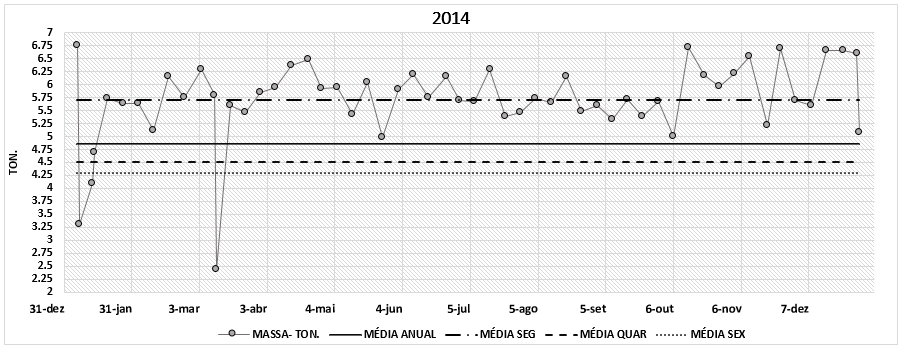
\includegraphics[width=1\textwidth]{produtos/prodtres/image111}
		\end{minipage}
		\begin{minipage}{1.3\textwidth}
			\centering
			\includegraphics[width=1\textwidth]{produtos/prodtres/image112}
			\label{fig:image112}
		\end{minipage}
	\end{figure}
	
		\begin{figure}[h]
		\centering
		\caption*{Segundas-feira}
		\begin{minipage}{1.4\textwidth}
			\centering
			\label{fig:image113}
			\includegraphics[width=1\textwidth]{produtos/prodtres/image113}
		\end{minipage}
		\begin{minipage}{1.4\textwidth}
			\centering
			\includegraphics[width=1\textwidth]{produtos/prodtres/image114}
			\label{fig:image114}
		\end{minipage}
	\end{figure}

\end{landscape}

\FloatBarrier

%\section{Quartas-feira}

\begin{landscape}
	
	\begin{figure}[h]
		\centering
		\caption*{Quartas-feira}
		\begin{minipage}{1.4\textwidth}
			\centering
			\label{fig:image115}
			\includegraphics[width=1\textwidth]{produtos/prodtres/image115}
		\end{minipage}
		\begin{minipage}{1.4\textwidth}
			\centering
			\includegraphics[width=1\textwidth]{produtos/prodtres/image116}
			\label{fig:image116}
		\end{minipage}
	\end{figure}
	
	\begin{figure}[h]
		\centering
		\caption*{Quartas-feira}
		\begin{minipage}{1.4\textwidth}
			\centering
			\label{fig:image118}
			\includegraphics[width=1\textwidth]{produtos/prodtres/image118}
		\end{minipage}
		\begin{minipage}{1.4\textwidth}
			\centering
			\includegraphics[width=1\textwidth]{produtos/prodtres/image117}
			\label{fig:image117}
		\end{minipage}
	\end{figure}
	
\end{landscape}

\FloatBarrier

%\section{Sextas-feira}

\begin{landscape}
	
	\begin{figure}[h]
		\centering
		\caption*{Sextas-feira}
		\begin{minipage}{1.4\textwidth}
			\centering
			\label{fig:image119}
			\includegraphics[width=1\textwidth]{produtos/prodtres/image119}
		\end{minipage}
		\begin{minipage}{1.4\textwidth}
			\centering
			\includegraphics[width=1\textwidth]{produtos/prodtres/image120}
			\label{fig:image120}
		\end{minipage}
	\end{figure}
	
	\begin{figure}[h]
		\centering
		\caption*{Sextas-feira}
		\begin{minipage}{1.4\textwidth}
			\centering
			\label{fig:image121}
			\includegraphics[width=1\textwidth]{produtos/prodtres/image121}
		\end{minipage}
		\begin{minipage}{1.4\textwidth}
			\centering
			\includegraphics[width=1\textwidth]{produtos/prodtres/image122}
			\label{fig:image122}
		\end{minipage}
	\end{figure}
	
\end{landscape}

\FloatBarrier

\chapter{}

Este apêndice apresenta as Listas de Presença referentes as Oficinas Participativas realizadas no município de Monteiro Lobato, no período de agosto a outubro de 2018. A metodologia e resultados para essas Oficinas encontram-se descritas na secção \ref{oficinas} deste produto.

\newpage
\section{Oficina participativa com os professores}

\begin{figure}[h]
	\centering
	\includegraphics[width=.75\linewidth]{produtos/prodtres/image123}
	\caption*{}
	\label{fig:image123}
\end{figure}

\FloatBarrier
\newpage
\section{Oficina participativa com o bairro centro}
\begin{figure}[h]
	\centering
	\includegraphics[width=.75\linewidth]{produtos/prodtres/image124}
	\caption*{}
	\label{fig:image124}
\end{figure}

\FloatBarrier
\newpage
\section{Oficina participativa com o bairro Souzas}
\begin{figure}[h]
	\centering
	\includegraphics[width=.75\linewidth]{produtos/prodtres/image125}
	\caption*{}
	\label{fig:image125}
\end{figure}

\FloatBarrier
\newpage
\section{Oficina participativa com o bairro São Benedito}
\begin{figure}[h]
	\centering
	\includegraphics[width=.75\linewidth]{produtos/prodtres/image126}
	\caption*{}
	\label{fig:image126}
\end{figure}

	\EndNoToc
%
\let\cleardoublepage\clearpage
%\addcontentsline{toc}{section}{Anexos}
\anexos
	\BeginNoToc
%	\titleformat{\subsection}
{\Large\bfseries\scshape\raggedright}
{\thesubsection}{1em}
{}
\titleformat{\subsubsection}
{\Large\bfseries\scshape\raggedright}
{\thesubsubsection}{1em}
{}
\titlespacing*{\section}{0pt}{*4}{*2}
\titlespacing*{\subsection}{0pt}{*4}{*2}
\titlespacing*{\subsubsection}{0pt}{*0}{*0}

\chapter{Definição da estratégia de mobilização e participação social}
\section{Mobilização Social}
De acordo com a PNRS (BRASIL, 2010), o controle social deverá ser realizado de modo que seja possível à sociedade ter acesso à informação e participar da implementação e da avaliação de políticas públicas voltadas ao tema dos resíduos sólidos. Assim, todos os mecanismos, ações e procedimentos que viabilizem esses objetivos de participação pública poderão ser entendidos como estratégias de controle social. 

Para promoção da participação e do controle social, são necessárias estratégias de comunicação e divulgação, e estratégias de mobilização social (ROMANI; SEGALA, 2014). De acordo com o Ministério do Meio Ambiente (MMA) e o ICLEI-Brasil (2012), a mobilização social pode ser entendida como uma mudança não apenas comportamental, mas também de hábitos, a qual ocorre, principalmente, por meio do diálogo e de ações orientadoras e provocativas, por parte do poder público. 

As estratégias para a mobilização social podem ser materializadas de diversas formas, a depender do alcance que se pretende. Para elaboração do Plano Nacional de Resíduos Sólidos, de abrangência nacional, foram adotadas audiências públicas regionais, audiência pública nacional e diversas consultas via internet (ROMANI; SEGALA, 2014). Em outro exemplo, em escala local, o município de São José dos Campos adotou as seguintes estratégias de mobilização social (SÃO JOSÉ DOS CAMPOS, 2015):
\begin{enumerate}
	\item Conscientização em domicílio;
	\item Palestras em ambientes públicos, como escolas, igrejas, ONGs, empresas etc.;
	\item Reuniões com diversos segmentos sociais;
	\item Mutirões de conscientização ambiental;
	\item Programa Lixo-Tour.
\end{enumerate}

\section{Metodologia}

As estratégias de mobilização social para o Plano Municipal de Gestão Integrada de Resíduos Sólidos de Monteiro Lobato foram elaboradas de modo que fosse possível conclamar toda a comunidade lobatense à participação no processo de construção e implementação do PMGIRS. Procurou-se levar em consideração, além das principais práticas já adotadas em outros planos do mesmo tema, as principais estratégias já adotadas no município, em iniciativas anteriores de mobilização social dentro do tema de gestão de resíduos sólidos, bem como a opinião de moradores e autoridades municipais. Essas estratégias foram desenvolvidas em três etapas:
\begin{enumerate}
	\item Diagnóstico, diálogo inicial e percepção de como a comunidade pode participar da elaboração e implementação do PMGIRS;
	\item Identificação de estratégias de mobilização social adotadas anteriormente pelo município;
	\item Estratégias para mobilizar a comunidade durante a elaboração, implementação, fiscalização e revisão do PMGIRS.
\end{enumerate}

\section{Diagnóstico e diálogo inicial}
 De acordo com vereadores e secretários municipais de Monteiro Lobato, a população lobatense pode ser classificada conforme descrito a seguir: 
 
\subsection{Morador tradicional}

Muito religioso (em sua maioria, católicos e evangélicos) esse tipo de morador é conservador, às vezes reacionário, avesso a mudanças radicais, 
Habita as áreas centrais do município, possui maior poder de compra e de decisão, em sua grande parte são donos de empreendimentos e estabelecimentos na cidade, ocupam cargos importantes no município, como os de vereadores e conselheiros da prefeitura. Tem maior escolaridade que os demais moradores, com vivências em outras regiões e municípios maiores, de grandes centros culturais, tais como as capitais estaduais brasileiras e de outros países do mundo.

\subsection{Morador de áreas rurais}

Representa a maioria dos moradores do município com traços mais tímido, menos participativos. O acesso a esse tipo de morador é restrito a pessoas de sua confiança e deve ser feito com grande cuidado. Esse tipo de morador possui baixa ou nenhuma escolaridade e pouca vivência fora dos limites do município.

\subsection{Novo morador}

É imigrante de outro município brasileiro, em geral, maior do que Monteiro Lobato.  O novo morador busca a tranquilidade característica do município, além de desfrutar do ambiente natural e fugir de problemas socioambientais de grandes centros urbanos. Esse tipo de morador possui nível de escolaridade maior do que a média do município, podendo manifestar opiniões sobre assuntos relacionados ao contexto municipal de forma elaborada, argumentada e crítica. O novo morador simpatiza-se com a ideia de conservação do ambiente natural e tranquilo, estando disposto a manifestar-se ativamente para que assim o ambiente do município seja mantido.

\subsection{Morador jovem}

Moradores jovens tendem a acessar a internet e as redes sociais com mais frequência, sendo mais ativos virtual do que fisicamente. É uma parcela da população que pouco se interessa em participar ativamente em atividades para a melhoria da qualidade ambiental do município. O jovem de Monteiro Lobato possui baixo nível de escolaridade, sendo que a maioria não estuda nem trabalha. Esse tipo de morador possui pouco interesse em sair da cidade e dificilmente dialoga sobre questões que extrapolam os assuntos compartilhados em redes sociais das quais participa.

\section{Estratégias adotadas anteriormente pelo município}

Grande parte das estratégias de educação ambiental e mobilização social para o desenvolvimento de ações de cuidado com os resíduos sólidos do município foram desenvolvidas tendo como núcleo de ação as escolas de ensino básico. Muitas dessas ações tinham como referencial principal o atual Instituto Pandavas, com o qual a Prefeitura estabeleceu parcerias de ação social e cuidado com o meio ambiente. O Instituto Pandavas – Núcleo de Educação, Cultura e Ações Socioambientais, existe desde 2008 e se propõe a dar continuidade aos trabalhos de educação ambiental, cidadania, justiça social e conservação da qualidade ambiental do município, desenvolvidos anteriormente pelo Centro Pedagógico Casa dos Pandavas – CPCP (PANDAVAS, 2017).

Nas décadas de 1990 e 2000, havia, no Centro Pedagógico Casa dos Pandavas, uma ONG chamada GARP – Grupo Ambientalista Ribeirão dos Pássaros. Essa ONG desenvolvia atividades para envolver pais, alunos e professores em ações e movimentos voltados à educação ambiental relacionada aos resíduos sólidos. Foram feitos mutirões, em que foram coletados materiais recicláveis nas ruas da cidade, em terrenos baldios e outras áreas de descarte irregular, com auxílio de caminhões que transportavam os resíduos coletados. Os mutirões foram feitos predominantemente em bairros da zona urbana; e em alguns locais da zona rural, como no Sousa e no São Benedito. Além disso, a ONG organizou a entrega de materiais escritos, nas áreas urbanas da cidade, de porta em porta, entre 1998 e 2000, com o objetivo de promover a educação ambiental e uma cultura de cuidado com os resíduos sólidos, visando a separação dos materiais em secos e úmidos. Na época, havia tratamento diferenciado para materiais recicláveis, os quais ficavam armazenados e eram triados em um galpão mantido pela Prefeitura.

Atualmente, não há continuidade de movimentos de educação ambiental envolvendo a comunidade lobatense da maneira como existia na época do CPCP; no entanto, trabalhos de cultura cinematográfica vêm sendo desenvolvidos, envolvendo jovens e adolescentes na discussão de temas importantes para o município. A Prefeitura participa ativamente na elaboração de vídeos e na escolha dos temas a serem abordados. 

\section{Estratégias propostas}

Levando em consideração as principais características do morador lobatense, além dos métodos já adotados no município com êxito para obtenção de participação da sociedade em projetos, foram elaboradas estratégias de participação e mobilização social, por meio das quais será possível convidar, envolver e esclarecer a comunidade sobre assuntos pertinentes à elaboração, implementação, fiscalização e revisão do PMGIRS. Todas as estratégias apresentadas a seguir foram validadas e elaboradas em consonância com a opinião dos secretários de meio ambiente e de educação, prefeita e vereadores, além de assessores técnicos atuantes na Prefeitura. Na \autoref{fig:danielepub} é possível visualizar o registro do dia em que ocorreu a entrevista com vereadores, a secretária de meio ambiente e técnicos assessores do serviço público municipal.

\begin{figure}
	\centering
	\includegraphics[width=\linewidth]{produtos/produm/danielepub}
	\caption{Encontro do estagiário Daniel com vereadores de Monteiro Lobato e integrantes da secretaria de meio ambiente}
	\label{fig:danielepub}
\end{figure}

O conteúdo das mensagens a serem distribuídas aos moradores, com o intuito de mobilização social, poderão abranger aspectos relacionados à logística dos resíduos (para coleta e para a destinação final), localização e tipo de material a ser usado em novas lixeiras, redução de geração de resíduos, custos do sistema de gestão e possibilidade de redução de custos em função da redução da geração dos resíduos, segurança no manuseio de resíduos, valorização do profissional que atua em contato direto com os resíduos, além da importância de separação dos tipos de resíduos gerados, na fonte geradora, entre inúmeros outros possíveis. Uma vez estabelecido o canal de comunicação com cada morador, poderão ser agendadas audiências públicas, reuniões entre líderes comunitários e representantes políticos, palestras, bem como festivais e eventos culturais para congregação de todos os interessados ou qualquer outra forma de comunicação e diálogo que convier no momento em que ocorrer a necessidade de diálogo e disseminação de informação entre comunidade e equipe responsável pela elaboração e implementação do PMGIRS.

No entanto, ressalta-se que o conteúdo específico a ser divulgado em cada etapa (elaboração, implementação, fiscalização e revisão) deverá ser definido em conjunto com todos os envolvidos e responsáveis pela elaboração do PMGIRS, o que inclui técnicos e servidores municipais. Nesta seção, será enfatizada a forma com que cada tipo de morador de Monteiro Lobato deverá ser abordado. Nesse contexto, as mensagens mobilizadoras deverão ser transmitidas com o intuito de provocar, orientar, mas também incitar o diálogo com a comunidade lobatense (MMA; ICLEI-BRASIL, 2012).

\subsection{Morador tradicional}

Deverá ser mobilizado de duas maneiras:
\begin{itemize}
	\item contato direto e pessoal, de porta em porta;
	\item contato indireto, por meio de igrejas e parcerias com líderes religiosos do município.
\end{itemize}

Na \autoref{fig:estrategmobi}, são apresentadas as etapas a serem seguidas para que se alcance o máximo de participantes de hábitos tradicionais.

\begin{figure}[h!]
	\centering
	\includegraphics[width=\linewidth]{produtos/produm/estrategmobi}
	\caption{Estratégia de mobilização de moradores tradicionais}
	\label{fig:estrategmobi}
\end{figure}

Poderão ser reunidos como voluntários quaisquer alunos, servidores públicos ou munícipes devidamente treinados para conversar com o morador tradicional. No treinamento, deverão ser definidos:

\begin{itemize}
	\item Vestes a serem usadas;
	\item Linguagem e forma de abordagem;
	\item Conteúdo a ser transmitido;
	\item Tempo de fala;
	\item Conhecimento mínimo sobre o PMGIRS para que o visitante possa responder a eventuais
	perguntas dos moradores.
\end{itemize}

Em entrevista realizada na época de elaboração do plano, na câmara de vereadores de Monteiro Lobato, foi acordado entre vereadores e a secretária de meio ambiente, que os mesmos poderiam contribuir no acesso a líderes religiosos do município.

Deve-se também ressaltar a importância do estimulo fornecido pelo poder publico para que as associações de bairro realizem ações de mobilização mais efetiva da população.

\subsection{Morador de áreas rurais}

A mobilização da comunidade de áreas rurais será mais efetiva, caso as informações sobre a elaboração e implementação do PMGIRS sejam transmitidas por meio de pessoas de sua confiança, tendo como núcleo de ação as escolas rurais de ensino básico. Para que isso aconteça, apresenta-se na \autoref{fig:estrategmobiarearural} a estratégia por meio da qual será alcançada a participação comunitária, em etapas de execução na forma de um fluxograma.

\begin{figure}[h!]
	\centering
	\includegraphics[width=\linewidth]{produtos/produm/estrategmobiarearural}
	\caption{Estratégia de mobilização de moradores de áreas rurais}
	\label{fig:estrategmobiarearural}
\end{figure}

A pessoa encarregada de conversar com os coordenadores de escolas rurais deverá saber se portar, comunicar, e transmitir de forma clara e precisa a necessidade de envolvimento das escolas na elaboração e implementação do PMGIRS. A tarefa poderá ser executada por um aluno estagiário ou não, com ou sem a apresentação de slides. Uma vez alcançado o comprometimento dos coordenadores de escolas e incorporada a temática de planejamento municipal da gestão dos resíduos sólidos no plano pedagógico de ensino, os alunos poderão ser envolvidos por meio de atividades diversas, tais como:
\begin{enumerate}
	\item Gincanas; 
	\item Redações; 
	\item Apresentações sobre o tema durante as aulas; 
	\item Estimulo de redução de consumo; 
	\item Visitas a locais de tratamento de resíduos, tais como um aterro sanitário ou uma cooperativa; 
	\item Mutirões para coleta de resíduos descartados irregularmente na área rural. 
\end{enumerate}

Com o apoio de coordenadores, educadores e alunos, os adultos, pais e familiares de áreas rurais, poderão ser envolvidos com maior facilidade, em encontros, reuniões, eventos escolares, etc. Assim, espera-se que um maior número da comunidade rural participará ou estará ciente de que sua participação é importante para o sucesso do PMGIRS.

\subsection{Turistas e visitantes}
A principal preocupação manifestada por autoridades municipais, em relação à visitação e turismo, refere-se ao respeito à dinâmica de separação dos tipos de resíduos e conservação da limpeza em todas as regiões visitadas, tanto no centro da cidade, como em pousadas mais afastadas do centro.  Além disso, foi ressaltada a importância de colaboração, por parte de todos os transeuntes (visitantes ou não), com as práticas e hábitos a serem implementados no município, em função das ações de implementação do PMGIRS. Assim, tendo como base essas preocupações principais, foi elaborada a estratégia para mobilização de visitantes e turistas, apresentada na \autoref{fig:estrategmobiturista}.

\begin{figure}[h!]
	\centering
	\includegraphics[width=\linewidth]{produtos/produm/estrategmobiturista}
	\caption{Estratégia de mobilização de visitantes e turistas}
	\label{fig:estrategmobiturista}
\end{figure}

Turistas e visitantes não são moradores; mas frequentam restaurantes, pousadas, hotéis e eventos culturais, gerando resíduos e podendo degradar a qualidade ambiental do município. Assim, deverão ser contatados a partir dos locais que frequentam, a partir de diálogo com donos de pousadas, hotéis, restaurantes e, eventualmente, coordenadores de festivais e eventos culturais em que haja aglomeração de pessoas, tais como o carnaval e festas de culinária e personagens de literatura infantil. A partir do diálogo com os gestores de estabelecimentos e locais turísticos, as ações de mobilização com foco nas necessidades de implementação ou elaboração do PMNGIRS deverão ser elaboradas e executadas.


\subsection{Morador jovem}

Como jovem, entende-se o conjunto de moradores com idades entre 15 e 24 anos (IBGE, 2017).  Esse público, deverá ser contatado por meio de estratégias de encontros virtuais, conforme apresentado na \autoref{fig:estrategmobijovem}.

\begin{figure}[h!]
	\centering
	\includegraphics[width=\linewidth]{produtos/produm/estrategmobijovem}
	\caption{Estratégia de mobilização de moradores jovens}
	\label{fig:estrategmobijovem}
\end{figure}

O responsável por cuidar e realizar publicações na página criada do Facebook deverá ser definido em conjunto com autoridades do município e membros da equipe acadêmica responsável pela elaboração do PMGIRS. Sugere-se que a frequência de publicações seja diretamente proporcional à frequência com que novas ações sejam realizadas.

Para saber se o número de indivíduos com acesso à página é representativo ou não, sugere-se a adoção de uma proporção de representatividade a ser definida em conjunto com autoridades municipais. Essa proporção poderá ser, por exemplo, igual ou superior a 70\% da população de jovens do município (IBGE, 2017). Maiores informações sobre amostras significativas estão disponíveis em Bussab e Bolfarine (2005).


\section{Oficina para a apresentação do diagnóstico e discussões acerca da realização do prognóstico}

\subsection{Metodologia}

A oficina participativa é um instrumento amplamente utilizado para aproximar entidades públicas ou privadas de comunidades que são diretamente afetadas por ações, empreendimento ou políticas que possam alterar o cotidiano de uma população. Nessa prática, procura-se informar as condições dos locais que receberão tais ações, os estudos efetuados e resultados obtidos até o momento. A informação é passada de forma simples, direta e transparente cientificando e elucidando as informações à população, quanto ao andamento e às possíveis alterações que ocorrerão dentro de escopo apresentado.

A participação da população nessa etapa é de suma importância para o andamento das ações pretendidas, pois será neste momento que a população terá a possibilidade de fazer críticas/considerações sobre os dados apresentados e sobre as ações propostas, podendo também propor alternativas mais condizentes com as necessidades locais, bem como se informar sobre o andamento das ações.

Em Monteiro Lobato foram efetuadas 4 oficinas participativas (tabela q), de um total de 5 oficinas previstas, nas quais foi explicado aos participantes as condições relacionadas à produção, descarte, transporte e destinação dos resíduos sólidos do município. A estrutura da oficina é baseada em uma metodologia conhecida "Word Café". Esse sistema é um processo participativo com capacidade de trabalhar a diversidade e complexidade no grupo, fazendo emergir a inteligência coletiva. O processo é organizado de forma que as pessoas circulem entre os diversos grupos e conversas, conectando e semeando as ideias, tornando visível a inteligência e a sabedoria do coletivo. A oficina foi dividida em 3 etapas com 20 minutos cada: 

\begin{itemize}
	\item Apresentação dos dados municipais referentes aos resíduos gerados majoritariamente pela população (Resíduo Sólidos Urbano (RSU), Resíduos de Construção Civil (RCC), Resíduos de Serviços de Saúde (RSS) e logística reversa);
	\item Dinâmica inicial em grupo, por classe de resíduo ou conjunto de classes;
	\begin{itemize}
	\item Discussão interna feita pelos participantes sobre problemas relacionados à(s) classe(s) e seus possíveis motivos;
	\item descrição escrita em papéis separados sobre problemas e motivos destes problemas percebidos pela população;
	\item apresentação para todos os participantes das considerações feitas em grupo, seguida de rodas de discussão dos conteúdos apresentados e aprimoramento das ideias.
	\end{itemize}
	\item Dinâmica final em grupo, por classe de resíduo ou conjunto de classe;
	\begin{itemize}
	\item discussão interna sobre possíveis soluções relacionados à(s) classe(s) e como proporcionar seu acontecimento;
	\item descrição escrita em papéis separados sobre possíveis soluções e métodos para sua execução;
	\item apresentação para todos participante das considerações feitas seguida de rodas de discussão dos conteúdos apresentados e aprimoramento das ideias.
	\end{itemize}
\end{itemize}

A formação de grupos será realizada de acordo com os grandes grupos de classificação de resíduo, sendo que deve haver no mínimo dois grupos ou no máximo quatro, a escolha deve ser realizada de acordo com o número de participantes da oficina. Os objetivos principais são: promover a interação em conjunto dos participantes para identificar os principais problemas do município relacionados ao tratamento dos resíduos sólidos no município de Monteiro Lobato. Além disso deve ocorrer uma discussão mais especifica sobre os problemas comuns relacionados aos resíduos a que foram atribuídos ao grupo, bem como as soluções viáveis para mitigar os problemas encontrados e a magnitude dos impactos negativos e positivos, dos problemas e das soluções respectivamente. A etapa final da oficina consiste na troca de informações entre os grupos com apresentação das ideias e uma discussão entre os participantes.

\thispagestyle{headfootimage}
	\EndNoToc
	\newcommand\capafimimageheight{\paperheight}

\newsavebox{\capafimimage}
\sbox\capafimimage{%
	\tikz{
		\clip(0,0)rectangle(\paperwidth,-\paperheight);
		\node[inner sep=0pt,outer sep=0pt,anchor=north west]{%
			\includegraphics[width=\paperwidth, height=\paperheight]{src/layout/capafim}};
	}%
}

\DeclareNewLayer[
background,
area={0pt}{0pt}{\paperwidth}{\paperheight},
contents={\usebox\capafimimage}
]{capafimimage}

\DeclarePageStyleByLayers{capafimlayimage}{%
	capafimimage
}
\thispagestyle{capafimlayimage}
{\phantom{capafim}}\thispagestyle{capafimlayimage}

\pagebreak

\end{document}